%%%%%%%%%%%%%%%%%%%%%%%%%%%%%%%%%%%%%%%%%%%%%%%%%%%%%%%%%%
%% 
%% Solutions of Exercises MARK: -
%% 
%%%%%%%%%%%%%%%%%%%%%%%%%%%%%%%%%%%%%%%%%%%%%%%%%%%%%%%%%%

\chapter*{Solutions of Exercises}

%%%%%%%%%%%%%%%%%%%%%%%%%%%%%%%%%%%%%%%%%%%%%%%%%%%%%%%%%%
%% 
%% Axioms of diffeology
%% 
%%%%%%%%%%%%%%%%%%%%%%%%%%%%%%%%%%%%%%%%%%%%%%%%%%%%%%%%%%
\SkipTocEntry\section*{Axioms of Diffeology}

\solexref{Equivalent-axiom-of-covering}
(Equivalent axiom of covering) 
Consider the three axioms D1, D2, D3
\art{Diffeologies-and-diffeological-spaces}.
From the axiom D1 the constants maps
cover ${\X}$, thus D1' is satisfied. Hence, D1, D2, D3 imply D1', D2,
D3. Conversely, consider D1', D2, and D3. Let $x$ be a point
of $\X$. By D1' there exists a plot
$\P : \U \to \X$ such that $x$ belongs to $\P(\U)$. Let $r$ in $\U$
such that ${\P}(r) = x$. Now let $n$ be any integer. Let $\bmr: \RR^n
  \to {\U}$ be the constant parametrization mapping every point of $\RR^n$
to $r$. The composition ${\P} \circ \bmr$ is the constant 
parametrization $\bmx$ mapping $\RR^n$ to
$x$. Since $\bmr$ is smooth and thanks to D3 the parametrization 
${\P} \circ \bmr$ is a plot of $\X$. Hence, D1 is satisfied and D1',
D2, D3 imply D1, D2, D3. Therefore, the axioms D1, D2, D3 are
equivalent to the axioms D1', D2, D3.
\endsolexref

\solexref{Equivalent-axiom-of-locality} (Equivalent axiom of locality) 
Consider the three axioms D1, D2, D3
\art{Diffeologies-and-diffeological-spaces}. Let ${\P}: {\U} \to {\X}$
be a parametrization. Assume that for any point $r$ of
${\U}$ there exists an open neighborhood ${\V}_r$ of $r$ such that
${\P}_r = {\P}\restriction {\V}_r$ belongs to $\cD$. The
family $({\P}_r)_{r \in {\U}}$ is a compatible family
of elements of $\cD$ with ${\P}$ as supremum. Thanks to
the axiom D2, $\P$ belongs to $\cD$, and D2' is
satisfied. Hence, D1, D2, D3 imply D1, D2', D3.
Conversely, consider D1, D2' and D3. Now, let 
$\{ \P_i : \U_i \to \X \}_{i \in \cI}$ be a family of
compatible $n$-parametrizations, and let $\P:
  \U \to \X$ be the supremum of the family. Let
$r$ be any point of $\U$. By definition of $\P$,
there exists $\P_i: \U_i \to \X$
with $r \in \U_i$ such that $\P \restriction \U_i =
  \P_i$. Thus, the axiom D2' is satisfied. Hence, D1, D2',
D3 imply D1, D2, D3. Therefore, the axioms D1, D2,
D3 are equivalent to the axioms D1, D2', D3. 
\endsolexref

\solexref{Global-plots-and-diffeology} (Global plots and diffeology) 
Let $\P : \U \to \X$ be an $n$-parametrization belonging to $\cD$. 
For all points $r$ in $\U$ there exists a real $\epsilon > 0$ such that 
the open ball $\B(r,\epsilon)$,
centered at $r$, of radius $\epsilon$, is contained in $\U$. Since the
inclusion $\B(r,\epsilon) \subset \U$ is a smooth parametrization, the
restriction $\P \restriction \B(r,\epsilon)$ belongs to $\cD$. Now,
the following parametrization 
$$
\varphi : \B(r,\epsilon) \to \B(0,1),
  \qmbox{defined by} \varphi : s \mapsto s' = {1 \over \epsilon} (s - r),
  $$
is a diffeomorphism.
Next, let $\psi : \B(0,1) \to \RR^n$, and then $\psi^{-1} : \RR^n \to \B(0,1)$,
given by
$$
\psi(s) = { s \over \sqrt{1 - \norm{s}^2}} \qmbox{and}
  \psi^{-1}(s') = { s' \over \sqrt{1 + \norm{s'}^2}}.
  $$ 
The parametrization $\psi$ is a diffeomorphism. 
Hence, $\phi = \psi \circ \varphi$ is a diffeomorphism
from $\B(r,\epsilon)$ to $\RR^n$. Then, thanks to the axiom of smooth
compatibility, the global parametrization $(\P \restriction
  \B(r,\epsilon)) \circ \phi^{-1} : \RR^n \to \X$ belongs to
$\cD$. By hypothesis, it also belongs to $\cD'$.
Thus, thanks again to the axiom of smooth
compatibility, the parametrization $[(\P \restriction \B(r,\epsilon))
\circ \phi^{-1}] \circ \phi = \P \restriction \B(r,\epsilon)$ 
belongs to $\cD'$. Now, $\P$ being the supremum of a compatible family of
elements of $\cD'$, thanks to the
axiom of locality of diffeology, $\P$ is an element of $\cD'$.
Therefore, $\cD \subset \cD'$, exchanging $\cD$ and $\cD'$ gives
$\cD' \subset \cD$, and finally $\cD = \cD'$.
\endsolexref

%%%%%%%%%%%%%%%%%%%%%%%%%%%%%%%%%%%%%%%%%%%%%%%%%%%%%%%%%%
%% 
%% Smooth maps and category Diffeology
%% 
%%%%%%%%%%%%%%%%%%%%%%%%%%%%%%%%%%%%%%%%%%%%%%%%%%%%%%%%%%
\SkipTocEntry\SkipTocEntry\section*{Smooth Maps and Category Diffeology}

\solexref{Diffeomorphisms-between-irrational-tori}
(Diffeomorphisms between irrational tori) 
Let $\P : \U \to \T_\alpha$ be a parametrization. Let us say that {\em
$\P$ lifts locally along $\pi_\alpha$, at the point $r \in \U$\/}, if there
exist an open neighborhood $\V$ of $r$ and a smooth parametrization 
$\Q : \V \to \RR$ such that $\pi_\alpha \circ \Q = \P \restriction \V$. 
Now, the property (\blacksnow) writes: $\P$ is a plot if it lifts locally along
$\pi_\alpha$, at every point of $\U$.

\alinea{1)} Let us check, following \art{A-diffeology-for-the-circle},
that the property (\blacksnow) defines a diffeology. 

\alinea{D1} --- Since $\pi_\alpha$ is surjective, for every point $\tau \in \T_\alpha$ 
there exists $x \in \RR$ such that $\tau = \pi_\alpha(r)$.
Then, $\bmx : r \mapsto x$ is a lift in $\RR$ 
of the constant parametrization $\btau : r \mapsto \tau$.

\alinea{D2} --- The axiom of locality is satisfied by the very definition of $\cD$.

\alinea{D3} --- Let $\P : \U \to \T_\alpha$ satisfying (\blacksnow). Let $\F : \U'
  \to \U$ be a smooth para\-met\-ri\-za\-tion. Let $r'$ be a point of $\U'$, let
$r = \F(r')$, let $\V$ be an open neighborhood of $r$ and $\Q$ be a smooth
parametrization in $\RR$ such that $\pi_\alpha \circ \Q = \P
  \restriction \V$. Let $\V' = \F^{-1}(\V)$ and $\Q' = \Q \circ \F$,
defined on $\V'$. Then, 
$\pi_\alpha \circ \Q' = (\P \circ \F) \restriction \V'$.  

\alinea{2)} Let us consider $f \in \Cinfty(\T_\alpha,\RR)$. Since $\pi_\alpha$
and $f$ are smooth, the map $\F = f \circ \pi_\alpha$
belongs to $\Cinfty(\RR,\RR)$
\art{composition-of-smooth-maps}. But since
$\pi_\alpha(x + n + \alpha m) = \pi_\alpha(x)$, for every
$n,m$ in $\ZZ$, we also have $\F(x + n + \alpha m) = \F(x)$. 
Hence, $\F$ is smooth and constant on a dense
subset of numbers $\ZZ + \alpha \ZZ \subset \RR$ (for $x = 0$). Thus,
$\F$ is constant and therefore $f$ is constant. In other
words, $\Cinfty(\T_\alpha,\RR) = \RR$.

\alinea{3)} Let us consider a smooth map 
$f : \T_\alpha \to \T_\beta$. 
Note that, since $\pi_\alpha$ satisfies
obviously (\blacksnow), $\pi_\alpha$ is a plot of
$\T_\alpha$. Then, by definition of differentiability
\art{Smooth-maps}, $f \circ \pi_\alpha$ is a
plot of $\T_\beta$. Hence, for every real $x_0$ there
exist an open neighborhood $\V$ of $x_0$ and a smooth
parametrization $\F : \V \to \RR$ such that 
$\pi_\beta \circ \F = (f \circ \pi_\alpha) \restriction \V$. 
Since $\V$ is an open subset of $\RR$ containing $x_0$, we can
choose $\V$ as an interval centered at $x_0$. For all
real numbers $x$ and all pairs $(n,m)$ of integers such
that $x + n + \alpha m$ belongs to $\V$, the identity
$\pi_\beta \circ \F = (f \circ \pi_\alpha) \restriction \V$ 
writes  
$\pi_\beta \circ \F(x + n + \alpha m)  = f \circ \pi_\alpha(x + n + \alpha m) 
= f \circ \pi_\alpha(x) = \pi_\beta \circ \F(x)$. 
Thus, there exist two integers $n'$ and $m'$ such that
\begin{equation}
  \renewcommand{\theequation}{$\spadesuit$}
  \F(x + n + \alpha m) = \F(x) + n' + \beta m'.
\end{equation} 
Since $\beta$ is irrational, for every such $x$, $n$ and $m$, 
the pair $(n',m')$ is unique.
%
There exists an interval $\cJ \subset \V$ centered at $x_0$ and an
interval $\cO$ centered at $0$ such that for every $x \in \cJ$ and for
every $n + \alpha m \in \cO$, $x + n + \alpha m \in \V$. Since $\F$ is
continuous and since $\ZZ + \alpha \ZZ$ is totally discontinuous, $n' +
  \beta m' = \F(x + n + \alpha m) - \F(x)$ is constant as function of
$x$. But $\F$ is smooth, the derivative of the identity ($\spadesuit$),
with respect to $x$, at the point $x_0$, gives $\F'(x_0 + n + \alpha m)
  = \F'(x_0)$. Then, since $\alpha$ is irrational, $\ZZ + \alpha \ZZ \cap
    \cO$ is dense in $\cO$ and since $\F'$ is continuous, $\F'(x) =
      \F'(x_0)$,  for all $x \in \cJ$. Hence, $\F$ restricted to $\cJ$ is
affine, there exist two numbers $\lambda$ and $\mu$ such that 
\begin{equation}
  \renewcommand{\theequation}{$\clubsuit$}
  \F(x) = \lambda x + \mu \qmbox{for all} x \in \cJ.
\end{equation} 
Note that, by density of $\ZZ +
  \alpha \ZZ$, $\pi_\alpha(\cJ) = \T_\alpha$. Hence $\F$
defines completely the function $f$.
Now, applying $(\spadesuit)$ to the expression $(\clubsuit)$ of $\F$, we
get for all $n + \alpha m \in \cO$
\begin{equation}
  \renewcommand{\theequation}{$\diamondsuit$}
  \lambda \times (n + \alpha
  m ) \in \ZZ + \beta \ZZ. 
\end{equation}
Let us show that actually $(\diamondsuit)$ is satisfied for all 
$n + \alpha m$ in $\ZZ + \alpha \ZZ$. Let $\cO = ]-a,a[$, and let us take
$a$ not in $\ZZ + \alpha \ZZ$, even if we have to shorten 
$\cO$ a little bit. Let $x \in \ZZ + \alpha \ZZ$, and $x >a$. There exists 
$\N \in \NN$ such that $0 < (\N-1)a < x < \N a$, and then $0< x/\N < a$.
Now, by density of $\ZZ + \alpha \ZZ$ in $\RR$, for all $\eta >0$
there exists $y \in \ZZ + \alpha \ZZ$ such that $0 < x/\N - y < \eta$.
Choosing $\eta < a/\N$ we have $0 < x - \N y < \N \eta < a$, and 
$0 < y < x/\N < a$. Thus, since $x - \N y \in \ZZ + \alpha \ZZ \cap \cO$,
$\lambda \times (x- \N y) = \lambda x - \N \times (\lambda y) \in \ZZ + \beta \ZZ$. 
But $y \in  \ZZ + \alpha \ZZ \cap \cO$, thus 
$\lambda y \in \ZZ + \beta \ZZ$, and then $\N \times (\lambda y) \in \ZZ + \beta \ZZ$,
therefore $\lambda x \in \ZZ + \beta \ZZ$.
Now, applying successively $(\diamondsuit)$ to $\alpha$ and $1$, we get
$\lambda \alpha \in \ZZ + \beta \ZZ$ and $\lambda \in \ZZ + \beta \ZZ$.
Let $\lambda \alpha = a + \beta b$ and $\lambda = c + \beta d$. If
$\lambda \neq 0$, then $\alpha = (a + \beta b) / (c + \beta d)$.

\alinea{4)} Let us remark first that, since
$\pi_\alpha(\cJ) = \T_\alpha$, the map $\F$, extended to the whole
$\RR$, still satisfies $\pi_\beta \circ \F = f \circ \pi_\alpha$. Now,
let us assume that $f$ is bijective. Note that $f$ surjective is
equivalent to $\lambda \neq 0$. Let us express that $f$ is
injective: let $\tau = \pi_\alpha(x)$ and  $\tau' = \pi_\alpha(x')$,
if  $f(\tau) = f(\tau')$, then $\tau = \tau'$, that is, $x' = x + n +
  \alpha m$, for some relative integers $n$ and $m$. Using the lifting
$\F$, this is equivalent to: if there exist two integers
$n'$ and $m'$ such that $\F(x') = \F(x) + n' + \beta m'$, then there
exist two integers $n$ and $m$ such that  
$x' = x + n + \alpha m$. But $\F(x) = \lambda x + \mu$, with 
$\lambda \times (\ZZ + \alpha \ZZ) \subset \ZZ + \beta \ZZ$. 
Hence, the injectivity writes: if
$\lambda x' + \mu = \lambda x + \mu + n' + \beta m'$, then 
$x' = x + n + \alpha m$, which is equivalent to: if 
$\lambda y \in \ZZ + \beta \ZZ$,
then $y \in \ZZ + \alpha \ZZ$, and finally equivalent to 
$(1/\lambda) \times (\ZZ + \beta \ZZ) \subset \ZZ + \alpha \ZZ$. 
Now, let us consider the multiplication by $\lambda$, as
a $\ZZ$-linear map, from the $\ZZ$-module $\ZZ + \alpha
  \ZZ$ to  the $\ZZ$-module $\ZZ + \beta \ZZ$, defined in
the respective bases $(1,\alpha)$ and $(1, \beta)$, by
$$
\lambda \times 1 = c + d \times \beta \qmbox{and}
  \lambda \times \alpha = a + b \times \beta.
$$ 
The two modules being identified, by their bases, to 
$\ZZ \times \ZZ$, the multiplication by $\lambda$ and the
multiplication by $1/\lambda$ are represented by the
matrices 
$$ 
\lambda \simeq \L = \begin{pmatrix}c & a \\ d & b\end{pmatrix} 
\qmbox{and} {1 \over \lambda} \simeq  \L^{-1}.
$$ 
Thus, the matrix $\L$ is invertible as a matrix with
coefficients in $\ZZ$, that is, $\L = \GL(2,\ZZ)$, or $ad - bc = \pm 1$.    
\endsolexref

\solexref{Smooth-maps-on-R/Q} (Smooth maps on $\RR/\QQ$)  
This exercise is similar to the
\exref{Diffeomorphisms-between-irrational-tori}, with solution above.

\alinea{1)} Let us consider a smooth map $f : \E_\QQ \to \E_\QQ$.
Since $\pi : \RR \to \E_\QQ$ is a plot, by
definition of differentiability \art{Smooth-maps}, $f \circ \pi$ 
also is a plot of $\E_\QQ$. Hence, for every real
$x_0$ there exist an open neighborhood $\V$ of $x_0$ and a smooth
parametrization $f : \V \to \RR$ such that 
$\pi \circ \F = (f \circ \pi) \restriction \V$. 
Since $\V$ is an open subset of $\RR$ containing $x_0$, 
we can choose  $\V$ to be an interval centered at $x_0$. 
For every real number $x$ and every rational number $q$ 
such that $x + q$ belongs to $\V$, 
the identity $\pi \circ \F = (f \circ \pi) \restriction \V$
writes  
$\pi \circ \F(x + q)  = f \circ \pi(x + q) = f \circ \pi(x) = \pi \circ \F(x)$. 
Thus, there exists a rational number $q'$ such that $\F(x + q) = \F(x) + q'$.
The rational number $q' = \F(x + q) - \F(x)$ is smooth in $x$
and $q$, thus constant in $x$ (see also
\exref{Diffeology-of-Q-in-R}). Hence, taking the
derivative of this identity, at the
point $x_0$, with respect to $x$, we get $\F(x_0 + q) = \F'(x_0)$. Let us
denote $\lambda = \F'(x_0)$. Now, according to the
continuity of $\F$ and the density of $\QQ$ in $\RR$, we have 
$\F(x) = \lambda x + \mu$, where $\mu \in \RR$. 
{\em A priori\/} $\F$ is defined on a smaller neighborhood $\W \subset \V$ of
$x_0$, but by density of $\QQ$ in $\RR$ we
get, as in \exref{Diffeomorphisms-between-irrational-tori},
$\pi(\W) = \E_\QQ$. Thus, $\F$ can be extended to the
whole $\RR$ by the affine map 
$x \mapsto \lambda x + \mu$. 
Now, coming back to the condition $\F(x + q) = \F(x) + q'$, 
we get $\lambda (x + q) + \mu = \lambda x + \mu + q'$, 
that is, $\lambda q = q'$. Thus, $\lambda$ is
some number mapping any rational number into another, hence it
is a rational number. Let us denote it by $q$. Therefore, the map
$f$ being defined by $\pi \circ \F = f \circ \pi$, we
get $f(\tau) = q \tau + \tau'$, where $\tau' = \pi(\mu)$. 
Hence, any smooth map from $\E_\QQ$ to $\EE_\QQ$ is affine. 
Note that $f$ is a diffeomorphism if and only if $q \neq 0$.

\alinea{2)} With similar arguments as in the first question, we can check that
any smooth map $f : \T_\alpha \to \E_\QQ$ is the
projection of an affine map 
$\F : x \mapsto \lambda x + \mu$. But $\F$ needs to satisfy the condition 
$\F(x + n + \alpha m) = \F(x) + q$, where $n$ and $m$ are
integers and $q$ is a rational number. In particular, for 
$n = 1$ and  $m = 0$, this gives  $\lambda \in \QQ$, and for
$n=0$ and $m = 1$, $\lambda \alpha \in \QQ$. But since
$\alpha \in \RR - \QQ$, this is satisfied only for
$\lambda = 0$. And finally $\F$ is constant.

\alinea{3)} The identity $\Cinfty(\E_\QQ,\RR) = \RR$ is analogous to
$\Cinfty(\T_\alpha,\RR) = \RR$ of the second question of
\exref{Diffeomorphisms-between-irrational-tori}. The second part of the
question is similar to  the second question of this exercise, inverting
$\QQ$ and $\ZZ + \alpha \ZZ$. The map $\F$ is affine, $\F : x \mapsto
  \lambda x + \mu$, and for every $q \in \QQ$, there exist two numbers
$n,m \in \ZZ$ such that $\F(x + q) = \F(x) + n + \alpha m$. So, we get
$\lambda q = n + \alpha m$. In particular, for $q = 1$, we get that
$\lambda = a + \alpha b$, where $a,b \in \ZZ$. Hence, for any rational number
$q$, $(a + \alpha b) q = n + \alpha m$, that is, $aq + bq \alpha = n +
  \alpha m$, or $(aq - n) + (bq - m) \alpha = 0$. Since $\alpha \in \RR -
    \QQ$, we get, for all $q \in \QQ$, $aq \in \ZZ$ and $bq \in \ZZ$. But
this implies that $a$ and $b$ are divisible by any integer, thus $a =
0$ and $b = 0$, and therefore $\lambda = 0$. 
\endsolexref

\solexref{Smooth-maps-on-spaces-of-maps}
(Smooth maps on spaces of maps)  We shal denote here the
derivation map $d/dx^k$ by $\phi_k$.

\alinea{1)} The map $\phi_k : \Cinfty(\RR) \to \Cinfty(\RR)$ is
smooth if and only if, for every plot 
$\P : \U \to \Cinfty(\RR)$, the parametrization $\phi_k \circ \P$ is a
plot of $\Cinfty(\RR)$. According to the definition of
the functional diffeology of $\Cinfty(\RR)$
\art{A-diffeology-for-the-sets-of-smooth-maps}, the parametrization
$\phi_k \circ \P$ is a plot of $\Cinfty(\RR)$ if and only if the
parametrization $(r,x) \mapsto (\phi_k \circ \P (r))(x)$ is a smooth
parametrization of $\RR$, that is, if the parametrization 
$$
  \psi_k : (r,x) \mapsto \bigg[{d^k \over dx^k}(\P(r))\bigg](x)
  $$
is smooth. But $\psi_k$ is the $k$-partial derivative, with respect
to $x$, of the parametrization $\PP : (r,x) \mapsto \P(r)(x)$,
$$
  \psi_k(r,x) = {\partial^k \PP \over \partial x^k}(r,x).
  $$
Since, by the very definition of the plots of $\Cinfty(\RR)$
\art{A-diffeology-for-the-sets-of-smooth-maps}, the parametrization
$\PP$ is smooth, all
of its partial derivatives are smooth. They are smooth with respect to
the pair of variables $(r,x)$, by the very definition of the class
$\Cinfty$. Therefore, $\psi_k$ is smooth and $d^k/dx^k$ is a
smooth map from $\Cinfty(\RR)$ to itself.

\alinea{2)} The map $\hat x$ is smooth if and only if, for every
plot $\P : \U \to \Cinfty(\RR)$, the parametrization
$\hat x \circ \P : r \mapsto \P(r)(x)$ is smooth. But,
by the very definition of the functional diffeology
\art{A-diffeology-for-the-sets-of-smooth-maps}, the
parametrization $\PP : (r,x) \mapsto \P(r)(x)$ is
smooth. Since the map $\hat x \circ \P$ is the
composition $\PP \circ j_x$, where $j_x$ is the (smooth)
inclusion $j_x : r \mapsto (r,x)$ from $\U$ to $\U
  \times \RR$, the parametrization $\hat x \circ \P$ is
smooth and $\hat x$ belongs to $\Cinfty(\Cinfty(\RR), \RR)$. 
%
Now, note that for every integer $k$, the map $f \mapsto f^{(k)}(x)$ is
just 
$$
f \mapsto f^{(k)} \mapsto \hat x(f^{(k)}) = \bigg[\hat x \circ
  {d^k \over dx^k}\bigg](f),
$$ 
that is, the composition of two smooth maps, therefore it is smooth
\art{composition-of-smooth-maps}. 

\noindent Hence, each component
of the map 
$$ 
\D_x^k : f \mapsto \bigg(\hat x(f), \bigg(
  \hat x \circ {d \over dx} \bigg)(f), \ldots, \bigg( \hat
  x \circ {d^k \over dx^k} \bigg)(f)\bigg) 
$$ 
is smooth, from $\Cinfty(\RR)$ to $\RR$, and
$\D_x^k : \Cinfty(\RR) \to \RR^{k+1}$ is smooth.

\alinea{3)} From differential calculus in $\RR^n$ we know that, for all
$f \in \Cinfty(\RR)$, the map 
$$ 
\F :  x \mapsto \int_0^x f(t) dt 
$$
is continuous and smooth, with $f$ as derivative. 
Since $\F$ is continuous and $\F' = f$ is smooth, the
primitive $\F$ is smooth. Now, $\I_{a,b}(f) = \F(b) - \F(a)$. 
To prove that $\I_{a,b}$ is smooth we have just
to check that the map $\I : f \mapsto \F$ is smooth. Let
$\P : \U \to \Cinfty(\R)$ be a plot, we have 
$$
\I \circ \P(r) = x \mapsto \int_0^x \P(r)(t) dt = 
\int_0^x \PP(r,t) dt \qmbox{with} \PP(r,x) = \P(r)(x).
$$ 
Now, $\I \circ \P$ is a plot of $\Cinfty(\RR)$ if and only if the
parametrization $(r,x) \mapsto (\I \circ \P(r))(x)$ is
smooth, that is, if and only if the parametrization 
$$
  \cP : (r,x) \mapsto \int_0^x\PP(r,t)\, dt
$$ 
is smooth.
But, by the very definition of the functional diffeology
of $\Cinfty(\RR)$, the parametrization $\PP$ is smooth.
Thus, since the partial derivatives of $\PP$ with respect to
the variables $r$ commute with the integration,
on the one hand we have
$$ 
{\partial^n \over \partial r^n}\cP(r,x) =
  \int_0^x {\partial^n \over \partial r^n}\PP(r,t)\, dt.
$$ 
On the other hand, since the partial derivatives of $\PP$,
with respect to $r$ or $x$, commute, we have, for 
$m \geq 1$ 
$$ 
{\partial^n \partial^m \over \partial r^n
    \partial x^m}\cP(r,x) = {\partial^n \over \partial
    r^n}\bigg[{\partial^m \over \partial x^m} \int_0^x
    \PP(r,t)\, dt \bigg] = {\partial^n \over \partial r^n}
    {\partial^{m-1} \over \partial x^{m-1}} \PP(r,x). 
$$
Therefore, the parametrization $\cP$ is smooth and 
$\I, \I_{a,b} \in \Cinfty(\Cinfty(\RR))$.

\alinea{4)} Checking that the condition 
\xart{A-diffeology-for-the-sets-of-smooth-maps}{($\diamondsuit$)} defines a diffeology is
straightforward. The same arguments as for
\art{A-diffeology-for-the-circle} can be used, or the
general construction of subset diffeology, described in
\art{Subspaces-and-subset-diffeology}. Now, the derivative is
smooth and, restricted to
$\Cinfty_0(\RR)$, is injective. The derivative also is surjective
since $\F : x \mapsto \int_0^x f(t)\, dt$ satisfies 
$\F' = f$ and $\F(0) = 0$. The inverse of $d/dx$ is just
the map $\I$ defined in the previous paragraph.
Since we have seen that $\I$ is smooth, the
derivative is a diffeomorphism. Moreover, it is a linear
diffeomorphism.
\endsolexref 

%%%%%%%%%%%%%%%%%%%%%%%%%%%%%%%%%%%%%%%%%%%%%%%%%%%%%%%%%%
%% 
%% Comparing diffeologies
%% 
%%%%%%%%%%%%%%%%%%%%%%%%%%%%%%%%%%%%%%%%%%%%%%%%%%%%%%%%%%
\SkipTocEntry\section*{Comparing Diffeologies}

\solexref{Locally-constant-parametrizations}
(Locally constant parametrizations) 
Let us first assume that $\P : \U \to \X$ is locally
constant. Let $r$ and $r'$ be two connected points in $\U$
and $\gamma$ be a path connecting $r$ to $r'$, that is,
$\gamma \in \Cinfty(\RR,\U)$ with $\gamma(0)= r$ and
$\gamma(1) = r'$. 

\alinea{a)} The parametrization $p = {\P} \circ \gamma$ is locally constant. Indeed, let $t \in \RR$ be any point and
let $r = \gamma(t)$. Since $\P$ is locally constant, there exists an open neighborhood 
$\V$ of $r$ such that $\P \restriction \V$ is a constant
parametrization. Since $\gamma$ is smooth, thus continuous,
$\W = \gamma^{-1}(\V)$ is a domain and $p \restriction \W =  \P \circ
  \gamma \restriction \gamma^{-1}(\V)$ is constant. 

\alinea{b)} The segment $[0,1]$ can be covered with a family of
open intervals such that $p$ is constant on each of them. Since
$[0,1]$ is compact, there exists a finite
subcovering $\{{\I}_{k}\}_{k = 1}^{\N}$ of $[0,1]$ such that:
$[0,1]\subset \bigcup_{k = 1}^{\N} {\I}_{k}$ and for all $k = 1\ldots
  {\N}$, $p\restriction {\I}_{k} = \const$. Now,
there exists an interval ${\I} \in \{{\I}_{k}\}_{k = 1}^{\N}$ such that
$0 \in {\I}$. Let $\cI_1$ be the union of all the intervals of the family
$\{{\I}_{k}\}_{k = 1}^{\N}$ whose intersection with ${\I}$ is not
empty. Since $\cI_1$ is a union of open intervals containing $0$, it
is itself an open interval containing $0$. If $\cI_1 = {\I}$, then the
family was reduced to $\{{\I}\}$ and we are done: $\I$ contains $0$ and
$1$ and $p \restriction \I$ is constant. Now, let us assume that $\cI_1
  \neq {\I}$. Note first that $p\restriction \cI_1$ is constant with value
$p(0)$. Indeed, for every interval $\I_k$ containing $0$,
$p\restriction \I_k = [t \mapsto p(0)]$. Hence, replacing all the
intervals $\I_k$ containing $0$ by $\cJ_1$, we get a new
finite covering of $[0,1]$ satisfying the same conditions as the
previous one, but with a number of elements strictly less than ${\N}$.
Thus, after a finite number of steps we get a covering of $[0,1]$ made
with a unique open interval on which $p$ is constant. Therefore,
$p(0) = p(1)$. 

\alinea{c)} Conversely, let us assume that $\P$ is constant on
every connected component of $\U$. Let $r_0 \in \U$,
since $\U$ is open, there exists an open ball
$\B$ centered at $r_0$ and contained in $\U$.
But, since $\B$ is path connected and contains $r_0$,
$\B$ is contained in the connected component of $r_0$ in
$\U$. Thus, $\P$ is constant on $\B$, that is, $\P$ is
locally constant. 
\endsolexref

\solexref{Diffeology-of-Q-in-R}
(Diffeology of $\QQ \subset \RR$) 
The fact that the plots of $\RR$ with values in $\QQ$ are a diffeology of
$\QQ$ is a slight adaptation of \art{A-diffeology-for-the-square},
where $\RR^2$ is replaced by $\RR$ and the square by $\QQ$.
%
Now, let ${\P}: \U \to \RR$ be a smooth map with values in $\QQ$, let $r \in {\U}$ and
${\P}(r) = q$. Let us assume that $\P$ is not locally constant at the
point $r$, that is, there exists a small ball $\B$, centered at $r$,
which does not contain any ball $\B'$, centered at $r$, on which
$\P$ would be constant. Hence, there exists $r' \in \B$ with
$r'\neq r$ such that $q \neq q'$, where $q' = \P(r')$. Next, let 
$f: t \mapsto r+ t(r'-r)$, which can be defined on an open neighborhood of
$[0,1]$. The map $f$ sends $[0,1]$ onto the segment $[r,r']$, 
$f([0,1]) \subset \B$. Thus, $\Q = \P \circ f$ is a real continuous
function mapping $[0,1]$ onto $[q,q']$, with $\Q(0) = q$ and $\Q(1) = q'$. 
By the intermediate value theorem, $f$ takes all the real
values between $q$ and $q'$. But there is always an irrational number
between two distinct rational numbers. This contradicts the hypothesis that
$f$ takes only rational values. Therefore, there is no such plot $\P$, 
and the only plots of $\RR$ which take their values in $\QQ$ are locally constant. 
%
We observe that we can replace $\QQ$ by any countable subset, the 
intermediate value theorem will continue to apply. Let then $\A \subset \U$ 
be a countable subset of an $n$-domain, the composition of any
plot $\P$ of $\A$ with the $n$ coordinate projections $\pr_k : \U \to \RR$
is a plot of $\RR$ taking its values in a countable subset, 
so locally constant. Therefore $\P$ is locally constant, and $\A$ is discrete.
\endsolexref

\solexref{Smooth-maps-from-discrete-spaces}
(Smooth maps from discrete spaces) 
The proof is contained in \art{Discrete-diffeology}. Let $\X$
be a discrete diffeological space, $\X'$ be some other
diffeological space, and $f : \X \to \X'$ be a map. Let $\P$ be a plot
of $\X$, that is, a locally constant map. The composition $f \circ \P$ is
thus locally constant, that is, a plot of the discrete diffeology. But
the discrete diffeology is contained in every diffeology
\art{Discrete-diffeology}, hence $f \circ \P$ is a plot of $\X'$ and
$f$ is smooth. \endsolexref

\solexref{Smooth-maps-to-coarse-spaces}
(Smooth maps to coarse spaces) 
The proof is contained in \art{Coarse-diffeology}. Let $\X$
be some diffeological space, $\X'$ be a coarse diffeological
space, and $f : \X \to \X'$ be a map. Let $\P$ be a plot of $\X$.
The composition $f \circ \P$ is a parametrization of $\X'$. Hence it
is a plot of the coarse diffeology, since the coarse diffeology is the set of 
all the parametrizations \art{Coarse-diffeology}. Therefore $f$
is smooth. 
\endsolexref

%%%%%%%%%%%%%%%%%%%%%%%%%%%%%%%%%%%%%%%%%%%%%%%%%%%%%%%%%%
%% 
%% Comparing diffeologies
%% 
%%%%%%%%%%%%%%%%%%%%%%%%%%%%%%%%%%%%%%%%%%%%%%%%%%%%%%%%%%
\SkipTocEntry\section*{Pulling Back Diffeologies}

\solexref{Square-root-of-the-smooth-diffeology}
(Square root of the smooth diffeology)
Let $\sq : x \mapsto x^2$ and let us recall that a
parametrization $\P$ is a plot of the diffeology $\cD =
  \sq^*(\Cinfty_\star(\RR))$ if and only if $\sq \circ \P$
is smooth. Since $\sq \in \Cinfty(\RR)$, for every
smooth parametrization $\P$ of $\RR$, the composite $\sq
  \circ \P$ is smooth. Therefore
$\Cinfty_\star(\RR) \subset \cD = \sq^*(\Cinfty_\star(\RR))$, 
the diffeology $\cD$ is coarser than the smooth diffeology. Now, the
map $\modulus{\cdot}$ satisfies $\sq \circ \modulus{\cdot} = \sq$. 
But $\sq$ is smooth, thus
$\modulus{\cdot}$ is a plot of the diffeology $\cD$.
Actually, since $\cD$ contains the parametrization $x \mapsto \modulus{x}$, 
which is not smooth, the diffeology $\cD$ is strictly coarser than
$\Cinfty_\star(\RR)$. Finally, for every smooth
parametrization $\Q$ of $\RR$, the parametrization 
$\Q \circ \modulus{\cdot}$ is a plot  for the diffeology
$\cD$, thanks to the smooth compatibility axiom.
\endsolexref

%%%%%%%%%%%%%%%%%%%%%%%%%%%%%%%%%%%%%%%%%%%%%%%%%%%%%%%%%%
%% 
%% Inductions
%% 
%%%%%%%%%%%%%%%%%%%%%%%%%%%%%%%%%%%%%%%%%%%%%%%%%%%%%%%%%%
\SkipTocEntry\section*{Inductions}

\solexref{Immersions-of-real-domains}
(Immersions of real domains) If $\D(f)(r)$ is
injective at the point $r$, then the rank of
$f$ at the point $r$, denoted by $\rank(f)_r$, and equal
by definition to the rank of the tangent
linear map $\D(f)(r)$, is equal to $n$. Now, since the
rank of smooth maps between real domains is
semi-continuous below, $\rank(f)_r = n$ on some open neighborhood
of $r$. Thus, by application of the rank theorem
(look, for example \cite[10.3.1]{Die70a}) there
exist an open neighborhood $\cO$ of $r$, an open neighborhood
$\cO'$ of $f(r)$, a diffeomorphism $\varphi$ from the
open unit ball of $\RR^n$ to $\cO$, mapping $0$ to $r$,
and a diffeomorphism $\psi$ from the open unit ball of
$\RR^m$ to $\cO'$, mapping $0$ to $f(r)$, such that 
$f \circ \varphi = \psi \circ j$,
where $j : \RR^n \to \RR^m$ is the canonical induction
from $\RR^n$ to $\RR^m$
$j(r_1,\ldots,r_n) = (r_1,\ldots,r_n,0,\ldots,0)$.
Hence, $f \restriction \cO$ is conjugate to
an induction by two diffeomorphisms. Thus, $f
  \restriction \cO$ is an induction. 
\endsolexref

\solexref{Flat-points-of-smooth-paths}
(Flat points of smooth paths) 
Since $\gamma$ is continuously
differentiable and since $\gamma(t^0_n) =
  \gamma(t^0_{n+1}) = 0$, by application of Rolle's
theorem \cite[8.2, pb. 3]{Die70a}, there exists a number
$t^1_n \in \openinterval{t^0_n,t^0_{n+1}}$ such that
$\gamma'(t^1_n) = 0$. Thus, the sequence $t^1_n$ converges
to 0 and, by continuity, $\gamma'(0) = 0$. Now, by
recursion, there exists  a sequence of numbers 
$t^{k+1}_n \in \openinterval{t^k_n,t^k_{n+1}}$, converging to
$0$, such that $\gamma^{k}(t^k_n) = 0$. Therefore, for
any $k>0$, $\gamma^k(0) = 0$ and $\gamma$ is flat at $0$.
\endsolexref

\solexref{Induction-of-intervals-into-domains}
(Induction of intervals into domains) 
1) Let $\abs : t \mapsto
  \modulus{t}$, and let $\F = f \circ \abs$, we have
$$
  \F(t) = f(-t), \mbox{ if } t<0, \quad
  \F(0) = 0, \qmbox{and}
  \F(t) = f(+t), \mbox{ if } t>0.
  $$
The parametrization $\F$ is smooth on
$\openinterval{-\varepsilon, 0}$ and on $\openinterval{0, +
  \varepsilon}$, because, restricted to these intervals,
it is the composite of two smooth parametrizations.
The only question is for $t = 0$. Next, since $f$ is
flat, for all integers $p$ we have
\begin{equation}
  \renewcommand{\theequation}{$\diamondsuit$}
  \lim_{t \mathop{\rightarrow} 0^\pm}
  {f(t) \over t^p} = 0 \quad \Rightarrow \quad \lim_{t \mathop{\rightarrow} 0^\pm}{\F(t) \over t^p} = 0,
\end{equation}
in particular for $p=1$. Thus, $\F$ is derivable at $0$ and
$\F'(0) = 0$. But since $f'(0) = 0$, we also have
$$
  \begin{array}{rclclcl}
  \lim_{t \mathop{\rightarrow} 0^-} (\F)'(t) & = & (-1)
  \lim_{t \mathop{\rightarrow} 0^-} f'(-t) & = & (-1) \times 0 & = &
  0,\\
  \lim_{t \mathop{\rightarrow} 0^+} (\F)'(t) & = &
  (+1) \lim_{t \mathop{\rightarrow} 0^+} f'(+t) & = & (+1) \times
  0 & = & 0. 
  \end{array}
  $$
Thus, $\lim_{t \mathop{\rightarrow} 0^\pm} \F'(t) = \F'(0) = 0$.
Hence,
$\F \in \Ck{1}(\openinterval{-\varepsilon, +\varepsilon},\RR^n)$.
Moreover, since $\F$ is $\Ck{1}$, $\F'$ is derivable at
$0$ and its derivative is $0$.
$$
  \F''(0) = \lim_{t \mathop{\rightarrow} 0^\pm} {\F'(t) \over t} =
  \lim_{t \mathop{\rightarrow} 0^\pm} {f(t) \over t^2} = 0.
  $$
Then, by recursion on $p$, and thanks to
$(\diamondsuit)$, we get 
$\F \in \Ck{p}(\openinterval{-\varepsilon, +\varepsilon},\RR^n)$, for
all integers $p$. Thus, $\F$ is smooth. But since $\abs$ is
not smooth, $f$ is not an induction. Now, composing with
two translations at the source and at the target, the
same proof applies for every point $t \in \openinterval{-\varepsilon,+\varepsilon}$, and for every value
$f(t)$. Therefore, an induction from
$\openinterval{-\varepsilon,+\varepsilon}$ to $\RR^n$ is
nowhere flat. 

\alinea{2)} Since an induction $f : \openinterval{-\varepsilon,
  +\varepsilon} \to \RR^n$ is not flat at $t=0$, there
exists a smallest integer $k > 0$ such that,
$f^{(j)}(0) = 0$ if $0 \leq j < k$, and 
$f^{(k)}(0) \neq 0$. If $k = 1$, then $p = 0$, and $\varphi = f$.
Otherwise, if $k \geq 1$, then the Taylor expansion of $f$ around
$0$ is reduced to
$$
  f(t) = t^{p} \times \varphi(t),
  \mbox{ with } \varphi(t) = t \times
  \int_0^1{(1-s)^{p} \over
  p!} f^{(p+1)}(st) ds, \mbox{ and } p =k-1.
  $$ 
See, for example  \cite[8.14.3]{Die70a}. Since
$f^{(k)}$ is smooth, the function $\varphi$ is 
smooth and $\varphi'(0) = f^{(k)}(0)/k! \neq 0$. 
\endsolexref

\solexref{Smooth-injection-in-the-corner}
(Smooth injection in the corner)
Let us split the first question into two mutually
exclusive cases.

\alinea{1.A} -- If $0 \in \RR$ is an isolated zero of
$\gamma$, then there exists $\varepsilon
  > 0$ such that $\gamma(t) = 0$, and $t \in
    \openinterval{-\varepsilon, + \varepsilon}$ implies $t = 0$.
Since $\gamma$ is continuous, $\gamma$ maps
$\openinterval{-\varepsilon,0}$ to the semi-line $\set{x
  \ee_1 \mid x>0}$ or to the semi-line $\set{y \ee_2 \mid
    y>0}$, where $\ee_1$ and $\ee_2$ are the vectors of the
canonical basis of $\RR^2$. But since $\gamma$ is
injective, these two cases are mutually exclusive.
Without loss of generality, we can assume that
$\gamma(\openinterval{-\varepsilon,0}) \subset \set{x \ee_1
  \mid x>0}$ and $\gamma(\openinterval{0,-\varepsilon}) \subset
    \set{y \ee_2 \mid y>0}$. Thus, for all $p>0$, $\lim_{t \mathop{\rightarrow} 0^-} \gamma^{(p)}(t) = \alpha \ee_1$ 
    and $\lim_{t \mathop{\rightarrow} 0^+} \gamma^{(p)}(t) = \beta \ee_2$. Hence, by continuity,
$\alpha = \beta = 0$. Therefore, $\gamma$ is flat at
$0$. Now, if $\gamma$ is not assumed to be injective,
then the parametrization $\gamma : t \to t^2 \ee_1$ is
smooth, not flat, and satisfies $\gamma(0) = 0$.

\alinea{1.B} -- If $0 \in \RR$ is not an isolated zero of
$\gamma$, then there exists a sequence $t^0_1 <
  \cdots < t^0_n < \cdots$ of numbers, converging to $0$,
such that $\gamma(t^0_n) = 0$. The fact that $\gamma$
is flat at $0$ is the consequence of the lemma of
\exref{Flat-points-of-smooth-paths}. 

\alinea{2)} First of all $j$ is injective. Since the
restriction of $j$ on $\openinterval{-\infty, 0} \cup
  \openinterval{0,+\infty}$ is smooth, the only problem is for
$t = 0$. But the succesive derivatives of $j$ write
$$
  j^{(p)}(t) = \vect{ q_-(t)\, e^{1 \over t} \\ 0} 
  \mbox{ if $t < 0$}, \qmbox{and} 
  j^{(p)}(t) = \vect{ 0 \\ q_+(t)\, e^{-{1 \over t}}} 
  \mbox{ if $t > 0$},
  $$
where $q_\pm$ are two rational fractions. Then,
$$
  \lim_{t \mathop{\rightarrow} 0^\pm} q_\pm(t) \,
  e^{-{1 \over \modulus{t}}} = 0, \qmbox{thus}
  \lim_{t \mathop{\rightarrow} 0^\pm} j^{(p)}(0) = 
  \vect{0 \\ 0}.
  $$
Therefore, $j$ is smooth.

\alinea{3)} Let $\abs$ denote the map $t \mapsto \modulus{t}$. The map
$j \circ \abs$ is smooth but not $\abs$. But, for an
injection,  to be an induction means that for a
parametrization $\P$, $j \circ \P$ is smooth if and only
if $\P$ is smooth. Thus, if $j$ is a smooth injection, it
is not an induction. This example is a particular case of
\exref{Induction-of-intervals-into-domains}. 
\endsolexref

\solexref{Induction-into-smooth-maps}
(Induction into smooth maps)
First of all, $f$ is injective. Let $\varphi \in \Val(f)$, then 
$f(x,v) = \varphi$, with $x = \varphi(0)$ and $v = \varphi'(0)$. Now let
$\Phi : r \mapsto \varphi_r$ be a plot of $\Cinfty(\RR,\RR^n)$ such that 
$\Val(\Phi) \subset \Val(f)$, thus $(r,t) \mapsto \varphi_r(t)$ is
a smooth parametrization in $\RR^n$. Now, 
$f^{-1} \circ \Phi(r) = (x = \varphi_r(0), v = (\varphi_r)'(0))$. Since
the evaluation of a smooth function is smooth, $r \mapsto x$ is smooth.
Next, since the derivative $(r,t) \mapsto (\varphi_r)'(t)$ is smooth and the 
evaluation is smooth, $r \mapsto v$ is smooth. Therefore,
$f^{-1} : \Val(f) \to \RR^n \times \RR^n$ is smooth, where $\Val(f)$ is 
equipped with the subset diffeology of $\Cinfty(\RR,\RR^n)$, thus 
$f$ is an induction. 
\endsolexref

%%%%%%%%%%%%%%%%%%%%%%%%%%%%%%%%%%%%%%%%%%%%%%%%%%%%%%%%%%
%% 
%% Subspaces of diffeological spaces
%% 
%%%%%%%%%%%%%%%%%%%%%%%%%%%%%%%%%%%%%%%%%%%%%%%%%%%%%%%%%%
\SkipTocEntry\section*{Subspaces of Diffeological Spaces}

\solexref{Vector-subspaces-of-real-vector-spaces}
(Vector subspaces of real vector spaces)
We shall apply the criterion
\art{Criterion-for-being-an-induction}. First of all,
since the vectors $b_1, \ldots , b_k$ are free, the map
$\cB$ is injective. Then, since $\cB$ is linear, $\cB$ is
smooth from $\RR^k$ to $\RR^n$. Now, let $\P : \U \to
  \RR^n$ be a smooth parametrization of $\RR^n$, with
values in $\E = \cB(\RR^k)$. Thanks to the theorem of the
incomplete basis, we can find $n-k$ vectors $b_{k+1},
  \ldots, b_n$ and a map $\M \in \GL(n, \RR)$ such that
$\M(b_i) = \ee_i$, for $i = 1, \ldots, n$. Hence,
$\cB^{-1} \circ \P = \M \circ \P$. Since $\M \circ \P$ is
smooth, $\cB^{-1} \circ \P$ is smooth and $\cB$ is an
induction. Finally, every basis $\cB$ of every
$k$-subspace $\E \subset \RR^n$ realizes a diffeomorphism
from $\RR^k$ to $\E$, equipped with the induced smooth
diffeology.  \endsolexref

\solexref{The-sphere-as-diffeological-subspace}
(The sphere as diffeological subspace)
The map $f$ is clearly injective. The inverse is given by
$$
  f^{-1} : \set{x' \in \S^n \mid x' \cdot x > 0} \to \E
  \qmbox{with} f^{-1}(x') = [\id - x \bar x]x', 
  $$ where
$[\id - x \bar x]$ is the orthogonal projector parallel
to $x$. The notation $\bar x$ is for $x' \mapsto x \cdot
  x'$. Hence, since the map $f^{-1}$ is the restriction of
a linear map, thus smooth, to a subset, $f^{-1}$ is smooth for the
subset diffeology. And $f$ is an induction, from the
open ball $\set{t \in \E \mid \norm{t} < 1}$ to the
semi sphere $\set{ x' \in \S^n \mid x' \cdot x > 0}$. 
\endsolexref

\solexref{The-pierced-irrational-torus}
(The pierced irrational torus)
Let $\pi_\alpha : \RR \to \T_\alpha$ be the projection from $\RR$ to
its quotient $\T_\alpha = \RR/(\ZZ + \alpha \ZZ)$, see
\exref{Diffeomorphisms-between-irrational-tori}. By definition of
the diffeology of $\T_\alpha$, this parametrization is
a surjective plot of $\T_\alpha$. Now, by density of
$\ZZ + \alpha \ZZ$ in $\RR$, any open interval around $0 \in \RR$
contains always a representative of every orbit of $\ZZ + \alpha \ZZ$.
Hence, the plot $\pi_\alpha$ is not locally constant. Therefore, since
a diffeology is discrete \art{Discrete-diffeology} if and only if all
its plots are locally constant, \art{To-be-a-locally-constant-map}, the
diffeology of $\T_\alpha$ is not discrete. 
Now let $\tau \in \T_\alpha$ and $x \in \RR$ such that $\pi_\alpha(x) = \tau$. 
Let $\P : \U \to \T_\alpha - \tau$ be a plot, thus $\P$ is a plot of $\T_\alpha$ such that
$\tau \not \in \Val(\P)$. Since $\P$ is a plot of $\T_\alpha$, for
all $r_0 \in \U$ there exist an open neighborhood $\V$ of $r_0$ and a smooth
parametrization $\Q : \V \to \RR$ such that $\P \restriction \V =
  \pi_\alpha  \circ \Q$. But since $\tau \not \in \Val(\P)$,
$\Val(\Q) \cap (\ZZ + \alpha \ZZ)(x) = \varnothing$, where $(\ZZ +
  \alpha \ZZ)(x) = \set{x + n + \alpha m \mid n,m \in \ZZ}$, that is,
$\Val(\Q) \subset \RR - (\ZZ + \alpha \ZZ)(x)$. Next, let $\B \subset \V$
be a ball centered at $r_0$, and let $r_1 \in \B$ be any other point of
$\B$. Let $x_0 = \Q(r_0)$, $x_1 = \Q(r_1)$, and let us assume that
$x_0 \leq x_1$, it would be equivalent to assume $x_0
  \geq x_1$. Since $\Q$ is smooth, {\em a fortiori\/} continuous, 
  the interval $\left[x_0,x_1\right]$ is contained in
$\Val(\Q)$. But, since the orbit of $x$ by $\ZZ + \alpha \ZZ$ is dense
in $\RR$, except if $x_1 = x_0$, the interval $\left[x_0,x_1\right]$
contains a point of the orbit $(\ZZ + \alpha \ZZ)(x)$. Now, since by
hypothesis $\Q$ avoids this orbit, $x_0 = x_1$. Hence,
$\Q$ is locally constant, and thus $\P$ is locally constant. 
Therefore, the diffeology of $\T_\alpha - \tau$ is discrete. 
\endsolexref

\solexref{A-discrete-image-of-R}
(A discrete image of $\RR$) 1) 
the condition ($\clubsuit$) means that the parametrization is
a plot of the {\em functional diffeology}
\art{A-diffeology-for-the-sets-of-smooth-maps} or 
\art{Functional-diffeologies}. Then, let us consider the
condition ($\spadesuit$). 

\alinea{D1.} Let $\hat \phi : \U \to \Cinfty(\RR,\RR)$ be the constant
parametrization $\hat \phi(r) = \phi$. Hence, $\hat
  \phi(r) = \hat \phi(r_0) = \phi$ for every $r_0$ and
every $r$ in $\U$. They coincide {\em a fortiori\/} outside any
interval $[a,b]$. 

\alinea{D2.} By the very definition the condition
($\spadesuit$) is local.

\alinea{D3.} Let $\P : \U \to \Cinfty(\RR,\RR)$ satisfying
($\spadesuit$). Let $\F : \V \to \U$ be a smooth
parametrization. Let $s_0 \in \V$ and $r_0 = \F(s_0)$.
Since $\P$ satisfies ($\spadesuit$), there exists
an open ball $\B$ centered at $r_0$
and for every $r \in \B$ there exists an
interval $[a,b]$ such that $\P(r)$ and $\P(r_0)$
coincide outside $[a,b]$. Since $\F$ is smooth, the
pullback $\F^{-1}(\B)$ is a domain containing $s_0$.
Let us consider then an open ball $\B' \subset \F^{-1}(\B)$ 
centered at $s_0$. For every $s \in \B'$, $\F(s) \in \B$, 
thus there exists an interval $[a,b]$
such that $\P \circ \F(s) = \P(r) \in \eB$ and $\P \circ \F(s_0)= \P(r_0)$ 
coincide outside $[a,b]$. 
Therefore, $\P \circ \F$ satisfies ($\spadesuit$).

\alinea{}Hence, the condition ($\spadesuit$) defines a
diffeology. The two conditions ($\clubsuit$) and
($\spadesuit$) define the intersection of
two diffeologies, that is, a diffeology
\art{Intersecting-diffeologies}. 

\alinea{2)} let $f : \RR \to \Cinfty(\RR,\RR)$ be defined by $f(\alpha) = [x
  \mapsto \alpha x]$. 
Let $\P : \U \to \Val(f) \subset \Cinfty(\RR,\RR)$ be a plot for
the diffeology defined by ($\clubsuit$) and ($\spadesuit$).
Since $f$ is injective, $f^{-1}(\phi) = \phi(1)$, there exists a unique real
parametrization $r \mapsto \alpha(r)$, defined on $\U$, such
that $\P(r) = [x \mapsto \alpha(r)x]$, actually $\alpha(r) = \P(r)(1)$. 
Now let $r_0 \in \U$, thanks to ($\spadesuit$) there exists an
open ball $\Ball$, centered at $r_0$ and for all $r \in \Ball$, there exists
an interval $[a,b]$ such that
$\P(r)$ and $\P(r_0)$ coincide outside $[a,b]$, that is,
for all $x \in \RR - [a,b]$, $\alpha(r)x = \alpha(r_0)x$. 
We can choose $x \neq 0$, 
and thus $\alpha(r) = \alpha(r_0)$ for all $r \in \Ball$. Therefore the plot
$\P$ is locally constant, and this is the definition for
$f(\RR)$ to be discrete. It follows that $f$ is not
smooth, since it is not locally constant, and
therefore not a plot. But note that $f$ is a plot for
the diffeology defined only by ($\clubsuit$).

\alinea{3)} for $\Cinfty(\RR^n)$, the condition ($\spadesuit$) must
be replaced by the following:
\begin{itemize}
  \item[($\spadesuit$)] For any $r_0 \in \U$ there exists an
  open ball $\Ball$, centered at $r_0$, and for every
  $r \in \B$ there exists a  compact $\K \subset \RR^n$ 
  such that  $\P(r)$ and $\P(r_0)$ coincide outside $\K$. 
\end{itemize} 
Now, for the same kind of reason as for the second question, the
injection $j : \GL(n,\RR) \to \Cinfty(\RR^n, \RR^n)$ has a
discrete image, and is not smooth. Indeed, two
linear maps which coincide outside a compact coincide
everywhere. 
\endsolexref

%%%%%%%%%%%%%%%%%%%%%%%%%%%%%%%%%%%%%%%%%%%%%%%%%%%%%%%%%%
%% 
%% Sums of diffeological spaces
%% 
%%%%%%%%%%%%%%%%%%%%%%%%%%%%%%%%%%%%%%%%%%%%%%%%%%%%%%%%%%
\SkipTocEntry\section*{Sums of Diffeological Spaces}

\solexref{Sum-of-discrete-or-coarse-spaces}
(Sum of discrete or coarse spaces)
Let us consider the sum $\X = \coprod_{i \in \cI} \X_i$
of discrete diffeological spaces. Let $\P : \U \to \X$
be a plot. By definition of the sum diffeology, $\P$
takes locally its values in one of the $\X_i$
\art{Building-sums-with-spaces}. Let us say that 
$\Val(\P \restriction \V) \subset \X_i$, where $\V$ is a
subdomain of $\U$. But since $\X_i$ is discrete, 
$\P \restriction \V$ is locally constant. Hence, $\P$
itself is locally constant, that is, $\X$ is discrete.
Now, let $\X$ be a discrete space and $\coprod_{x \in \X} \set{x}$ 
be the sum of its elements. Every plot $\P$ of
$\X$ is locally constant, hence $\P$ is locally a plot
of  $\coprod_{x \in \X} \set{x}$. Thus, $\P$ is a plot of 
$\coprod_{x \in \X} \set{x}$. 
Conversely, every plot $\P$ of $\coprod_{x \in \X} \set{x}$ 
is locally constant. Thus, $\P$ is a plot of
$\X$. Therefore, every discrete space is the sum of its
elements.
Finally, let us consider the sum of two points $\X =
  \set{0} \coprod \set{1}$. The diffeology of $\set{0}$ and
$\set{1}$ is at the same time coarse and discrete. Let
us consider the parametrization $\P : \RR \to \X$ which
maps each rational to the point $0$ and  each irrational
to the point $1$. This is a parametrization, thus a
plot of the coarse diffeology of $\X$
\art{Coarse-diffeology}. But,  since
rational (or irrational) numbers are dense in $\RR$, this
parametrization is nowhere locally equal to $0$ or equal
to $1$. Then, this parametrization is not a plot of the
sum $\X$. Hence, the sum $\X$ is not
coarse. Sum of coarse spaces may be not coarse.
\endsolexref

\solexref{Plots-of-the-sum-diffeology}
(Plots of the sum diffeology)
Just this way deserves to be proved. Let $\P : \U \to
  \X$ be a plot of the sum diffeology. For each index $i
    \in \cI$, the set $\U_i = \P^{-1}(\X_i)$ is open. Indeed,
let $r \in \U_i$, by definition of the sum diffeology,
there exists an open neighborhood of $r$, let us say an open
ball $\B$ centered at $r$, such that $\P \restriction \B$
takes its values in $\U_i$. Hence, $\U_i$ is the union
of all these open balls, thus $\U_i$ is a domain. Now, by
construction the family $\set{\U_i}_{i \in \cI}$ is a
partition of $\U$, and for every index $i \in \cI$, the
restriction $\P_i = \P \restriction \U_i$ is a plot of
$\X_i$.  \endsolexref

\solexref{Diffeology-of-R---0}
(Diffeology of $\RR - \{0 \}$)
Let $\P : \U \to \RR - \set{0}$ be a plot. Let 
$\U_- = \P^{-1} (]-\infty, 0[)$ and  
$\U_+ = \P^{-1} (]0,+\infty[)$, $\U_\pm$ are two domains
constituting a partition of $\U$, indeed $\U = \U_- \cup \U_+$ and
$\U_- \cap \U_+ = \varnothing$. Let 
$\P_- = \P \restriction \U_-$ and  $\P_+ = \P \restriction \U_+$.
Then, $\P$ is the supremum of $\P_-$ and $\P_+$. Therefore, the
diffeology of $\RR-\{0\}$ is the sum of the diffeologies
of $]-\infty, 0[$ and $]0,+\infty[$, see
\exref{Plots-of-the-sum-diffeology}.
\endsolexref

\solexref{Klein-strata-of-0-infty}
(Klein strata of $\left[0,\infty\right[$)
Let $\varphi : [0,\infty[ \to [0,\infty[$ be a
diffeomorphism, for the subset diffeology. Let us
assume that $\varphi(0) \neq 0$. Since $\varphi$ is
bijective, there exists a point $x_0 > 0$ such that
$\varphi(x_0) =0$. Hence, there exists a closed interval
centered at $x_0$,  let us say $\I = [x_0 -
  \varepsilon,x_0 + \varepsilon]$, $\varepsilon >0$, such
that $f = \varphi \restriction \I$ is positive,
injective, continuous, and maps $x_0$ to $0$. Let 
$a = f(x_0 - \varepsilon)$ and $b = f(x_0 + \varepsilon)$. 
We have $a >0$ and $b>0$, let us assume that $0 < a \leq b$ 
(it is not crucial). Now, since $f$ is continuous,
maps $0$ to $0$, and $x_0 + \varepsilon$ to $b$, 
for every point $y$ between $0$ and $b$ there exists a
point  $x$ between $0$ and $x_0 + \varepsilon$ such that
$f(x) = y$, and since $0 < a \leq b$, there exists 
$x_1 \in [0, x_0 + \varepsilon]$ such that $f(x_1) = a$.
Thus, $a = f(x_0 - \varepsilon) = f(x_1)$ and 
$x_1 \neq x_0 - \varepsilon$. This is impossible, by hypothesis
$f$ is injective. Hence, $\varphi(0) = 0$. Therefore, 
the set $\set{0}$ is an orbit of $\Diff([0,\infty[)$, that
is a Klein stratum.
Next, since $\varphi(0) = 0$, 
$\varphi(]0,\infty[) =\, ]0,\infty[$. Let 
$f = \varphi \restriction\, ]0,\infty[$, $f$ is bijective,
smooth and its inverse is also smooth.
Thus, $f$ is a diffeomorphism of $]0,\infty[$, and
moreover $\lim_{x \mathop{\rightarrow} 0} = 0$. Let us now try to
convince ourselves that any point $x$ of $]0,\infty[$
can be mapped to any point $y$ of $]0,\infty[$ by a
diffeomorphism $\varphi$ of $[0,\infty[$. Let us assume
that $0 < x \leq y$. I claim that there exist a number
$\varepsilon > 0$, and a diffeomorphism $f$ of
$]0,\infty[$ such that 
$f \restriction \,  ]0, \varepsilon[$ 
is equal to the identity, and $f(x) = y$, see \fig{fig-diffeo-0-infty}. 
%%###########
\begin{figure}[tb]
  \centerline{\includegraphics{Figures-PDF/fig-diffeo-0-infty.pdf}}
  \caption{The diffeomorphism $f$.}
  \label{fig-diffeo-0-infty} 
\end{figure}
%%########### 
The extension $\varphi$ of $f$ to
$[0,\infty[$ defined by $\varphi(0) = 0$ is a diffeomorphism of
$[0,\infty[$, got by gluing the identity on some
interval $[0,\varepsilon[$ with
$f$. Therefore $]0,\infty[$ is an orbit of
$\Diff([0,\infty[)$, that is, a Klein stratum.
\endsolexref

\solexref{Compact-diffeology}
(Compact diffeology)
First of all, let us remark that coinciding outside a
compact in $\RR$, or coinciding outside a closed
interval is identical. Now, a plot $\P : \U \to \RR$ of
the functional diffeology of $\Cinfty(\RR,\RR)$ foliated
by the relation $\sim$ is a plot of the
functional diffeology of $\Cinfty(\RR,\RR)$ which takes 
locally its values in some class of $\sim$. Precisely, if
and only if $\P$ fulfills the condition ($\clubsuit$) of
\exref{A-discrete-image-of-R}, and for every 
$r_0 \in \U$ there exists an open neighborhood $\V$ of $r_0$, such that 
for all $r \in \V$, $\class(\P(r)) = \class(\P(r_0))$, 
that is, for all $r \in \V$ there exists a closed interval $[a,b]$
such that $\P(r)$ and $\P(r_0)$ coincide outside $[a,b]$. 
This is exactly the condition ($\spadesuit$) of
\exref{A-discrete-image-of-R}.
\endsolexref

%%%%%%%%%%%%%%%%%%%%%%%%%%%%%%%%%%%%%%%%%%%%%%%%%%%%%%%%%%
%% 
%% Pushing forward diffeologies
%% 
%%%%%%%%%%%%%%%%%%%%%%%%%%%%%%%%%%%%%%%%%%%%%%%%%%%%%%%%%%
\SkipTocEntry\section*{Pushing Forward Diffeologies}

\solexref{Square-of-the-smooth-diffeology}
(Square of the smooth diffeology)
Except for the plots with negative values, by definition of
the pushforward of a diffeology
\art{Pushforward-of-diffeologies}, a parametrization $\P$
of $\cD = \sq_*(\Cinfty_\star(\RR))$ writes locally $\P(r)
  =_\loc \Q(r)^2$, where $\sq(x) = x^2$. Hence, except for
the plots with negative values (which are locally constant), 
every plot is locally the square of a smooth parametrization of
$\R$. Therefore, every plot of $\cD$ is a plot of the
smooth diffeology $\Cinfty_\star(\RR)$ of $\RR$, thus
$\cD$ is finer than $\Cinfty_\star(\RR)$. 

\alinea{1)} Let $\P : \U \to \RR$ be a plot for $\cD$. Let $r_0
  \in \U$ such that $\P(r_0) < 0$. Since $\P(r_0)$ does not
belong to the set of values of $\sq$, by application of
the characterization of the
plots of pushforwards of
diffeologies \art{Pushforward-of-diffeologies}, $\P$ is
locally constant around $r_0$. In particular, there
exists an open ball $\B$ centered at $r_0$ such that $\P
  \restriction \B$ is constant.

\alinea{2)} Let $\P : \U \to \RR$ be a plot for $\cD$. Let $r_0
  \in \U$ such that $\P(r_0) > 0$. Since $\P(r_0)$ is in
the set of values of $\sq$, there exists a smooth
parametrization $\Q$ of $\RR$, defined on an open neighborhood
$\V$ of $r_0$ such that $\P(r) = \Q(r)^2$. Now, since
$\P(r_0) > 0$, there exists an open ball $\B$ centered
at $r_0$ such that $\P \restriction \B$ is strictly
positive. Hence, $\Q \restriction \B$ does not vanish,
thus $\Q$ keeps a constant sign on $\B$ and the map
$\sqrt{\P} : r \mapsto \modulus{\Q(r)}$, defined on $\B$,
is smooth.

\alinea{3)} If $\P(r_0) = 0$, then there exist an open neighborhood $\V$ of
$r_0$ and a smooth parametrization $\Q : \V \to \RR$
such that $\P \restriction \V = \Q^2$. But $\P(r_0) = 0$
implies $\Q(r_0) = 0$. Thus,
$\D(\P)(r_0) = 2 \Q(r_0)\times\D(\Q)(r_0) = 0$. 
Hence, the first derivative of $\P$ vanishes at $r_0$. 
Let $u$ and $v$ be two vectors of $\RR^n$, with $n = \dim(\P)$,
\begin{eqnarray*}
  \D^2(\P)(r_0)(u)(v) &=& \D[r \mapsto 2
  \Q(r)\times\D(\Q)(r)(u)](r_0)(v) \\ 
  &=& 2 \D(\Q)(r_0)(v)\times\D(\Q)(r_0)(u) + 2
  \Q(r_0)\times \D^2(\Q)(r_0)(u)(v)\\
  &=& 2 \D(\Q)(r_0)(v)\times \D(\Q)(r_0)(u) \quad
  \mbox{(since $\Q(r_0) = 0$)}.
\end{eqnarray*} 
Thus, since $\H(v)(v) = 2[\D(\Q)(r_0)(v)]^2$, the Hessian
$\H = \D^2(\P)(r_0)$ is positive. 

\alinea{4)} Since $f(x) = (x \sqrt{1-x})^2$, and $\sqrt{1-x}$ is
smooth on $]-\infty, 1[$, $x \sqrt{1-x}$ is smooth,
and $f$ is a plot of $\cD$. 
\endsolexref

%%%%%%%%%%%%%%%%%%%%%%%%%%%%%%%%%%%%%%%%%%%%%%%%%%%%%%%%%%
%% 
%% Subductions
%% 
%%%%%%%%%%%%%%%%%%%%%%%%%%%%%%%%%%%%%%%%%%%%%%%%%%%%%%%%%%
\SkipTocEntry\section*{Subductions}

\solexref{Subduction-onto-the-circle}
(Subduction onto the circle)
First of all, note that the map $\Pi : t \mapsto
  (\cos(t), \sin(t))$, from $\RR$ to $\S^1$, is smooth and
surjective. Also note that, the function $\cos$,
restricted to the interval $\left]k\pi,\pi +
  k\pi\right[$, where $k \in \ZZ$, is a diffeomorphism onto
$\left]0,1\right[$. As well, the function $\sin$, restricted
to $\left]-\pi/2 + k\pi , \pi/2 + k\pi\right[$, is a
diffeomorphism onto $\left]0,1\right[$. For $k=0$ the
inverses are the standard functions $\acos$ and $\asin$.
Let us denote, for now, the inverses of
these restrictions by
%%###########
\begin{figure}[tb]
  \centerline{\includegraphics{Figures-PDF/fig-SinCosII.pdf}}
  \caption{The functions sine
  and cosine.}\label{The-functions-sine-and-cosine}
\end{figure}
%%###########
$$\acos_k : \left]0,1\right[ \to
  \left]k,\pi + k\right[ \qmbox{and} \asin_k :
  \left]0,1\right[ \to \left]-\pi/2 + k , \pi/2 + k\right[.
  $$
Now, let $\P : \U \to
  \S^1$ be a smooth parametrization of $\S^1$, that is,
$\P(r) = (x(r),y(r))$, where $x$ and $y$ are smooth real
parametrizations and $x(r)^2 + y(r)^2 = 1$. Let $r_0 \in
  \U$. We shall distinguish four cases:

  \alinea{a)} $y(r_0) \in \left]0,+1\right[$. Locally, $r \mapsto
    \acos(y(r))$ is a local lifting of $\P$ along $\Pi$.
    
  \alinea{b)} $y(r_0) \in \left]-1,0\right[$. Locally, $r
    \mapsto \acos_1(y(r))$ is a local
  lifting of $\P$ along $\Pi$.
  
  \alinea{c)} $x(r_0) = +1$. Locally, $r \mapsto \asin(y(r))$
  is  a local lifting of $\P$ along
  $\Pi$.
  
  \alinea{d)} $x(r_0)= -1$. Locally, $r \mapsto
    \asin_1(y(r))$ is  a local lifting
  of $\P$ along $\Pi$.

\alinea{}Therefore, $\Pi : \RR \to \S^1$ is a subduction. In other words,
$\Pi$ is strict \art{Strict-maps-between-quotients-and-subspaces},
and its factorization identifies naturally the 
quotient $\RR/2\pi\ZZ$ with $\S^1 \subset \RR^2$.
\endsolexref

\solexref{Subduction-onto-diffeomorphisms}
(Subduction onto diffeomorphisms)
Let us begin first by noting that, for all $f,g \in \G$,
$(g \circ f)'(x) \neq 0$, because $(g \circ f)'(x) = g'(f(x)) f'(x)$,
$f'(x) \neq 0$ and $g'(x) \neq 0$.
Note next that,
since $f'(x)\neq 0$ for all $x \in \RR$, $f'(x)$ has a constant sign. Thus,
if $f'(x) > 0$, then $f$ is strictly increasing and $f(x + 2\pi) = f(x) + 2\pi$, 
else if $f'(x) <0$, then $f$ is strictly decreasing and
$f(x + 2\pi) = f(x) - 2\pi$. Note that generally, for all $k \in \ZZ$,
$f(x + 2\pi k) = f(x) + 2\pi k$ if $f$ is 
increasing, and $f(x + 2\pi k) = f(x) - 2\pi k$ if $f$ is decreasing.
%
Now, it is immediate that, in any case: increasing or decreasing, 
for all $g,f \in \G$,
$(g \circ f)(x + 2\pi) = (g \circ f)(x) \pm 2\pi$. 
Moreover, for all $f \in \G$, $f$ is unbounded. Therefore, 
$f \in \Diff(\RR)$, and $\G$ is a subgroup of $\Diff(\RR)$.  
%
Now, let us check that ($\diamondsuit$) defines a diffeology of $\Diff(\S^1)$. 
Let $r \mapsto f$ be a constant parametrization, for all plots $\Q$ of $\S^1$, 
$(r,s) \mapsto f(\Q(r)) = f \circ \Q(r)$ is a plot of $\S^1$ since $f$ and $\Q$
are smooth. Axiom D1 is checked. Now, let $\P : \U \to \Diff(\S^1)$ be a parametrization
such that for all $r \in \U$ there exists an open neighborhood $\W$ of $r$ such that 
$\P \restriction \W$ satisfies ($\diamondsuit$). For all plots $\Q : \V \to \S^1$,
$(r,s) \mapsto (\P \restriction \W)(r)(\Q(s))$, defined on $\W \times \V$, is
smooth. Thus, the parametrization  $(r,s) \mapsto \P(r)(\Q(s))$ is locally 
smooth, therefore smooth. Axiom D2 is checked. Let $\P : \U \to \Diff(\S^1)$ 
satisfying ($\diamondsuit$), and $\F : \W \to \U$ be a smooth parametrization. 
Let $\Q : \V \to \S^1$ be a plot, then 
$(t,s) \mapsto (r= \F(t),s) \mapsto \P(r)(\Q(s)) = (\P \circ \F)(t)(\Q(s))$ is 
smooth since it is the composite of smooth maps. Axiom D3 is checked. Therefore,
($\diamondsuit$) defines a diffeology of $\Diff(\S^1)$.
%
Let us assume $f' >0$. Note that $\Pi \circ f : \RR \to \S^1$ 
is smooth and surjective. Next,
$(\Pi \circ f)(x+2\pi) = \Pi (f(x)+2\pi) = (\cos(f(x) + 2\pi), \sin(f(x) + 2\pi))
= (\cos(f(x)),\sin(f(x))) = \Pi \circ f(x)$. Thus $\Pi \circ f(x)$ 
is $2\pi$-periodic, 
therefore there exists a function $\varphi : \S^1 \to \S^1$ defined by
$\varphi(z) = \Pi \circ f(x)$ for every $x \in \RR$ such that 
$z = (\cos(x),\sin(x))$.
\begin{center}
\begin{tikzpicture}[ auto]
  \node (B)  at (2,0) {$\RR$};
  \node (C)  at (4,0) {$\RR$};
  \node (D)  at (0,-2) {$\V$};
  \node (E)  at (2,-2) {$\S^1$};
  \node (F)  at (4,-2) {$\S^1$};
  \draw[->] (B) to node {$f$} (C);
  \draw[->] (B) to node  {$\Pi$} (E);
  \draw[->] (D) to node  {$\Q$} (B);
  \draw[->] (D) to node  [swap] {$\P \restriction \V$} (E);
  \draw[->] (C) to node  {$\Pi$} (F);
  \draw[->] (E) to node [swap] {$\varphi$} (F);
\end{tikzpicture}
\end{center}
Let $\P : \U \to \S^1$ be a plot, 
since $\Pi$ is a subduction, \exref{Subduction-onto-the-circle}, for all 
$r \in \U$ there exist an open neighborhood $\V$ of $r$ and a smooth
parametrization $\Q$ of $\RR$ such that $\Pi \circ \Q = (\P \restriction \V)$.
Thus, $\varphi \circ (\P \restriction \V) = 
(\varphi \circ \Pi \circ \Q)\restriction \V = \Pi \circ f \circ \Q$, that is,
a composite of smooth maps. Thus $\varphi \circ (\P \restriction \V)$ is 
a plot of $\S^1$, and therefore $\varphi \circ \P$.
Now, thanks to $f(x+2\pi) = f(x) + 2\pi$, by denoting $y=f(x)$ and composing with
$f^{-1}$, we get $f^{-1}(y+2\pi) = f^{-1}(y) + 2\pi$. Hence, there exists
a surjective smooth map $\bar\varphi : \S^1 \to \S^1$ such that  
$\Pi \circ f^{-1} = \bar\varphi \circ \Pi$. Composing the two identities we get
$\varphi \circ \bar\varphi = \bar\varphi \circ \varphi = \id_{\S^1}$, 
thus $\bar\varphi = \varphi^{-1}$.
Since $\varphi$ and $\bar\varphi$ are smooth, $\varphi$ is a diffeomorphism of $\S^1$.
Next, let $\psi = \Phi(g)$, $\Pi \circ g = \psi \circ \Pi$. Thus,
$\Pi \circ (g \circ f) = (\psi \circ \varphi) \circ \Pi$, therefore
$\Phi(g \circ f) = \Phi(g) \circ \Phi(f)$, and $\Phi : \G \to \Diff(\S^1)$ is
a homomorphism. Let $f \in \ker(\Phi)$, that is, $\Pi \circ f = \Pi$, then
for all $x$, $f(x) = x + 2\pi k(x)$ with $k(x) \in \ZZ$,
but $x \mapsto k(x) = f(x) -x$ is smooth, 
hence $k(x) = k$ is constant. 
The case $f'<0$ is analogous.
Therefore, 
$\ker(\Phi) = \{ x \mapsto x + 2\pi k \mid k \in \ZZ \} \simeq \ZZ$. 
%
Now, let us show that $\Phi$ is surjective. Let $\varphi \in \Diff(\S^1)$, 
$\varphi \circ \Pi$ is smooth and we admitted that there exists a smooth lift
$f : \RR \to \RR$ such that $\Pi \circ f = \varphi \circ \Pi$ 
(it is actually a consequence of the monodromy theorem \art{Monodromy-theorem}).

\alinea{a)} Necessarily $f(x + 2\pi) = f(x) + 2\pi k(x)$, and
for the same reason as just above, $k(x) = k$ is constant. 
Note that $k$ is necessarily nonzero, 
$f$ cannot be periodic since a periodic function has necessarily a point where
$f'$ vanishes, and this is impossible since $f$ projects onto a diffeomorphism of the circle. 
Then, note that 
$(1/k)f(x + 2\pi) = (1/k)f(x) + 2\pi$. Thus, 
there exists a smooth function 
$\psi : \S^1 \to \S^1$ such that $\psi(z) = \Pi((1/k)f(x))$, $z = \Pi(x)$.
Defining $\hat k(z) = \Pi(kx)$, we get $\phi(z) = \hat k \circ \psi(x)$. 
But $\psi$ and $\hat k$ are surjective and 
$\hat k$ is not injective if $k \neq \pm 1$, thus $k = \pm 1$
and $f(x+2\pi) = f(x) \pm 2\pi$. Considering $\varphi^{-1}$, the same argument 
gives $g \in \Cinfty(\RR)$ such that 
$\varphi^{-1} \circ \Pi = \Pi \circ g$ and 
$g(x + 2\pi) = g(x) \pm 2\pi$. 

\alinea{b)} Now, $\Pi \circ (f \circ g) =
\Pi \circ(g \circ f) = \Pi$, and hence $f \circ g$, as well as $g \circ f$, belongs to 
$\ker(\Phi)$, that is, $g \circ f(x) = x + 2\pi \ell$ and 
$f \circ g(x) = x + 2\pi \ell'$,  $\ell, \ell' \in \ZZ$. 
Then, since $(g\circ f)'(x) = g'(f(x))f'(x) = 1$, 
$f$ and $g$ are both strictly increasing or strictly decreasing.
Next, left composition of 
$f \circ g(x) = x + 2\pi \ell'$ with $g$ gives $\ell' = \ell$ 
if $f$ and $g$ are increasing, and $\ell' = - \ell$ otherwise. 
In both cases, let $\bar f (x) = g(x) - 2\pi\ell$, then $\bar f$ still satisfies
$\varphi^{-1} \circ \Pi = \Pi \circ \bar f$, 
but now $f \circ \bar f = \bar f \circ f = \id_\RR$. Therefore $\bar f = f^{-1}$,
$f \in \G$ and $\Phi$ is surjective.

\alinea{}Now, let us consider a plot $\P : r \mapsto \varphi_r$ of $\Diff(\S^1)$ defined 
on an open ball $\eB$. Thus, $(r,x) \mapsto \varphi_r(\Pi(x))$ is a smooth
parametrization of $\S^1$, defined on $\eB \times \RR$. We admitted that 
there exists a smooth lift $(r,x) \mapsto f_r(x)$, from $\eB \times \RR$ to 
$\RR$ along $\Pi$, that is, $\Pi \circ f_r(x) = \varphi_r \circ \Pi(x)$. 
Applying a) to this situation, we get a smooth function $r \mapsto k_r$, 
defined on $\eB$ to $\ZZ$ such that $2\pi k_r = f_r(x+2\pi) - f_r(x)$. Thus,
$k_r = k$ is constant. By continuing same reasoning, we get two plots
$r \mapsto f_r$ and $r \mapsto g_r$ such that $f_r(x+2\pi) = f_r(x) \pm 2\pi$,
$g_r(x + 2\pi) = g_r(x) \pm 2\pi$ and $\Pi \circ (f_r \circ g_r) =
\Pi \circ(g_r \circ f_r) = \Pi$, where the sign $+$ or $-$ is constant on $\eB$.
Then, we get similarly  $g_r \circ f_r(x) = x + 2\pi \ell_r$ and 
$f_r \circ g_r(x) = x + 2\pi \ell'_r$,  $\ell_r, \ell'_r \in \ZZ$. For 
the same reason as previously, $\ell_r = \ell$ and $\ell'_r = \ell'$ 
are constant, and $\ell' = \pm \ell$ according to the situation. Thus,
the change $\bar f_r = g_r - 2\pi \ell$ still defines a plot, 
and $\bar f_r = f_r^{-1}$. Therefore,
thanks to b) we deduce that $f_r \in \G$
for all $r$, and satisfies: $\Pi \circ f_r = \varphi_r \circ \Pi$ and 
$\Pi \circ f_r^{-1} = \varphi_r \circ \Pi$. Thus we get a plot $r \mapsto f_r$
covering $r \mapsto \varphi_r$, that is, $\Phi(f_r) = \varphi_r$, for all $r \in \eB$. 
Finally, considering a general plot $r \mapsto \varphi_r$, defined on some 
real domain, every point is the center of some open ball, and applying what 
we just checked, we can locally lift smoothly this plot in $\G$ along $\Phi$. 
Therefore, $\Phi$ is a subduction. Moreover, the kernel of $\Phi$ being $\ZZ$, 
as we have seen above, the fiber of the projection $\Phi$ are the orbits of 
the action of $\ZZ$ on $\G$, that is, $k(f) = f + 2\pi k$, $k \in \ZZ$ and
$f \in \G$. 

\alinea{}For the fifth question, let us note that, since $(x,a) \mapsto x+a$ 
is clearly smooth, the map 
$a \mapsto \T_a = [x \mapsto x+a]$ is smooth. Conversely if $r \mapsto \T_{a(r)}$ is a plot of $\G$, then
$a(r) = \T_{a(r)}(0)$ and thus $r \mapsto a(r)$ is smooth. Therefore 
$a \mapsto \T_a$ is an induction and the image of $\RR$ in $\G$ is diffeomorphic 
to $\RR$. Now, since $\Phi$ is a subduction, 
the map $\phi : \RR/2\pi\ZZ \to \Diff(\S^1)$, defined by 
$\phi(\class(a)) = \Phi(\T_a)$ is an induction. Since $\RR/2\pi\ZZ$ is 
diffeomorphic to $\S^1$, thanks to $\Pi$, the image of $\RR$ by 
$a \mapsto \Phi(\T_a)$, equipped with the subset diffeology,
is diffeomorphic to the circle.
\endsolexref

%%%%%%%%%%%%%%%%%%%%%%%%%%%%%%%%%%%%%%%%%%%%%%%%%%%%%%%%%%
%% 
%% Quotients of diffeological spaces
%% 
%%%%%%%%%%%%%%%%%%%%%%%%%%%%%%%%%%%%%%%%%%%%%%%%%%%%%%%%%%
\SkipTocEntry\section*{Quotients of Diffeological Spaces}

\solexref{Quotients-of-discrete-or-coarse-spaces}
(Quotients of discrete or coarse spaces)
Let $\discrete{\X}$ be a discrete diffeological space: the plots
of $\X$ are locally constant parametrizations
\art{Discrete-diffeology}. Let $\sim$ be any equivalence relation on
$\X$, $\Q = \quotient{\X}{\sim}$ and $\pi : \X \to \Q$ the projection. By definition of
the quotient diffeology \art{Pushforward-of-diffeologies}, a plot
$\P : \U \to \Q$ lifts locally along a plot of $\X$. Hence, each
local lift of $\P$ is locally constant. Therefore, $\P$ is locally
constant and $\Q$ is discrete.
\endsolexref

\solexref{Examples-of-quotients}
(Examples of quotients)
Let us consider the diffeology of the circle defined in 
\art{A-diffeology-for-the-circle}. The circle $\S^1 \subset \CC$ is obviously 
in bijection with the classes of the equivalence relation $t \sim t'$ if and only if 
$t' =  t + k$, with $k \in \ZZ$, that is, 
$\class(t) \mapsto \exp(2\pi i t) = \cos(2\pi t) + i \sin(2\pi t)$. Then, thanks to 
the uniqueness of quotients 
\art{Uniqueness-of-quotient}, to get the identification 
$\S^1 \simeq \RR/\ZZ$ we just have to check that the map 
$t \mapsto \exp(2\pi i t)$ is a subduction, but the subduction has been proved in 
\exref{Subduction-onto-the-circle}. 
Regarding the irrational torus $\Torus_\alpha$ in 
\exref{Diffeomorphisms-between-irrational-tori}, or the quotient 
$\RR/\QQ$ of \exref{Smooth-maps-on-R/Q}, the diffeology defined by 
(\blacksnow) is, by definition, the quotient diffeology. Concerning the diffeology 
of $\Diff(\S^1)$ defined in \exref{Subduction-onto-diffeomorphisms}, we have
seen that the map $\G \to \Diff(\S^1)$ is surjective, and set theoretically
$\Diff(\S^1) \sim \G/\ZZ$, where $\ZZ \sim \ker(\Phi)$. Since $\Phi$ is a subduction,
by uniqueness of quotients we get that diffeologically $\Diff(\S^1) \simeq \G/\ZZ$.
\endsolexref

\solexref{The-irrational-solenoid}
(The irrational solenoid)
1) let us check that the map $q : (x,y) \mapsto (p(x), p(y))$, where
$p(t) = (\cos(2\pi t),\sin(2\pi t))$, is strict. First of all, this map is
clearly smooth since $\cos$ and $\sin$ are smooth. 
Now, according to the definition, $q$ is strict if and only if the map 
$$
\class(x,y) \mapsto \left((\cos(2\pi x),\sin(2\pi x)),(\cos(2\pi y),\sin(2\pi y))\right)
$$
is an induction, from $\RR^2/\ZZ^2$ to $\RR^2 \times \RR^2$, 
where $\class : \RR^2 \to \RR^2/\ZZ^2$ denotes the natural projection.
We know already that $\Pi : t \mapsto (\cos(2\pi t),\sin(2\pi t))$ is strict,
\exref{Subduction-onto-the-circle}, and $q$ is just the product $\Pi \times \Pi$.
Thus, a plot $\Phi : \U \to \S^1 \times \S^1 \subset \RR^2 \times \RR^2$ is just a
pair of plots $\P$ and $\Q$ from $\U$ to $\S^1$, which can be individually smoothly 
lifted locally along $\Pi$, and give a local lift of $q$ itself. Therefore, $q$ is 
strict. Now, since 
$\alpha$ is irrational, $q_\alpha = q \restriction \Delta_\alpha$ is injective. 
Indeed, for $t,t' \in \RR$, 
$q(t,\alpha t) = q(t',\alpha t')$ means 
$(\cos(2\pi t'),\sin(2\pi t')) = (\cos(2\pi t),\sin(2\pi t))$ and
$(\cos(2\pi \alpha t'),\sin(2\pi \alpha t')) = (\cos(2\pi \alpha t),\sin(2\pi \alpha t))$,
that is, $t' = t + k$ and $\alpha t' = \alpha t + k'$ with $k,k' \in \ZZ$, 
that gives $\alpha k - k' = 0$, thus $k=k' = 0$ and $t'=t$.

\alinea{2)} Let 
$\Phi : \U \to \cS_\alpha \subset \S^1 \times \S^1 \subset \RR^2 \times \RR^2$ be a 
plot, with $\Phi(r)=(\P(r),\Q(r))$. Since $q$ is strict, for all $r \in \U$, 
there exists locally a smooth lift $r' \mapsto (x(r'),y(r'))$ in $\RR^2$, 
defined on a neighborhood $\V$ of $r$, such that $q(x(r'),y(r')) = (\P(r'),\Q(r'))$
Thus, $q(x(r'),y(r')) \in \cS_\alpha$
for all $r' \in \V$. But, 
$r' \mapsto (x(r'),\alpha x(r')) \in \Delta_\alpha \subset \RR^2$ is smooth,
and $q(x(r'),\alpha x(r'))$ belongs to $\cS_\alpha$ too. 
Therefore, there exists $r' \mapsto k(r') \in \ZZ$ such that
$y(r') = \alpha x(r') + k(r')$, that is,
$k(r') = y(r') - x(r')$. 
Thus, $r' \mapsto k(r')$ is smooth and takes its values in $\ZZ$, hence
$k(r') = k$ constant. Then, 
$r' \mapsto (x(r'), y(r') - k)$ is a plot of $\cS_\alpha$ 
with $q(x(r'), y(r') - k) = (\P(r'),\Q(r'))$, thus 
$q_\alpha : \Delta_\alpha \to \cS_\alpha$ is an injective subduction,
that is, a diffeomorphism from $\Delta_\alpha$
to $\cS_\alpha$, and therefore an induction.

\alinea{3)} We use the identification given by the factorization 
$h : \RR^2/\ZZ^2 \to \S^1 \times \S^1$, of the 
strict map $q: \RR^2 \to \S^1 \times \S^1$. 
Then, the quotient $(\S^1 \times \S^1)/\cS_\alpha = h(\RR^2/\ZZ^2)/\cS_\alpha$, 
is equivalent to $\RR^2/[\ZZ^2(\Delta_\alpha)]$ where the equivalence relation is 
defined by the action of the subgroup $\ZZ^2(\Delta_\alpha)$, that is, the
set of $(x + n, \alpha x + m)$ with $x \in \RR$ and $(n,m) \in \ZZ^2$.
Let $\rho : \RR^2 \to \RR^2$ be defined 
by $\rho(x,y) = (0, y -\alpha x)$, it is obviously a projector, $\rho \circ \rho = \rho$,
and clearly $\class \circ \rho = \class$, with 
$\class : \RR^2 \to \RR^2/[\ZZ^2(\Delta_\alpha)]$.
Now, let $\X' = \Val(\rho)$, that is, $\X' = \{0\} \times \RR$.
The restriction to $\X'$ of the equivalence
relation, defined by the action of $\ZZ^2(\Delta_\alpha)$ on $\RR^2$, 
is defined by the action of $\ZZ^2$, 
$(n,m) : (0,y) \mapsto (0, y +m -\alpha n)$. Therefore, the quotient
$(\S^1 \times \S^1)/\cS_\alpha$ is equivalent to 
$\X'/(\ZZ + \alpha \ZZ)$ \xart{Section-of-a-quotient}{note}, 
that is, equivalent to 
$\RR/(\ZZ + \alpha \ZZ) = \Torus_\alpha$. 
\endsolexref

\solexref{A-minimal-powerset-diffeology}
(A minimal powerset diffeology)
Let $\Powerset(\X)^*$ be the set of all the non empty subsets of $\X$,
thus $\Powerset(\X) = \{\varnothing\} \cup \Powerset(\X)^*$.
Let $\cD$ be the set of parametrizations of $\Powerset(\X)^*$ defined as follows.
\begin{itemize}
\item[($\heartsuit$)] A parametrization $\P : \U \to \Powerset(\X)^*$ belongs 
to $\cD$ if, for all $r \in \U$, there exist an open neighborhood
$\V \subset \U$ of $r$ and a plot $\Q : \V \to \X$ such that, for all $r' \in \V$, 
$\Q(r') \in \P(r')$. 
\end{itemize}
Let us check that $\cD$ is a diffeology. Let $\P : r \mapsto \A \in \Powerset(\X)^*$ 
be a constant parametrization,
let $x \in \A$. The constant parametrization $\Q : r \mapsto x$ satisfies
$\Q(r) \in \P(r)$. The covering axiom is thus satisfied. 
The locality axiom is satisfied by construction. Now, let 
$\P : \U \to \Powerset^*(\X)$ belonging to $\cD$, and $\F : \U' \to \U$ be a smooth
parametrization. Let $r' \in \U'$ and $r = \F(r')$, let $\V \subset \U$ be a 
neighborhood of $r$ and $\Q : \V \to \X$ be a plot such that $\Q(s) \in \P(s)$ 
for all $s \in \V$, according to ($\heartsuit$).
Let $\V' = \F^{-1}(\V)$, since $\F$ is
smooth, thus continuous, $\V'$ is an open neighborhood of $r'$. 
Now, $\Q' = \Q \circ \F$ is a plot of $\X$, and 
satisfies $\Q'(s) = (\Q \circ \F)(s) \in (\P \circ \F)(s)$ for all $s \in \V'$.
Thus, the smooth compatibility axiom is satisfied and $\cD$ is a diffeology of
$\Powerset(\X)^*$. Next, we consider  $\Powerset(\X)$ as the diffeological sum
of the singleton $\{\varnothing\}$ and the diffeological space $\Powerset(\X)^*$,
equipped with $\cD$. Then, let us consider an equivalence relation $\sim$ on $\X$. 
The subset $\quotient{\X}{\sim} = \class(\X)$ is contained in $\Powerset(\X)^*$,
since no class is empty. Let $\P : \U \to \quotient{\X}{\sim}$ be a plot of
$\Powerset(\X)^*$. For each $r \in \U$, let us choose $x_r \in \X$
such that $\class(x_r) = \P(r)$, that is, $x_r \in \P(r)$. By definition of $\cD$,
there exists --- defined on a neighborhood of each point of $\U$ ---
a plot $\Q$ of $\X$ such that $\Q(r) \in \P(r)$, that is, $\Q(r) \in \class(x_r)$.
Thus, $\class(\Q(r)) = \class(x_r) = \P(r)$, hence, $\Q$ is a local 
smooth lift of $\P$ along $\class$, and that is the definition of 
the quotient diffeology on $\quotient{\X}{\sim}$. 
\endsolexref

\solexref{Universal-construction}
(Universal construction)
First of all, let us note that $\ev : \cN \to \X$ is surjective. Then, 
every plot $\P : \U \to \X$ lifts naturally by $\PP : r \mapsto (\P,r)$ in 
$\cN$, along $\ev$: $\ev \circ \PP = \P$. Therefore $\ev : \cN \to \X$ 
is a subduction and $\X$ is the diffeological quotient of $\cN$ by the relation
$(\P,r) \sim (\P',r')$ if and only if $\P(r) = \P'(r')$. Next, let us assume that 
the map $\sigma : x \mapsto ([0 \mapsto x],0) \in \cN$ is smooth. 
Thus, for every plot $\P : \U \to \X$, 
$\sigma \circ \P : r \mapsto ([0 \mapsto \P(r)],0)$ is a plot of $\cN$. 
By definition of the diffeological sum
\art{Building-sums-with-spaces}, for all $r \in \U$, 
there exists an open neighborhood $\V$ of $r$ such that  $[0 \mapsto \P(r)]$
is constant on $\V$, that is, $\P(r) = x$ for some $x \in \X$ 
and for all $r \in \V$, but
this is the definition of the discrete diffeology \art{Discrete-diffeology}. 
Therefore, if the set of 0-plots is a smooth section of $\ev : \cN \to \X$, then
$\X$ is discrete, and conversely. 
\endsolexref

\solexref{Strict-action-of-SO(3)-on-R3}
(Strict action of $\SO(3)$ on $\RR^3$)
If $\X = 0 \in \RR^3$ then obviously $\orb{0} : \SO(3) \mapsto 0$ is a 
trivial subduction. Let us assume that $\X \neq 0$, the orbit $\SO(3)\cdot \X$
is the sphere of vectors $\X'$ with norm $\rho =\norm{\X}$. By construction,
$\SO(3)$ preserves the norm. Now, let $r \mapsto \X_r$ be a plot
of $\RR^3$ such that $\norm{\X_r} = \rho$. Let $u_r = \X_r/\rho$, 
thus $r \mapsto u_r$ is a plot of the unit sphere $\S^2 \subset \RR^3$, 
for the subset diffeology. Let $r_0$ be a point 
in the domain of this plot, there exists a vector $w$ not collinear with $u_{r_0}$.
The parametrization $r \mapsto w_r = \left[\id_{\RR^3} - u_r u_r^t\right]w$ is smooth, 
where $u_r^t$ is the transpose of the vector $u_r$, and 
$\left[\id_{\RR^3} - u_r u_r^t\right]$ is the projector orthogonal to $u_r$.
The real function $\nu : r \mapsto \norm{w_r}$ is smooth,
and since $w$ is not collinear with $u_{r_0}$, $\nu(r_0) \neq 0$. Thus, there
exists a (possibly small) open ball $\eB$, centered at $r_0$, such that for all
$r \in \eB$, $\nu(r) \neq 0$. Therefore, the parametrization
$r \mapsto v_r = w_r/\nu(r)$, defined on $\eB$, is a plot of the sphere $\S^2$
satisfying $v_r \perp u_r$. 
Next, let $\N_r = \left[u_r \ v_r \ u_r \wedge v_r \right]$ be the matrix made
by juxtaposing the three column vectors, the symbol $\wedge$ denoting the 
vector product. By construction, $r \mapsto \N_r$ is smooth and $\N_r \in \SO(3)$.
Now, $\N_r \ee_1 = u_r$, where $\ee_1$ is the first vector of the canonical basis
of $\RR^3$. By the same way, 
we can find a unit vector $v$, orthogonal to $u = \X/\rho$, such that
$\M = \left[u \ v \ u \wedge v \right] \in \SO(3)$, and thus $\M \ee_1 = u$.
Hence, the parametrization $r \mapsto \M_r = \N_r\M^t$ is smooth, takes its 
values in $\SO(3)$ and satisfies $\M_r \X = \X_r$. Therefore, the orbit map 
$\orb{\X}$ is strict.

\Note That is a particular case of a more general theorem:
for a Lie group acting smoothly on a manifold, Hausdorff 
and second countable, the orbit map is always strict \cite{IZK10}.
\endsolexref

%%%%%%%%%%%%%%%%%%%%%%%%%%%%%%%%%%%%%%%%%%%%%%%%%%%%%%%%%%
%% 
%% Products of diffeological spaces 
%% 
%%%%%%%%%%%%%%%%%%%%%%%%%%%%%%%%%%%%%%%%%%%%%%%%%%%%%%%%%%
\SkipTocEntry\section*{Products of Diffeological Spaces}


\solexref{Products-and-discrete-diffeology} 
(Products and discrete diffeology)
Let us equip the product $\X = \prod_{i \in \cI} \X_i$ 
with the discrete diffeology.
Thus, every plot $r \mapsto x$ of $\X$ is locally constant, and then
any composite $r \mapsto x_i$ is locally constant too, thus smooth (first axiom of diffeology).
This is an example, related to the discussion \art{playing-with-bounds}, where the interesting set
of diffeologies on $\X$ ---~the ones such that the projections $\pi_i$ are smooth~---
is trivialy bounded below. The supremum of this family, which is a maximum 
(the product diffeology), is therefore
the distinguished diffeology. However, it is not the only reason for which that diffeology is
interesting, see \art{Projections-on-factors-are-subductions}.
%
If we consider the sum diffeology of the family \art{Building-sums-with-spaces},
that is, $\X' = \coprod_{i \in \cI} \X_i$, and if we equip $\X'$ with the coarse 
diffeology, then the canonical injections $j_i : \X_i \to \X'$, defined 
by $j_i(x) = (i,x)$, are smooth, simply because any map to a coarse space is
smooth. In that case, the set of diffeologies such that the injections are smooth
is bounded above by the coarse diffeology, the distinguished diffeology is thus
the infimum of that family, that is, the sum diffeology. It is not surprising, 
products and coproducts are dual constructions one from each other. 

\endsolexref

\solexref{Product-of-coarse-or-discrete-spaces} 
(Products of coarse or discrete spaces)
Let us consider the product $\X = \prod_{i \in \cI}\X_i$
of coarse spaces. Let $\P$ be any parametrization of
$\X$. Since for every projection $\pi_i$, the
composition $\pi_i \circ \P$ is a parametrization of
$\X_i$, the parametrization $\P$ is
a plot of the product. Therefore, the product diffeology
is coarse.
%
Now, let $\X = \prod_{i \in
  \cI} \X_i$ be a finite product of discrete spaces, let
$\N = \#\cI$. Let $\P : \U \to \X$ be a plot. For every
$i \in \cI$, $\pi_i \circ \P$ is locally constant. Let
$r_0 \in \U$, so there exist $\N$ open neighborhoods $\V_i$
of $r_0$ and $\N$ points $x_i$, such that $x_i \in \X_i$
and $\pi_i \circ \P \restriction \V_i = [r \mapsto x_i]$.
Hence, since $\#\cI$ is finite, $\V = \cap_{i \in \cI}
  \V_i$, $\V$ is still an open neighborhood of $r_0$, and  $\P
    \restriction \V$ is constant, equal to $s = [i \mapsto
     (i,x_i)]$. Therefore, $\P$ is locally constant and $\X$ is
discrete.
%
Next, let us consider an arbitrary product $\X = \prod_{i \in
  \cI} \X_i$ of discrete spaces. We cannot apply the
previous method, since an arbitrary intersection of
domains may be not open. Then, we shall use the result
of \exref{Locally-constant-parametrizations}. Let $\P :
  \U \to \X$ be a plot. By definition of the product
diffeology, for all $i \in \cI$, $\pi_i \circ \P$ is a
plot of $\X_i$, that is, locally constant. Now, let $r_0$
be any point of $\U$, thanks to
\exref{Locally-constant-parametrizations}, $\pi_i \circ
  \P$ is constant on the path connected component $\V$ of
$r_0$. Thus, for every $i \in \cI$, $\pi_i \circ \P
  \restriction \V = [r \mapsto x_i]$, where $x_i = \pi_i
    \circ \P(r_0)$. Hence, $\P \restriction \V = [i
      \mapsto (i,x_i)]$ is a constant parametrization.
Therefore, $\P$ is locally constant and $\X$ is discrete.
\endsolexref


\solexref{Infinite-product-of-R-over-R}
(Infinite product of $\RR$ over $\RR$)
The sum $\X = \coprod_{t\in \RR} \RR$ is the set of pairs
$(t,s)$, with $t$ and $s$ in $\RR$. Set theoretically,
$\X$ is the product $\RR \times \RR$. Thus, a plot $\P$ of
$\X$ is a pair $(\T,\S)$ of parametrizations of
$\RR$, defined on some common domain $\U$, such that for
every $r_0 \in \U$ there exist an open neighborhood $\V$ of
$r_0$, a real $t_0$, with 
$\T \restriction \V = [r \mapsto t_0]$ and 
$\S \restriction \V \in \Cinfty(\V,\RR)$.  
%
Now, let $\X = \prod_{t \in \RR} \RR$. By definition
\art{Building-products-with-spaces},
$\X$ is the set of maps $[t \mapsto (t,s)]$ such that $s
  \in \RR$. Thus, set theoretically, $\X$ is equivalent to
$\Maps(\RR,\RR)$, the set of maps from $\RR$ to $\RR$. 
Also, an element of $\X$ can be regarded as an indexed family 
$x = (x_t)_{t \in \RR}$. A plot $\P : \U \to \X$ is any parametrization
$\P : r \mapsto (x_t(r))_{t \in \RR}$ such that for
every $t \in \RR$, the parametrization $x_t$ is a plot
of $\RR$, that is, a smooth parametrization in $\RR$. 
\endsolexref

\solexref{Graph-of-smooth-maps} 
(Graphs of smooth maps)
Let us assume first that $f : \X \to \X'$ is such that
$\pr_\X : \graph(f) \to \X$ is a subduction. Let 
$\P : \U \to \X$ be some plot, and let $r_0 \in \U$. Since
$\pr_\X \restriction \graph(f)$ is a subduction, there
exist an open neighborhood $\V$ of $r_0$ and a plot 
$\Q : \V \to \graph(f)$ such that 
$\pr_\X \circ \Q = \P \restriction \V$. 
Thus, $\Q(r) = (\P(r), f(\P(r)))$ for every $r \in \V$. 
But, since $\Q$ is a plot of $\graph(f) \subset \X \times \X'$, 
$(f \circ \P) \restriction \V$ is a plot of $\X'$, by
definition of the product and the subset diffeologies.
So, $f \circ \P$ is locally a plot of $\X'$, thus 
$f \circ \P$ is a plot of $\X'$. Therefore $f$ is
smooth. 
%
Conversely, let $f : \X \to \X'$ be a
smooth map and $\P : \U \to \X$ be a plot. Then,
$f \circ \P$ is a plot of $\X'$, and 
$\Q : r \mapsto (\P(r), f \circ \P(r))$ is a plot of $\X \times \X'$.
But $\Val(\Q) \subset \graph(f)$, so $\Q$ is a plot of
$\graph(f)$, for the subset diffeology. Moreover 
$\pr_\X \circ \Q = \P$, so $\Q$ is a lifting of $\P$ along
$\pr_X$. Therefore, $\pr_\X \restriction \graph(f)$ is a
subduction.
\endsolexref

\solexref{The-2-torus}
(The 2-torus)
In the solution of the \exref{The-irrational-solenoid}, we have seen that a plot
$\Phi : \U \to \S^1 \times \S^1 \subset \RR^2 \times \RR^2$ is just a pair of plots
$(\P,\Q)$ of $\S^1 \subset \RR^2$, with $\Dom(\P) = \Dom(\Q) = \U$, that is, by defintion,
a plot for the product diffeology for a finite family of spaces. 
Also note that the standard diffeology on $\RR^n$
is the product diffeology of $n$ copies of $\RR$.
\endsolexref

%%%%%%%%%%%%%%%%%%%%%%%%%%%%%%%%%%%%%%%%%%%%%%%%%%%%%%%%%%
%% 
%% Functional diffeology
%% 
%%%%%%%%%%%%%%%%%%%%%%%%%%%%%%%%%%%%%%%%%%%%%%%%%%%%%%%%%%
\SkipTocEntry\section*{Functional Diffeology}

\solexref{The-space-of-polynomials}
(The space of polynomials) 1) To
prove that the map $j_n : (\RR^m)^{n+1} \to
  \Cinfty(\RR,\RR^m)$ is an induction
we apply the criterion stated
in \art{Criterion-for-being-an-induction}.

\alinea{a)} The map $j_n$ is injective --- Indeed, a polynomial is
characterized by its coefficients.

\alinea{b)} The map $j_n$ is smooth --- Let $\P : \U
  \to (\RR^m)^{n+1}$ be a plot, that is, $\P : r \mapsto \P(r) = 
    ({\P}_0(r),..., {\P}_n(r))$, where the $\P_i$ are smooth parametrizations
of $\RR^m$ \art{Building-products-with-spaces}. Now, the map $j_n$ is
smooth if and only if, for every smooth parametrization
$\tau : \V \to \RR$, the parametrization $(r,s) \mapsto
  {\P}_0 (r)+ \tau(s) {\P}_1(r) + \ldots + \tau(s)^n
  {\P}^n(r)$ is a smooth parametrization of $\RR^m$. But
this is the case, since it is a sum of products of smooth
parametrizations.

\alinea{c)} The map $j_n^{-1}$ is smooth --- Let $\P : \U \to
  \Pol_n(\RR^m) \subset \Cinfty(\R,\RR^m)$ be a plot. Now, let $\P_k(r) \in
    \RR^m$ be the coefficients of $\P(r)$, $r\in \U$, such that $\P(r)(t) =
      \P_0 (r)+ t \P_1(r) + \ldots + t^n \P^n(r)$ for all $t$ in $\RR$. Or, in
other words, such that $j_n^{-1} \circ \P(r) = (\P_0(r),..., \P_n(r))$.
But the coefficients $\P_k(r)$ are  
$$ 
\P_0(r) = \P(r)(0)
  \qmbox{and} \P_k(r) = {1 \over k!} \left.{d^k \P(r)(t) \over d
  t^k}\right\vert_{t = 0}, \ k = 1, \ldots, n,
  $$ 
and $\P$ being a plot of
$\Pol_n(\RR^m)$, the parametrization $\PP : (r,t) \mapsto
  \P(r)(t)$ is smooth. Hence, each coefficient $\P_k$ is a partial
derivative of a smooth parametrization, 
$$
  \left.{d^k \P(r)(t) \over
  d t^k}\right\vert_{t = 0} = \left.{\partial^k \PP(r,t) \over
  \partial t^k}\right\vert_{t = 0}.
  $$
Therefore, $\P_k$ is a  smooth
parametrization of $\RR^m$. Thus $j_n^{-1} \circ \P$ is a plot of
$(\RR^m)^{n+1}$, and  $j_n^{-1}$ is smooth. 
In conclusion, the space $\Pol_n(\RR, \RR^m)$, equipped with the
functional diffeology, inherited from $\Cinfty(\RR,\RR^m)$, is
diffeomorphic to the real vector space $(\RR^m)^{n+1}$.

\alinea{2)} Let $\omega$ be a domain in $(\RR^m)^{n+1}$, and
$\Omega$ be the subset of $\Cinfty(\RR,\RR^n)$ defined by
$$  
 \Omega =
  \bigg\{ f
  \in \Cinfty(\RR, \RR^m) \biggvert \bigg(
  {f(0) \over 0!} , {f'(0) \over
  1!} , {f''(0) \over 2!} , \ldots , {f^{(n)}(0) \over n!}
  \bigg)
  \in \omega \bigg\}. 
  $$
By construction, every polynomial $[t \mapsto x_0 + t x_1 + \cdots +
  t^n x_n]$, with coefficients $x =(x_0,x_1,\ldots,x_n)$ in $\omega$,
belongs to $\Omega$. More precisely, $j_n(\omega) = \Omega \cap
  \Pol_n(\RR, \RR^n)$. Now, let 
  ${\P}: {\U} \to \Cinfty(\RR, \RR^m)$ be some plot, we have 
  $$ 
      {\P}^{-1}(\Omega) = \bigg\{ r \in {\U} \biggvert \bigg({\P}(r)(0),
      {1 \over 1!}\left.{\partial \P(r,t) \over \partial t}\right\vert_{t = 0}
      ,\ldots, 
      {1 \over n!}\left.{\partial^n \P(r,t) \over \partial t^n}\right\vert_{t
      = 0}
      \bigg) \in \omega \bigg\}. 
      $$
Since $\P$ is smooth, the various partial
derivatives are smooth, and then continuous. Hence, the following map
$\phi : \U \to (\RR^m)^{n + 1}$, defined by
$$
  \phi : r \mapsto \bigg({\P}(r,0),
  {1 \over 1!}\left.{\partial \P(r,t) \over \partial t}\right\vert_{t = 0}
  ,\ldots, 
  {1 \over n!}\left.{\partial^n \P(r,t) \over \partial t^n}\right\vert_{t
  = 0}
  \bigg)
  $$
is continuous. Therefore,
${\P}^{-1} (\Omega)$ is the
preimage of the domain $\omega$ by the continuous map $\phi$, thus a domain. 
The proof is complete. 
\endsolexref

\solexref{A-diffeology-for-the-space-of-lines}
(A diffeology for the space of lines)
A polynomial $f$ of degree 1, from $\RR$ to $\RR^n$, is a map $f : t
  \mapsto x +tv$, where $(x,v) \in (\RR^n)^2$. The image of $f$ is an
(affine) line of $\RR^n$ if and only if $v \neq 0$. The coefficients
$x$ and $v$ are called the {\em origin} for $x$, since $x = f(0)$, and
the {\em velocity} for $v$, since $v = f'(0)$. Hence, defining this
subspace $\PL(\RR^n)$ of polynomials as the space of {\em parametrized
lines} of $\RR^n$ makes sense. 

\alinea{1)} Let $f = [t \mapsto x + t v] $ and $g = [t \mapsto x' + tv']$ be two
lines having the same image in $\RR^n$, that is, $f(\RR) = g(\RR)$.
So, $x' = g'(0) \in f(\RR)$, thus there exists a number $b$ such that
$x' = x + bv$. Now, since $f(\RR) = g(\RR)$ the derivative of $f$ and
$g$ are proportional. Thus, there exists a number $a$ such that $v' = av$.
But since $v$ and $v'$ are not zero, $a \neq 0$. Hence, $g(t) = x +
  bv + atv = x + (at + b) v$, and then $g(t) = f(at + b)$. Conversely if
$g(t) = f(at + b)$, since $a \neq 0$, it is clear that $g(\RR) =
  f(\RR)$.

\alinea{2)} The set $(a,b) : t \mapsto at + b$ of transformations  of $\RR$,
where $a$ and $b$ are real numbers such that $a \neq 0$, is the
affine group, denoted by $\Aff(\RR)$. It is isomorphic to the group of
matrices 
$$ 
\begin{pmatrix}a & b \\ 0 & 1\end{pmatrix} 
\qmbox{with} \begin{pmatrix}a & b \\ 0 & 1\end{pmatrix} 
\vect{t \\ 1} = \vect{at + b \\ 1}. 
  $$ 
The action of the affine group on the space of lines defined in the
first question, $(a,b)(f) = [t \mapsto f(at + b)]$, is the composition
$(a,b)(f) = f \circ (a,b)$. It is in fact an anti-action, since
$(a,b)[(a',b')(f)] = f \circ (a',b') \circ (a,b) =  [(a',b') \circ (a,b)](f)$. 

\alinea{3)} Thanks to the
\exref{The-space-of-polynomials} we know that the inclusion $(x,v)
  \mapsto [t \mapsto x + tv]$ is an induction from $(\RR^n)^2$ to
$\Cinfty(\RR,\RR^n)$. Hence $\PL(\RR^n)$, equipped with the functional
diffeology, is diffeomorphic to $\RR^n \times (\RR^n - \{0\})$.

\alinea{4)} Thus, the equivalence relation defining the oriented trajectory of the
param\-etri\-zed line is the following, $(x,v)\sim (x+bv,av)$ where $(a,b)
  \in \Aff_+(\RR)$, that is, $a, b \in \RR$ and $a \neq 0$. Now, the map
$\rho$ consists into two maps. The second one $v \mapsto u$ is well
defined and smooth since $v \neq 0$. The first one is the orthogonal
projector to $u$ or, which is equivalent, to $v$. In other words $r =
  [\id_n - u \bar u] x$, where $\bar u$ is the covector $\bar u : w
    \mapsto u \cdot w$. Therefore, $\rho$ is a smooth map from $\RR^n \times
      (\RR^n - \{0\})$ into itself. Finally, the image of $\rho$ is clearly
the subset of $\RR^n \times \RR^n$ made up with the pairs of
vectors $(r,u)$ such that $u \cdot r = 0$ and  $\norm{u} = 1$, which is
equivalent to $\T\S^{n-1}$, as it has been defined.
%
Now, let $f$ and $g$ be the lines defined respectively by $(x,v)$ and $(x',v')$. Let us
assume that $\rho(x,v) = \rho(x',v') = (r,u)$. So, $u = v/\norm{v} =
  v'/\norm{v'}$. Thus, there exists $a > 0$ such that $v' = av$. Then,
$[\id_n - u \bar u] x = [\id_n - u \bar u] x' = r$ implies that the
orthogonal projection to  $u$ of $x' - x$  is zero, hence $x'-x$ is
proportional to $u$, or which is equivalent, to $v$. Thus, there exists
a number $b$ such that $x' = x + bv$. Therefore, if $\rho(x',v') =
  \rho(x,v)$, then there exists an element $(a,b) \in \Aff_+(\RR)$ such
that $g = (a,b)(f)$, and the lines defined by $(x',v')$ and $(x,v)$ have
the same oriented trajectory. The converse is as clear as the direct
way. Moreover, if $v$ is unitary and $x$ is orthogonal to $v$, then
$\rho(x,v) = (v,x)$. Hence  $\rho \circ \rho = \rho$. 
Therefore, the map $\rho$
satisfies the conditions of proposition \art{Section-of-a-quotient}. Its
image, equivalent to $\T\S^{n-1}$, is diffeomorphic to the quotient
space $[\RR^n \times (\RR^n - \{0\})]/\Aff_+(\RR)$, that is, diffeomorphic
to $\UL_+(\RR^n) = \PL(\RR^n)/\Aff_+(\RR)$. 
%
Considering the lines in $\RR^2$, the space $\T\S^1$ describes the oriented 
unparametrized lines, a point $(x,u) \in \T\S^1$ describes the line passing through
$x$ and directed by $u$. Hence, the set of unparametrized and non oriented lines 
is equivalent to the quotient $\T\S^1/\{\pm 1\}$, where 
$\varepsilon (x,u) = (x,\varepsilon u)$,
$\varepsilon \in \{\pm 1 \}$. Thanks to the diffeomorphism 
$(x,u) \mapsto (u, r = x \cdot \J u)$ from $\T\S^1$ to $\S^1 \times \RR$, 
where $\J$ is the $\pi/2$ positive rotation, 
the action of $\{\pm 1\}$ transmutes into 
$\varepsilon(u,r) = (\varepsilon u, \varepsilon r)$. 
The quotient is a realization of the M\"obius strip.
\endsolexref

\solexref{A-diffeology-for-the-space-of-circles}
(A diffeology for the set of circles)
 %%###########
 \begin{figure}[tb]
 \centerline{\includegraphics{Figures-PDF/fig-circle-ODE.pdf}}
 \caption{Initial conditions of the ODE.}
 \label{Circle-ODE}
 \end{figure}
 %%###########
We shall describe the set of circles in the plane $\RR^2$ 
as the trajectories of the solutions of 
an ordinary differential equation. Let us set up the adequate differential equation.
Let $\eC$ be the circle
centered at the point $\A$, with radius $r$, where $\A \in \RR^2$ and 
$r \in \left[0,\infty\right[$.
Let $\eR(\theta)$ be the rotation with angle $\theta$, and let $\X_0 \in \RR^2$
such that $r = \norm{\X_0}$ \fig{Circle-ODE}. The circle $\eC$ can be described by
$$
 \eC = \{ \A + \eR(\omega t)\X_0 \in \RR^2 \mid t \in \RR \}.
$$
where $\omega \in \RR$ and $\omega \neq 0$. Thus, the circle $\eC$ is the 
set of values of the map
\begin{equation}
 \renewcommand{\theequation}{$\diamondsuit$}
  t \mapsto \X(t) = \A + \eR(\omega t)\X_0, \qmbox{with} t \in \RR.
\end{equation}
These functions are the solutions of the ordinary differential equation
\begin{equation}
 \renewcommand{\theequation}{$\heartsuit$}
 \ddot\X(t) + \omega^2 \X(t) = \const.
\end{equation}
We call {\em trajectory} of the {\em curve} $\left[t \mapsto \X(t)\right] \in 
\Cinfty(\RR,\RR^2)$, the set of its values, that is, 
$\Traj(\X) = \{\X(t) \mid t \in \RR\}$. We must not confuse the trajectory 
$\Traj(\X) \subset \RR^2$ and the curve 
$\X \in \Cinfty(\RR,\RR^2) \subset \RR \times \RR^2$. Precisely, 
$\Traj(\X) = \pr_2(\graph(\X))$, where the graph $\graph(\X)$ of 
$\X$ is equivalent to $\X$.
%
As well as the lines of \exref{A-diffeology-for-the-space-of-lines} are the
trajectories of the solutions of the differential equation 
$\ddot\X(t) = \const$, the circles are the trajectories of the 
solutions of the differential equation ($\heartsuit$). Thus, an exercise about
the structure of the set of circles could be: 

\alinea{\em Let $\Sol(\heartsuit)$ be the space of solutions of the 
ordinary differential equation $(\heartsuit)$, equipped with the functional 
diffeology induced by $\Cinfty(\RR,\RR^2)$. Show that the trajectories of the 
solutions are the circles, centered somewhere for some radius.
Describe the spaces of circles, equipped with the quotient diffeology  
$\Sol(\heartsuit)/\Traj$, where two solutions are identified by their trajectories.}

\medskip

%%%%%%%%%%%%%%%%%%%%%%%%%%%%%%%%%%%%%%%%%%%%%%%%%%%%%%%%%%
%% 
%% Generating families
%% 
%%%%%%%%%%%%%%%%%%%%%%%%%%%%%%%%%%%%%%%%%%%%%%%%%%%%%%%%%%
\SkipTocEntry\section*{Generating Families}

\solexref{Generating-tori} (Generating tori)
The map $\pi : t \mapsto (\cos(t),\sin(t))$ from $\RR$ to $\S^1 \subset \RR^2$ is 
a generating family for $\S^1$. For $\X = \Torus_\alpha$ or $\X = \RR/\QQ$,
a generating family can be chosen to be the natural projections $\class : \RR \to \X$. 
\endsolexref

\solexref{Global-plots-as-generating-families}
(Gobal plots as generating families)
Let $\P : \U \to \X$ be an $n$-plot of $\X$, with $n$ a positive integer (for
$n=0$ there is nothing to prove). Let $r_0 \in \U$, there exists 
$\varepsilon >0$ such that the open ball $\B(r_0,\varepsilon)$ is contained
in $\U$. Now, it is a standard result that the ball $\B(r_0,\varepsilon)$ is
diffeomorphic to $\RR^n$, let $\varphi : \B(r_0,\varepsilon) \to \RR^n$ be 
such a diffeomorphism. Thus,
$\psi = (\P \restriction \B(r_0,\varepsilon)) \circ \varphi^{-1}$ is
defined on $\RR^n$ with values in $\X$, and since $\psi$ is the composite of a plot
with a smooth map, it is a plot of $\X$, a global plot. Then, 
$\P \restriction \B(r_0,\varepsilon) = \psi \circ \varphi$, where $\psi \in \cP$ 
and $\varphi$ is a smooth parametrization of $\RR^n$. Thus, the diffeology of
$\X$ is generated by its global plots.

\endsolexref

\solexref{Generating-the-half-line}
(Generating the half-line)
The pullback $j^*(\{\id_\RR\})$ is the set of parametrizations $\F : \U \to [0,\infty[$
such that $j \circ \F$ is constant or there exist an element $\F' \in \{\id_\RR\}$ 
and a smooth parametrization 
$\phi : \U \to \Dom(\F')$ with $j \circ \F = \F' \circ \phi$. Thus, $\F' = \id_\RR$,
$\Dom(\F') = \RR$, and then $\F = \phi$. Therefore, $\F$ is any smooth parametrization of $\RR$ 
with values in $[0,\infty[$, and $j^*(\{\id_\RR\})$ is the whole diffeology of the 
half-line.  

\endsolexref

\solexref{Generating-the-sphere}
(Generating the sphere)
Let $\P : \U \to \S^n$ be a smooth parametrization, $r_0 \in \U$, 
$x_0 = \P(r_0)$, and $\E_0 = x_0^\perp$. 
The real function $r \mapsto x_0 \cdot \P(r)$ is smooth and satisfies $x_0 \cdot \P(r_0) = 1$.
There exists then a small open ball $\B_0$, centered at $r_0$, such that for all
$r \in \B_0$, $x_0 \cdot \P(r) >0$. Thus, $\P(\B_0)$ is contained in the values of the map 
$f_0$, associated with the point $r_0$, of \exref{The-sphere-as-diffeological-subspace}.
Now, let $\eS_0 : \cB \to \E_0$ be defined by $\eS_0(s_1,\ldots,s_n) = \sum_{i=1}^n s_i u_i$, 
then $\F_0 = f_0 \circ \eS_0$.
Since $f_0$ is an induction,
$\phi = f_0^{-1} \circ (\P \restriction \B_0)$ is a smooth map from $\B_0$ to $\E_0$, 
and
$\psi = \eS_0^{-1} \circ \phi$ a smooth parametrization of $\RR^n$.
But $\psi =  \eS_0^{-1} \circ f_0^{-1} \circ (\P \restriction \B_0) = 
\F_0^{-1} \circ (\P \restriction \B_0)$, thus 
$(\P \restriction \B_0) = \F_0 \circ \psi$, where $\psi$ is smooth. 
Therefore, the plots $\F$ are a generating family for the sphere $\S^n$.


\endsolexref

\solexref{When-the-intersection-is-empty}
(When the intersection is empty)
First of all, since $[x \mapsto x] \neq [x \mapsto 2x]$,  $\cF \cap \cF' = \varnothing$.
Thus, $\gen{\cF \cap \cF'} = \gen{\varnothing} =
  \discrete{\cD}(\RR)$ \art{generated-by-the-empty-family}. Now, $\cF$ is
the family made up just with the identity of $\RR$, so it generates the
usual diffeology, $\gen{\cF} = \Cinfty_\star(\RR)$. But, for any
smooth parametrization $\P$ of $\RR$, $2 \times \P$ is smooth and
$\P = 2 \times \Q$, with $\Q$ equal to the smooth parametrization
$\P/2$. Thus, $\gen{\cF} = \gen{\cF'}$ and 
$\gen{\cF} \cap \gen{\cF'} = \gen{\cF} = \Cinfty_\star(\RR)$, and 
$\gen{\cF \cap \cF'} \neq \gen{\cF} \cap \gen{\cF'}$.
\endsolexref

%%%%%%%%%%%%%%%%%%%%%%%%%%%%%%%%%%%%%%%%%%%%%%%%%%%%%%%%%%
%% 
%% Dimension of diffeological spaces
%% 
%%%%%%%%%%%%%%%%%%%%%%%%%%%%%%%%%%%%%%%%%%%%%%%%%%%%%%%%%%
\SkipTocEntry\section*{Dimension of Diffeological Spaces}

\solexref{Has-the-set-0-1-dimension-1}
(Has the set $\{0,1\}$ dimension 1?\/)
Since $\set{\pi}$ is a
generating family, the dimension of
$\set{0,1}_\pi$ is less or equal than 1, $\dim \set{0,1}_\pi \leq 1$.
Now, since
the plot $\pi$ is not locally constant ---~by density of the rational, or
irrational, numbers in $\RR$~--- the space $\{0,1\}_\pi$ is not discrete. 
Hence, $\dim\{0,1\}_\pi\neq 0$
\art{dimension-zero-spaces-are-discrete}, and then $\dim \{0,1\}_\pi = 1$. 
This example shows how strongly the dimension of a
diffeological space is related to its diffeology and not 
to some set theoretic considerations on the underlying set. 
A space consisting in a finite number of points can have an indiscrete
diffeology. Remark that, in topology too, a finite set of points can be indiscrete. 

\endsolexref

\solexref{Dimension-of-tori}
(Dimension of tori)
By definition, the projection $\pi : \RR \to \RR/\Gamma$
is a subduction \art{What-is-a-subduction}. But since
$\RR$ is a real domain, $\pi$ is a plot of the
quotient, and $\cF = \set{\pi}$ is a generating family
for $\RR/\Gamma$, thus $\dim(\cF) = 1$. Hence, as a direct
consequence of the definition
\art{Dimension-of-a-diffeological-space} ---~or as a consequence of
\art{Dimensions-of-quotients}, since $\dim(\RR) = 1$~---
$\dim(\RR/\Gamma) \leq 1$. Now, if $\dim(\RR/\Gamma) =
0$, then the diffeology of the quotient is generated by
the constant parametrizations. Since the projection
$\pi$ is a plot, it lifts locally at the point $0$ in
the constant plot ${\bf 0} : \RR \to \set{0}$, but since
$\RR$ is pathwise connected, the lift is global, see
\exref{Locally-constant-parametrizations}, and $\pi =
  {\bf [0]} \circ {\bf 0}$, where ${\bf [0]} : \set{0} \to
    \RR/\Gamma$ maps $0$ to $[0] = \pi(0)$. Thus, since
$\pi$ is surjective, $\RR/\Gamma = \set{[0]}$ and
$\Gamma = \RR$. Therefore, if $\Gamma \subset \RR$ is a
strict subgroup, that is, $\Gamma \neq \RR$, we have
necessarily $\dim(\RR/\Gamma) = 1$. 
In particular,
this apply to the circle $\S^1 \simeq \RR/\ZZ$, see
\exref{Subduction-onto-the-circle}, or to the irrational tori
$\RR/\sum_{i = 1 \ldots \N} \alpha_i \ZZ$, where the $\alpha_i$ are
some numbers, independent over $\QQ$, see \exref{Generating-tori}. 
It also applies to $\RR/\QQ$, see
\exref{Smooth-maps-on-R/Q}. Thus,
$\dim(\S^1) = \dim(\RR/\QQ) = \dim(\T_\alpha) = 1$.
\endsolexref

\solexref{Dimension-of-Rn/On}
(Dimension of $\RR^n/ \OG(n,\RR)$)
Let $\Delta_n = \RR^n/\OG(n,\RR)$, $n \in \NN$, equipped with quotient
diffeology.

\alinea{1)} Let us denote by $\pi_n : \RR^n \to \Delta_n$ the projection from
$\RR^n$ onto its quotient. Since, by the very definition  of
$\OG(n, \RR)$, $\norm{x'} = \norm{x}$ if and only if $x'= \A x$, with
$\A \in \OG(n, \RR)$, there exists a bijection
$f : \Delta_n \to \left[0, \infty \right[$ such that $f \circ \pi_n =
  \nu_n$, where $\nu_n(x) = \norm{x}^2$.
Now, thanks to the uniqueness of quotients \art{Uniqueness-of-quotient}, 
$f$ is a diffeomorphism between
$\Delta_n$ equipped with the quotient diffeology and $\left[0, \infty
  \right[$, equipped with the pushforward of the standard diffeology of
$\RR^n$ by the map $\nu_n$. Now, let us denote by $\cD_n$ the
pushforward of the standard diffeology of $\RR^n$ by $\nu_n$. The space
$(\left[0, \infty \right[, \cD_n)$ is a representation of
$\Delta_n$.
\begin{center}
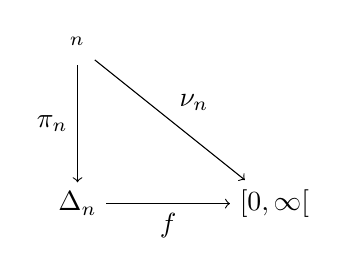
\begin{tikzpicture}[auto]
  \node (A)  at (0,0) {$\RR^n$};
  \node (C)  at (0,-2) {$\Delta_n$};
  \node (D)  at (2.5,-2) {$[0,\infty[$};
  \draw[->] (A) to node [swap] {$\pi_n$} (C);
  \draw[->] (C) to node [swap] {$f$} (D);
  \draw[->] (A) to node  {$\nu_n$} (D);
\end{tikzpicture}
\end{center}

\alinea{2)} Let us denote by $0_k$ the zero of $\RR^k$. Next, let us assume that
the plot $\nu_n$ can be lifted at the point $0_n$ along a $p$-plot 
$\P : \U \to \Delta_n$, with $p < n$. Let $\phi : \V \to \U$ be a smooth
parametrization  such that $\P \circ \phi = \nu_n
  \restriction \V$. We can assume without loss of generality that
$\P(0_p) = 0$ and $\phi(0_n) = 0_p$. If it is not the case we compose
$\P$ with a translation mapping $\phi(0_n)$ to $0_p$. Now, since $\P$
is a plot of $\Delta_n$, it can be lifted locally at the point $0_p$
along $\nu_n$. Let $\psi : \W \to \RR^n$ be a smooth parametrization 
 such that $0_p \in \W$ and $\nu_n \circ \psi = \P
    \restriction \W$. Let us introduce $\V' = \phi^{-1}(\W)$, we have then the
following commutative diagram.
    \begin{center}
  \begin{tikzpicture}
  \node (A)  at (3,0) {$\W$};
  \node (B)  at (0,-3) {$V'$};
  \node (C)  at (3,-3) {$[0,\infty[$};
  \node (D)  at (6,-3) {$\RR^n$};
  \draw[->] (B) to node [auto] {$\phi \restriction \V'$} (A);
  \draw[->] (B) to node [auto,swap] {$\nu_n \restriction \V'$} (C);
  \draw[->] (A) to node [fill=white] {$\P \restriction \W$} (C);
  \draw[->] (A) to node [auto] {$\psi$} (D);
  \draw[->] (D) to node [auto] {$\nu_n$} (C);
  \end{tikzpicture}
    \end{center}
Now, denoting by $\F = \psi \circ \phi
  \restriction \V'$, we get $\nu_n \restriction \V' = \nu_n \circ \F$,
with $\F \in \Cinfty(\V', \RR^n)$, $0_n \in \V'$ and $\F(0_n) = 0_n$,
that is,
$$
  \norm{x}^2 = \norm{\F(x)}^2.
  $$
The derivative of this identity gives 
$$
  x \cdot \delta x =  \F(x) \cdot \D(\F)(x)(\delta x),
  \mbox{ for all } x \in \V' \mbox{ and for all } \delta x \in \RR^n.
  $$
The second derivative, computed at the point $0_n$, where $\F$
vanishes, gives then
$$
  \id_n = \M^t \M \qmbox{with} \M = \D(\F)(0_n),
  $$
where $\M^t$ is the transposed matrix of $\M$. But $\D(\F)(0_n)
  = \D(\psi)(0_p) \circ \D(\phi)(0_n)$. Let us denote $\A =
    \D(\psi)(0_p)$  and $\B = \D(\phi)(0_n)$, $\A \in \Lin(\RR^p, \RR^n)$
and $\B \in \Lin(\RR^n, \RR^p)$. Thus $\M = \A \B$ and the previous
identity $\id_n = \M^t \M$ becomes 
$\id_n = \B^t \A^t \A \B$. But the rank of $\B$ is less or equal to $p$ which
is, by hypothesis, strictly less than $n$, which would imply that the
rank of $\id_n$ is strictly less than $n$. And this is not true: 
the rank of $\id_n$ is $n$. Therefore, the plot $\nu_n$
cannot be lifted locally at the point $0_n$ by a $p$-plot of $\Delta_n$
with $p < n$.

\alinea{3)} The diffeology of $\Delta_n$, represented by $(\left[0, \infty
  \right[, \cD_n)$, is generated by $\nu_n$. Hence, $\cF = \set{\nu_n}$ is
a generating family for $\Delta_n$. Therefore, by definition of the
dimension of diffeological spaces
\art{Dimension-of-a-diffeological-space}, 
$\dim(\Delta_n) \leq n$. Let us assume that
$\dim(\Delta_n) = p$ with $p < n$. Then, since $\nu_n$ is
a plot of $\Delta_n$ it can be lifted locally, at the
point $0_n$, along an element $\P'$ of some generating
family $\cF'$ for $\Delta_n$. The family $\cF'$
satisfies $\dim(\cF') = p$. But, by definition of the
dimension of generating families
\art{Dimension-of-a-family-of-parametrizations}, we get
$\dim(\P') \leq p$, that is, $\dim(\P') < n$. This is
not possible, thanks to second question. Therefore,
$\dim(\Delta_n) = n$. Now, since the dimension is a
diffeological invariant
\art{The-dimension-is-a-diffeological-invariant},
$\Delta_n = \RR^n / \OG(n, \RR)$ is not diffeomorphic to
$\Delta_m = \RR^m / \OG(m, \RR)$ when $n \neq m$.
\endsolexref

\solexref{Dimension-of-the-half-line}
(Dimension of the half-line)
First of all, let us remark that all the maps 
$\nu_n : \RR^n \to \Delta_\infty$, defined by $\nu_n(x) = \norm{x}^2$, are plots of
$\Delta_\infty$. Indeed, these $\nu_n$ are smooth parametrizations of $\RR$ and
take their values in $\left[0, \infty \right[$. Now, let us assume that
$\dim(\Delta_\infty) = \N < \infty$. Hence for any integer $n$, the plot
$\nu_n$ lifts locally at the point $0_n$ along some $p$-plot of
$\Delta_\infty$, with $p \leq \N$. Let us choose now
$n > \N$. Then, there exist a smooth parametrization $f : \U \to \RR$
such that $\Val(f) \subset \left[0, \infty \right[$,
that is, $f$ is a $p$-plot of $\Delta_\infty$, and a smooth
parametrization $\phi : \V \to \U$ such that 
$f \circ \phi = \nu_n \restriction \V$.  
\begin{center}
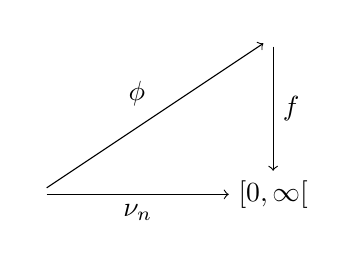
\begin{tikzpicture}[auto]
  \node (B)  at (3,0) {$\U$};
  \node (C)  at (0,-2) {$\V$};
  \node (D)  at (3,-2) {$[0,\infty[$};
  \draw[->] (C) to node {$\phi$} (B);
  \draw[->] (C) to node [swap] {$\nu_n \restriction \V$} (D);
  \draw[->] (B) to node {$f$} (D);
\end{tikzpicture}
\end{center}
We can assume, without loss of
generality, that $0_p \in \U$, $\phi(0_n) = 0_p$, which implies
$f(0_p) = 0$. Now, let us follow the method of
\exref{Dimension-of-Rn/On}. The first derivative of $\nu_n$ at a point
$x \in \V' = \phi^{-1}(\V)$ is given by: $$ x =  \D(f)(\phi(x)) \circ
  \D(\phi)(x).
  $$
Since $f$ is smooth, positive, and $f(0)=0$, we have in particular
$\D(f)(0_p) = 0$. Now, considering this property, the second
derivative, computed at the point $0_n$, gives in matricial notation:
$$ 
\id_n = \M^t \H \M, \mbox{ where } \M = \D(\phi)(0) \mbox{ and } \H = \D^2(f)(0), 
$$ 
where $\M^t$ is $\M$ transposed, and $\H$ is the Hessian of $\phi$ 
at the point $0_n$, a symmetric bilinear map. The matrix $\M$
represents the tangent map of $f$ at $0_p$. Now, since we chose 
$n > \N$ and assumed $p \leq \N$, we have $p < n$. Thus the map $\M$ has
a non zero kernel and then $\M^t \H \M$ is degenerate, which is
impossible since $\id_n$ is nondegenerate. 
Therefore, the dimension of $\Delta_\infty$ is unbounded, that is, infinite.
\endsolexref

%%%%%%%%%%%%%%%%%%%%%%%%%%%%%%%%%%%%%%%%%%%%%%%%%%%%%%%%%%
%% 
%% Local differentiablity
%% 
%%%%%%%%%%%%%%%%%%%%%%%%%%%%%%%%%%%%%%%%%%%%%%%%%%%%%%%%%%
\SkipTocEntry\section*{Locality and Diffeologies}

\solexref{To-be-a-locally-constant-map}
(To be a locally constant map)
Let $\gamma \in \Cinfty(\RR,\X)$ with $\gamma(0)= x_0$ and $\gamma(1)= x_1$.
For all $t \in [0,1]$ there exists a superset $\V_t$ of $\gamma(t)$ such that
$f \restriction \V_t$ is a local smooth map, according to the definition 
\art{Local-smooth-maps}. In particular $\cI_t = \gamma^{-1}(\V_t)$ is a $1$-domain 
containing $t$ and it satisfies $f(\gamma(\cI_t)) = \const$. The $\cI_t$ are a covering 
of the segment $[0,1]$ which is compact. Then, adapting the arguments of
\exref{Locally-constant-parametrizations} to $f \circ \gamma$, we get $f(x_0) = f(x_1)$.
Therefore, $f$ is constant on the connected components of $\X$.

\endsolexref

%%%%%%%%%%%%%%%%%%%%%%%%%%%%%%%%%%%%%%%%%%%%%%%%%%%%%%%%%%
%% 
%% D-topology and local smoothness
%% 
%%%%%%%%%%%%%%%%%%%%%%%%%%%%%%%%%%%%%%%%%%%%%%%%%%%%%%%%%%
\SkipTocEntry\section*{D-Topology and Local Smoothness}

\solexref{Diffeomorphisms-of-the-square}
(Diffeomorphisms of the square)
A diffeomorphism from the square must send corner into corner, because 
every smooth map into a corner must be flat, \exref{Smooth-injection-in-the-corner},
which is not the case for the other points of the square. Thus, we can associate
with every diffeomorphism $\varphi$ of the square a permutation $\sigma = h(\varphi)$ of the 
set of four corners. The map $h$ is clearly a homomorphism.
But $\varphi$ is a diffeomorphism which also permutes 
the edges of the square in a coherent way with $\sigma$, the image of
connected edges to a corner must be connected to the image of this corner. 
Eventually, the image of $h$ is  the dihedral
group with eight elements, generated by the rotation of angle $\pi/4$
and a reflection by an axis of symmetry.

\endsolexref

\solexref{Smooth-D-topology}
(Smooth D-topology)
Let $\U \subset \RR^n$ be a domain, that is, an ordinary open subset of
$\RR^n$. Let
${\A}\subset {\U}$ be open in
${\U}$, that is,
${\A}$ open in
$\RR^n$. Let ${\P}: {\V} \to {\U}$ be a plot of ${\U}$, that is, any
smooth parametrization. Since smooth parametrizations
are continuous maps for the standard topology, the pullback
${\P}^{-1}({\A})$ is open. Then, any open set of ${\U}$, for the usual
topology, is D-open. Conversely, let ${\A}\subset {\U}$ be D-open, the
identity map
$\id_ {\U}$ being a plot of ${\U}$, the subset $\id_ {\U}^{-1}({\A}) =
  {\A}$ is open. Then, any D-open set of
${\U}$ is open for the usual topology. Thus, the standard topology
and the D-topology of smooth domains coincide. 
\endsolexref

\solexref{D-topology-of-irrational-tori}
(D-topology of irrational tori)
Let $\pi: \RR \to \T_\Gamma$ be the natural projection. The set
$\T_\Gamma$ is equipped with the quotient diffeology
\art{Quotient-and-quotient-diffeology}. Let
${\A}\subset {\T}_{\Gamma}$ be a non-empty D-open. Since the projection
$\pi$ is smooth, it is D-continuous 
\art{Smooth-maps-are-D-continuous}. Thus,
$\pi^{-1}({\A})$ is a D-open in $\RR$, that is, 
$\pi^{-1}({\A})$ is a domain
(\exref{Smooth-D-topology}). Let $\tau \in {\A}$ and $x
  \in \RR$ such that $\pi(x) = \tau$. So, $\pi^{-1}({\A})$
contains $x$ and its whole orbit by the action of
$\Gamma$. Let us denote by $\cO$ this orbit, thus
$\pi^{-1}({\A})$ is an open neighborhood of $\cO$. But
$\Gamma$ being dense in $\RR$, the orbit $\cO$ also is
dense, and $\pi^{-1}({\A})$ is an open neighborhood of a
dense subset of $\RR$. Therefore, $\pi^{-1}({\A}) = \RR$
and ${\A} = {\T}_{\Gamma}$. Therefore, the only non-empty
D-open set of ${\T}_{\Gamma}$ is ${\T}_{\Gamma}$ itself.
The D-topology of ${\T}_{\Gamma}$ is coarse.
%
Now, a full functor is a functor surjective on the arrows \cite{McL71}.
Since the D-topology of $\T_\Gamma$ is coarse, any map from $\T_\Gamma$
to $\T_\Gamma$ is D-continuous. But we know by
\exref{Smooth-maps-on-R/Q} that all maps from $\T_\QQ$
to $\T_\QQ$ are not smooth, just the affine ones. Hence the D-topology
functor is not surjective on the arrows, that is, not full. 
\endsolexref

%%%%%%%%%%%%%%%%%%%%%%%%%%%%%%%%%%%%%%%%%%%%%%%%%%%%%%%%%%
%% 
%% Embeddings and embedded parts
%% 
%%%%%%%%%%%%%%%%%%%%%%%%%%%%%%%%%%%%%%%%%%%%%%%%%%%%%%%%%%
\SkipTocEntry\section*{Embeddings and Embedded Subsets}

\solexref{Q-is-discrete-but-not-embedded-in-R}
($\QQ$ is discrete but not embedded in $\RR$)
Let us recall that $\QQ$ is discrete in $\RR$
\art{Diffeology-of-Q-in-R}, that is, the subset diffeology is discrete.
The D-topology of
$\RR$ is the smooth topology \art{Smooth-D-topology} and, since
$\QQ\subset \RR$ is discrete, the D-topology of $\QQ$ is discrete
\art{D-topology-on-discrete-and-coarse-diffeological-spaces}. But,
since any non empty open set of the topology induced by $\RR$ on $\QQ$ contains
always an infinite number of points (it is generated by the
intersections of open intervals and $\QQ$), the induced D-topology is
not discrete. Then, $\QQ$ is not embedded in $\RR$.
\endsolexref

\solexref{Embedding-GL-n-R-in-Diff-R-n}
(Embedding $\GL(n,\RR)$ in $\Diff(\RR^n)$)
\newcommand{\Pij}{\P_{ij}}
Let us recall that the plots of the functional diffeology of
$\Diff(\RR^n)$ 
\art{Functional-diffeology-on-groups-of-diffeomorphisms} are
the parametrizations $\P : \U \to \Diff(\RR^n)$ such that
$$
  [(r,x) \mapsto \P(r)(x)] \mbox{ and }  [(r,x) \mapsto \P(r)^{-1}(x)]
  \mbox{ belong to } \Cinfty(\U
  \times \RR^{n},\RR^{n}).
  $$
  
\alinea{1)} The diffeology of $\GL(n,\RR)$ induced by $\Diff(\RR^n)$ coincides
with the ordinary diffeology. 

\alinea{}The plots of the standard diffeology of $\GL(n,\RR)$ are the
parametrizations $\P : \U \to \GL(n,\RR)$ such that every component
$\Pij$ is smooth, that is, 
$$
  \Pij : r \mapsto \left\langle \ee_{j} \mid \P(r)(\ee_{i}\,)\right\rangle \in
  \Cinfty(\U,\RR), \ \mbox{for all} \ i,j = 1, \ldots, n,
  $$
where we have denoted by $\ee_1, \ldots , \ee_n$ the vectors of
the canonical basis of $\RR^{n}$, and by $\left\langle\cdot\mid\cdot\right\rangle$ the
ordinary scalar product of $\RR^n$.
%
Now, for each $(r,x) \in \U\times \RR^n$,
$\P(r)(x) = \P(r)(\sum_{i=1}^n x^i \ee_i) = \sum_{i=1}^n
  x^i \P(r)(\ee_i) = \sum_{i=1}^n x^i \Pij(r) \ee_j$. If all the
components $\Pij$ of the parametrization $\P$ are smooth, then $(r,x)
  \mapsto \sum_{i=1}^n x^i \Pij(r)
  \ee_j$ is smooth, and the map $(r,x) \mapsto \P(r)(x)$ is smooth. Since
the determinant of $\P(r)$ never vanishes, the same holds for $(r,x)
  \mapsto \P(r)^{-1}(x)$. Therefore,
$\P$ is a plot of the functional diffeology. 
%
Conversely, if $\P$ is a plot of the functional diffeology --- that is,
the parametrization
$(r,x)\mapsto \P(r)(x)$ is smooth --- then, restricting this
map to $x = \ee_i$, we get that the map $r \mapsto \P(r)(\ee_i) =
  \sum_{j=1}^n
  \Pij(r)
  \ee_i$ is smooth. So, by contracting this parametrization to the
vector $\ee_j$, we get that all the matrix components $\Pij$ are smooth.
Thus, the inclusion
$\GL(n,\RR) \hookrightarrow \Diff(\RR^n)$ is an induction.

\alinea{2)} The inclusion $\GL(n,\RR) \hookrightarrow \Diff(\RR^n)$ is an
embedding.

\alinea{}We have to show that the topology of
$\GL(n,\RR)$ induced by the D-topology of $\Diff(\RR^n)$
coincides with the D-topology of $\GL(n,\RR)$, that is, the topology
induced by its inclusion into $\RR^{n \times n}$. 
%
Let $\B({\bf 1}_{n},
  \varepsilon)$ be the open ball in $\GL(n,\RR)$ centered at the identity
${\bf 1}_{n}$, with radius $\varepsilon$. Let $\Omega_{\varepsilon}$ be
the set of all diffeomorphisms defined by
%
\begin{displaymath}
  \Omega_{\varepsilon} = \{f\in \Diff(\RR^{n}) \mid \D (f)(0)\in \B({\bf
  1}_{n}, \varepsilon) \},
\end{displaymath}
%
where $\D(f)(0)$ is the tangent linear map of
$f$ at the point $0$. Now, let us prove the following.

\alinea{a)} The set $\Omega_{\varepsilon}$ is open
for the D-topology of $\Diff(\RR^{n})$.

\alinea{}Let $\P : \U \rightarrow \Diff(\RR^{n})$ be a plot, that is,
$[(r,x)\mapsto \P(r)(x)]\in
  \Cinfty(\U \times \RR^{n},\RR^{n})$. The pullback of
$\Omega_{\varepsilon}$ by
$\P$ is the set of $r \in \U$ such that the tangent map
$\D(\P(r))(0)$ is in the ball $\B({\bf 1}_{n}, \varepsilon)$, formally,
$$
  \P^{-1}(\Omega_{\varepsilon}) = \{ r\in \U \mid \D(\P(r))(0)
  \in \B({\bf 1}_{n},
  \varepsilon) \}.
  $$
Considering $\P$ as a smooth map
defined on
$\U \times
  \RR^{n}$,
$\D(\P(r))(0)$ is the partial derivative of $\P$, with respect to
the second variable, computed at the point $x=0$. 
The map $[r \mapsto \D(\P(r))(0)]$ is then continuous, by
definition of smoothness. Hence, the pullback of
$\Omega_{\varepsilon}$ by this map is open. Because
the imprint of this open set on 
$\GL(n,\RR)$ is exactly the ball
$\B({\bf 1}_{n}, \varepsilon)$, we deduce that any open ball of 
$\GL(n,\RR)$ centered at ${\bf 1}_{n}$ is the imprint of a
D-open set of $\Diff(\RR^{n})$. 

\alinea{b)} Every open of $\GL(n,\RR)$ is the imprint of a D-open set of
$\Diff(\RR^n)$.

\alinea{}By using the group operation on $\GL(n,\RR)$ and since any open set of
$\GL(n,\RR)$ is a union of open balls, every
open subset of $\GL(n,\RR)$ is the imprint of some D-open subset of
$\Diff(\RR^n)$. Therefore, $\GL(n,\RR)$ is embedded in $\Diff(\RR^{n})$. 
\endsolexref

\solexref{The-irrational-solenoid-is-not-embedded}
(The irrational solenoid is not embedded)
The solenoid is the subgroup 
$[\alpha] = \{(1,e^{i2\pi\alpha t}) \mid t \in \RR\} \subset \Torus^2$, with
$\alpha \in \RR-\QQ$. It is the image of the induction $j : t \mapsto (1,e^{i2\pi\alpha t})$,
from $\RR$ to $\Torus^2$, \exref{The-irrational-solenoid}. Because $[\alpha]$ is dense in $\Torus^2$, the pullback
of any open disc of $\Torus^2$ by $j$ is an infinite disjoint 
union of intervals of $\RR$. Thus, an open interval 
$\openinterval{a,b} \subset \RR$ cannot be the preimage of an open
subset of $\Torus^2$. Therefore, the solenoid is not embedded in $\Torus^2$.
\endsolexref


%%%%%%%%%%%%%%%%%%%%%%%%%%%%%%%%%%%%%%%%%%%%%%%%%%%%%%%%%%
%% 
%% Local or weak inductions
%% 
%%%%%%%%%%%%%%%%%%%%%%%%%%%%%%%%%%%%%%%%%%%%%%%%%%%%%%%%%%
\SkipTocEntry\section*{Local or Weak Inductions}

\solexref{The-infinite-symbol}
(The infinite symbol)
1) If $j(t) = j(t')$, $t \neq t'$, and $t,t' \in ]-\pi, \pi[$, then 
$t'-t = \pm \pi/2$ and  $t'-t = \pm \pi/4$. Thus, $t =t'$ and thus the map $j$ is
injective.

\alinea{2)} The drawing of $\P$ (fig. \ref{theplotP}) clearly shows 
that $j$ and $\P$ have the same image in $\RR^2$. But the precize reason
is given by ($\clubsuit$) in 3).

%%###########
\begin{figure}[tb]
  \centerline{\includegraphics{Figures-PDF/fig-P.pdf}}
  \caption{The plot ${\P}$.}\label{theplotP}
\end{figure}
%%###########

\alinea{3)} Comparing the figure of $j$ and the figure of $\P$, we see clearly that 
$$j^{-1} \circ {\P}(]-\pi/4,\pi/4[) = \, ]-\pi,-3\pi/4[
  \ \cup \ \{0\}
  \ \cup \ 
  ]3\pi/4,\pi[.
  $$
The map $j^{-1} \circ {\P}$ has a continuity gap at $t = 0$, so
$j^{-1} \circ {\P}$ is not continuous, {\em a fortiori\/} not
smooth. But, we have precisely: 
\begin{equation}
  \renewcommand{\theequation}{$\clubsuit$}
  j^{-1} \circ {\P}(t) = \left\{
  \begin{array}{ll}
    -t -\pi & \ t \in ]-\pi/4,0[ \\
    0 & \ t = 0 \\
    -t +\pi & \ t\in]0,\pi/4[
  \end{array}
  \right..
\end{equation}
Hence, $\P$ is a plot of $\RR^2$ with values in $j(]-\pi,\pi[)$, but
$j^{-1} \circ \P$ is not smooth. Therefore, by application
of \art{Criterion-for-being-an-induction},  the injection $j$ is not an
induction.

\alinea{4)} The map $j$ is an immersion, its derivative never vanishes on 
 $]-\pi, \pi[$. Thus, as an application of the \exref{Immersions-of-real-domains},
 it is a local induction everywhere.
\endsolexref


%%%%%%%%%%%%%%%%%%%%%%%%%%%%%%%%%%%%%%%%%%%%%%%%%%%%%%%%%%
%% 
%% Local or strong subductions
%% 
%%%%%%%%%%%%%%%%%%%%%%%%%%%%%%%%%%%%%%%%%%%%%%%%%%%%%%%%%%
\SkipTocEntry\section*{Local or Strong Subductions}

\solexref{Quotient-by-a-group-of-diffeomorphisms}
(Quotient by a group of diffeomorphisms)
1) Let $\P : \U \to \cQ$ be a plot. By definition of the quotient
diffeology of $\G/\pi$, for all $r_0 \in \U$ there exist an open neighborhood
$\V$ of $r_0$ and a plot $\gamma : \V \to \G$ such that 
$\P(r) = \gamma(r)(x)$ for all $r \in \V$. Hence, 
$\P \restriction \V = [r \mapsto (r,x) \mapsto \gamma(r)(x)]$, 
but $[r \mapsto (r,x)]$ is clearly  smooth, and 
$[(r,x) \mapsto \gamma(r)(x)]$ 
is smooth by the very definition of the functional diffeology. 
Thus, $\P \restriction \V$ is a plot of the subset diffeology. 
Therefore $j$ is smooth. The quotient diffeology of $\G(x)$ is finer than its subset
diffeology.

\alinea{2)} Let $\P : \U \to \cQ$ be a plot, let $r \in \U$ and $g \in \G$ 
such that $\pi(g) = \P(r)$, that is, $g(x) = \P(r)$. 
By definition of the quotient diffeology there exist an open neighborhood 
$\V$ of $r$ and a plot $\gamma : \V \to \G$ such that 
$\P \restriction \V = \pi \circ \gamma$. Let $g' = \gamma(r)$, 
then $\pi(g') = \pi(g) = \P(r)$, that is, $g(x) = g'(x)$ or  $g'^{-1}(g(x)) = x$.  
Now, let us define on $\V$,
$\gamma' = [s \mapsto \gamma(s) \circ g'^{-1} \circ g]$. 
On the one hand, we have $\gamma'(s)(x) = \gamma(s)(g'^{-1}(g(x)))$, 
but $g'^{-1}(g(x)) = x$, thus $\gamma'(s)(x) = \gamma(s)(x)$, 
that is, $\pi \circ \gamma' = \pi \circ \gamma = \P \restriction \V$. 
On the other hand we have $\gamma'(r) = \gamma(r) \circ g'^{-1} \circ g$, 
but $g' = \gamma(r)$, thus $\gamma'(r) = g$. Since, by definition of the functional
diffeology of $\G$ \art{Functional-diffeology-on-groups-of-diffeomorphisms}, 
composition and inversion are smooth, the parametrization $\gamma'$ is a plot of
$\G$. Moreover, $\gamma'$ satisfies the conditions
$\P \restriction \V = \pi \circ \gamma'$ and $\gamma'(r) = g$. 
Therefore $\pi$ is a local subduction.

\alinea{3)} By definition of generating families \art{Generating-diffeology}, a plot $\P$
of the Tahar rug $\cT$ writes locally $[r \mapsto (t(r),c)]$ or 
$[r \mapsto (c,t(r))]$, where $c$ is some constant and $t$ is a
smooth real function. Now, let $u =(a,b) \in \RR^2$, 
the composition $\T_u \circ \P$ writes locally either $[r \mapsto (t'(r),c')]$,
with $t'(r) = t(r) +a$ and $c' = c+b$, or $[r \mapsto (c',t'(r))]$, with 
$t'(r) = t(r) + b$ and $c' = c + a$. Thus, $\T_u$ is smooth. Then, since
$(\T_u)^{-1} = \T_{-u}$, $\T_u$ is a diffeomorphism of $\cT$. Now, let 
$r \mapsto u(r) =(a(r),b(r))$ be a parametrization of $\RR^2$ 
such that $r \mapsto \T_{u(r)}$ is a plot for the functional diffeology. 
Composed with the 1-plots $t \mapsto (t,c)$, where $c$ runs over $\RR$, we must get a 
plot $(r,t) \mapsto (t + a(r), c+b(r))$ of $\cT$, that is, a plot which is locally 
of the first or the second kind. Hence, either $(r,t) \mapsto t + a(r)$ 
is locally constant, or $(r,t) \mapsto c + b(r)$. But $(r,t) \mapsto t + a(r)$ 
is not locally constant because of its dependency on $t$, thus 
$(r,t) \mapsto c + b(r)$ is locally constant, that is, $b(r) =_\loc b$, for some
$b \in \RR$. In the same way, composing with the 1-plots $t \mapsto (c,t)$, 
we get that $a(r) =_\loc a$. Therefore, $r \mapsto \T_{u(r)}$ is locally constant,
that is, the group of translations, equipped with the functional diffeology, is discrete.
Finally, the action of the translations on $\cT$ is free, the orbit of $(0,0)$ is
$\cT$, and since the diffeology of $\cT$ is not the discrete diffeology, we get 
an example, for the first question, where the diffeology of $\cQ$ is strictly 
finer than the one of $\cO$.
\endsolexref

\solexref{A-not-so-strong-subduction}
(A not so strong subduction)
As an application of \art{Uniqueness-of-quotient}, the underlying set of
$\cQ$ can be represented by the half line $[0,\infty[$ equipped with
the image of the diffeology of
$\RR\coprod\RR^2$ by the map $p: x \mapsto \norm{x}^2$.
%%###########
\begin{figure}[tb]
  \centerline{\includegraphics{Figures-PDF/fig-R1R2.pdf}}
  \caption{The quotient $\cQ$}\label{quotientR1R2}
\end{figure}
%%###########
Let $0$ and $(0,0)$ be the zeros of $\RR$ and 
$\RR^2$, and let $\P$ be the plot $p\restriction \RR^2$. 
Then, $\P(0,0) = 0 \in[0,\infty[$. Let us assume now that $\P$
lifts locally at $(0,0)$ along $p$, by a plot $f$ such that $f(0,0) = 0$. 
Thus, $f$ takes its values in $\RR$ and $p \circ f = \P$, that is, 
$f(a,b)^2 = a^2+b^2$, at least locally. 
Since $f$ is continuous and vanishes only at $(0,0)$, and
since the complementary of $(0,0)$ in $\RR^2$ is connected, $f$
keeps a constant sign, thus $f(a,b) = \pm \sqrt{a^2+b^2}$. But none of
these two cases is smooth at $(0,0)$. Therefore,
$p$ is not a local subduction at the point $0$.
\endsolexref

\solexref{A-powerset-diffeology}
(A powerset diffeology) 
1) Let us check that the param\-etrizations 
defined by ($\clubsuit$) are a diffeology.

\alinea{D1.} Let $\P : \U \to \Powerset(\X)$ be the constant
parametrization $r \mapsto \A \subset \X$. Let 
$r_0 \in \U$, let $\Q_0 \in \cD$ such that 
$\Val(\Q_0) \subset \A = \P(r_0) = \P(r)$ for all $r \in \U$. 
Let $\Q : \U \to \cD$ given by $\Q(r) = \Q_0$, for all $r \in \cD$.
This is a constant family of plots of $\X$, hence smooth. 
Thus, $\P$ satisfies the condition ($\clubsuit$). Hence, the
constant parametrizations satisfy ($\clubsuit$).

\alinea{D2.} The locality axiom is satisfied by
construction: ($\clubsuit$) is a local
property. 

\alinea{D3.} Let us consider a parametrization 
$\P : \U \to \Powerset(\X)$ satisfying ($\clubsuit$). 
Let $\F : \U' \to \U$ be a smooth parametrization. 
Let $\P' = \P \circ \F$. Let $r'_0 \in \U'$ and $r_0 = \F(r'_0)$. 
By hypothesis, for every $\Q_0 \in \cD$ such
that $\Val(\Q_0) \subset \P(r_0) = \P'(r'_0)$, there
exist an open neighborhood $\V$ of $r_0$ and a smooth family of plots
$\Q : \V \to \cD$ such that $\Q(r_0) = \Q_0$ and 
$\Val(\Q(r)) \subset \P(r)$, for all $r \in \V$. 
Let us then define $\V' = \F^{-1}(\V)$ and $\Q' = \Q \circ \F$.
Since $\F$ is smooth, $\V'$ is a domain, and since $\Q$ is a
smooth family of plots, so is $\Q \circ \F$. Thus, for
every $r'_0 \in \U'$, for every $\Q_0 \in \cD$ such that 
$\Val(\Q_0) \subset \P'(r'_0)$, we found a smooth family of plots $\Q'$ 
such that $\Q'(r'_0) = \Q(r_0) = \Q_0$ and 
$\Val(\Q'(r')) = \Val(\Q \circ \F(r')) = \Val(\Q(r)) \subset \P(r) = \P'(r')$, 
where $r = \F(r')$. Therefore, $\P' = \P \circ \F$ satisfies ($\clubsuit$).

\alinea{2)} Consider now the relation $\cR$ from $\Powerset(\X)$ to 
$\cD$ defined by the inclusion
$$
 \cR = \{ (\A,\Q) \in \Powerset(\X) \times \cD \mid \Val(\Q) \subset \A \}.
$$
Let $\P : \U \to \Powerset(\X)$
be a parametrization regarded as the relation 
$$
\P = \{(r,\A) \in \U \times  \Powerset(\X) \mid \A = \P(r) \}.
$$
The composite $\cR \circ \P$, also denoted by $\P^*(\cR)$, is then given by
$$
 \P^*(\cR) = \{ (r, \Q) \in \U \times \cD \mid \Val(\Q) \subset \P(r) \}.
$$
The parametrization $\P$ is a plot of the powerset diffeology if and only if
the first projection $\pr_1 : \P^*(\cR) \to \U$ is everywhere a local subduction.
Now, if $f : \X \to \Y$ is a map between two diffeological spaces, $f$ is smooth
if and only if the first projection from $\bmf = \{(x,y) \in \X \times \Y \mid y = f(x) \}$
to $\X$ is a subduction, which is equivalent to be a local subduction, in this case. 
%
Note that this construction gives an idea of what can be a {\em smooth relation}
from a diffeological space $\X$ to another $\X'$. 
Indeed, let $\cR \subset \X \times \X'$ be a relation from $\X$ to $\X'$, we 
declare $\cR$ smooth if for every plot $\P$ in $\Dom(\cR) = \pr_1(\cR) \subset \X$,
for every $r \in \U$ and every $(\P(r),x') \in \cR$, there exists a plot 
$\Q : \V \to \X'$, with $\V \subset \U$, such that $(\P(r'),\Q(r')) \in \cR$ 
for all $r' \in \V$ and $\Q(r) = x'$. In other words, $\pr_1 : \cR \to \Dom(\cR)$
is a local subduction everywhere, where $\cR$ and  $\Dom(\cR)$ are equipped with
the subset diffeology. 
%
With this terminology, back to the powerset diffeology, 
a parametrization $\P : \U \to \Powerset(\X)$
is a plot if the composite $\cR \circ \P$ is a smooth relation from $\U$ to 
$\cD$.

\alinea{3)} Let us check now that the map $j : x \mapsto \set{x}$ 
is an induction.
We consider the criterion for \art{Criterion-for-being-an-induction}. 
First of all let us remark that $j$ in injective. Next, let us check that
the map $j$ is smooth. Let $\P : \U \to \X$ be a plot.
Thus, $j \circ \P(r) = \set{\P(r)}$. Let $r_0 \in \U$ and
$\Q_0 \in \cD$ such that 
$\Val(\Q_0) \subset j \circ \P(r_0) = \set{\P(r_0)}$. 
So, $\Val(\Q_0)$ is the point $\P(r_0)$ of $\X$, that is,
$\Q_0$ is the constant plot $s \mapsto \P(r_0)$. Let us
then define, for every $r \in \U$, $\Q(r)$ as the
constant plot 
$[s \mapsto \P(r)]$, with $\Dom(\Q(r)) = \Dom(\Q_0)$. 
Since, for every $r \in \U$, the parametrization 
$[(r,s) \mapsto \Q(r)(s) = \P(r)]$, defined on $\U \times \Dom(\Q_0)$,
is clearly a plot of $\X$, then $\Q$ is a smooth family of plots of $\X$. 
Therefore, $j \circ \P$ is a plot of $\Powerset(\X)$, and $j$ is
smooth.
%
Then, let us check that the map $j^{-1} : j(\X) \to \X$
is smooth. Let $\P : \U \to j(\X)$ be a plot of the
powerset diffeology. First of all, for every $r \in \U$
there exists a unique point $q(r) \in \X$ such that 
$\P(r) = \set{q(r)}$. Then, since $\P$
is a plot of $\Powerset(\X)$, for all
$r_0 \in \U$, for every plot $\Q_0$ of $\X$ such that
$\Val(\Q_0) \subset \P(r_0) = \set{q(r_0)}$, there
exist an open neighborhood $\V$ of
$r_0$, and a smooth family of plots $\Q$ of $\X$, such that 
$\Val(\Q(r)) \subset \P(r)$, for all $r \in \V$. Then, let us choose the $0$-plot
$\Q_0 : \RR^0 \to \X$, with $\Q_0(0) = q(r_0)$, that is, $\Val(\Q_0) = \P(r_0)$. 
Thus, $\Q$ is necessarily a smooth family of $0$-plots 
(see \art{Functional-diffeology-of-a-diffeology}).
But $\Val(\Q(r)) \subset \P(r) = \set{q(r)}$ 
means exactly that $\Q(r)(0) = q(r)$. Hence, 
$q \restriction \V = [r \mapsto \Q(r)(0)]$ is a plot of $\X$. 
Therefore, $q = j^{-1} \circ \P$ is a plot of $\X$, and $j^{-1}$ is
smooth.
Finally, thanks to the criterion
\art{Criterion-for-being-an-induction}, $j$ is an
induction from $\X$ into $\Powerset(\X)$.

\alinea{4)} Let us show, now, that the Tzim-Tzum $\cT$ is a plot of the 
powerset diffeology of $\Powerset(\RR^2)$. Let $t_0 \in\RR$ and consider
$\cT_{t_0}$. Let $\Q_0 : \U \to \cT_{t_0}$ be a plot. If $t_0 < 0$,
then we can choose $\Q(t)(r) = \Q_0(r)$ for 
$t \in \openinterval{3t_0/2,t_0/2}$. $\Q$ is a smooth family of plots of 
$\RR^2$ such that $\Q(t_0) = \Q_0$ and $\Val(\Q(t)) \subset \cT(t) = \RR^2$. 
For $t_0= 0$, we choose $\Q(t)(r) = (e^t + t/\norm{\Q_0(r)})\Q_0(r)$. Since 
$\cT(0) = \RR^2-\{0\}$, $\Q_0(r) \neq 0$ for all $r$, 
$\Q(t)$ is well defined and $\Q$ is a smooth 
family of plots of $\RR^2$. Next, note first that $\Q(0) = \Q_0$. Then, 
for $t \geq 0$, $\norm{\Q(t)(r)} = t + e^t \norm{\Q_0(r)} > t$, since
$\norm{\Q_0(r)} > 0$, thus $\Val(\Q(t)) \subset \cT(t)$. For $t <0$ there is
nothing to check since $\cT(t) = \RR^2$. Now, if $t_0 > 0$, we can choose 
$\Q(t)(r) = [1 + (t-t_0)/t_0]\Q_0(r)$. We have $\Q(t_0) = \Q_0$, then
$\norm{\Q(t)(r)} = \vert 1 + (t-t_0)/t_0 \vert \norm{\Q_0(r)}$. But,
$\norm{\Q_0(r)} > t_0$ implies 
$\norm{\Q(t)(r)} > \vert 1 + (t-t_0)/t_0 \vert t_0 = \vert t \vert$. 
Thus, if $t \geq 0$, then $\norm{\Q(t)(r)} > t$, for all $r$, that is, 
$\Val(\Q(t)) \subset \cT(t)$. 
We exhausted all the cases, and therefore $\cT$ is a plot of the 
powerset diffeology of $\Powerset(\RR^2)$. 
As we  can see, there is a blowing up for $t = 0$, 
the space opens up, an empty bubble appears and grows with it. 
This is the reason for which we named this plot Tzim-Tzum. 
\endsolexref

\solexref{The-powerset-diffeology-of-the-set-of-lines}
(The powerset diffeology of the set of lines)
First of all let us note that, given a line $\DD \in
  \Lines(\RR^n)$, the solution of the equation $j(u,x) = \DD$,
with $(u,x) \in \T\S^{n-1}$, has exactly two solutions:
$$
  u = \pm{r-r' \over \norm{r-r'}} \qmbox{and} x = [\id -
  u\bar u]r, 
  $$ 
where $r$ and $r'$ are any two differents points of
$\DD$ and $[\id - u \bar u]$ is the 
projector orthogonal to $u$. By
definition: $\bar u(v) = u\cdot v$,  then $[\id - u \bar
  u](v) = v - (u \cdot v) u$. 
%
Let us prove now that the map $j$ is smooth. Let $\P : s
  \mapsto (u(s),x(s))$ be a plot of $\T\S^{n-1}$, defined
on some domain $\U$, that is, $\P$ is a smooth
parametrization of $\RR^n \times \RR^n$ with values in
$\T\S^{n-1}$. Let $\P' = j \circ \P : s \mapsto
  x(s) + \RR u(s)$. We want to show that $\P'$ is a
plot of $\Powerset(\RR^n)$. Let then $s_0 \in \U$, $u_0 =
  u(s_0)$, $x_0 = x(s_0)$, $\DD_0 = \P'(s_0) =
    j(u_0,x_0)$ and $\Q_0 : \W \to \DD_0$ be some smooth
parametrization in $\DD_0$. Since $\Q_0$ is a plot of
$\DD_0$, for any $w \in \W$, $\Q_0(w) - x_0$ is
proportional to $u_0$, that is, $\Q_0(w) - x_0 = \tau
  u_0$. But since $u_0 \cdot x_0 = 0$, $\Q_0(w) - x_0 = \tau
    u_0$ implies $\tau = u_0 \cdot (\Q_0(w) - x_0) =
      u_0 \cdot \Q_0(w)$. Hence,
defining $\tau(w) = u_0 \cdot \Q_0(w)$, we get $\Q_0(w)
  = x_0 + \tau(w) u_0$, where $\tau \in \Cinfty(\W,\RR)$.
Let us define now
$$
  \Q = [s \mapsto [w \mapsto x(s) + \tau(w) u(s)]],
  \qmbox{where} s \in \U \qmbox{and} w \in \W.
  $$ 
Since $x$, $u$ and $\tau$ are smooth, $\Q$ is a plot of
the diffeology of $\RR^n$ and satisfies $\Q(s_0) =
  \Q_0$. Hence, $\P'$ is a plot of $\Powerset(\RR^n)$.
Therefore, $j$ is smooth.
%
Let us now prove that $j$ is a subduction onto its
image, that is, onto the space $\Lines(\RR^n)$. Let $\P : \U \to
  \Lines(\RR^n)$ be a plot and $s_0 \in \U$. Since $\P(s_0)$ is a
line of $\RR^n$, there exists $(u_0,x_0) \in \T\S^{n-1}$
such that $\P(s_0) = x_0 + \RR u_0$. Let
$\Q_0 = [t \mapsto x_0 + t u_0]$, with $t \in \RR$,
$\Q_0$ is a plot of $\RR^n$ such that $\Val(\Q_0)
  \subset \P(s_0)$. Hence, since $\P$ is a plot for the
powerset diffeology of $\RR^n$, there exist an open neighborhood
$\V$ of $s_0$, and a plot $\Q$ of the smooth diffeology
of $\RR^n$, such that $\Q(s_0) = [t \mapsto x_0 + t u_0]$
and $\Val(\Q(s)) \subset \P(s)$. Let us choose $t = 0
  \in \Dom(\Q(s_0))$, since $\Q$ is a plot of the smooth
diffeology of $\RR^n$,
there exists an open neighborhood $\W$ of $s_0$ and there
exists $\varepsilon > 0$ such that $(t,s) \mapsto
  \Q(s)(t)$, defined on $\W \times
    ]-\varepsilon, + \varepsilon[$, is smooth. Let us
then define, for all $s \in \W$,
$$
  v(s) = \left. {\partial
  \Q(s)(t) \over \partial t} \right|_{t=0}. $$
Since $\Q$ is smooth, the parametrization $v$ is smooth.
We have $v(s_0) = u_0 \neq 0$. Thus, there exists an 
open neighborhood $\W'$ of $s_0$ on which $v$ does not
vanish. Therefore, the map 
$$
  u : s \mapsto {v(s) \over \norm{v(s)}}
  $$
is smooth on $\W'$. Moreover, by construction, $u(s)$
directs the line $\P(s)$. Now, let  
$$
  x(s) = \Q(s)(0) - [u(s) \cdot \Q(s)(0)] u(s).
  $$
Since $\Q(s)(0) \in \P(s)$ and $u(s)$ directs $\P(s)$,
the point $x(s)$ belongs to $\P(s)$, and by construction
$u(s) \cdot x(s) = 0$. So, the parametrization of
$\T\S^{n-1}$ defined by $ \phi : s \mapsto (u(s),x(s))$ is
smooth and satisfies $j \circ \phi = \P$. Hence,
$\phi$ is a local lift of $\P$ along $j$, defined on
$\W'$. Combined with the surjectivity and the
differentiability of $j$, this is the criterion for $j$
to be a subduction
\art{Criterion-for-being-a-subduction} from $\T\S^{n-1}$
onto its image $\Lines(\RR^n)$. Therefore, the set of lines is diffeomorphic 
to the quotient $\T\S^{n-1}/\set{\pm 1}$, where $- 1$ acts by reversing the orientation,
that is, $\pm(u,x) = (\pm u, x)$.
\endsolexref

%%%%%%%%%%%%%%%%%%%%%%%%%%%%%%%%%%%%%%%%%%%%%%%%%%%%%%%%%%
%% 
%% The dimension map of diffeological spaces
%% 
%%%%%%%%%%%%%%%%%%%%%%%%%%%%%%%%%%%%%%%%%%%%%%%%%%%%%%%%%%
\SkipTocEntry\section*{The Dimension Map of Diffeological Spaces}

\solexref{The-diffeomorphisms-of-the-half-line}
(The diffeomorphisms of the half line) Let us prove first
that any diffeomorphism $f$ of
$\Delta_\infty = [0,\infty[ \subset \RR$ satisfies the
three points of the proposition.

\alinea{1)} Since the dimension map is invariant under diffeomorphism 
\art{The-dimension-map-is-a-local-invariant} and since the origin is 
the only point where the dimension is infinite, as shown
in
\exref{Dimension-of-the-half-line}, $f$ fixes the origin, $f(0) = 0$. 

\alinea{2)} Since $f(0) = 0$ and $f$ is a bijection we have $f(\left]0, \infty
  \right[) = \left]0, \infty \right[$. Now, since the restriction of a
diffeomorphism to any subset is a diffeomorphism of this subset onto its image,
for the subset diffeology \art{Subspaces-and-subset-diffeology}, we
have $f \restriction \, ]0,\infty[ \in {\rm Diff}(]0,\infty[)$.
Let us recall that the induced
diffeology on the open interval is the standard diffeology
\art{Real-domains-as-diffeological-spaces}. 
Moreover, since $f(0) = 0$, restricted to $]0,\infty[$, $f$ is
necessarily strictly increasing.

\alinea{3)} Since $f$ is smooth, by the very definition of
differentiability \art{Smooth-maps}, for any
smooth parametrization $\P$ of the interval $\leftclosedinterval{0,\infty}$, the
composite $f \circ \P$ is smooth, in particular for $\P = \left[t \mapsto t^2
  \right]$. Hence, the map $\varphi : t \mapsto f(t^2)$ defined on $\RR$
with values in $\leftclosedinterval{0, \infty}$ is smooth. Now, by theorem 1 of
\cite{Whi43}, since $\varphi$ is smooth, $f$ can be extended to an 
open neighborhood of
$\leftclosedinterval{0, \infty}$ by a smooth function. Hence,
$f$ is continuously differentiable at the origin. Moreover since $f$ is a
diffeomorphism of $\Delta_\infty$, what has been said for $f$ can be said for
$f^{-1}$. And, since $(f^{-1})'(0) = 1/f'(0)$ and $f$ is increasing, we have
$f'(0) >0$.
%
Conversely, a function $f$ satisfying the three above
conditions can be extended by a smooth function to some
open neighborhood of $[0,\infty[$. Hence,
$f$ is the restriction to $\leftclosedinterval{0, \infty}$ of a smooth function $\tilde f$ such that: $\tilde
    f(0) =0$, $\tilde f$ is strictly increasing on $\leftclosedinterval{0, \infty}$ and
$\tilde f'(0) > 0$, then $f$ is smooth for the subset
diffeology as well as its inverse, that is, $f$ is a
diffeomorphism of $\Delta_\infty$.  
\endsolexref

%%%%%%%%%%%%%%%%%%%%%%%%%%%%%%%%%%%%%%%%%%%%%%%%%%%%%%%%%%
%% 
%% Diffeological vector spaces
%% 
%%%%%%%%%%%%%%%%%%%%%%%%%%%%%%%%%%%%%%%%%%%%%%%%%%%%%%%%%%
\SkipTocEntry\section*{Diffeological Vector Spaces}


\solexref{Vector-space-of-maps-into-Kn}
(Vector space of maps into $\KK^n$)
Let us recall that a parametrization $\P : \U \to \E =
  \Cinfty(\X,\KK)$ is a plot for the functional diffeology if
and only if, for every plot $\Q : \V \to \X$, the
parametrization $[(r,s) \mapsto \P(r)(\Q(s))]$ is a plot
of $\KK^n$ \art{Functional-diffeologies}. Let
$(\P, \P')$ be a plot of the product $\E \times \E$
\art{Building-products-with-spaces}, the parametrization
$[r \mapsto \P(r) + \P'(r)]$ satisfies, for any plot $\Q
  : \V \to \X$, $[(r,s) \mapsto (\P(r) + \P'(r))(\Q(s)) =
    \P(r)(\Q(s)) + \P'(r)(\Q(s))] = [(r,s) \mapsto
    (\P(r)(\Q(s)), \P'(r)(\Q(s))) \mapsto \P(r)(\Q(s)) +
    \P'(r)(\Q(s))]$. But this is the composite of two plots,
thus a plot. Hence, the addition in $\E$
is smooth. Now, for any $\lambda \in \KK$,
$[(r,s) \mapsto \lambda \times \P(r)(\Q(s))] = [(r,s)
  \mapsto (\lambda, \P(r)(\Q(s))) \mapsto  \lambda \times
  \P(r)(\Q(s))]$ also is the composite of two plots, 
thus a plot. Therefore, the space $\Cinfty(\X, \KK)$,
equipped with the functional diffeology, is a
diffeological vector space.
\endsolexref

%%%%%%%%%%%%%%%%%%%%%%%%%%%%%%%%%%%%%%%%%%%%%%%%%%%%%%%%%%
%% 
%% Fine diffeology of vector spaces
%% 
%%%%%%%%%%%%%%%%%%%%%%%%%%%%%%%%%%%%%%%%%%%%%%%%%%%%%%%%%%
\SkipTocEntry\section*{Fine Diffeology of Vector Spaces}

\solexref{Smooth-is-fine-diffeology}
(Smooth is fine diffeology)
By the very definition
of smooth parametrizations in $\KK^n$, every plot $\P : \U \to \E$ 
splits over the canonical
basis $(\ee_i)_{i = 1}^n$, that is,  
$\P: r \mapsto \sum_{i = 1}^n \P_i(r) \ee_i$, where 
$\P_i \in \Cinfty(\U, \KK)$, $i=1,\ldots, n$. 
\endsolexref

\solexref{Finite-dimensional-fine-spaces}
(Finite dimensional fine spaces)
Let $r_0 \in \U$ be any point. By definition of the fine
diffeology, there exist an
open neighborhood $\V$ of $r_0$, a finite family
$\{\phi_{\alpha}\}_{\alpha \in \A}$ of smooth
parametrizations of $\KK$, defined on $\V$, a family 
$\{u_{\alpha}\}_{\alpha \in \A}$ of vectors of
$\E$, such that $\P \restriction \V : r \mapsto
  \sum_{\alpha \in \A} \phi_{\alpha}(r) u_{\alpha}$.
Now, let $\cB = \{\ee_i\}_{i=1}^n$ be a basis of $\E$.
Each $u_{\alpha}$ writes $\sum_{i=1}^n
  u_{\alpha}^i \ee_i$, where the $u_{\alpha}^i$ belong to 
$\KK$. Hence, $\P \restriction \V : r \mapsto
  \sum_{\alpha \in \A} \sum_{i=1}^n  \phi_{\alpha}(r) 
  u_{\alpha}^i \ee_i = \sum_{i=1}^n \phi_{i}(r) \ee_i$,
where $\phi_{i}(r) = \sum_{\alpha \in \A}
  \phi_{\alpha}(r) u_{\alpha}^i$. But the $\phi_{i}$ are
still smooth parametrizations of $\KK$, thus $\P
  \restriction \V : r \mapsto \sum_{i=1}^n \phi_{i}(r)
  \ee_i$ with $\phi_i \in \Cinfty(\V,\KK)$. 
%
Now, let $\V$ and $\V'$ two such domains on which the plot
$\P$ writes $\P
  \restriction \V : r \mapsto \sum_{i=1}^n \phi_{i}(r)
  \ee_i$ with $\phi_i \in \Cinfty(\V,\KK)$, and $\P
    \restriction \V' : r \mapsto \sum_{i=1}^n \phi'_{i}(r)
    \ee_i$ with $\phi'_i \in \Cinfty(\V',\KK)$. Let $r
      \in \V \cap \V'$, we have $\P(r) = \P \restriction \V (r)
        = \P \restriction \V' (r)$, that is, $\sum_{i=1}^n
          \phi_{i}(r) \ee_i = \sum_{i=1}^n \phi'_{i}(r)
          \ee_i$, or $\sum_{i=1}^n (\phi_{i}(r) - \phi'_{i}(r))
            \ee_i = 0$, but since $\cB = \{\ee_i\}_{i=1}^n$ is a
basis of $\E$, $\phi_{i}(r) = \phi'_{i}(r)$. Therefore,
the $\phi_i$ have a unique smooth extension on $\U$ such
that $\P(r) = \sum_{i=1}^n \phi_i(r) \ee_i$, for all $r
  \in \U$, and the $\phi_i$ belong to $\Cinfty(\U, \KK)$. 
%
Finally, since linear isomorphisms between fine vector
spaces are smooth isomorphisms
\art{Linear-maps-and-fine-diffeology}, the basis $\cB$
realizes a smooth isomorphism from $\KK^n$ to $\EE$.
\endsolexref

\solexref{The-fine-topology}
(The fine topology)
The diffeology of $\E$ is generated by
the linear injections $j: \KK^n
  \to \E$ \art{Generating-the-fine-diffeology}, where $n$
runs over $\NN$, hence $\Omega$ is D-open if and only if
its preimage by each of these injections is open
in $\KK^n$. Or, equivalently, if the intersection of
$\Omega$ with any vector subspace ${\F}$, of finite
dimension, is open for the smooth topology of ${\F}$.
\endsolexref

%%%%%%%%%%%%%%%%%%%%%%%%%%%%%%%%%%%%%%%%%%%%%%%%%%%%%%%%%%
%% 
%% Diffeological vector spaces
%% 
%%%%%%%%%%%%%%%%%%%%%%%%%%%%%%%%%%%%%%%%%%%%%%%%%%%%%%%%%%
\SkipTocEntry\section*{Euclidean and Hermitian Diffeological Vector Spaces}


\solexref{Fine-Hermitian-vector-spaces}
(Fine Hermitian vector spaces)
Let $\E$ be a fine diffeological real vector space. Let
$\cdot$ be any Euclidean product. Let $(\P,\P') : \U
  \to \E \times \E$ be a plot, that is,
$\P$ and $\P'$ are plots of $\E$. Let $r_0 \in \U$, there
exist two local families,
$(\phi_\alpha, u_\alpha)_{\alpha \in \A}$ and
$(\phi'_{\alpha'}, u'_{\alpha'})_{\alpha' \in \A'}$,
defined on some open neighborhood $\V$ of $r_0$, such that
$\P(r) = \sum_{\alpha \in \A} \phi_\alpha(r) u_\alpha$
and $\P'(r) = \sum_{\alpha' \in \A'} \phi'_{\alpha'}(r)
  u'_{\alpha'}$, for all $r$ in $\V$
  \art{The-fine-diffeology-of-vector-spaces}. 
Thus, $\P(r) \cdot
    \P'(r) = \sum_{\alpha \in \A} \sum_{\alpha' \in \A'}
    \phi_\alpha(r) \phi'_{\alpha'}(r) u_\alpha \cdot
    u'_{\alpha'}$, for all $r \in
      \V$. But this is a finite linear combination of
smooth parametrizations of $\RR$, thus smooth. Now,
since the map $r \mapsto \P(r) \cdot \P'(r)$ is locally
smooth, it is smooth. Therefore, the Euclidean
product $\cdot$ is smooth, and $(\E,\cdot)$ is an
Euclidean  diffeological vector space. The same
arguments hold for the Hermitian case. 

\endsolexref

\solexref{Finite-dimensional-Hermitian-spaces}
(Finite dimensional Hermitian spaces)
Let $\E$ be an Euclidean diffeological vector space of
dimension $n$. Let us denote by $\cD$ its diffeology. Let
$(\ee_1,\ldots,\ee_n)$ be an  orthonormal basis of
${\E}$. Let $\P: {\U} \to {\E}$ be a plot of ${\E}$.
For every $r \in {\U}$, $\P(r) = \sum_{k = 1}^n
  (\ee_k\cdot \P(r)) \ee_k$, since, by
hypothesis, the maps $\P_k : r \mapsto \ee_k\cdot \P(r)$ are smooth, 
the plot $\P$ is a plot of the fine
diffeology. Hence, the diffeology $\cD$ is finer that
the fine diffeology, but the fine diffeology is the
finest vector space diffeology. Therefore $\cD$ is the
fine diffeology. The same argument holds for the
Hermitian case. 
%
The \art{Standard-vector-spaces} states that the coarse
diffeology is always a vector space diffeology. For
finite dimensional spaces, the existence of a smooth
eucllidean structure reduces the set of vector space
diffeologies to the unique fine diffeology. In other
words, there exists only one kind of finite Euclidean, or
Hermitian, diffeological vector spaces of
dimension $n$, the class of $(\RR^n,\cdot)$,
or $(\CC^n , \cdot)$.  
\endsolexref

\solexref{Topology-of-the-norm-and-D-topology}
(Topology of the norm and D-topology)
Let $\B$ be the open ball, for the topolo\-gy of the
norm, centered at $x \in {\E}$, and with radius
$\varepsilon$. Let  $\P: \U \to {\E}$ be some plot. 
The preimage of $\B$ by
the plot $\P$ is the preimage of
$]-\infty,\varepsilon^2[$ by the map $r \mapsto 
  \norm{x- \P(r)}^{2}$, but this map is smooth,
then {\D}-continuous
\art{Smooth-maps-are-D-continuous}. Hence, the
ball $\B$ is D-open. Thus, thanks to the
differentiability of translations and dilatations,
any open set for the topology of the norm is D-open. In
other words, the topology of the norm is finer than the
D-topology. 
\endsolexref

\solexref{Banach-s-diffeology}
(Banach's diffeology)
Let us denote by $\Cinfty_\E$ the set of class $\Cinfty$
parametrizations of $\E$. Let us check first that
$\Cinfty_\E$ is a diffeology. 

\alinea{D1.} Let $x \in \E$ and $\bmx : r \mapsto x$ be the
constant parametrization with value $x$. Then, $\D(\bmx)(r) = 0$ for
all $r$. Therefore, $\Cinfty_\E$ contains the constants.

\alinea{D2.} Belonging to  $\Cinfty_\E$ is by definition a local
property.

\alinea{D3.} Let $\P : \U \to \E$ be an element of $\Cinfty_\E$ and
$\F : \V \to \U$ be a smooth parametrization. 
For the real domains equipped with the
ususal Euclidean norm, to be smooth and to be of class $\Cinfty$, in the sense
of Banach spaces, coincide. 
Hence, $\D(\P \circ \F)(s) = \D(\P)(r) \circ \D(\F)(s)$, where $r = \F(s)$,
and for any $s \in \V$. Since $\D(\P)(r)$ and $\D(\F)(s)$
are together of class $\Cinfty$, the composite also is of
class $\Cinfty$, and $\P \circ \F$ belongs to $\Cinfty_\E$.

\alinea{}Therefore, $\Cinfty_\E$ is a diffeology. Now, the fact that this
diffeology is a vector space diffeology comes from the
linear properties of the tangent map: $\D(\P + \P')(r) =
\D(\P)(r) + \D(\P')(r)$ and $\D(\lambda \times \P)(r) =
\lambda \times \D(\P)(r)$.
%
Next, let $\E$ and $\F$ be two Banach spaces, equipped with the Banach diffeology.
Let $f : \E \to \F$ be a map, smooth for the Banach diffeology. 
Then $f$ takes plots of $\E$ to plots of $\F$, in particular smooth
curves, since to be a smooth curve for the 
Banach diffeology means exactly to be Banach-smooth. Thus, thanks to Boman's theorem,
$f$ is Banach-smooth. Conversely, let $f$ be Banach-smooth. Since every $n$-plot 
$\P : \U \to \E$ is by definition Banach-smooth, 
the composite $f \circ \P$ is Banach-smooth,
that is, a plot of $\F$. Hence, $f$ is smooth for the Banach diffeology. 
Therefore, the functor which associates with every Banach space its diffeology 
is a full faithful functor. 
\endsolexref


\solexref{HC-is-isomorphic-to-HR-X-HR}
($\cH_\CC$ isomorphic to $\cH_\RR \times
  \cH_\RR$)
Since for $\Z = \X + i \Y$, $\Z_k^* \Z_k = \X_k^2 +
  \Y_k^2$, the map $\psi$ is an isometry. The bijectivity
and the linearity of $\psi$ are obvious. And since the
diffeology is fine, to be linear implies to be smooth
\art{Linear-maps-and-fine-diffeology}. Therefore, $\psi$ is a
smooth linear isomorphism. \endsolexref

%%%%%%%%%%%%%%%%%%%%%%%%%%%%%%%%%%%%%%%%%%%%%%%%%%%%%%%%%%
%% 
%% Standard manifolds, the diffeological way
%% 
%%%%%%%%%%%%%%%%%%%%%%%%%%%%%%%%%%%%%%%%%%%%%%%%%%%%%%%%%%
\SkipTocEntry\section*{Standard Manifolds, the Diffeological Way}

\solexref{The-irrational-torus-is-not-a-manifold}
(The irrational torus is not a manifold)
Let us assume that $\T_\alpha =
  \RR/[\ZZ + \alpha \ZZ]$ is a manifold. We know that the
dimension of the torus is 1, \exref{Dimension-of-tori}.
Thus, there should exist a family of inductions from some
1-domains to $\RR$, satisfying the criterion
\art{Quotients-of-manifolds}. Let $j : \I \to \RR$ be such an induction, 
where $\I$ is some
interval. Since $j(\I)$ cuts each orbit of $\ZZ
  + \alpha \ZZ$ in at most one point, and since
each orbit is dense, if $j(\I)$ is not empty then $j(\I)$
is just a point. But then it is not injective an cannot
be an induction. Hence, $\T_\alpha$ is not a manifold. 
Note that, since the D-topology
contains only one non empty D-open, $\T_\alpha$ itself
\art{D-topology-of-irrational-tori}, and since the values
of any local diffeomorphism is D-open, if $\T_\alpha$ would be a manifold it would be
diffeomorphic to some 1-domain. But this cannot
be, for roughly speaking, the same reasons as above.
\endsolexref

\solexref{The-sphere-as-parangon}
(The sphere as parangon)
1) The map $\F_x$ is injective, its inverse
is given by  
$$ {\F}^{\,-1}_x: {\S}^n_x
  \rightarrow {\E}_x \quad \mbox{with} \quad u
  \mapsto v = {1 \over 1+ \bar{u} x} \left [1-x \bar x \right ]u,
$$
where $ \bar x$ is the transposed of $x$, that is, the
linear map from $\RR^{n+1}$ into $\RR$ defined by $ \bar
  x y = x \cdot y$ for any $y \in \RR^{n+1}$, and $x \bar
  x$ is the map $x \bar x: u \mapsto  (\bar x u) x =
    (x \cdot u) x$.
%
Since $\F_x$ is a sum and product of smooth maps (the
denominator $1 + \norm{v}^2$ never vanishes), it is
clearly smooth. The image of ${\F}_x$ is the sphere
${\S}^n$ deprived of the point $-x$. Let us denote
${\S}^n_x = \Val(\F_x) = {\S}^n-\{-x\}$.  
%
The map ${\F}^{\,-1}_x$, restricted to ${\S}^n_x$, is
clearly smooth, because it is the restriction of a smooth
map defined on the domain $\Omega_x = \set{u \in
  \RR^{n+1} \mid u \cdot x \neq -1}$ to the subspace
${\S}^n_x$. Moreover ${\S}^n_x$ is open for the
D-topology of $\S^n$. Indeed, the pullback
$\P^{-1}({\S}^n_x)$, by any plot $\P$ of $\S^n$, is equal
to the pullback by $\P^{-1}(\Omega_x)$, where $\P$ is
regarded as a plot of $\RR^{n+1}$. Since $\P$ is a plot
of the smooth diffeology of $\RR^{n+1}$, and $\Omega_x$
is a domain of $\RR^{n+1}$, $\P^{-1}(\Omega_x)$ is a
domain. Therefore, thanks to
\art{Local-smooth-maps-are-defined-on-D-opens},
$\F_x$ is a local diffeomorphism mapping $\E_x$ onto
$\S^n_x$. 

\alinea{2)} Thus, $\cup_{x \in \S^n} \F_x(\E_x) = \S^n$, and for
every $x \in \S^n$, $\F_x$ is a local diffeomorphism
with $\E_x$. But $\E_x \sim \RR^n$, hence there exists a
family of local diffeomorphisms from $\RR^n$ to $\S^n$
whose values cover $\S^n$. Therefore $\S^n$ is a
manifold of dimension $n$.

\alinea{3)} The maps $\F_\N$ and $\F_{-\N}$ are local
diffeomorphisms from $\RR^n = \N^\perp$ to $\S^n$.
Moreover, $\Val(\F_\N) \cup \Val(\F_{-\N}) = \S^n$.
Hence, $\set{\F_\N, \F_{-\N}}$ is a generating family of
the diffeology of $\S^n$
\art{Local-modeling-of-manifolds}, that is, an atlas. 
\endsolexref

%%%%%%%%%%%%%%%%%%%%%%%%%%%%%%%%%%%%%%%%%%%%%%%%%
%
%  Exercises 
%
%%%%%%%%%%%%%%%%%%%%%%%%%%%%%%%%%%%%%%%%%%%%%%%%%
\SkipTocEntry\section*{Diffeological Manifolds}

\solexref{The-space-of-lines-in-Cinfty-R-R}
(The space of lines in $\Cinfty(\RR,\RR)$)
1) It is immediate to check that if $(f_1,g_1)$ and
$(f_2,g_2)$ belong to $\cE \times (\cE - \{0\})$ and define the same line $\eL$, then
necessarily $f_2 = f_1 + \lambda g_1$ and $g_2 = \mu g_1$, where $\lambda \in \RR$
and $\mu \in \RR - \{0\}$. Now, let $\eL = \{f + sg \mid s \in \RR\}$ and $r \in \RR$.  
If $g(r) \neq  0$, then let $\beta = g/g(r)$ and $\alpha = f - f(r) \beta$. Hence,
$\alpha(r) = 0$, $\beta(r) = 1$ and $\eL = \eF_r(\alpha,\beta)$. The fact that 
$g(r) \neq 0$ is a property of the line $\eL$, indeed for any other pair $(f',g')$
defining the same line, $g' = \mu g$ with $\mu \neq 0$, and then $g'(r) \neq 0$.
Let us denote this space, defined by $g(r) \neq 0$, by $\Lines_r(\cE)$. Thus,
$\Val(\eF_r) = \Lines_r(\cE)$. Note next that $\eF_r$ is injective. Indeed, 
if $(\alpha_1, \beta_1)$ and $(\alpha_2, \beta_2)$ belong to $\cE^0_r \times \cE^1_r$
and define the same line, then $\beta_2 = \mu \beta_1$, which implies $\mu = 1$,
and $\alpha_2 = \alpha_1 + \lambda \beta_1$, which implies $\lambda = 0$.
Therefore $\eF_r$ is a bijection from $\cE^0_r \times \cE^1_r$ onto its image $\Lines_r(\cE)$.
Moreover, since $\eF_r$ is the restriction of a smooth map to 
$\cE^0_r \times \cE^1_r \subset \cE \times (\cE - \{0\})$, it is a smooth injection.
Let us check now that $\eF_r$ is an induction. Let $u \mapsto \eL_u$ be a plot of 
$\Lines_r(\cE)$, there exists locally a smooth parametrization $u \mapsto (f_u,g_u)$ in
$\cE \times (\cE - \{0\})$, with $g_u(r) \neq 0$, such that 
$\eL_u = \{f_u + s g_u \mid s \in \RR\}$. The map $(f_u,g_u) \mapsto (\alpha_u,\beta_u)$,
defined by $\alpha_u = f_u - f_u(r) \beta_u$ and $\beta_u = g_u/g_u(r)$, being smooth,
the parametrization $u \mapsto (\alpha_u,\beta_u)$ is a plot of $\cE^0_r \times \cE^1_r$ such that
$\eL_u = \eF_r(\alpha_u,\beta_u)$. Therefore, $\eF_r$ is an induction. 
Finally, let us check that $\Lines_r(\cE)$ is D-open. Thanks to \art{Quotients-and-D-topology},
we just need to check that the subset $\cO_r \subset \cE \times (\cE - \{0\})$ of $(f,g)$ 
such that $g(r) \neq 0$ is D-open. 
Let $\P : u \mapsto (f_u,g_u)$ be a plot of $\cE \times (\cE - \{0\})$ 
and let $\phi(u) = g_u(r)$. Since $(u,r) \mapsto g_u(r)$ is smooth, $\phi$ is smooth.
Thus, $\P^{-1}(\cO_r) = \{ u \in \Dom(\P) \mid g_u(r) \neq 0\} = \phi^{-1}(\RR-0)$, is open.
Therefore, $\cO_r$ is D-open and then $\eF_r$ is a local diffeomorphism 
from $\cE^0_r \times \cE^1_r$ to $\Lines(\cE)$, with values $\Lines_r(\cE)$.

\alinea{2)} Since for every line $\eL$ there exists $(f,g)$ such that 
$\eL = \{ f + s g \mid s \in \RR \}$, with $g \neq 0$, there exists some $r \in \RR$ 
such that $g(r) \neq 0$, thus the union of all the subsets $\Lines_r(\cE)$ covers $\Lines(\cE)$.
Now, every $\cE^0_r$ is isomorphic to $\cE^0_0$, by
$\alpha \mapsto \alpha \circ \T_{r} = [r' \mapsto \alpha(r' +r)]$, and 
$\cE^1_r$ also is isomorphic (as an affine space) to $\cE^0_0$, by
$\beta \mapsto  \beta \circ \T_{r} -1$. Therefore, $\Lines(\cE)$ is a diffeological
manifold modeled on $\cE^0_0 \times \cE^0_0$, where 
$\cE^0_0 = \{ f \in \Cinfty(\RR,\RR) \mid f(0) = 0 \}$.

\alinea{2)} The space of maps from $\{1,2\}$ to $\RR$ is diffeomorphic
to $\RR^2$. Let $f \simeq (x_1,x_2)$ and $g \simeq (u_1,u_2)$, $g \neq 0$ means that
$(u_1,u_2) \neq (0,0)$. Now, there are four spaces $\cE_r^i$, where $r = 1,2$ and 
$i = 0,1$, that is, $\cE_1^0 = \{(0,x_2) \mid x_2 \in \RR \}$, 
$\cE_1^1 = \{(1,u_2) \mid x_2 \in \RR \}$, 
$\cE_2^0 = \{(x_1,0) \mid x_1 \in \RR \}$, 
$\cE_2^1 = \{(u_1,1) \mid u_1 \in \RR \}$. 
Thus, 
$$ 
 \eF_1\left(\vect{0 \\ x_2}, \vect{1 \\ u_2}\right) =
 \left\{ \vect{s \\ x_2 + s u_2} \mid s \in \RR \right\}, 
$$ 
$$ \eF_2\left(\vect{x_1 \\ 0}, \vect{u_1 \\ 1}\right) = 
 \left\{ \vect{x_1 + s u_1 \\ s} \mid s \in \RR \right\}.
$$
The chart $\eF_1$ maps $\RR^2$ to the subspace of lines not parallel to 
the $x_2$-axis and the chart $\eF_2$ maps $\RR^2$ to the subspace of lines not parallel to 
the $x_1$-axis. We have seen that the set of unparametrized and 
non oriented lines in $\RR^2$ is diffeomorphic to the M\"obius strip, 
\exref{A-diffeology-for-the-space-of-lines}, question 4, thus
the set $\cA = \{ \eF_1,\eF_2\}$ is an atlas of this famous manifold.

\endsolexref

\solexref{The-Hopf-S1-bundle}
(The Hopf $\S^1$-bundle)
Let $\J : \cS_\CC \to \cH_\CC$ be the natural inclusion.
Since $\J(z\times \Z) = z \times \J(\Z)$, the injection
$\J$ projects onto a map $j : \cS_\CC/\U(1) \to \cP_\CC =
  \cH_\CC^\star/\CC^\star$, according to the following
commuting diagram,
where $\pi_\cS$ and $\pi_\cH$ are the natural
projections.
Since $\J$ is smooth, and since $\pi_\cS$
is a subduction, $j$ is smooth. The map
$j$ is obiously injective. Then, since for every $\Z \in
  \cH_\CC^\star$, $\Z/\norm{\Z} \in \cS_\CC$, $j$ is
surjective. Now, since the map $\rho : \Z \mapsto
  \Z/\norm{\Z}$ from $\cH_\CC^\star$ to $\cS_\CC$ is smooth
($\Z \neq 0$), $j^{-1}$ is smooth. Indeed, a plot $\P$ of
$\cP_\CC$ lifts locally to $\cH_\CC^\star$. Composing
the local lift with $\rho$ we get a lift in $\cS_\CC$.
Therefore, $j$ is a diffeomorphism.
%
\begin{center}
\begin{tikzpicture}[auto]
  \node (A)  at (0,0) {$\cS_\CC$};
  \node (B)  at (3.5,0) {$\cH_\CC^\star$};
  \node (C)  at (0,-2) {$\cS_\CC/\U(1)$};
  \node (D)  at (3.5,-2) {$\cP_\CC = \cH_\CC^\star/\CC^\star$};
  \draw[->] (A) to node {$\J$} (B);
  \draw[->] (A) to node [swap] {$\pi_\cS$} (C);
  \draw[->] (B) to node {$\pi_\cH$} (D);
  \draw[->] (C) to node [swap] {$j$} (D);
\end{tikzpicture}
\end{center}
%
Now, let us transpose this construction to $\cH_\RR
  \times  \cH_\RR$. The sphere $\cS_\CC$ is diffeomorphic
to the sphere $\cS = \set{(\X,\Y) \in
  \cH_\RR \times \cH_\RR \mid \norm{\X}^2 + \norm{\Y}^2 =
  1}$. The group $\U(1) = \set{z =
    \cos(\theta) + i \sin(\theta) \mid \theta \in \RR}$ is
equivalent to the group 
$$
  \SO(2,\RR) = \left\{
  \left(
  \begin{array}{lr}
  \cos(\theta) & - \sin(\theta) \\
  \sin(\theta) & \cos(\theta) 
  \end{array}
  \right) 
  \ \bigg\vert \ \theta \in \RR \right\}. 
  $$
With this identification, the action of $\U(1)$ on
$\cS_\CC$ transmutes to the following action of
$\SO(2,\RR)$ on $\cS$,
$$\left(
  \begin{array}{lr}
  \cos(\theta) & - \sin(\theta) \\
  \sin(\theta) & \cos(\theta) 
  \end{array}
  \right)  : 
  \vect{ \X \\ \Y} \mapsto
  \left(
  \begin{array}{lr}
  \cos(\theta) & - \sin(\theta) \\
  \sin(\theta) & \cos(\theta) 
  \end{array}
  \right)  \vect{ \X \\ \Y}. $$ 
Hence, the projective space $\cP_\CC$ also is diffeomorphic to 
$\cS/\SO(2,\RR)$.
\endsolexref

\solexref{U1-as-subgroup-of-diffeomorphisms}
($\U(1)$ as subgroup of diffeomorphisms)
First of all, let us note that $j$ is an injective
homomorphism (a monomorphism), $j(zz') = j(z)
  \circ j(z')$, and $j(z)^{-1} = j(z^{-1})$. Moreover, $j$
is $\CC$-linear, thus smooth
\art{Linear-maps-and-fine-diffeology}. 
%
Now, let $\P : \U
  \to \U(1)$ be a parametrization such that $j \circ \P$
is smooth for the functional diffeology of
$\GL(\cH_\CC)$. Let us apply the criterion
of
\art{Functional-diffeology-between-fine-spaces}
to the plot $j \circ \P$.  Let $r_0 \in \U$, let $\Z
  \in \cH_\CC$, $\Z \neq 0$, and $\F = \CC \Z \subset
    \cH_\CC$ be the complex line generated by $\Z$. 
There exist an open neighborhood $\V$ of $r_0$ and a finite
dimensional subspace $\F' \subset \cH_\CC$ such that:
$(j\circ \P) \restriction \V \in \Lin(\F,\F')$ and $r
  \mapsto (j \circ \P(r)) \restriction \F$ is a plot of
$\Lin(\F, \F')$. But clearly $\F' = \F$. Now, let $\cZ
  : \CC \to \F$ be a basis, a $\CC$-linear isomorphism. In
this basis, the parametrization $r \mapsto j(\P(r))$
becomes the mutiplication by $\P(r)$, that is, $\cZ^{-1}
  \circ j(\P(r)) \circ \cZ : z \mapsto \P(r) z$. Thus, $[r
    \mapsto [z \mapsto \P(r) z]]$ being smooth means just that
$\P : \U \to \U(1)$ is smooth. Therefore $j$ is an
induction. In other words, the multiplication by an
element of $\U(1)$ is a subgroup of $\U(\cH)$
isomorphic, as diffeological group
\art{Diffeological-groups}, to $\U(1)$. 

\endsolexref

%%%%%%%%%%%%%%%%%%%%%%%%%%%%%%%%%%%%%%%%%%%%%%%%%
%
%  Exercises 
%
%%%%%%%%%%%%%%%%%%%%%%%%%%%%%%%%%%%%%%%%%%%%%%%%%
\SkipTocEntry\section*{Modeling Diffeologies}

\solexref{Reflexive-diffeologies}
(Reflexive diffeologies)
1) The coarsest diffeology $\cD$ is the intersection of the pullbacks 
of the smooth diffeology $\Cinfty_\star(\RR)$ of $\RR$, by the elements of the family $\cF$,
$$
 \cD = \bigcap_{f \in \cF} f^*(\Cinfty_\star(\RR)).
$$
The plots of this diffeology are explicitely defined by,
\begin{itemize}
\item[($\diamondsuit$)] $\P : \U \to \X$ belongs to $\cD$ 
if and only if, for all $f \in \cF$, $f \circ \P \in \Cinfty(\U,\RR)$.
\end{itemize}
Indeed, by definition of the pullback diffeology, $f^*(\Cinfty_\star(\RR))$ 
is the coarsest diffeology such that $f$ is smooth 
\art{Pullback-of-diffeologies}. Thus, every diffeology $\cD$ such that 
$\cF \subset \cD(\X,\RR)$ is contained in $f^*(\Cinfty_\star(\RR))$, and therefore,
is contained in their intersection over the $f \in \cF$. 
Since the intersection of any family of diffeologies is a diffeology 
\art{Intersecting-diffeologies}, this intersection is a diffeology, 
and by construction, the coarsest.
About the finest diffeology, we know that for the discrete diffeology on $\X$,
$\Cinfty(\discrete{\X},\RR) = \Maps(\X,\RR)$, see
\exref{Smooth-maps-from-discrete-spaces}. 

\alinea{2)} Let $\cD$ be the diffeology subordinated to $\cF$, 
and $\cD'$ be the diffeology
subordinated to $\cD(\X,\RR)$. By construction, 
$\cF \subset \cD(\X,\RR)$ and $\cD(\X,\RR) \subset \cD'(\X,\RR)$, then
$\cF \subset \cD'(\X,\RR)$, but $\cD$ is the coarsest diffeology 
such that $\cF \subset \cD(\X,\RR)$, thus $\cD' \subset \cD$. Then,
by definition of $\cD(\X,\RR)$, for all $\phi \in \cD(\X,\RR)$,
for all plots $\P \in \cD$, $\phi \circ \P$ is smooth. 
But this is exactly the condition ($\diamondsuit$) for $\P$ to belong to $\cD'$, so
$\cD \subset \cD'$. Therefore $\cD' = \cD$,
and the diffeology subordinated to $\cF$ is reflexive.

\alinea{3)} Let $\X$ be a manifold, $\cD$ be its diffeology, 
and $n = \dim(\X)$. Let us prove first that for every $x_0 \in \X$ 
and every local smooth function $f : \cO' \to \RR$, defined on an D-open 
neighborhood $\cO'$ of $x_0$, there exists a smooth function 
$\bar f : \X \to \RR$ which coincides
with $f$ on a D-open neighborhood $\cO \subset \cO'$ of $x_0$. 
Indeed, let $\F : \V \to \X$ be a chart of $\X$, and $\xi_0 \in \V$, such that $\F(\xi_0) = x_0$. 
We can assume that $\F(\V) \subset \cO'$. There exist two 
balls $\cB \subset \cB' \subset \V$, centered at $\xi_0$, 
and a smooth real function $\varepsilon : \V \to \RR$ such that $\varepsilon$ 
is equal to $1$ on $\cB$ and equal to $0$ outside $\cB'$. Then, the local 
real function $x \mapsto \varepsilon(\F(x)) \times f(x)$, 
defined on $\F(\V) \subset \cO'$, 
can be extended smoothly on $\X$ by $0$. 
This extension $\bar f$ coincides with $f$ on $\cO = \F(\cB)$.
%
Now, let $\P : \U \to \X$ be an element of $\cD'$, $r_0 \in \U$, and 
$x_0 = \P(r_0)$. Let $\F : \V \to \X$ be a chart, such that $\F(\xi_0) = x_0$.
The cochart $\F^{-1} : x \mapsto (\phi_1(x), \cdots, \phi_n(x))$
is made with local smooth functions $\phi_i$. 
Thus, the $\bar \phi_i \circ \P$ are smooth, 
by definition of $\cD'$. Then, there exists a small neighborhood $\W \subset \U$ of
$r_0$ such that the $\phi_i \circ (\P \restriction \W)$ are smooth. By construction,
$\P \restriction \W =  \F \circ \Q$, where
$\Q : \W \to \Dom(\F)$ is the smooth parametrization 
$\Q : r \mapsto (\phi_1 \circ \P(r), \ldots, \phi_n \circ \P(r))$. 
Hence, locally $\P$ belongs to $\cD$, which implies $\P \in \cD$.
Therefore, $\cD' \subset \cD$ and $\X$ is reflexive.

\alinea{4)} We know that $\Cinfty(\Torus_\alpha,\RR)$ is reduced to the constants
when $\alpha \notin \QQ$, see \exref{Diffeomorphisms-between-irrational-tori}. 
Thus, the subordinated diffeology to $\Cinfty(\Torus_\alpha,\RR)$ is the coarse diffeology, since the composite of 
a constant map with any parametrization is constant. 
But we also know that $\Torus_\alpha$ is not trivial. Therefore $\Torus_\alpha$
is not reflexive.

\endsolexref

\solexref{Frolicher-spaces}
(Fr\"olicher spaces)
We assume $\X$ reflexive. If $c \in \cC = \Cinfty(\RR,\X)$
and $f \in \cF = \Cinfty(\X,\RR)$, then, by definition 
of $\Cinfty(\X,\RR)$,  $f \circ c \in \Cinfty(\RR,\RR)$. This gives, at the same time,
$\cC \subset \fC(\cF)$ and $\cF \subset \fF(\cC)$. Next, let $c \in \fC(\cF)$, that is,
for all $f \in \cF$, $f \circ c \in \Cinfty(\RR,\RR)$, but that means that 
$c \in \cD(\RR,\X)$, where $\cD$ denotes the diffeology subordinated to $\cF$,
\exref{Reflexive-diffeologies}. But
since $\X$ is reflexive,
$\cD(\RR,\X) = \Cinfty(\RR,\X)$, and then $c \in  \Cinfty(\RR,\X)$.
Thus, if $c \in \fC(\cF)$ then
$c \in  \cC$, that is, $\fC(\cF) \subset \cC$. Therefore,
$\fC(\cF) = \cC$. Consider now $f \in \fF(\cC)$, that is, $f \in \Maps(\X,\RR)$ such that
for all $c \in \Cinfty(\RR, \X)$, $f \circ c \in \Cinfty(\RR,\RR)$. 
Let $\P \in \Cinfty(\RR^n, \X)$. Since $\P$ is a plot, for all
$\gamma \in \Cinfty(\RR,\RR^n)$, $\P \circ \gamma \in \Cinfty(\RR,\X)$, 
thus $f \circ \P \circ \gamma \in \Cinfty(\RR,\RR)$, 
let $\F = f \circ \P : \RR^n \to \RR$, then  
$\F \circ \gamma \in \Cinfty(\RR,\RR)$, for all $\gamma \in \Cinfty(\RR,\RR^n)$.
By application of Boman's theorem, we get $\F \in \Cinfty(\RR^n,\RR)$, that is,
$\P \circ \F \in \Cinfty(\RR^n,\RR)$. Then, after localization, see
\exref{Global-plots-as-generating-families}, it comes that 
for every plot $\P$ of $\X$, $f \circ \P$ is smooth, that is, 
$f \in \Cinfty(\X,\RR)$. Thus $\fF(\cC) \subset \cF$, and then 
$\fF(\cC) = \cF$. Therefore, for every reflexive diffeological space $\X$, 
$\cC = \Cinfty(\RR,\X)$ and $\cF = \Cinfty(\X,\RR)$ satisfy the 
Fr\"olicher condition.

\endsolexref

%%%%%%%%%%%%%%%%%%%%%%%%%%%%%%%%%%%%%%%%%%%%%%%%%
%
%  Exercises 
%
%%%%%%%%%%%%%%%%%%%%%%%%%%%%%%%%%%%%%%%%%%%%%%%%%
\SkipTocEntry\section*{Connectedness and Homotopy Category}

\solexref{Connecting-points}
(Connecting points)
We know that $\X$ is diffeomorphic to $\Cinfty(\{0\},\X)$ \art{Iterating-paths}. 
Thus, the functor $\pi_0$ \art{The-homotopy-category} gives an isomorphism.
\endsolexref

\solexref{Connecting-segments}
(Connecting segments)
If $x$ and $x'$ are connected, then they satisfy obviously the condition of the exercise.
Conversely, let $\sigma : \openinterval{a',b'} \to \X$ such that $\sigma(a) = x$,
$\sigma(b) = x'$ and $a' < a < b < b'$. Let $f(t) = (b-a)t + a$, then $f(0) = a$ and
$f(1) = b$. Thus, $\sigma \circ f(0) = x$ and $\sigma \circ f(1) = x'$. 
Composing then $\sigma \circ f$ with the smashing function $\lambda$ 
\art{Homotopy-of-paths}, we get a stationary path 
$\gamma = \sigma \circ f \circ \lambda$ such that 
$\gamma(0) = x$ and $\gamma(1) = x'$. 
\endsolexref

\solexref{Contractible-space-of-paths}
(Contractible space of paths)
The map $\rho : s \mapsto [\gamma \mapsto \gamma_s = [t \mapsto \gamma(st)]]$,
is a path in $\Cinfty(\Paths(\X,x,\star))$ such that $\rho(0)$
is the constant map with value the constant path $\bmx : t \mapsto x$, and 
$\rho(1)$ is the identity on $\Paths(\X,x,\star)$. 
Therefore, $\rho$ is a deformation retraction 
of $\Paths(\X,x,\star)$ to $\bmx$. Next, the same map $\rho$, defined on
$\Paths(\X,\A,\star)$, gives a deformation retraction from $\Paths(\X,\A,\star)$ 
to the constant paths in $\A$, which gives a homotopy equivalence.
\endsolexref

\solexref{Deformation-onto-stationary-paths}
(Deformation onto stationary paths)  
We shall check
that $f : \gamma \mapsto \gamma^\star$, from
$\Paths(\X)$ to $\stPaths(\X)$,
and the inclusion 
$j : \stPaths(\X) \to \Paths(\X)$ are homotopic inverses of each other
\art{The-homotopy-category}. 
Thus, we have to check that $ f = j \circ f : \Paths(\X) \to \Paths(\X)$ 
is homotopic 
to $\id_{\Paths(\X)}$, and 
$f \restriction \stPaths(\X) = f \circ j : \stPaths(\X) \to \stPaths(\X)$ 
is homotopic to $\id_{\stPaths(\X)}$. Let us consider
$$ 
  f_s : \gamma \mapsto \gamma_s \qmbox{with} \gamma_s : t \mapsto 
  \gamma[\lambda(s) \lambda(t) +(1-\lambda(s))t],
  $$
where $\lambda$ is the smashing function \fig{fig-smashing-function}.
The map $s \mapsto f_s$ is clearly a smooth homotopy from 
$f_0 = \id_{\Paths(\X)}$
to $f_1 = f$. Now, we shall check that for all 
$\gamma \in \stPaths(\X)$, $f_s(\gamma) \in \stPaths(\X)$, for all $s$. 
Let $x = \gamma(0)$ and $x' = \gamma(1)$. Then, let $\varepsilon'>0$ 
such that $\gamma(t) = x$ for all
$t \leq \varepsilon'$, and $\gamma(t) = x'$ for all $t \geq 1- \varepsilon'$.
First of all, let $\varepsilon'' = \inf(\varepsilon,\varepsilon')$, so for all 
$t \leq \varepsilon''$, $\gamma(t) = x$ and $\lambda(t) = 0$, and for all
$t \geq 1-\varepsilon''$, $\gamma(t) = x'$ and $\lambda(t) = 1$.

\alinea{A)} If $t \leq \varepsilon''$, then $\lambda(t) = 0$, and 
$\lambda(s) \lambda(t) +(1-\lambda(s))t = (1-\lambda(s))t$ but 
$0 \leq 1 - \lambda(s) \leq 1$. Thus, if $t \leq 0$, then 
$(1-\lambda(s))t \leq 0 < \varepsilon''$, and
if $0 < t \leq  \varepsilon''$, then 
$(1-\lambda(s))t \leq t \leq \varepsilon''$.
Hence, $\gamma_s(t) = x$.

\alinea{B)} If $t \geq 1-\epsilon''$, then $\lambda(t) = 1$ and 
$\lambda(s) \lambda(t) +(1-\lambda(s))t = \lambda(s) + (1-\lambda(s))t$. If 
$t \geq 1$, then, since $0 \leq \lambda(s) \leq 1$, 
$ 1 \leq \lambda(s) \times 1 + (1-\lambda(s))t \leq t $, 
thus $\gamma_s(t) = x'$. If $0 < 1-t \leq \varepsilon''$, then
$\lambda(s) + (1-\lambda(s))t = t + (1-t) \lambda(s) 
  \geq t \geq 1 - \varepsilon''$, thus $\gamma_s(t) = x'$.

\alinea{}Therefore, $f_s \in \Cinfty(\stPaths(\X),\stPaths(\X))$ and $s \mapsto f_s$ and 
$j$ are homotopic inverses of each other. Thus, $\Paths(\X)$ and $\stPaths(\X)$
are homotopy equivalent. Now, since $f_s(\gamma)(0) = \gamma(0)$ and
$f_s(\gamma)(1) = \gamma(1)$, for all $s$, this equivalence also holds for 
the diffeology foliated by the projection $\ends$.

\endsolexref

\solexref{Contractible-quotient}
(Contractible quotient)  
The deformation retraction $\rho : s \mapsto [z \mapsto sz]$ from $\CC$ to $\{0\}$
is equivariant by the action of $\ZZ_m$, that is, $\rho(s) \circ \zeta_k = \zeta_k \rho(s)$,
for all $s$. Thus, there exists a smooth map $r(s) : \CC/\ZZ_m \mapsto \CC/\ZZ_m$
such that $\class \circ \rho(s) = r(s) \circ \class$ for all $s$, where 
$\class : \CC \to \CC/\ZZ_m$ is the projection. Moreover, considering 
$\bar\rho : \RR \times \CC \to \RR \times \CC$, defined by $\bar\rho(s,z) = \rho(s)(z)$,
and the action of $\ZZ_m$ on $\RR \times \CC$ acting trivialy on the first factor, 
and accordingly on the second, we get a smooth map 
$\bar r : \RR \times \CC/\ZZ_m \to \RR \times \CC/\ZZ_m$ defining a deformation retraction
of the quotient $\CC/\ZZ_m$ to $\class(0)$.
\endsolexref

\solexref{Locally-contractible-manifolds}
(Locally contractible manifolds)
Let $m \in \M$, where $\M$ is a manifold. By definition of what is a manifold, 
there exists a chart $\F : \U \to \M$ mapping some point $r$ to $m$. 
Let $\Omega \subset \M$ be an open neighborhood of $m$, its preimage by $\F$ is an
open neighborhood of $r$. Then, there exists a small ball $\B \subset \F^{-1}(\Omega)$ centered at 
the point $r$. Since $\F$ is a local diffeomorphism, the image $\F(\B) \subset \Omega$ is 
a D-open neighborhood of $m$, and since $\B$ is contractible, $\F(\B)$ is contractible.
Therefore, $\M$ is locally contractible.
\endsolexref

%%%%%%%%%%%%%%%%%%%%%%%%%%%%%%%%%%%%%%%%%%%%%%%%%%%%%%%%%%
%% 
%% Relative Homotopy
%% 
%%%%%%%%%%%%%%%%%%%%%%%%%%%%%%%%%%%%%%%%%%%%%%%%%%%%%%%%%%
\SkipTocEntry\section*{Relative Homotopy}

\solexref{Homotopy-of-loops-spaces}
(Homotopy of loops spaces)
Fix $x \in \X$, and consider the map 
$\pr_x : \comp_x(\ell) \mapsto \comp(\ell)$,
where $\comp_x(\ell) \in \pi_0(\Loops(\X,x)) = \pi_1(\X,x)$ 
is the connected component of $\ell$
in $\Loops(\X,x)$ and $\comp(\ell) \in \pi_0(\Loops(\X))$ 
is the connected component of $\ell$ in $\Loops(\X)$. This map is well defined. 
Indeed, if $\ell$ and $\ell'$ are fixed-ends homotopic then 
they are {\em a fortiori\/} free-ends homotopic, or if we prefer, since
the injection $\Loops(\X,x) \subset \Loops(\X)$ is smooth, it induces
a natural map $\pr_x : \pi_0(\Loops(\X,x)) \to \pi_0(\Loops(\X))$.

First, let us check that this map is surjective.
Let $\ell' \in \Loops(\X)$ and $x' = \ell'(0)$, since $\X$ is connected there
exists a path $\gamma$ connecting $x$ to $x'$. We can consider $\ell'$ 
and $\gamma$ stationary since we know that every path is fixed-ends homotopic
to a stationary path \art{Homotopy-of-paths}.
Let us consider $\ell = \gamma \vee \ell' \vee \bar\gamma$ 
with $\bar\gamma(t) = \gamma(1-t)$, thus $\ell \in \Loops(\X,x)$. Now, let
$\gamma_s(t) = \gamma(s + t(1 -s))$, $\gamma_s$ is a path connecting 
$\gamma_s(0) = \gamma(s)$ to $\gamma_s(1) = x'$, and $\ell_s = \gamma_s \vee \ell' \vee \bar\gamma_s$ 
is a free-ends homotopy connecting $\ell_0 = \gamma \vee \ell' \vee \bar\gamma = \ell$ 
to $\ell_1 = \bmx' \vee \ell' \vee \bmx'$,
where $\bmx'$ is the constant path at $x'$. Now, $\bmx' \vee \ell' \vee \bmx'$
is homotopic to $\ell'$, then $\ell$ and $\ell'$ belong to 
the same connected component in $\Loops(\X)$, thus $\comp(\ell) = \comp(\ell')$,
that is, $\pr_x(\comp_x(\ell)) = \comp(\ell')$. 

Next, let $k_0$ and $k_1$ in $\pi_1(\X,x)$, let us prove that $\pr_x(k_0) = \pr_x(k_1)$ implies 
$k_0 = \tau \cdot k_1 \cdot \tau^{-1}$, for some $\tau \in \pi_1(\X,x)$.
Let $k_0 = \comp_x(\ell_0)$ and
$k_1 = \comp_x(\ell_1)$, with $\ell_0$ and $\ell_1$ 
in $\Loops(\X,x)$. Let us assume that
$\pr_x(k_0) = \pr_x(k_1)$, that is, $\ell_0$ and $\ell_1$ are free-ends homotopic,
in other words, $\comp(\ell_0) = \comp(\ell_1)$. 
Let $s \mapsto \ell_s$ be a free-ends homotopy, thus
$\ell' : s \mapsto \ell_s(0)=\ell_s(1)$ is a loop based at 
$x$. Indeed, $\ell'(0) = \ell_0(0) =x$ and $\ell'(1) = \ell_1(0) = x$, that is,
$\ell' \in \Loops(\X,x)$. Then, 
$\ell'_s : t \mapsto \ell'(st)$ is a path, 
connecting $\ell'_s(0) = \ell'(0) = \ell_0(0) = x$ to 
$\ell'_s(1) = \ell'(s) = \ell_s(0) = \ell_s(1)$. Hence, 
$\sigma_s = \ell'_s \vee \ell_s \vee \bar\ell'_s$ is a loop based at $x$, 
for all $s$. 
Thus, $\sigma$ is a fixed-ends homotopy connecting 
$\sigma_0 = \bmx \vee \ell_0 \vee \bmx$ 
to $\sigma_1 = \ell' \vee \ell_1 \vee \bar\ell'$, \ie\/,
$\comp_x(\sigma_0) = \comp_x(\sigma_1)$. Since 
$\sigma_0$ is fixed-ends homotopic to $\ell_0$, and since $\ell' \in \Loops(\X,x)$, 
that writes again $\comp_x(\ell_0) = \comp_x(\ell' \vee \ell_1 \vee \bar\ell')$, that is,
$k_0 = \tau \cdot k_1 \cdot \tau^{-1}$
with $\tau = \comp_x(\ell')$. Therefore, 
$k_0$ and $k_1$ are conjugate. 

Conversely, let us check that $\pr_x(k) = \pr_x(\tau \cdot k \cdot \tau^{-1})$,
where $k$ and $\tau$ belong to $\pi_1(\X,x)$. Let $k = \comp_x(\ell)$ and
$\tau = \comp_x(\ell')$, with $\ell$ and $\ell'$ in $\Loops(\X,x)$. 
Then, $\pr_x(k) = \comp(\ell)$ and $\pr_x(\tau \cdot k \cdot \tau^{-1}) = \comp(\ell' \vee \ell \vee \bar\ell')$.
Let us define $\gamma_s : t \mapsto \ell'(s + t(1-s))$, $\gamma_s$ is a path in $\X$
satisfying $\gamma_s(0) = \ell'(s)$ and $\gamma_s(1) = \ell'(1) = x$. Then,
since $\gamma_s(1) = \ell(0) = x$ and $\ell(1) = \bar\gamma_s(0)=x$,
$\sigma_s = \gamma_s \vee \ell \vee \bar\gamma_s$ is well defined. Now,
$\sigma_s(0) = \gamma_s(0) = \ell'(s)$ and 
$\sigma_s(1) = \bar\gamma_s(1) = \gamma_s(0) = \ell'(s)$, thus $\sigma_s \in \Loops(\X)$.
Next, $\sigma_0 = \gamma_0 \vee \ell \vee \bar\gamma_0 = \ell' \vee \ell \vee \bar\ell'$
and $\sigma_1 = \gamma_1 \vee \ell \vee \bar\gamma_1 = \bmx \vee \ell \vee \bmx$.
Hence, we got a path $s \mapsto \sigma_s$ in $\Loops(\X)$ connecting $\ell' \vee \ell \vee \bar\ell'$
to $\bmx \vee \ell \vee \bmx$, that is, $\comp(\ell' \vee \ell \vee \bar\ell') = 
\comp(\bmx \vee \ell \vee \bmx)$, but since $\comp(\bmx \vee \ell \vee \bmx) = \comp(\ell)$,
$\comp(\ell' \vee \ell \vee \bar\ell') = \comp(\ell)$. Therefore,
$\pr_x(\tau \cdot k \cdot \tau^{-1}) = \pr_x(k)$.

Eventually, the map
$\pr_x : \pi_1(\X,x) \to \pi_0(\Loops(\X))$ projects onto a bijection between
the set of conjugacy classes of $\pi_1(\X,x)$ and
$\pi_0(\Loops(\X))$. Note that
the fact that not all the paths, in the proof, are {\em a priori\/} stationary, 
can be addressed by using the smashing function introduced in 
\art{Homotopy-of-paths} wherever we need. Note also that, if the group
$\pi_1(\X,x)$ is Abelian, then $\pi_0(\Loops(\X)) = \pi_1(\X,x)$, in particular
when $\X = \G$ is a diffeological group.

Let us consider now the inclusion $\Loops(\X,x) \subset \Loops(\X)$ and 
let us choose $\ell \in \Loops(\X,x)$. The short exact sequence 
of morphisms of pointed spaces, described in
\art{The-short-homotopy-sequence-of-a-pair}, applied to this situation, writes 
$$ 
\left\{
\def\arraystretch{1.2}
\begin{array}{l} 
\0_\# : (\pi_0(\Paths(\Loops(\X),\Loops(\X,x),\ell),[t \mapsto \ell])) \to
(\pi_0(\Loops(\X,x)),\ell), \\
i_\# : (\pi_0(\Loops(\X,x)),\ell) \to (\pi_0(\Loops(\X)),\ell).
\end{array}
\right.
$$
This exercise tells us that $\Val(\0_\#)$, which coincides with $\ker(i_\#)$ 
--- the subset of the
components of $\Loops(\X,x)$ which can be connected, through $\Loops(\X)$,
to $\ell$ --- is the subset of classes of loops of $\X$, pointed at $x$, 
conjugated in $\pi_1(\X,x) = \pi_0(\Loops(\X,x))$ with the class of $\ell$. 
Note in particular that the conjugacy class of the class of the constant loop 
$\bmx = [t \mapsto x]$ is reduced to the class of $\bmx$, 
thus the intersection of the
connected component of $\bmx$ in $\Loops(\X)$ with $\Loops(\X,x)$ is
reduced to the connected component of $\bmx$ in $\Loops(\X,x)$.

\endsolexref

%%%%%%%%%%%%%%%%%%%%%%%%%%%%%%%%%%%%%%%%%%%%%%%%%%%%%%%%%%
%% 
%% Multilinear Algebra
%% 
%%%%%%%%%%%%%%%%%%%%%%%%%%%%%%%%%%%%%%%%%%%%%%%%%%%%%%%%%%
\SkipTocEntry\section*{Multilinear Algebra}

\solexref{Antisymmetric-3-form}
(Antisymmetric 3-form)
By antisymmetry, $\A_{jki} = - \A_{jik} = + \A_{ijk}$,
as well, $\A_{kij} = - \A_{ikj} = +\A_{ijk}$. Hence, for
any triple of indices, 
$\A_{ijk} = (1/3)[\A_{ijk} + \A_{jki} + \A_{kij}]$. 
Now, $\A$ is the zero tensor if and only if
all its coordinates are equal to zero, that is, for every
triple of indices $\A_{ijk} + \A_{jki} + \A_{kij} = 0$. 
 
\endsolexref 

\solexref{Expanding-the-exterior-product}
(Expanding the exterior product)
The formula for the exterior product of $1$-forms is given in \art{Exterior-product}.
We get first $[\Ext(b)(c)](x_2)(x_3) = b(x_2)c(x_3) - b(x_3)c(x_2)$. Then,
\begin{eqnarray*}
\Ext(a)(\Ext(b)(c))(x_1)(x_2)(x_3) & = & a(x_1)[\Ext(b)(c)](x_2)(x_3) \\
& - & a(x_2)[\Ext(b)(c)](x_1)(x_3) \\ 
& - & a(x_3)[\Ext(b)(c)](x_2)(x_1) \\
& = & a(x_1)[b(x_2)c(x_3) - b(x_3)c(x_2)] \\
& - & a(x_2)[b(x_1)c(x_3) - b(x_3)c(x_1)] \\
& - & a(x_3)[b(x_2)c(x_1) - b(x_1)c(x_2)].
\end{eqnarray*}
Developing the factors gives immediately that
$$
\Ext(a)(\Ext(b)(c))(x_1)(x_2)(x_3) = \sum_{\sigma \in \fS_3} \sgn(\sigma)\,
a(x_{\sigma(1)})b(x_{\sigma(2)})c(x_{\sigma(3)}).
$$
\endsolexref

\solexref{Determinant-and-isomorphisms}
(Determinant and isomorphisms)
First of all, if the $v_i$ are linearly independent, then they form a basis
$\cB$, and $\vol= c\, \vol_\cB $, with $c \neq 0$. Then,
$\vol(v_1)\cdots(v_n) = c\, \vol_\cB(v_1)\cdots(v_n) = c \neq 0$. The contraposition
of this sentence is: if $\vol(v_1)\cdots(v_n) = 0$, then the $v_i$ are not linearly independent.
Therefore, $\vol(v_1)\cdots(v_n) = 0$ if and only if the $v_i$ are linearly independent.
%
Next, let us assume that $\M$ has a non zero kernel. Let $(\ee_1,\ldots,\ee_k)$ be
a basis of $\ker(\M)$. Thanks to the incomplete basis theorem, there exists a basis
$\cB = (\ee_1,\ldots,\ee_n)$ of $\E$, with $\dim(\E) = n$. Then, by definition of the 
determinant, $\det(\M) = \vol_\cB(\M\ee_1)\cdots(\M\ee_n)$
\xart{Volumes-and-determinants}{($\heartsuit$)}.
But $\M\ee_1 = 0$, thus $\det(\M) = 0$. Conversely, let $\det(\M) = 0$, then for
any basis $(\ee_1,\ldots,\ee_n)$, $\vol(\M_1)\cdots(\M_n) = 0$, where $\M_i = \M\ee_i$.
Hence, the $\M_i$ are not linearly independent. There exists then a family of numbers
$\lambda_i$, not all zero, such that $\sum_{i=1}^n \lambda_i \, \M_i = 0$, that is,
$\M(\sum_{i=1}^n \lambda_i \, \ee_i) = 0$. Hence, 
$v = \sum_{i=1}^n \lambda_i \, \ee_i \neq 0$ and $\M v = 0$. 
Therefore, $\ker(\M) \neq \{0\}$ and $\M$ is not a linear isomorphism.

\endsolexref

\solexref{Determinant-is-smooth}
(Determinant is smooth)
Once a basis is chosen, the determinant of $\M$ is a multilinear combination of the
matrix coefficients of $\M$
\xart{Volumes-and-determinants}{($\spadesuit$)},
thus the determinant is smooth. The variation of the determinant is given 
by application of the formula \xart{Volumes-and-determinants}{($\heartsuit$)}.
\begin{eqnarray*} 
  \delta[\det(\M)] &=& \delta[\vol_\cB(\M\ee_1) \cdots (\M\ee_n)] \\
  &=& \sum_{i=1}^n \vol_\cB(\M\ee_1) \cdots (\delta\M \ee_i) \cdots (\M\ee_n) \\
  &=& \sum_{i=1}^n \vol_\cB(\M\ee_1) \cdots (\M \M^{-1}\delta\M \ee_i) \cdots (\M\ee_n) 
%  &=& \sum_{i=1}^n \det(\M) \times \vol_\cB(\ee_1) \cdots (\M^{-1}\delta\M \ee_i) \cdots (\ee_n) \\
%  &=&  \det(\M) \times \sum_{i=1}^n \vol_\cB(\ee_1) \cdots (\M^{-1}\delta\M \ee_i) \cdots (\ee_n).
\end{eqnarray*}
\begin{eqnarray*} 
  \phantom{\delta[\det(\M)]} % &=& \delta[\vol_\cB(\M\ee_1) \cdots (\M\ee_n)] \\
%  &=& \sum_{i=1}^n \vol_\cB(\M\ee_1) \cdots (\delta\M \ee_i) \cdots (\M\ee_n) \\
%  &=& \sum_{i=1}^n \vol_\cB(\M\ee_1) \cdots (\M \M^{-1}\delta\M \ee_i) \cdots (\M\ee_n) \\
%  &=& \sum_{i=1}^n \det(\M) \times \vol_\cB(\ee_1) \cdots (\M^{-1}\delta\M \ee_i) \cdots (\ee_n) \\
  &=&  \det(\M) \times \sum_{i=1}^n \vol_\cB(\ee_1) \cdots (\M^{-1}\delta\M \ee_i) \cdots (\ee_n).
\end{eqnarray*}
But 
$\M^{-1}\delta \M\ee_i = \sum_{j=1}^n [\M^{-1}\delta \M]_i^j \ee_j$. 
Thus,
\begin{eqnarray*}
  \vol_\cB(\ee_1) \cdots (\M^{-1}\delta\M \ee_i) \cdots
  (\ee_n) & = & \vol_\cB(\ee_1) \cdots (\sum_{j=1}^n
  [\M^{-1}\delta \M]_i^j \ee_j) \cdots (\ee_n) \\
  &=&
  \sum_{j=1}^n [\M^{-1}\delta \M]_i^j \vol_\cB(\ee_1)
  \cdots (\ee_j) \cdots (\ee_n) \\
  &=& [\M^{-1}\delta
  \M]_i^i.
\end{eqnarray*}
Therefore,
$$
  \delta[\det(\M)] = \det(\M)
  \times \sum_{i=1}^n [\M^{-1}\delta
  \M]_i^i = \det(\M) \Tr(\M^{-1}\delta \M). 
$$

\endsolexref

\solexref{Determinant-of-a-product}
(Determinant of a product)
Let $\cB = (\ee_1,\ldots,\ee_n)$ be a basis of $\E$. According to 
\art{Volumes-and-determinants}, 
$\det(\M\N) = \vol_\cB(\M\N\ee_1)\cdots(\M\N\ee_n) = \det(\M) \, \vol_\cB(\N\ee_1)\cdots(\N\ee_n)
= \det(\M) \, \det(\N)$. Next, $\det(s \times \M) = \det((s \times \id_n) \, \M) =
\det(s \times\id_n) \, \det(\M)$. A direct computation shows that $\det(s \times \id_n) = s^n$. 
Therefore, $\det(s \times \M) = s^n \times \det(\M)$.
\endsolexref

%%%%%%%%%%%%%%%%%%%%%%%%%%%%%%%%%%%%%%%%%%%%%%%%%%%%%%%%%%
%% 
%% Smooth differential forms on numerical
%% domains
%% 
%%%%%%%%%%%%%%%%%%%%%%%%%%%%%%%%%%%%%%%%%%%%%%%%%%%%%%%%%%
\SkipTocEntry\section*{Smooth Differential Forms on Real Domains}

\solexref{Coordinates-of-the-exterior-derivative}
(Coordinates of the exterior derivative)
Let us decompose $\omega$ in a basis, 
$\omega(x) = \sum_{i < j <\cdots< k} \omega_{i j \cdots k} (x) \, 
\ee^i \wedge \ee^j \wedge \cdots\wedge\ee^k$.
By definition of the exterior derivative \art{Exterior-derivative-of-smooth-forms}, 
\begin{eqnarray*}
 d\omega(x) & = & \sum_{i < j <\cdots< k} \sum_{l=1}^n \partial_l \omega_{i j \cdots k} (x) \, 
 \ee^l \wedge \ee^i \wedge \ee^j \wedge \cdots\wedge\ee^k.
\end{eqnarray*}
The monomial 
$(d\omega)_{ijk \cdots l} \, \ee^i \wedge \ee^j \wedge \ee^k \wedge \cdots \wedge \ee^l$, 
with $i < j < k < \cdots < l$, is then obtained by grouping the terms containing
the indices $ijk \cdots l$, that is,
\begin{eqnarray*}
(d\omega)_{ij \cdots kl} \, \ee^i \wedge \ee^j \wedge \ee^k \wedge \cdots \wedge \ee^l 
& = & \partial_i \omega_{jk \cdots l} \, \ee^i \wedge \ee^j \wedge \ee^k \wedge \cdots \wedge \ee^l \\
& + & \partial_j \omega_{ik \cdots l} \, \ee^j \wedge \ee^i \wedge \ee^k \wedge \cdots \wedge \ee^l \\
& + & \partial_k \omega_{ij \cdots l} \, \ee^k \wedge \ee^i \wedge \ee^j \wedge \cdots \wedge \ee^l \\
& + & \cdots \\
& + & \partial_l \omega_{ijk\cdots} \, \ee^l \wedge \ee^i \wedge \ee^j \wedge \ee^k \wedge \cdots.
\end{eqnarray*}
Now, let us consider a term $\partial_k \omega_{ij \cdots l} \, \ee^k \wedge \ee^i \wedge \ee^j \wedge \cdots \wedge \ee^l$,
where the index $k$ is at the rank $m$ in $ijk \cdots l$. If $m=1$, 
then $k=i$ and we do not change anything. 
If $m = 2$, then $k=j$, we transpose the first two covectors to change 
$\ee^j \wedge \ee^i \wedge \ee^k \wedge \cdots \wedge \ee^l$ into 
$\ee^i \wedge \ee^j \wedge \ee^k \wedge \cdots \wedge \ee^l$ and we do not touch the indices of
$\omega_{ik \cdots l}$ in the partial derivative. If $m \geq 2$, then we perform $m-1$ transpositions 
of the covectors to reorder
$\ee^k \wedge \ee^i \wedge \ee^j \wedge \cdots \wedge \ee^l$ into 
$\ee^i \wedge \ee^j \wedge \ee^k \wedge \cdots \wedge \ee^l$ and, thanks to the antisymmetry of 
the coefficient $\omega_{ij \cdots l}$, we perform $m-2$ transpositions to send the index $i$,
which is at the rank $1$, to the rank $m-1$, 
changing  $\omega_{ij \cdots l}$ into $\omega_{ji \cdots l}$. Then, the cost for these
transpositions is $(-1)^{m-1} \times (-1)^{m-2} = (-1)^{2m-3} = -1$. Therefore,
$(d\omega)_{ijk\ldots \ell} = \Der_i\omega_{jk\ldots\ell}
  - \Der_j\omega_{ik\ldots\ell}
  -\Der_k\omega_{ji\ldots\ell} - \cdots 
  -\Der_\ell\omega_{jk\ldots i}$.

\endsolexref

\solexref{Integral-of-a-3-form-on-a-3-cube}
(Integral of a $3$-form on a $3$-cube) 
Let $\alpha$ be a $3$-form on $\RR^3$,
$\alpha = f(x_1,x_2,x_3)\, dx_1 \wedge dx_2 \wedge dx_3$. 
Let $x \mapsto \F[x_1,x_2](x)$ be a primitive of $x \mapsto f(x_1,x_2,x)$,
let $x \mapsto \F[x_1](x)(x_3)$ be a primitive of $x \mapsto \F[x_1,x](x_3)$ and
let $x \mapsto \F(x)(x_2)(x_3)$ be a primitive of $x \mapsto \F[x](x_2)(x_3)$.
The integral of $\alpha$ on a $3$-cube $\C = [a_1,b_1] \times [a_2,b_2] \times [a_3,b_3]$ is given by
\begin{eqnarray*}
\int_\C \alpha & = & \int_{a_1}^{b_1} dx_1 \int_{a_2}^{b_2} dx_2 \int_{a_3}^{b_3} dx_3 \, f(x_1,x_2,x_3) \\
& = & \int_{a_1}^{b_1} dx_1 \int_{a_2}^{b_2} dx_2 \, \{\F[x_1,x_2](b_3) - \F[x_1,x_2](a_3)\} \\
& = & \int_{a_1}^{b_1} dx_1 \, \{\F[x_1](b_2)(b_3) - \F[x_1](a_2)(b_3)\} \\
& - & \int_{a_1}^{b_1} dx_1 \, \{\F[x_1](b_2)(a_3) - \F[x_1](a_2)(a_3)\} \\
& = & \{\F(b_1)(b_2)(b_3) - \F(a_1)(b_2)(b_3)\} \\
& - & \{\F(b_1)(a_2)(b_3) - \F(a_1)(a_2)(b_3)\} \\
& - & \{\F(b_1)(b_2)(a_3) - \F(a_1)(b_2)(a_3)\} \\
& + & \{\F(b_1)(a_2)(a_3) - \F(a_1)(a_2)(a_3)\}.
\end{eqnarray*} 

\endsolexref

%%%%%%%%%%%%%%%%%%%%%%%%%%%%%%%%%%%%%%%%%%%%%%%%%%%%%%%%%%
%% 
%% Differential forms on diffeological spaces
%% 
%%%%%%%%%%%%%%%%%%%%%%%%%%%%%%%%%%%%%%%%%%%%%%%%%%%%%%%%%%
\SkipTocEntry\section*{Differential Forms on Diffeological Spaces}

\solexref{Functional-diffeology-of-0-forms} 
(Functional diffeology of $0$-forms)
Let $\phi : \V \to \Omega^0(\X)$ be a plot for the
functional diffeology \art{Functional-diffeology-of-the-space-of-forms}, 
that is, for all $n$-plots $\P : \U \to \X$, $n \in \NN$,
the parametrization $(s,r) \mapsto \phi(s)(\P)(r)$ belongs to
$\Cinfty(\V \times \U, \Lambda^0(\RR^n))$. But 
$\Omega^0(\X) = \Cinfty(\X,\R)$, thus $\phi(s)(\P)(r) = \phi(s)(\P(r))$,
and since $\Lambda^0(\RR^n) = \RR$, 
$[(s,r) \mapsto \phi(s)(\P(r))] \in \Cinfty(\V \times \U, \RR)$.
But this is the very definition of the plots for the functional diffeology of 
$\Cinfty(\X,\RR)$ \art{Functional-diffeologies}.
\endsolexref

\solexref{Differential-forms-against-constant-plots} 
(Differential forms against constant plots)
Let $r_0 \in \U$, and let $\V$ be an open neighborhood of
$r_0$ such that $\P \restriction \V = [r \mapsto x_0 =
  \P(r_0)]$. Then, $\P \restriction \V = [r \mapsto 0
    \mapsto x_0]$, where  $[r \mapsto 0]$ is the only map
from $\V$ to $\RR^0 = \{0\}$. By application of the
compatibility axiom we have $\alpha(\P \restriction \V)
  = [r \mapsto 0]^*(\alpha(\hat x_0))$, where $\hat x_0$
is the 0-plot $0 \mapsto x_0$, but $\alpha(\hat x_0) =
0$, thus $\alpha(\P \restriction \V) = 0$. Therefore, since
$\alpha(\P)$ vanishes locally everywhere, $\alpha(\P) = 0$.
\endsolexref

\solexref{The-equi-affine-plane} 
(The equi-affine plane)
First of all, note that $\alpha(\gamma)$ is tri-linear
and smooth.
Thus, $\alpha(\gamma)$ is a smooth covariant 3-tensor on $\Dom(\gamma)$.
Now, let us consider a plot $\P : \U \to \RR^2$ for the wire diffeology.
Then, for all $r_0 \in \Dom(\P)$ there exist an open neighborhood $\V$
of $r_0$, a smooth map $q \in \Cinfty(\V,\RR)$, an arc $\gamma$ in
$\RR^2$, defined on some interval, such that $\P \restriction \V =
  \gamma \circ q$, as shown in \fig{Compatibility-condition}. 
%%###########
\begin{figure}[tb]
  \centerline{\includegraphics{Figures-PDF/fig-wire-plane.pdf}}
  \caption{Compatibility condition.}
  \label{Compatibility-condition}
\end{figure}
%%###########
Now, we have to check that if we have two such decompositions, 
satisfying $\gamma' \circ q' = \gamma \circ q$, 
then $q^*(\alpha(\gamma)) = q'^*(\alpha(\gamma'))$. 
Let $r \in \U$ and $\delta r, \delta'r, \delta''r \in \RR^n$, 
where $n =\dim(\U)$, we have
$$
  q^*(\alpha(\gamma))_r(\delta r,\delta'r,\delta''r) = 
  \alpha(\gamma)_{t}(\delta t,\delta't,\delta''t), 
  $$
with
$$
  t = q(r) \qmbox{and}
  \delta t = {\partial t \over \partial r}(\delta r) \quad \mbox{etc.},
  $$
and {\em mutatis mutandis\/} for $\gamma'$ and $q'$. Next, let us derive the condition
$\gamma' \circ q' = \gamma \circ q$, we get 
\begin{equation}\renewcommand{\theequation}{$\diamondsuit$}
  \D(\gamma \circ q)(r)(\delta r) = \D(\gamma' \circ q')(r)(\delta r),
  \qmbox{that is,} \dot\gamma(t) \delta t = \dot\gamma'(t') \delta t',
\end{equation}
and for the second derivative,
$$
  \D^2(\gamma \circ q)(r)(\delta'r)(\delta''r) = \ddot\gamma(t)(\delta't)(\delta''t)
  + \dot\gamma(t) {\partial^2 t \over \partial r^2}(\delta'r)(\delta''r).
  $$
We have then,
$$
  \ddot\gamma(t) (\delta't)(\delta''t)
  + \dot\gamma(t) {\partial^2 t \over \partial r^2}(\delta'r)(\delta''r)
  =
  \ddot\gamma'(t') (\delta't')(\delta''t')
  + \dot\gamma'(t') {\partial^2 t' \over \partial r^2}(\delta'r)(\delta''r),
  $$ 
and therefore,

\begin{eqnarray*}
  \omega(\dot\gamma(t)(\delta t),\ddot\gamma(t)(\delta't)(\delta''t)) & = &  
  \omega\bigg(\dot\gamma'(t')(\delta t'),\ddot\gamma'(t')(\delta't')(\delta''t') \\
  & + & \dot\gamma'(t') {\partial^2 t' \over \partial r^2}(\delta'r)(\delta''r) 
  -  \dot\gamma(t) {\partial^2 t \over \partial r^2}(\delta'r)(\delta''r)\bigg).
\end{eqnarray*}
But $\dot\gamma(t)$ and $\dot\gamma'(t')$ are collinear ($\diamondsuit$)
and $\omega$ is 
antisymmetric, thus the second order derivatives in $r$ disappear from the
right hand side, and we get 
finally 
$$\omega(\dot\gamma(t)(\delta t),\ddot\gamma(t)(\delta't)(\delta''t))
  =\omega(\dot\gamma'(t')(\delta t'),\ddot\gamma'(t')(\delta't')(\delta''t')),
$$
that is, $q^*(\alpha(\gamma)) = q'^*(\alpha(\gamma'))$. Thus,  
$\alpha$ is the expression, in the generating family of the wire plane, 
of a covariant 3-tensor.
\endsolexref

\solexref{Liouville-1-form-of-the-Hilbert-space}
(Liouville $1$-form of the Hilbert space)
1) Let us develop the restriction of $\P'$ to $\V$, 
$$
  \P'\restriction \V : r \mapsto 
  \sum_{\alpha' \in A'}
  \lambda'_{\alpha'}(r)(\X'_{\alpha'}, \Y'_{\alpha'}). $$
Thus,
$$
  \P \restriction \V = \P'\restriction \V \  \Rightarrow \ 
  \sum_{\alpha \in 
  \A}\lambda_\alpha \X_\alpha = \sum_{\alpha' \in 
  A'}\lambda'_{\alpha'} \X'_{\alpha'}
  \mbox{ and } 
  \sum_{\alpha \in 
  \A}\lambda_\alpha \Y_\alpha = \sum_{\alpha' \in 
  A'}\lambda'_{\alpha'} \Y'_{\alpha'}.
  $$
Let 
$$
  \Lambda(\P \restriction \V) = \bigg(\sum_{\alpha \in \A}
  \lambda_\alpha \X_\alpha\bigg)\cdot \bigg(
  \sum_{\beta \in \A} d\lambda_\beta \Y_\beta \bigg)
  -\bigg(\sum_{\alpha \in \A}
  \lambda_\alpha \Y_\alpha\bigg)\cdot \bigg(
  \sum_{\beta \in \A} d\lambda_\beta \X_\beta\bigg).
  $$
Then,

\begin{eqnarray*}
  \Lambda(\P \restriction \V) - \Lambda(\P'\restriction \V)
  & = & \bigg(\sum_{\alpha \in \A}
  \lambda_\alpha \X_\alpha\bigg)\cdot 
  \bigg(
  \sum_{{\alpha''} \in \A''} d\lambda''_{\alpha''}
  \Y''_{\alpha''} \bigg) \\ 
  & - &
  \bigg(\sum_{\alpha \in \A}
  \lambda_\alpha \Y_\alpha\bigg)\cdot 
  \bigg(
  \sum_{{\alpha''} \in \A''} d\lambda''_{\alpha''}
  \X''_{\alpha''} \bigg),
\end{eqnarray*}
%
where $\A''$ is the following reordering of the two sets of
indices $\A$ and $\A'$, with $\lambda''_{\alpha''}$
$\X''_{\alpha''}$ and $\Y''_{\alpha''}$ following this
reordering. Let $\A = \{1,\ldots,a\}$ and $\A' =
  \{1,\ldots,a'\}$, we denote $\A'' = \{1,\ldots,a''\}$ such
that $a'' = a+a'$, with 
$$
\begin{array}{lllllll}
  \lambda''_{\alpha''} = \lambda_\alpha & \mbox{if} & 1\leq
  \alpha''\leq a  & \mbox{and} & \lambda''_{\alpha''} = 
  \lambda'_{\alpha'} 
  & \mbox{if} & a+1\leq \alpha''\leq a+a', \\
  {\Y}''_{\alpha''} = {\Y}_\alpha & \mbox{if} & 1\leq
  \alpha''\leq a  & \mbox{and} &  {\Y}''_{\alpha''} = -
  {\Y}'_{\alpha'}
  & \mbox{if} & a+1\leq \alpha''\leq a+a', \\
  {\X}''_{\alpha''} = {\X}_\alpha & \mbox{if} & 1\leq
  \alpha''\leq a  & \mbox{and} &  {\X}''_{\alpha''} = -
  {\X}'_{\alpha'}
  & \mbox{if} & a+1\leq \alpha''\leq a+a'.
\end{array}
$$
With this reordering we get
$$\sum_{\alpha \in 
  \A}\lambda_\alpha \Y_\alpha = \sum_{\alpha' \in 
  \A'}\lambda'_{\alpha'} \Y'_{\alpha'}\quad \Rightarrow
  \quad \sum_{\alpha'' \in \A''}\lambda''_{\alpha''}
  \Y''_{\alpha''} = 0,
  $$ 
$$\sum_{\alpha \in 
  \A}\lambda_\alpha \X_\alpha = \sum_{\alpha' \in 
  \A'}\lambda'_{\alpha'} \X'_{\alpha'}\quad \Rightarrow
  \quad \sum_{\alpha'' \in \A''}\lambda''_{\alpha''}
  \X''_{\alpha''} = 0.
  $$ 
Let us project these vectors on each factor $\RR$ by the
projection $\pr_k$, we get
$$
  \sum_{\alpha'' \in \A''}\lambda''_{\alpha''}
  \Y''_{\alpha''} = 0 \quad \Rightarrow \quad \sum_{\alpha'' \in \A''}\lambda''_{\alpha''}
  \Y''_{\alpha'',k} = 0, 
$$
$$
  \sum_{\alpha'' \in
  \A''}\lambda''_{\alpha''}\X''_{\alpha''} = 0 \quad
  \Rightarrow \quad 
  \sum_{\alpha'' \in 
  \A''}\lambda''_{\alpha''}\X''_{\alpha'',k} = 0. 
  $$ 
But
$\X''_{\alpha'',k}$ and $\Y''_{\alpha'',k}$ are just real
numbers, then both
$\sum_{\alpha'' \in 
  A''}\lambda''_{\alpha''}\X''_{\alpha'',k}$ and
$\sum_{\alpha'' \in
  A''}\lambda''_{\alpha''}\Y''_{\alpha'',k}$ are smooth
functions of $r \in \V$. Since these functions vanish
identically, their derivatives, with respect to $r$, vanish too. 
We get then
$$ 
\sum_{{\alpha''}
  \in \A''} d\lambda''_{\alpha''} \Y''_{\alpha'',k} = 0 \quad
  \Rightarrow \quad \sum_{{\alpha''} \in \A''}
  d\lambda''_{\alpha''} \Y''_{\alpha''} = 0, 
$$
$$
  \sum_{{\alpha''} \in \A''}
  d\lambda''_{\alpha''} \X''_{\alpha'',k} = 0 \quad
  \Rightarrow \quad
  \sum_{{\alpha''} \in \A''} d\lambda''_{\alpha''}
  \X''_{\alpha''} = 0. $$
Finally, $\Lambda(\P \restriction \V) =
  \Lambda(\P'\restriction \V)$.

\alinea{2)} Let us consider a covering $\U_i$ of $\U$ such that the
plot $\P$, restricted to each $\U_i$, is the sum of a
finite linear combination of vectors, with
smooth parametrizations as coefficients. Let $i$
and $j$ be two indices of the covering, let $\P_i
  = \P\restriction \U_i$. By the previous statement we have
$$ \Lambda(\P_i) \restriction \U_i\cap \U_j =
  \Lambda(\P_j) \restriction \U_i\cap \U_j. $$
Because a differential form is local
\art{Differential-forms-are-local}, there exists a
$1$-form $\Lambda(\P) = \sup\{\Lambda(\P_i)\}_i$, defined on
$\U$ such that $\Lambda(\P)\restriction \U_i = \Lambda(\P_i)$.

\alinea{3)} We still need to show that the map $\Lambda$ is a $1$-form on $\cH_{\RR}\times
  \cH_{\RR}$, that is, to check that for every plot $\P:\U\to
    \cH_{\RR} \times \cH_{\RR}$, and for any smooth parametrization
$\F:\U'\to \U$, $\Lambda(\P\circ \F) = \F^*(\Lambda(\P))$.
Let $r'_0 \in \U'$, $r_0 = \F(r'_0)$, and 
$$ 
\P \restriction \V : r \mapsto \sum_{\alpha \in
  \A}\lambda_\alpha(r)(\X_\alpha, \Y_\alpha),
  $$
as usual. Let us define now $\V' = \F^{-1}(\V)$ and
$\lambda'_\alpha = \lambda_\alpha\circ \F$, we have
\begin{eqnarray*}
  \Lambda(\P\circ \F\restriction \V')_{r'}(\delta r') & = &
  \sum_{\alpha,\beta \in \A} \X_\alpha\cdot \Y_\beta \ 
  \lambda'_\alpha(r') d\lambda'_{\beta}(r')(\delta r')\\
  & = & 
  \sum_{\alpha,\beta \in \A} \X_\alpha\cdot \Y_\beta \ 
  \lambda_\alpha(\F(r')) d\lambda_{\beta}(\F(r'))
  (\D(\F_{r'})(\delta r'))\\ & = & 
  \sum_{\alpha,\beta \in \A} \X_\alpha\cdot \Y_\beta \ 
  \lambda_\alpha(r) d\lambda_\beta(r)(\delta r),
\end{eqnarray*}
with $r = \F(r')$ and $\delta r = \D(\F)_{r'}(\delta r')$. But that is 
the definition of the pullback. Therefore,
$\Lambda(\P\circ \F\restriction \V') = \F^*(\Lambda(\P
  \restriction \V))$. Then, since this is true locally, and since
it is a local property, it is true globally and
$\Lambda(\P\circ \F) = \F^*(\Lambda(\P))$.
\endsolexref

\solexref{The-complex-picture-of-the-Liouville-form}
(The complex picture of the Liouville
form) The identity is obtained just by developing the
computation as follows, 
\begin{eqnarray*}
  (\Z\cdot d\Z -d\Z\cdot \Z)(\P) & = & \sum_{\alpha \in \A} \lambda^*_\alpha (\X_\alpha - i\Y_\alpha) \sum_{\beta \in \A} d\lambda_\beta (\X_\beta + i\Y_\beta) \\
  & - & \sum_{\alpha \in \A} d\lambda^*_\alpha (\X_\alpha - i\Y_\alpha) \sum_{\beta \in \A} \lambda_\beta (\X_\beta + i\Y_\beta) \\
  & = & \sum_{\alpha,\beta \in \A} \lambda^*_\alpha d\lambda_\beta [\X_\alpha \X_\beta + \Y_\alpha \Y_\beta +i(\X_\alpha \Y_\beta - \Y_\alpha \X_\beta)]\\
  & - & \sum_{\alpha,\beta \in \A} d\lambda^*_\alpha \lambda_\beta [\X_\alpha \X_\beta + \Y_\alpha \Y_\beta +i(\X_\alpha \Y_\beta - \Y_\alpha \X_\beta)]\\
  & = & \sum_{\alpha,\beta \in \A} (\X_\alpha \X_\beta + \Y_\alpha \Y_\beta) (\lambda^*_\alpha d\lambda_\beta - d\lambda^*_\alpha \lambda_\beta) \\
  & + & i\sum_{\alpha,\beta \in \A} (\X_\alpha \Y_\beta - \Y_\alpha \X_\beta) (\lambda^*_\alpha d\lambda_\beta - d\lambda^*_\alpha \lambda_\beta).
\end{eqnarray*}
But $\sum_{\alpha,\beta \in \A} (\X_\alpha \X_\beta +
  \Y_\alpha \Y_\beta) (\lambda^*_\alpha d\lambda_\beta -
  d\lambda^*_\alpha \lambda_\beta) = 0$ for symmetry
reasons. Hence, developing, for each index,
$\lambda_\alpha = a_\alpha + i b_\alpha$, we get

\begin{eqnarray*} (\Z\cdot d\Z -d\Z\cdot \Z)(\P) & = &
  i\sum_{\alpha,\beta \in \A} (\X_\alpha \Y_\beta -
  \Y_\alpha \X_\beta) (\lambda^*_\alpha d\lambda_\beta -
  d\lambda^*_\alpha \lambda_\beta) \\
  & = & i\sum_{\alpha,\beta \in \A} (\X_\alpha \Y_\beta -
  \Y_\alpha \X_\beta) (a_\alpha da_\beta 
  - a_\beta da_\alpha +b_\alpha db_\beta
  - b_\beta db_\alpha) \\
  & - & \phantom{i} \sum_{\alpha,\beta \in \A} (\X_\alpha
  \Y_\beta - \Y_\alpha \X_\beta) (a_\alpha db_\beta + a_\beta
  db_\alpha -
  b_\alpha da_\beta - b_\beta da_\alpha ).
\end{eqnarray*} 
But the second term of the right hand side vanishes
for symmetry reasons. Thus, it remains 
\begin{eqnarray*}
  (\Z\cdot d\Z -d\Z\cdot \Z)(\P) &= & i\sum_{\alpha,\beta \in
  \A} (\X_\alpha \Y_\beta - \Y_\alpha \X_\beta) (a_\alpha
  da_\beta - a_\beta da_\alpha) \\
  & + & i\sum_{\alpha,\beta \in
  \A} (\X_\alpha \Y_\beta - \Y_\alpha \X_\beta) (b_\alpha
  db_\beta - b_\beta db_\alpha).
\end{eqnarray*} 
Let us now come back to the map $\Phi : \Z \mapsto (\X,
  \Y)$, identifying $\cH_\CC$ and $\cH_{\RR} \times
    \cH_{\RR}$. The plot $\Phi \circ \P$ writes necessarily
$\Phi \circ \P (r) = \sum_{j \in \cJ} \mu_j(r) (\X_j,
  \Y_j)$. Then, developing $\sum_{\alpha \in \A}
    \lambda_\alpha \Z_\alpha$, we obtain the family
$(\mu_j,(\X_j, \Y_j))_{j\in \cJ}$ as the union of two
families: 
$$
  (\mu_j,(\X_j, \Y_j))_{j\in
  \cJ} = (a_\alpha,(\X_\alpha, \Y_\alpha)_{\alpha \in \A}
  \bigcup \ (b_\alpha,(-\Y_\alpha, \X_\alpha)_{\alpha \in
  \A}. 
$$
Applying the form $\Lambda$ to $\Phi \circ \P$, for this
family, we get
\begin{eqnarray*} 
  \Lambda(\Phi \circ \P)& =& \sum_{\alpha,\beta \in
  \A} (\X_\alpha \Y_\beta - \Y_\alpha \X_\beta) (a_\alpha
  da_\beta - a_\beta da_\alpha) \\
  & + & \sum_{\alpha,\beta \in
  \A} (-\Y_\alpha \X_\beta + \X_\alpha \Y_\beta) (b_\alpha
  db_\beta - b_\beta db_\alpha).
\end{eqnarray*} 
Comparing the last two expressions we get
$\Lambda(\Phi \circ \P) = (1/2i) (\Z\cdot d\Z -d\Z\cdot
  \Z)(\P)$. Thanks to locality
\art{Differential-forms-are-local}, this equality is
still satisfied for any plot of $\cH_{\RR} \times
  \cH_\RR$. Hence, we can conclude that
$$ 
  \Phi^*(\Lambda) = {1\over 2i}[\Z\cdot d\Z
  -d\Z\cdot \Z]. 
  $$
\endsolexref

\solexref{The-Fubini-Study-2-form}
(The Fubini-Study $2$-form)
We use the notations of
\exref{The-complex-picture-of-the-Liouville-form}, and
$j(z)$ denotes the multiplication $\Z \mapsto z\Z$. 

\alinea{1)} We have 
$$ 
 j(z)^*(\varpi) ={1 \over 2i}[(z\Z) \cdot
  d(z\Z) -  d(z\Z) \cdot (z\Z)].
$$ 
But since $z \in \U(1)$, $z^*z = 1$, thus $(z\Z) \cdot
  d(z\Z) = \Z \cdot d\Z$, as well $d(z\Z) \cdot (z\Z) =
    d\Z \cdot \Z$. Therefore, $j(z)^*(\varpi) = \varpi$.

\alinea{2)} Let $\P : \cO \to \cS_\CC$ and $\P' : \cO \to \cS_\CC$ be two
plots such that $\pi \circ \P = \pi \circ \P'$. By
definition of $\pi$,  there exists a unique
parametrization $\zeta : \cO \to \U(1)$ such that
$\P'(r) = \zeta(r) \times \P(r)$. We have to check that
$\zeta$ is smooth. Since $\P$ and $\P'$ are plots of the
fine diffeology, for every $r_0 \in \cO$ there exist
two local families
\art{The-fine-diffeology-of-vector-spaces}
$(\lambda_\alpha, \Z_\alpha)_{\alpha \in \A}$ and
$(\lambda'_{\alpha'}, \Z'_{\alpha'})_{\alpha' \in \A'}$,
defined on some open neighborhood $\V$ of $r_0$, such that
$\P(r) =_\loc \sum_{\alpha \in \A} \lambda_\alpha(r)
  \Z_\alpha$ and $\P'(r) =_\loc \sum_{\alpha' \in \A'}
    \lambda_{\alpha'}(r) \Z'_{\alpha'}$. Moreover, the
$\Z_\alpha$ and the $\Z'_{\alpha'}$ can be chosen as
bases of the vector subspaces, $\F$ and $\F'$,
they generate \art{Generating-the-fine-diffeology}. Then,
let us consider a basis $\cZ''
  = (\Z''_{\alpha''})_{\alpha'' \in \A''}$ of the sum $\F''
    = \F + \F'$. The condition $\P'(r) = \zeta(r) \times
      \P(r)$ writes in the basis $\cZ''$,
$$
  \sum_{\beta'' \in \A''} \lambda'_{\beta''}(r)
  \Z''_{\beta''} = \zeta(r) \times \sum_{\beta'' \in
  \A''} \lambda_{\beta''}(r) \Z_{\beta''},$$
where the $\lambda_{\beta''}(r)$ and
$\lambda'_{\beta''}(r)$ are the coordinates of $\P(r)$
and $\P'(r)$ in the basis $\cZ''$. Thus, for every
$\beta'' \in \A''$, we have 
$$
  \lambda'_{\beta''}(r) = \zeta(r) \times
  \lambda_{\beta''}(r). 
  $$
But $\P(r)$ and $\P'(r)$ never vanish. There exists then
some index $\beta'' \in \A''$ for which
$\lambda'_{\beta''}(r_0) \neq 0$. Since the function
$\lambda'_{\beta''}$ is a smooth parametrization of
$\CC$, there exists an open neighborhood $\W \subset \V$ of
$r_0$ such that $\lambda'_{\beta''}(r) \neq 0$ for all $r
  \in \W$. Therefore, $\lambda_{\beta''}(r) \neq 0$
for all $r \in \W$. Thus, for all $r \in \W$, and
for this index $\beta''$, $\zeta(r)
  = \lambda'_{\beta''}(r) / 
  \lambda_{\beta''}(r)$. Hence, the function
$\zeta$ is locally smooth. Therefore, $\zeta$ is smooth. 

\alinea{3)} Let us define $d\P(r)$ by its local expression
$\sum_{\alpha \in \A} d\lambda_\alpha(r)
  \Z_\alpha$. Then, the form $\varpi$ evaluated on the plot
$\P$, writes
$$
  \varpi(\P)(r) = {1 \over 2i}[\P(r) \cdot d\P(r) - d\P(r)
  \cdot \P(r)].
  $$
Evaluated on the plot $\P' : r \mapsto \zeta(r)
  \P(r)$, we have
$$
  \varpi( \P')(r) = {1 \over 2i}[(\zeta(r)\P(r))
  \cdot d(\zeta(r)\P(r)) - d(\zeta(r)\P(r)) \cdot
  (\zeta(r)\P(r))]. 
  $$
After developing this expression, we get
\begin{eqnarray*}
  \varpi(\P')(r) & = & {1 \over 2i}[\P(r) \cdot
  d\P(r) - d\P(r) \cdot \P(r)] +{1 \over 2i}[ \zeta(r)^*
  d\zeta(r) - d(\zeta(r)^*) \zeta(r)] \\
  &=& \varpi(\P) + {1 \over 2i}[ \zeta(r)^*
  d\zeta(r) - d(\zeta(r)^*) \zeta(r)].
\end{eqnarray*}
But using $\zeta(r)^* = 1/ \zeta(r)$, we get
$$
  \varpi(\zeta \P)(r) = \varpi(\P)(r) + {d\zeta(r)
  \over i \zeta(r)}. $$
Then, since $d\zeta(r)/( i \zeta(r))$ is just
$\zeta^*(\theta)(r)$, we get $\varpi(\P') = \varpi(\P) +
  \zeta^*(\theta)$.

\alinea{4)} Now, since $d\theta = 0$, we have
$$
  d[\varpi(\P')] = d[\varpi(\P) + \zeta^*(\theta)] 
  = d[\varpi(\P)] + \zeta^*(d\theta) = d[\varpi(\P)].
$$
Thus, by application of criterion
\art{Pushing-forms-onto-quotients}, there exists a $2$-form 
$\omega$ on $\cP_\CC = \cS_\CC/ \U(1)$, such that
$\pi^*(\omega) = d\varpi$. 
Since $d[\pi^*(\omega)] = dd\varpi =0$, and thanks to
\art{Vanishing-forms-on-quotients}, $d\omega=0$.
\endsolexref

\solexref{Irrational-tori-are-orientable}
(Irrational tori are orientable)
Let us consider two plots $\P: {\U} \to \RR^n$ and
$\P': {\U} \to \RR^n$ such that $\pi_\Gamma
  \circ \P = \pi_\Gamma \circ \P'$. Thus, the map $r
    \mapsto \P'(r) - \P(r)$ takes its values in
$\Gamma$, but since $\Gamma$ is discrete in $\RR^n$,
and $\P'- \P$ is smooth, the map $\P'- \P$ is
locally constant. Then, there exist an open neighborhood
${\V}$ of $r$ and an element $\gamma \in \Gamma$ such
that $\P'\restriction {\V} = \tau_\gamma \circ
  \P \restriction {\V}$, where $\tau_\gamma$ is the
translation by $\gamma$. Hence, $(\P'\restriction
  {\V})^*(\vol_n) = (\tau_\gamma \circ {\P}\restriction
  {\V})^*(\vol_n) = ({\P}\restriction
  {\V})^*(\tau_\gamma^*(\vol_n)) = ({\P}\restriction
  {\V})^*(\vol_n)$. Since ${\P}^*(\vol_n)$ and
${\P}'^*(\vol_n)$ coincide locally they coincide
globally. Now, by
application of \art{Pushing-forms-onto-quotients}, there
exists an $n$-form $\vol_\Gamma \in
  \Omega^n({\T}_{\Gamma})$ such that
$\pi_\Gamma^*(\vol_\Gamma) = \vol_n$. Since $\vol_n$
does not vanish anywhere, $\vol_\Gamma$ does not vanish
anywhere \art{Vanishing-forms-on-quotients}, and
$\vol_\Gamma$ is a volume of the torus ${\T}_{\Gamma}$.
Hence, the torus ${\T}_{\Gamma}$ is orientable.
%
Now, let $\vol$ be another volume on $\T_\Gamma$. Its
pullback $\pi_\Gamma^*(\vol)$ is a volume of $\RR^n$. Thus,
there exists a smooth real function $f$ on $\RR^n$ such
that $\pi_\Gamma^*(\vol) = f \times \vol_n$
\art{Volumes-on-manifolds-and-diffeological-spaces}. But
thanks to the invariance of $\pi_\Gamma^*(\vol)$ and
$\vol_n$ under the action of $\Gamma$, the function $f$
also is invariant by $\Gamma$. Hence, since $\Gamma$ is
assumed to be dense, the function $f$ is constant and
$\vol = c \times \vol_\Gamma$, with $c \in \RR$.
\endsolexref

%%%%%%%%%%%%%%%%%%%%%%%%%%%%%%%%%%%%%%%%%%%%%%%%%%%%%%%%%%
%% 
%% Forms bundles on diffeological spaces
%% 
%%%%%%%%%%%%%%%%%%%%%%%%%%%%%%%%%%%%%%%%%%%%%%%%%%%%%%%%%%
\SkipTocEntry\section*{Forms Bundles on Diffeological Spaces}

\solexref{The-k-forms-bundle-on-a-real-domain}
(The $k$-forms bundle on a real domain)
For the first question, $\P : \V \to \Omega^k(\U)$ is smooth if for all plots
$\Q : \W \to \U$, 
$(r,s) \mapsto [\P(r)(\Q)](s)$, defined on $\V \times \W$ is smooth. In particular,
for $\Q = \id_\U$ that gives $(r,x) \mapsto [\P(r)(\id_\U)](x) = (r,x) \mapsto a_r(x)$
smooth, where $a_r(x) \in \Lambda^k(\RR^n)$. Now, 
$(r,s) \mapsto [\P(r)(\Q)](s) = [\P(r)(\id_\U \circ \Q)](s) = \Q^*(\P(r)(\id_U))(s) = \Q^*(a_r)(s)$,
hence, since pullback preserves smoothness, 
if $(r,x) \mapsto a_r(x)$ is smooth, then $(r,s) \mapsto \Q^*(a_r)(s)$ also
is smooth. Therefore, $\P$ is smooth if and only if $(r,x) \mapsto a_r(x)$ is smooth. 
For the second question, 
the condition $\alpha_x = \beta_x$ means that $\alpha(\Q)(0) = \beta(\Q)(0)$ for 
all plots $\Q : \V \to \U$ centered at $x$, that is, $\Q(0) = x$. In particular,
for $\Q = \T_x$, where $\T_x$ is the translation $x' \mapsto x' + x$, 
$\alpha(\T_x)(0) = \beta(\T_x)(0)$, that is, 
$\T_x^*(\alpha(\id_\U))(0) = \T_x^*(\beta(\id_\U))(0)$, which gives $a(x) = b(x)$.
Conversely, for every $k$-uple of vectors of $\RR^n$, denoted by $[v_i]$, 
$\alpha(\Q)(0)[v_i] = \Q^*(a)(0)[v_i] = a(x)[\D(\Q)(0)(v_i)]$.
Thus, if $a(x) = b(x)$, then $\alpha(\Q)(0)= \beta(\Q)(0)$ and $\alpha_x = \beta_x$. 
Therefore, the value of a $k$-form $\alpha$ on $\U$ at the point $x$ is defined 
by the value $a(x) = \alpha(\id_\U)(x) \in \Lambda^k(\RR^n)$. Since for every
$a \in \Lambda^k(\RR^n)$ we can choose the constant form $a(x) = a$, every
$a \in \Lambda^k(\RR^n)$ is the value of some smooth $k$-form  $\alpha$ on $\U$, 
and $\Lambda^k_x(\U) \simeq \Lambda^k(\RR^n)$. For the third question, note first
that the map $\phi$ is well defined, we have seen that if $\alpha_x = \beta_x$, then
$a(x) = b(x)$. Now, let 
$\P : \V \to \Forms^k(\U)$ be a plot, and let
$\Q : \W \to \U \times \Omega^k(\U)$ be a smooth local lift of $\P$ 
along the projection $\pi : \U \times \Omega^k(\U) \to \Forms^k(\U)$, 
defined by $\pi(x,\alpha) = (x,\alpha_x)$. Let $\Q(r) = (x_r, \A(r))$ and 
$a_r = \A(r)(\id_\U)$, then  
$\phi \circ (\P \restriction \W) = \phi \circ \pi \circ \Q$ gives
$\phi(\P(r)) = (x_r,\A(r)(\id_\U)(x_r)=a_r(x_r))$. Since $\A : \W \to \Omega^k(\U)$ 
is smooth, $r \mapsto a_r = \A(r)(\id_\U)$ is smooth, and since $r \mapsto x_r$ is
smooth, $r \mapsto a_r(x_r)$ is smooth. Therefore $\phi \circ (\P \restriction \W)$ 
is smooth, which implies that $\phi \circ \P$ is smooth, and therefore $\phi$.
Conversely, let $\P : r \mapsto (x_r,a_r)$ be a plot of $\U \times \Lambda^k(\RR^n)$,
let $\bma_r$ be the constant $k$-form on $\U$ with value $a_r$. Then, 
$\phi^{-1}(x_r,a_r) = \pi(x_r, \bma_r)$, and since $r \mapsto x_r$, $\pi$ and 
$r \mapsto \bma_r$ are smooth, $\phi^{-1} \circ \P$ is smooth. 
Therefore, $\phi$ is a diffeomorphism.

\endsolexref

\solexref{The-p-forms-bundle-on-a-manifold}
(The $p$-form bundle on a manifold)
For the first question, let $x \in \U$, we can choose $\varepsilon > 0$ such that
the ball $\B(x,\varepsilon)$ is strictly contained in $\U$, that is,
$\U - \B(x,\varepsilon) \neq \varnothing$. Then,
there exists a smooth real function $\lambda$ 
equal to $1$ on the ball of radius $\varepsilon/2$ centered at $x$, 
and equal to zero, outside $\B(x,\varepsilon)$. 
The smooth $p$-form $\bar a : x \mapsto \lambda(x) \, a$ satisfies $\bar a(x) = a$ 
and vanishes outside $\B(x,\varepsilon)$. For the second question, Let $\cO = \F(\U)$,
since $\F$ is a local diffeomorphism, $\cO$ is D-open and
$\F_*(\bar a) = (\F^{-1})^*(\bar a)$ is a $p$-form on $\cO$, 
vanishing outside the D-open subset $\F(\B(x,\varepsilon))$. 
Since differential forms are local
\art{Differential-forms-are-local}, $\F_*(\bar a)$ can be extended by 
a differential $p$-form $\alpha$ on $\M$ such that $\alpha \restriction (\M - \cO) = 0$.
Now, since $\F$ is a local diffeomorphism, and thanks to 
\exref{The-k-forms-bundle-on-a-real-domain}, the value of $\alpha$ at 
the point $m$ is characterized by the value of $\bar a $ at $x$, that is, $a$.
More precisely $\alpha_m = \F_*(\bar a_x)$, that is, with our identification,
$\alpha_m = \F_*(a)$, where $\F_*$ is defined in \art{Pointwise-pullback-or-pushforward-of-forms}.
Therefore, $\Forms^p_m(\M) \simeq \Lambda^p(\RR^n)$.
That answers the third question. For the fourth question, we just built the map
$\cF$, from $\U \times \Lambda^p(\RR^n)$ to $\Forms^p(\M)$, 
defined by $\cF(x,a) = (\F(x),\F_*(a))$. By construction, $\cF$ is bijective. 
Let us check rapidly that $\cF$ is a local diffeomorphism. Let $x_0 \in \U$,
there exists an open ball $\B_0$ centered at $x_0$ and $\varepsilon > 0$ such that,
for all $x \in \B_0$, $\B(x,\varepsilon)$ is strictly included in $\U$. 
Then, by the previous construction,
we get for each $(x,a) \in \B_0 \times \Lambda^p(\RR^n)$ a smooth $p$-form $\bar a$
such that $\bar a_x = a$. Moreover, we can choose for each $x \in \B_0$ 
the bump-function $\lambda$ depending smoothly on $x$, thus 
the map $(x,a) \mapsto (x,\bar a)$ is smooth. Hence, $\cF \restriction \B_0$ is smooth,
therefore $\cF$. Conversely, a smooth parametrization $r \mapsto (m_r,\alpha_r)$ in 
$\Forms^p(\M)$ can be locally lifted 
by a smooth parametrization $r \mapsto (m_r,\A(r))$ in $\M \times \Omega^p(\M)$, that is, 
$\alpha_r = \A(r)_{m_r}$.
Then, by pullback, we get a smooth parametrization 
$r \mapsto (\F^{-1}(m_r), \F^*(\A(r)))$ in $\U \times \Omega^p(\U)$ such that
$\cF^{-1}(m_r,\alpha_r) = (x_r = \F^{-1}(m_r), [\F^*(\A(r))]_{x_r})$. Therefore,
$\cF^{-1}$ is smooth and $\cF$ is a local diffeomorphism. When $\F$ runs over an atlas 
of $\M$ the charts $\cF$ run obviously over an atlas of $\Forms^p(\M)$. Finally, 
$\Forms^p(\M)$ is a manifold, and $\dim(\Forms^p(\M)) = \dim(\M) + \dim(\Lambda^p(\RR^n)) =
\dim(\M) + \Cnp$. Note that also shows that $\Forms^p(\M)$ is a locally trivial bundle
over $\M$ \art{Fibrations-and-local-triviality-along-the-plots}.
\endsolexref

\solexref{Smooth-forms-on-diffeological-vector-spaces}
(Smooth forms on diffeological vector spaces)
1) Let $\alpha \in \DForms^1(\cO)$, let us show that 
$\A(x): u \mapsto \alpha(t \mapsto x + tu)_0(1)$ is linear.
Let $u,v \in \E$, $\A(x)(u + v) = \alpha(t \mapsto x + tu + tv)_0(1)$. 
Let 
$\phi : (t,s) \mapsto x + tu + sv$ and $\Delta : t \mapsto (t,t)$. Then,
$\alpha(t \mapsto x + tu + tv)_0(1) = \alpha(\phi \circ \Delta)_0(1) =
\Delta^*(\alpha(\phi))_0(1) = \alpha(\phi)_{(0,0)}(1,1) = 
\alpha(\phi)_{(0,0)}(1,0) + \alpha(\phi)_{(0,0)}(0,1)$. 
Now, let $j_1 : t \mapsto (t,0)$ and $j_2 : s \mapsto (0,s)$, then
$\alpha(\phi)_{(0,0)}(1,0) = j_1^*(\alpha(\phi))_0(1) = \alpha(\phi \circ j_1)_0(1)
= \alpha(t \mapsto x + tu)_0(1) = \A(x)(u)$ and 
$\alpha(\phi)_{(0,0)}(0,1) = j_2^*(\alpha(\phi))_0(1) = \alpha(\phi \circ j_2)_0(1)
= \alpha(s \mapsto x + sv)_0(1) = \A(x)(v)$. Thus, $\A(x)(u+v) = \A(x)(u) + \A(x)(v)$.
Next, let $\lambda \in \RR$, $\A(x)(\lambda u) = \alpha(t \mapsto x + t\lambda u)_0(1)
= \alpha(t \mapsto s = t \lambda \mapsto x + s u)_0(1) = 
\alpha(s \mapsto x + su)_0(\lambda) = \lambda \alpha(s \mapsto x + su)_0(1)
= \lambda \A(x)(u)$. Therefore, $\A(x)$ is linear, that is, $\A(x) \in \E^*$. 
Let us show that $\A(x) \in \E^*_\infty$, that is, for every $n$-plot $\Q : \V \to \E$,
$\A(x) \circ \Q \in \Cinfty(\V,\RR)$. Let $\T_x : u \mapsto u + x$, $\T_x$ is a 
diffeomorphism of $\E$, then $\A(x)(\Q(s)) = \alpha (t \mapsto x + t \Q(s))_0(1)
= \T_x^*(\alpha)(t \mapsto t\Q(s))_0(1)$. But $(t,s) \mapsto t\Q(s)$ is a plot of $\E$,
and $\T_x^*(\alpha)$ is a differential $1$-form on $\E$, thus 
$\T_x^*(\alpha)((t,s) \mapsto t\Q(s))$ is a smooth $1$-form on $\cI \times \V$, 
where $\cI$ is a small interval around $0 \in \RR$. Hence,
the map $(t,s) \mapsto \T_x^*(\alpha)((t,s) \mapsto t\Q(s))_{(t,s)}$ 
is a smooth parametrization in $\Form^1(\RR^{1+n})$, and 
$s \mapsto \T_x^*(\alpha)(t \mapsto t\Q(s))_0(1) = 
\T_x^*(\alpha)((t,s) \mapsto t \Q(s))_{(0,s)}(1,0)$ is smooth. Let us show now that 
$\A \in \Cinfty(\cO,\E^*_\infty)$. Let $\P : \U \to \cO$ be a plot, $\A$ is
smooth if for every plot $\Q : \V \to \E$ the parametrization
$(r,s) \mapsto \A(\P(r))(\Q(s)) = \alpha(t \mapsto \P(r) + t\Q(s))_0(1)$ is smooth. 
But $(r,s,t) \mapsto \P(r) + t\Q(s)$ is a plot of $\E$, we are in a situation analogous to 
the previous one and thus $\A$ is smooth.  

\Question{2)} Conversely, let $\A \in \Cinfty(\cO,\E^*_\infty)$ and 
$\alpha(\P)_r = d[\A(x) \circ \P]_r$, with $x = \P(r)$, that is, 
$\alpha(\P)_r = d[s \mapsto \A(\P(r)) \circ \P(s)]_{s=r}$. Note first 
that, since $\A(\P(r)) \circ \P$ is a real function defined on $\U$, 
$d[s \mapsto \A(\P(r)) \circ \P(s)]_{s=r}$ is a smooth $1$-form on $\U$. Next, let 
$\F : \V \to \U$ be a smooth parametrization, let $t \in \V$ and $r = f(t)$. On the one hand,
$\alpha(\P \circ \F)_t =  d[s \mapsto \A(\P \circ \F(t)) \circ \P \circ \F(s)]_{s=t}
= \D(\A(\P(\F(t))) \circ \P \circ \F)(s=t)$,
and on the other hand,
$\F^*(\alpha(\P))_t =  \alpha(\P)_{r = \F(t)} \circ \D(\F)(t)
= d[s \mapsto \A(\P(r)) \circ \P(s)]_{s = r = \F(t)} \circ \D(\F)(t)
= \D(\A(\P(\F(t))) \circ \P)(r = \F(t)) \circ \D(\F)(t)$, but
$\D(\A(\P(\F(t))) \circ \P \circ \F)(s=t) = \D(\A(\P(\F(t))) \circ \P)(r = \F(t)) \circ \D(\F)(t)$,
by the chain rule. Thus, $\alpha(\P \circ \F)_t = \F^*(\alpha(\P))_t$. Therefore, $\alpha$ is a 
differential $1$-form on $\cO$. 

\Question{3)} Let us check now that $\sigma \circ \pi = \id$. 
Let $\sigma(\A) = \alpha$ and $\pi(\alpha) = \A'$,
then $\A'(x)(u) = \alpha(t \mapsto \P(t) = x + tu)_{t=0}(1) = 
\D(t \mapsto \A(\P(0))\circ \P(t))_{t=0}(1) = 
\D[t \mapsto \A(x)(x+tu) = \A(x)(x) + t \A(x)(u)]_{t=0}(1) = \A(x)(u)$, thus $\A' = \A$.

\Question{4)} Remark that $\pi$ is linear and let $\alpha \in \ker(\pi)$, that is, 
$\alpha(t \mapsto x + tu)_0(1) = 0$, for all $x\in \cO$ and all $u \in \E$. We know
that the value of a $1$-form is given by its values on the $1$-plots 
\art{The-k-forms-are-defined-by-the-k-plots}, that is, if $\alpha(c) = 0$,
for all $1$-plots $c$ of $\E$, then $\alpha = 0$. 
%
Now, let $c$ be defined on an interval around $t_0 \in \RR$, let $x_0 = c(t_0)$.
Decompose $c$ into $t \mapsto s = t-t_0 \mapsto \bar c(s) = c(s + t_0) - x_0
\mapsto \bar c(s) + x_0$, that is, $c = \T_{x_0} \circ \bar c \circ \T_{-t_0}$.
Then, $\alpha(c)_{t_0}(1) = \alpha(\T_{x_0} \circ \bar c \circ \T_{-t_0})_{t_0}(1)
= \T_{x_0}^*(\alpha)(\bar c)_0(1)$. But, by hypothesis, there exists $u \in \E$ such that 
$\T_{x_0}^*(\alpha)(\bar c)_0(1) = \T_{x_0}^*(\alpha)(t \mapsto tu)_0(1)$, 
Then, since $\alpha \in \ker(\pi)$, $\alpha(c)_{t_0}(1) =
\alpha(t \mapsto x_0 + tu)_0(1) = 0$, thus $\alpha = 0$. Therefore, $\pi$ is injective and 
surjective, since $\pi \circ \sigma = \id$, that is, a linear isomorphism.

\endsolexref

\solexref{Forms-bundles-of-irrational-tori} 
(Forms bundles of irrational tori)
Let $\alpha$ be a $p$-form on $\T_\Gamma$. Let $a =
  \pi^*(\alpha)$. Thus, for each $\gamma \in \Gamma$,
$\gamma^*(a) = \gamma^*(\pi^*(\alpha)) = (\pi \circ
  \gamma)^*(\alpha) = \pi^*(\alpha) = a$. Hence, $a$ is
invariant under the translations $\gamma \in \Gamma$.
Now, let us decompose the form $a$ of $\RR^n$ in the canonical
basis of $\Form^p(\RR^n)$
\art{Exterior-monomials-and-basis-of-Lambda-p-E},
$$
  a(x) = \sum_{ij\ldots k}
  a_{ij\ldots k}(x) \ \ee^i \wedge \ee^j \wedge \ldots \wedge
  \ee^k, 
  $$
where $x \in \RR^n$ and the $a_{ij\ldots k}$ are smooth real functions.
Since the monomials $\ee^i \wedge \ee^j \wedge \ldots \wedge
  \ee^k$ are invariant by translation, we get
$$
  \gamma^*(a) = a \quad \Rightarrow \quad a_{ij\ldots
  k}(x+\gamma) = a_{ij\ldots k}(x),
  $$
for all families of indices $ij \ldots k$. But
since $\Gamma$ is a dense subgroup of $\RR^n$, and the
$a_{ij \ldots k}$ are smooth, they are constant.
Therefore, $a$ is a constant $p$-form of $\RR^n$. 
%
Now, let $a \in \Form^p(\RR^n)$, and let us show that
there exists $\alpha$, $p$-form of $\T_\Gamma$, such
that $a = \pi^*(\alpha)$. We shall apply the criterion
\art{Pushing-forms-onto-quotients}. Let $\P$ and
$\P'$ be two plots of $\RR^n$, defined on the same domain $\U$, such
that $\pi \circ \P = \pi \circ \P'$. Thus, for every $r
  \in \U$, $\P'(r) - \P(r) \in \Gamma$. But the
parametrization $\P' - \P$ is smooth, hence locally
constant, since $\Gamma$ is discrete. Thus, restricting
$\P$ and $\P'$ to connected parts of $\U$, the
difference $\P'-\P$ is constant, that is, $\P'(r) = \P(r) +
  \gamma$. Thus, $\P'^*(a) = \P^*(a)$ on the whole $\U$.
The criterion is satisfied and there exists $\alpha \in
  \DForms^p(\T_\Gamma)$ such that $a = \pi^*(\alpha)$. 
Conversely, the map $a \mapsto \alpha$ is injective, indeed,
thanks to \art{Vanishing-forms-on-quotients}, if
$\pi^*(\alpha) = 0$, then $\alpha = 0$.
Therefore, the map $a \mapsto \alpha$, defined on
$\Form^p(\RR^n)$ to $\DForms^p(\T_\Gamma)$ is an
isomorphism.
%
Next, let us
consider ${\T}_{\Gamma} \times
  \DForms^p({\T}_{\Gamma})\simeq {\T}_{\Gamma} \times
  \Form^p(\RR^n)$. {\A} pair $(\tau,\alpha)$ is equivalent
to $(\tau',\alpha')$ if and only if $\tau = \tau'$ and
$\alpha_\tau = \alpha'_{\tau'}$. But $\alpha_\tau =
  \alpha'_{\tau'}$ implies $a = a'$, where $a =
    \pi_\Gamma^*(\alpha)$ and $a' = \pi_\Gamma^*(\alpha')$.
Hence,
$$ \Forms^p({\T}_{\Gamma}) \simeq {\T}_{\Gamma}
  \times \Form^p(\RR^n).
  $$ 
  
\Note~We can check that a smooth
section $\tau \mapsto (\tau,a)$ of
$\Forms^p({\T}_{\Gamma})$ is just a smooth map
$\tau \mapsto a$, and since
$\Cinfty({\T}_{\Gamma},\Form^p(\RR^n))\simeq
  \Form^p(\RR^n)$ are just the constant maps, then every 
smooth $p$-form on ${\T}_{\Gamma}$ is
\guillemots{constant}. 
%
Now, we can look at the Liouville form on $\Forms^p({\T}_{\Gamma})$.
But, rather than looking at $\Liouv$, let us consider its pullback
$\pi_\Gamma^*(\Liouv)$ on $\RR^n\times \Form^p(\RR^n)$. Let
${\Q} \times \A$ be a plot of $\RR^n\times \Form^p(\RR^n)$, it is just a
pair of smooth parametrizations defined on some domain $\U$. Then, let
$r \in {\U}$ and $\delta r = (\delta_1 r)\cdots (\delta_p r)$ be a
$p$-vector of $\RR^n$,
\begin{eqnarray*}
\pi_\Gamma^*(\Liouv)({\Q} \times {\A})(r)(\delta r) & = & {\A}(r)({\Q})(r)(\delta r) \\ 
& = &  \sum_{i<j<\ldots< k} {\A}(r)_{ij\ldots k}(\delta_i q) (\delta_j q)\cdots(\delta_k q),
\end{eqnarray*}
where the $\delta_i q = {\D}({\Q})(r)(\delta_i r)$ are again vectors of $\RR^n$. 

\endsolexref

\solexref{Vectors-bundles-of-irrational-tori}
(Vectors bundles of irrational tori) 
Let ${\T}_{\Gamma}$ be the irrational torus
$\RR^n/\Gamma$ where $\Gamma$ is a dense generating
subgroup of $\RR^n$ and $\Forms^p({\T}_{\Gamma}) \simeq
  {\T}_{\Gamma} \times \Form^p(\RR^n)$,
\exref{Forms-bundles-of-irrational-tori}. Let $\Q$ be a
global $p$-plot of $\T_\Gamma$. There exist a small
ball $\B$, centered at $0 \in \RR^p$, and a lifting
$\tilde \Q : \B \to \RR^n$, such that $\pi \circ \tilde
  \Q = \Q \restriction \B$. For the same reason developed in the proof of
\exref{Forms-bundles-of-irrational-tori}, two such
liftings differ from a constant element of $\Gamma$. Now,
let $\alpha \in \DForms^p(\T_\Gamma)$, and let $a \in
  \Form^p(\RR^n)$ be the unique $p$-form such that $a =
    \pi^*(\alpha)$ (see
\exref{Forms-bundles-of-irrational-tori}). We have,
$\alpha(\Q)(0) = \alpha(\pi \circ \tilde \Q)(0) =
  \pi^*(\alpha)(\tilde \Q)(0) = a(\tilde \Q)(0) =
  a(q_1,\ldots,q_p)$, where $q_i = \D(\tilde
    \Q)(0)(\ee_i) \in \RR^n$, $i = 1 \cdots p$. A translation
of $\tilde \Q$ by a constant element $\gamma \in \Gamma$
does not change the $q_i$. Hence, $\alpha(\Q)(0) =
  \alpha(\Q')(0)$ if and only if $q_i = q'_i$ for all $i =
    1 \cdots p$. On the other hand, for any $p$ vectors
$(v_1, \ldots, v_p) \in (\RR^n)^p$, there exists a
$p$-plot $\Q = (t_1,\ldots,t_p) \mapsto \pi(\sum_{i=1}^p
  t_i v_i)$ such that $q_i = v_i$. Hence, the map  
$\jj_p$ from $\DPaths{p}(\T_\Gamma)$ to $\T_\Gamma
  \times \DLin(\DForms^p(\T_\Gamma),\RR) = \T_\Gamma
  \times \Lin(\Form^p(\RR^n),\RR)$ is given by: 
$$ \jj_p: {\Q} \mapsto ({\Q}(0), [a \mapsto
  a(q_1,\ldots,q_p)]). $$  But the map
$[a \mapsto a(q_1,\ldots,q_p)]$ is just an element of the
dual of $\Form^p(\RR^n)$. Then, since each element of the
dual $\Form^p(\RR^n)^*$ can be associated with a global
$p$-plot,
$$
  \Tgt{p}{}{{\T}_{\Gamma}} \simeq {\T}_{\Gamma} \times
  [\Form^p(\RR^n)]^* \simeq {\T}_{\Gamma} \times
  \RR^{n!/p!(n-p)!}.$$ In particular,
$$
  \Tangent{x}{{\T}_{\Gamma}} \simeq \RR^n \qmbox{and}
  \T(\T_\Gamma) \simeq {\T}_{\Gamma}\times\RR^n.
  $$ 
\Note~If we had tested the
paths on differential of function, which is one of the
usual way in classical differential geometry of
manifolds, we should have get $\Tangent{x}{{\T}_{\Gamma}} =
  \{0\}$, since the only real functions defined on
${\T}_{\Gamma}$ are constant. And this is clearly
unsatisfactory. Thus, the definition suggested in
\art{The-p-vectors-bundle-of-diffeological-spaces} is,
for diffeological spaces at least, better. 
However, note that a section of the tangent bundle is necessarily
constant $x \mapsto (x,v)$, with $v \in \RR^n$, which is
not really surprising.  
\endsolexref

\solexref{Differential-1-forms-on-pm-1}
(Differential $1$-forms on $\RR/\{\pm 1\}$) 
Let us check that the $1$-form $d[t^2] = 2t \times dt$ passes to the quotient $\Delta$. 
We apply the criterion \art{Pushing-forms-onto-quotients}. Let $\P$ and $\P'$
be two plots such that $\sq \circ \P = \sq \circ \P'$, that is, $\P(r)^2 = \P'(r)^2$
for all $r \in \Dom(\P) = \Dom(\P')$, then 
$d[t^2](\P)_r = \D(r \mapsto \P(r)^2)_r = \D(r \mapsto \P'(r)^2)_r = d[t^2](\P')_r$.
Thus, there exists a $1$-form $\theta$ on $\Delta$ such that $\sq^*(\theta) = d[t^2]$.
Now, let $\alpha$ be a differential $1$-form on $\Delta$, its pullback $\sq^*(\alpha)$ is a differential $1$-form 
on $\RR$, that is $\sq^*(\alpha) = \F(t) dt$. But $\sq^*(\alpha)$ is invariant by $\{\pm 1\}$, hence
$\F(-t) = - \F(t)$, then $\F$ vanishes at $t=0$. Since $\F$ is $\Cinfty$, there exists a smooth function
$\varphi$ such that $\F(t) = 2t\varphi(t)$. Thus, $\sq^*(\alpha) = 2t\varphi(t) dt = \varphi(t) d[t^2]$.
Now, by invariance, there exists a smooth function
$f \in \Cinfty(\Delta,\RR)$ such that $\sq \circ \varphi = f$. Therefore, $\sq^*(\alpha) = \sq^*(f \times \theta)$.
By \art{Vanishing-forms-on-quotients}, $\alpha = f \times \theta$. Next, every $1$-plot $\gamma$ of $\Delta$
such that $\gamma(0)= 0$ has a local lift $\bar\gamma$ in $\RR$ such that $\bar\gamma(0) = 0$, and then
$\alpha(\gamma)_0(1) = \sq^*(\alpha)(\bar\gamma)_0(1) = \varphi(\bar\gamma(0)) \times 2 \bar\gamma(0) \bar\gamma'(0) = 0$,
where the prime $'$ denotes the derivative with respect to $t$. 
Therefore, $\alpha_0 = 0$ and by consequence $\T_0(\Delta) = \{0\}$. 
\endsolexref

%%%%%%%%%%%%%%%%%%%%%%%%%%%%%%%%%%%%%%%%%%%%%%%%%
%
%  Exercises 
%
%%%%%%%%%%%%%%%%%%%%%%%%%%%%%%%%%%%%%%%%%%%%%%%%%
\SkipTocEntry\section*{Lie Derivative of Differential Forms}

\solexref{Anti-Lie-derivative}
(Anti Lie derivative)
Let $\P : \U \to \X$ be an $n$-plot, and let us shortly denote $p$ vectors by 
$[v]=(v_1)\ldots(v_p)$, we have on the one hand
$$
{\partial \over \partial t} \bigg\{\F(t)^*(\F(t)_*(\alpha))(\P)_r[v]\bigg\}_{t=0} = 
{\partial \over \partial t} \bigg\{\alpha(\P)_r[v]\bigg\}_{t=0} = 0,
$$
and on the other hand,
\begin{eqnarray*}
{\partial \over \partial t} \bigg\{\F(t)^*(\F(t)_*(\alpha))(\P)_r[v]\bigg\}_{t=0} & = & \D\left(\vect{t \\ s} \mapsto \F(t)^*(\F(s)_*(\alpha))(\P)_r[v]\right)_{0 \choose 0} \vect{1 \\ 1} \\
& = & \D\left(\vect{t \\ s} \mapsto \F(t)^*(\F(s)_*(\alpha))(\P)_r[v]\right)_{0 \choose 0} \vect{1 \\ 0} \\
& + & \D\left(\vect{t \\ s} \mapsto \F(t)^*(\F(s)_*(\alpha))(\P)_r[v]\right)_{0 \choose 0} \vect{0 \\ 1} \\
& = & \D(t \mapsto \F(t)^*(\alpha)(\P)_r[v])_0(1) \\
& + & \D(s \mapsto \F(s)_*(\alpha)(\P)_r[v])_0(1) \\
& = & {\partial \over \partial t}\bigg\{ \F(t)^*(\alpha)(\P)_r[v]\bigg\}_{t=0} \\
& + & {\partial \over \partial s}\bigg\{ \F(s)_*(\alpha)(\P)_r[v]\bigg\}_{s=0}.
\end{eqnarray*}
Therefore,
$$
{\partial \over \partial t}\bigg\{ \F(t)_*(\alpha)(\P)_r[v]\bigg\}_{t=0} = - {\partial \over \partial t}\bigg\{ \F(t)^*(\alpha)(\P)_r[v]\bigg\}_{t=0},
$$
that is,
$$
{\partial \over \partial t}\bigg\{ \F(t)_*(\alpha)\bigg\}_{t=0} = - \DLie_\F(\alpha).
$$
\endsolexref

\solexref{Multi-Lie-derivative}
(Multi Lie derivative)
First of all, the proof that this generalization of the Lie
derivative is well defined is a slight adaptation of
the first proposition of
\art{The-Lie-derivative-of-differential-forms}. 
For the second question, let
${\P}: {\U} \to {\X}$ be a plot. The Lie derivative
decomposes in the canonical basis $(\ee_1,\ldots,\ee_q)$ of
$\RR^q$, 
\begin{eqnarray*} \DLie_h(\alpha)(v)({\P}) & =
  & {\D}[s \mapsto  h(s)^*(\alpha({\P}))](0)(v) \\ & =
  & \sum_{i = 1}^q v^i \times {\D}[s \mapsto 
  h(s)^*(\alpha({\P}))](0)(\ee_i) \\
  & = &  \sum_{i = 1}^q v^i \times  {\D}[s \mapsto 
  h(s\ee_i)^*(\alpha({\P}))](0)(1) \\
  & = &  \sum_{i = 1}^q v^i \times  {\D}[s \mapsto 
  h_i(s)^*(\alpha({\P}))](0)(1).
\end{eqnarray*} 
But
$$
  {\D}[s \mapsto 
  h_i(s)^*(\alpha({\P}))](0)(1) =
  {\partial \over \partial
  s}\left(h_i(s)^*(\alpha({\P})\right)\bigg\vert_{s
  = 0} = \DLie_{h_i}(\alpha)({\P}).
  $$
Therefore, 
$$
  \DLie_h(\alpha)({\P}) =  \sum_{i = 1}^q v^i
  \DLie_{h_i}(\alpha)({\P}). 
$$

\endsolexref

\solexref{Variations-of-points-of-domains} 
(Variations of points of domains)
Let $\F$ be an arc of the plot $\bmx$, defined on
$\openinterval{-\varepsilon, +\varepsilon}$. So, $\F(0) =x$,
$[(s,0) \mapsto \F(s)(0)] \in
  \Cinfty(\openinterval{-\varepsilon, +\varepsilon} \times
  \set{0}, \U)$. Thus, $\F$ (or $\bar \F$) is just
equivalent to a path $f : s \mapsto \F(s)(0)$ of $\U$,
such that $f(0) = x$. Now, let $\hat x^i = dx^i$ be the
$i$-th coordinate $1$-form of $\U$
\art{The-differential-of-a-function-as-pullback}, and let
  $$
    v^i = \hat x^i(\bar \F)_{0 \choose 0} \vect{1 \\ 0} = \left.{df^i(s) \over ds}\right|_{s=0}.
  $$  
Now, since every smooth $1$-form $\alpha$ of $\U$ is a
combination $\alpha = \sum_{i = 1}^n \alpha_i(x) dx^i$,
if two paths $f$ and $f'$, pointed at $x$, are equivalent,
then their derivatives $v^i$ at $0$ are equal.
Conversely, let v be the vector of $\RR^n$ with
coordinates $v^i$. The arc $f_v : t \mapsto tv$ can be
chosen as a representative of $f$. And, since $\bmx$ is a
$0$-plot, we have not to check the equivalence on
$p$-forms with $p>1$. Therefore, a variation of a point
$x$ of $\U$ is just a vector $v$ of $\RR^n$, what we
could summarize by $\delta \bmx = (x, v) \in \U \times \RR^n$.
\endsolexref

\solexref{Liouville-rays}
(Liouville rays)
1) Since the $p$-form $\omega$ is not the zero form,
there exist a plot $\P : \U \to \X$, a point $r \in
  \U$, and $p$ vectors $v_1, \ldots, v_p$ of $\RR^n$, $n
    = \dim(\U)$, such that $\omega(\P)(r)(v_1)\cdots(v_p)
      \neq 0$. So, $h(t)^*(\omega) = \lambda(t) \omega$ implies
$$
  \lambda(t) = {h(t)^*(\omega)(\P)(r)(v_1)\cdots(v_p)
  \over \omega(\P)(r)(v_1)\cdots(v_p)}. $$
Since $h$ is the smooth homomorphism from $\RR$ to
$\Diff(\X)$, by definition of the functional diffeology, 
$t \mapsto h(t)^*(\omega)(\P)(r)(v_1)\cdots(v_p)$ is
smooth. Hence, $\lambda$ is smooth.

\alinea{2)} Thanks to \art{Lie-derivative-along-homomorphisms},
we have for all $t\in \RR$,
$$
  {\partial h(t)^*(\omega) \over
  \partial t} =
  h(t)^*(\DLie_h(\omega)), \qmbox{thus}
  \lambda'(t) \times \omega = \lambda(t) \times \omega, 
  $$ 
where the prime denotes the derivative.
Hence, $(\lambda'(t) - \lambda(t)) \times \omega = 0$,
and since $\omega \neq 0$, $\lambda'(t) = \lambda(t)$,
that is, $\lambda(t) = c e^t$. But $h(0) = \id_\X$, thus
$\omega = h(0)^*(\omega) = \lambda(0) \times \omega = c
  \times \omega$. Therefore, $c = 1$ and $\lambda(t) = e^t$.

\endsolexref

%%%%%%%%%%%%%%%%%%%%%%%%%%%%%%%%%%%%%%%%%%%%%%%%%
%
%  Exercises 
%
%%%%%%%%%%%%%%%%%%%%%%%%%%%%%%%%%%%%%%%%%%%%%%%%%
\SkipTocEntry\section*{Cubic Homology of Diffeological Spaces}

\solexref{The-boundary-of-a-3-cube}
(The boundary of a 3-cube)
Using the notation $\{t_1 t_2 t_3\}$ for $\sigma(t_1)(t_2)(t_3)$ and formulas in
\art{Boundary-of-cubes-and-chains}, we have 
$$
\Der\sigma(t_1)(t_2) = \{1t_1t_2\} - \{0t_1t_2\} - \{t_1 1 t_2\} + \{t_1 0 t_2\} + \{t_1 t_2 1\} - \{t_1 t_2 0\},
$$
and therefore
\begin{eqnarray*}
\Der(\Der\sigma)(t) & = & [\Der \sigma(1)(t) - \Der \sigma(0)(t)] - [\Der \sigma(t)(1) - \Der \sigma(t)(0)] \\
& = & \{11t\} -\{01t\} -\{11t\}  + \{10t\} + \{1t1\} - \{1t0\} \\
& - & \{10t\} + \{00t\} + \{0 1 t\} - \{0 0 t\} - \{0 t 1\} + \{0 t 0\} \\
& - & \{1t1\} + \{0t1\} + \{t 1 1\} - \{t 0 1\} - \{t 1 1\} + \{t 1 0\} \\
& + & \{1t0\} - \{0t0\} - \{t 1 0\} + \{t 0 0\} + \{t 0 1\} - \{t 0 0\} \\
& =& 0.
\end{eqnarray*}
\endsolexref

\solexref{Cubic-homology-of-a-point}
(Cubic homology of a point)
First of all let us note that $\Cub_p(\star) = \{ \hat 0 = [t \mapsto 0] \}$,
thus $\DChains{p}(\star) = \{ n\, \hat 0 \mid n \in \ZZ\} \simeq \ZZ$,
for all $p \in \NN$. Since $\Der \, \hat 0 = 0$ (the zero chain), $\Der[\DChains{p}(\star)] = \{0\}$,
that is,
$\Z_p(\star) = \DChains{p}(\star) \simeq \ZZ$ and $\B_p(\star) = \{0\}$, for all $p \in \NN$.
Therefore, for all $p \in \NN$, $\H_p(\star) \simeq \ZZ$. Now, let us consider the 
reduced cubic chains. For $p = 0$, there is no degenerate $0$-chain, $\DChains{0}^\bullet(\X) = \{0\}$, then
$\QDChains{0}(\star) = \DChains{0}(\X)/\DChains{0}^\bullet(\X) = \DChains{0}(\X) \simeq \ZZ$.
For $p \geq 1$, since every cubic chain is constant, every cubic chain is degenerate, that is,
$\DChains{p}(\X) = \DChains{p}^\bullet(\X)$, and then
$\QDChains{p}(\star) = \DChains{p}(\X)/\DChains{p}^\bullet(\X) = \{0\}$.
Therefore, $\QDH_0(\star) = \ZZ$ and  $\QDH_p(\star) = \{0\}$, for all $p \geq 1$.

\endsolexref

%%%%%%%%%%%%%%%%%%%%%%%%%%%%%%%%%%%%%%%%%%%%%%%%%
%
%  Exercises 
%
%%%%%%%%%%%%%%%%%%%%%%%%%%%%%%%%%%%%%%%%%%%%%%%%%
\SkipTocEntry\section*{Variation of the Integrals of Forms on Chains}

\solexref{Liouville-rays-and-closed-forms}
(Liouville rays and closed forms)
By application of the Cartan formula
\art{The-Cartan-Lie-formula}, $\DLie_{h}(\omega) =
  i_{h}(d\omega) + d(i_{h}(\omega))$. Since $d\omega =
  0$, and $\DLie_h(\omega) = \omega$, we get  $\omega =
    d[i_h(\omega)]$. The $p$-form $\omega$ is exact and
$i_h(\omega)$ is one of its primitives. \endsolexref

\solexref{Integrals-on-homotopic-cubes}
(Integrals on homotopic cubes)
In our case, $d\alpha = 0$ and $\delta \alpha = 0$, 
the variation of the integral on a $p$-cube $\sigma$ 
\art{Variation-of-the-integral-of-a-form-on-a-cube} is just 
$$
 \delta \int_\sigma \alpha =
 \int_{\partial \I^p} \alpha(\delta\sigma),
$$
with
$$
\alpha(\delta\sigma)_r(v_2)\cdots(v_p) = \alpha(\bsigma)_{0 \choose r}
\vect{1 \\ 0} \vect{0 \\ v_2} \cdots \vect{0 \\ v_p},
$$
$\bsigma : (s,r) \mapsto \sigma_s(r)$, and $v_i \in \RR^p$. 
But the variation involves the restriction of
$\bsigma$ to the boundary $\Der \I^p$, and by hypothesis, 
$\bsigma(s,r) \restriction \Der \I^p =  \sigma(r) \restriction \Der \I^p$, for all $s$.
Thus, restricted to the boundary,
\begin{eqnarray*}
 \alpha(\bsigma)_{0 \choose r}\vect{1 \\ 0} \vect{0 \\ v_2} \cdots \vect{0 \\ v_p} & = & \alpha(\sigma \circ \pr_2)_{0 \choose r} \vect{1 \\ 0} \vect{0 \\ v_2} \cdots \vect{0 \\ v_p} \\
 & = & \pr_2^*[\alpha(\sigma)]_{0 \choose r}\vect{1 \\ 0} \vect{0 \\ v_2} \cdots \vect{0 \\ v_p} \\
 & = & \alpha(\sigma)_r(0)(v_2)\cdots(v_p) \\
 & = & 0.
\end{eqnarray*}
Therefore, the variation vanishes, and the integral of a closed $p$-form is 
constant along a fixed-boundary homotopy of $p$-cubes.
 
\endsolexref

\solexref{Closed-1-forms-on-connected-spaces} 
(Closed 1-forms on connected spaces)
We have seen in \exref{Integrals-on-homotopic-cubes} that the integral of 
a closed $p$-form on a $p$-cube does not depend on the fixed-boundary homotopy
class of the $p$-cube. Applied to $1$-forms it just says that the integral 
$\int_\ell \alpha$, where $\alpha \in \Omega^1(\X)$, $d\alpha = 0$ 
and $\ell \in \Loops(\X,x)$, does not depend on the fixed-ends homotopy class
of $\ell$. Now let $\ell' \in \Loops(\X,x)$, 
since $\ell$ and $\ell'$ are always fixed-ends homotopic to two stationary loops
(which do not change the integrals), we can assume that $\ell$ and $\ell'$ are stationary.
Then,
\begin{eqnarray*}
\int_{\ell \vee \ell'} \alpha & = & \int_0^1 \alpha(\ell \vee \ell')_t(1) \, dt \\
& = & \int_0^{1/2} \alpha(\ell \vee \ell')_t(1) \, dt + \int_{1/2}^1 \alpha(\ell \vee \ell')_t(1) \, dt \\
& = & \int_0^{1/2} \alpha(t \mapsto \ell(2t))_t(1) \, dt + \int_{1/2}^1 \alpha(t \mapsto \ell'(2t-1))_t(1) \, dt \\
& = & \int_0^1 \alpha(t \mapsto \ell(t))_t(1) \, dt + \int_{0}^1 \alpha(t \mapsto \ell'(t))_t(1) \, dt \\
& = & \int_\ell \alpha + \int_{\ell'} \alpha.
\end{eqnarray*}
Thus, $\class(\ell) \mapsto \int_\ell \alpha$ is a homomorphism 
from $\pi_1(\X,x)$ to $\RR$ and $\Periods_\alpha$ is the image of this homomorphism.
Now, let $x' \in \X$, since $\X$ is connected, there exists a stationary path 
$c$ connecting $x$ to $x'$, and clearly 
$\int_{c \vee \ell \vee \bar c} \alpha = \int_c \alpha + \int_\ell \alpha - \int_c \alpha = \int_\ell \alpha$,
where $\ell \in \Loops(\X,x')$ and $\bar c(t) = 1-t$ is the reverse of $c$. Therefore,
the group $\Periods_\alpha$ does not depend on the point where it is computed.

\endsolexref

\solexref{Closed-1-forms-on-simply-connected-spaces}
(Closed 1-forms on simply connected
spaces) 
Let us assume that the connected component of $x$ is
simply connected. Let $s \mapsto \ell_s$ be a smooth
path in $\X$ connecting $\ell = \ell_0$ to the constant
path $\ell_1 : t \mapsto x$. We have,
$$
  {\partial \over \partial s}
  \left\{ \int_{\ell} \alpha \right\}_{s} =
  \int_0^1 d\alpha ( \delta \ell_{s}) +
  \int_0^1 d[\alpha ( \delta \ell_{s})]= 0 + 
  \bigg[\alpha(\delta \ell_{s}) \bigg]_{t=0}^{t=1}.
  $$
Now, let $\bar\ell: (s,t) \mapsto \ell_s(t)$ and $j_t :
  s \mapsto (s,t)$, we have
\begin{eqnarray*}
  \alpha(\delta\ell_{s})(0) & = & \alpha(\bar \ell)_{s
  \choose 0} \vect{1 \\ 0} =
  j_0^*[\alpha(\bar\ell)](s)(1) \\ 
  &=& \alpha(\bar \ell
  \circ j_0)(s)(1) = \alpha(s \mapsto \ell_s(0) =
  x)(s)(1) \\
  & = & 0,
\end{eqnarray*}
and the same holds for $t=1$, $\alpha(\delta\ell_s)(1) = 0$. Thus,
$$
  {\partial \over \partial s}
  \left\{ \int_{\ell} \alpha \right\}_{s} = 0 \quad
  \Rightarrow \quad \int_{\ell_s} \alpha = \const \quad
  \Rightarrow \quad \int_\ell \alpha = \int_{[t \mapsto x]}
  \alpha = 0.
  $$
So, if the integral of a closed $1$-form on a loop is
nonzero, then the space cannot be simply connected.
\medskip

%%%%%%%%%%%%%%%%%%%%%%%%%%%%%%%%%%%%%%%%%%%%%%%%%
%
%  Exercises 
%
%%%%%%%%%%%%%%%%%%%%%%%%%%%%%%%%%%%%%%%%%%%%%%%%%
\SkipTocEntry\section*{De Rham Cohomology}

\solexref{1-forms-vanishing-on-loops}
($1$-forms vanishing on loops)
Let $\sigma : \RR^2 \to \X$ be a $2$-cube, 
its boundary $\partial\sigma$ is a loop, it is 
the concatenation $\ell$ of the four paths
$\gamma_1 : t \mapsto  \sigma(t,0)$, 
$\gamma_2 : t \mapsto \sigma(1, t)$,
$\gamma_3 : t \mapsto \sigma(1-t, 1)$ and
$\gamma_4 : t \mapsto \sigma(0 , 1-t)$. 
Then, because the integral of $\alpha$ vanishes on loops, and thanks to Stokes' theorem,
$$
\int_\sigma d\alpha = \int_{\partial\sigma} \alpha = \int_{\gamma_1} \alpha +
\int_{\gamma_2} \alpha +
\int_{\gamma_3} \alpha +
\int_{\gamma_4} \alpha = \int_\ell \alpha = 0.
$$
Thus, since the integral of $d\alpha$ vanishes on every $2$-cube, 
$d\alpha = 0$ \art{Pairing-chains-and-forms}. 
Next, since $\alpha$ is closed and vanishes on every loop, $\alpha$ is exact 
\art{Closed-1-forms-vanishing-on-loops}. If this proof is essentially correct,
we could have been more careful, indeed the concatenation of the four paths may be not smooth. 
We should have smashed the paths before concatenation,
that is to say, exchanged $\gamma_i$ into $\gamma_i^\star = \gamma_i \circ \lambda$, 
where $\lambda$ is the smashing function described
in \fig{fig-smashing-function}. 
Since this operation leads to a change of variable under the integral,
it does not change the result.

\endsolexref

\solexref{Forms-on-irrational-tori-are-closed} 
(Forms on irrational tori are closed)
Let $\alpha$ be a $p$-form on ${\T}_{\Gamma}$. Let $a =
  \pi_\Gamma^*(\alpha)$ be the pullback of $\alpha$ by the
projection $\pi_\Gamma: \RR^n \to {\T}_{\Gamma}$. 
By construction, the $p$-form $a$ is invariant by the
action of $\Gamma$, that is, for all $\gamma \in \Gamma$,
$\gamma^*(a) = a$, where $\gamma(x) = x+\gamma$, $x \in
  \RR^n$. But the invariance of $a$ under $\Gamma$ and
the density of $\Gamma$ in $\RR^n$ imply that every
component $a_{i\ldots k}$ of $a$ is constant. Hence $a
  \in \Lambda^p(\RR^n)$ and therefore, 
  $ \Omega^p({\T}_{\Gamma}) \simeq \Lambda^p(\RR^n)$. Now,
since the components of any $a = \pi_\Gamma^*(\alpha)$
are constant, the form $a$ is closed, $da = 0$. But,
since $\pi_\Gamma$ is a subduction
\art{Pushing-forms-onto-quotients}, $da = 0$ and $da =
  \pi_\Gamma^*(d\alpha)$ imply $d\alpha = 0$. Hence, all
the differential forms of ${\T}_{\Gamma}$ are closed,  
$\ZDR^p({\T}_{\Gamma}) = \Omega^p({\T}_{\Gamma})
  \simeq \Lambda^p(\RR^n)$. Now, if $\alpha = d\beta$,
$\beta \in \Omega^{p-1}({\T}_{\Gamma},\RR)$, then $\alpha = 0$ since
$d\beta = 0$ for any form on ${\T}_{\Gamma}$. Then, 
$\BDR^p(\T_{\Gamma}) = \{0\}$ and 
$\HDR^p({\T}_{\Gamma}) \simeq \Lambda^p(\RR^n)$.
  
\endsolexref

\solexref{Is-the-group-Diff-S-1-simply-connected} 
(Is the group $\Diff(\S^1)$ simply connected?) 
Clearly, $\alpha(\P)$ is a $1$-form on $\U$. Let $\F : \V \to \U$ be a smooth 
$m$-parametrization, we have
$$
\alpha(\P \circ \F)_s(\delta s)= \int_0^{2\pi} \bigg\langle \J
    \{[\P(\F(s))](\X(\theta))\} , {\partial [\P(\F(s))](\X(\theta)) \over
    \partial s}(\delta s) \bigg\rangle \ d\theta.
$$
Let $r = \F(s)$, then
$$
 \alpha(\P \circ \F)_s(\delta s) = \int_0^{2\pi} \bigg\langle \J
    [\P(r)(\X(\theta))] , {\partial \P(r)(\X(\theta)) \over
    \partial r}{\partial r \over \partial s}(\delta s) \bigg\rangle \ d\theta,
$$
where $\partial r/\partial s = \D(\F)(s)$. Thus, 
$$
 \alpha(\P \circ \F)_s(\delta s) = \alpha(\P)_{\F(s)}(\D(\F)(s))(\delta s) = \F^*(\alpha(\P))_s(\delta s).
$$
Therefore, $\alpha$ is a $1$-form on $\Diff(\S^1)$. Now, let us consider the 
canonical $1$-form $\Theta$ on $\S^1$ defined by
$$
 \Theta(\Q)_s(\delta s) = \bigg\langle \J
    [\Q(s)] , {\partial \Q(s) \over \partial s}(\delta s) \bigg\rangle,
$$
where $\Q$ is a plot of $\S^1$, with the same kind of notation as above.
Next, let $z \in \S^1$ and 
$\eR(z) : \Diff(\S^1) \to \S^1$ be the orbit map, $\eR(z)(\varphi) = \varphi(z)$.
The pullback of $\Theta$ by $\eR(z)$ is then given, on the plot $\P$, by
$$
 [\eR(z)^*(\Theta)](\P)_r(\delta r) = \bigg\langle \J
    [\P(r)(z)] , {\partial \P(r)(z) \over \partial r}(\delta r) \bigg\rangle,
$$
and then
$$
 \alpha(\P)_r(\delta r) = \int_0^{2\pi} [\eR(\X(\theta))^*(\Theta)](\P)_r(\delta r) \, d\theta.
$$
Thus, by additivity of the integral and since $d\Theta = 0$, $d\alpha = 0$. 
Note that this last expression of $\alpha$ proves directly that $\alpha$ is a $1$-form on 
$\Diff(\S^1)$. Next, to compute $\int_\sigma \alpha$, we need 
$$
\sigma(t)(\X(\theta)) = \begin{pmatrix}\cos(2\pi t) & \sin(2\pi t) \\ -\sin(2\pi t) & \cos(2\pi t)\end{pmatrix}
    \vect{\cos(\theta) \\ \sin(\theta)} = \vect{\cos(2\pi t + \theta) \\ \sin(2\pi t + \theta)}.
$$
Then,
\begin{eqnarray*}
 \int_\sigma \alpha & = & \int_0^1 \alpha(\sigma)_t(1) \, dt \\
 & = & \int_0^1 dt \int_0^{2\pi} d\theta \ \bigg\langle \J
    \vect{\cos(2 \pi t + \theta) \\ \sin(2 \pi t + \theta)} , {\partial \over \partial t} 
    \vect{\cos(2 \pi t + \theta) \\ \sin(2 \pi t + \theta)} \bigg\rangle \\
    & = & 2 \pi \int_0^1 dt \int_0^{2\pi} d\theta  \\
    & = & 4 \pi^2.
\end{eqnarray*}
Therefore, the identity component of $\Diff(\S^1)$ is not simply connected,
see \exref{Closed-1-forms-on-simply-connected-spaces}. 
Actually, it was not necessary
to integrate the pullback $\eR(z)^*(\Theta)$ on the loop $\X$, we could
have considered just the pullback $\eR(\ee_1)^*(\Theta)$.
\endsolexref

%%%%%%%%%%%%%%%%%%%%%%%%%%%%%%%%%%%%%%%%%%%%%%%%%
%
%  Exercises 
%
%%%%%%%%%%%%%%%%%%%%%%%%%%%%%%%%%%%%%%%%%%%%%%%%%
\SkipTocEntry\section*{Homotopy and Differential Forms, Poincar\'e Lemma}

\solexref{The-Fubini-Study-form-is-locally-exact} 
(The Fubini-Study form is locally exact) 
We know that the infinite projective space $\cP_\CC$ is a diffeological manifold
modeled on the Hilbert space $\cH_\CC$
\art{The-infinite-complex-projective-space}. Every point $p \in \cP_\CC$ 
is in the range of some chart $\F_k : \cH_\CC \to \cP_\CC$, for some $k \in \NN$,
\xart{The-infinite-complex-projective-space}{2}. Since $\F_k(\cH_\CC)$
is D-open and contractible (because $\cH_\CC$ is contractible), 
every closed differential form on $\cP_\CC$ is locally exact,
in particular the Fubini-Study form $\omega$. 

\endsolexref

\solexref{Closed-but-not-locally-exact} 
(Closed but not locally exact) 
From \exref{Forms-on-irrational-tori-are-closed} we know that 
every differential form on an irrational torus $\Torus_{\Gamma} = \RR^n/\Gamma$, 
where $\Gamma$ is a dense discrete generating subgroup of $\RR^n$, $n \geq 1$, is closed. 
But since the D-topology of $\Torus_{\Gamma}$ is the coarse topology,
and since $\Torus_\Gamma$ is not simply connected, $\pi_1(\Torus_\Gamma) = \Gamma$,
$\Torus_{\Gamma}$ is also not locally simply connected.
Hence, none of the closed forms, except the form $0$, is locally exact.  

\endsolexref

\solexref{A-morphism-from-HX-to-HDiffX} 
(A morphism from $\HDR^\star(\X)$ to $\HDR^\star(\Diff(\X))$)
Let $x_0$ and $x_1$ be two points of $\X$ connnected by a path $t \mapsto x_t$,
the map $\hat x_t : \varphi \mapsto \varphi(x_t)$ is a homotopy from 
$\hat x_0$ to $\hat x_1$. Then, thanks to 
\art{Homotopic-invariance-of-the-De-Rham-cohomology}, they induce the same map in 
cohomology, ${\hat x_0^*}{}_{\rm dR} =  {\hat x_1^*}{}_{\rm dR}$. 
Next, let us consider $\X = \S^1 \subset \RR^2$. Note first that $\S^1$ is connected  
and $\HDR^p(\S^1) = \{0\}$ for all $p \geq 1$, then the
morphism from $\HDR^p(\S^1)$ to $\HDR^p(\Diff(\S^1))$ is unique and obviously injective 
for $p = 0$ and $p \geq 1$.
Let $\hat \ee_1 : \Diff(\S^1) \to \S^1$ be the orbit map of the point $\ee_1 = (1,0)$.
Let $\alpha$ be a closed $1$-form on $\S^1$ such that 
${\hat\ee}_1^*{}_{\rm dR}(\class(\alpha)) = 0$, that is, $\hat\ee_1^*(\alpha) = d\F$, where
$\F \in \Cinfty(\Diff(\S^1),\RR)$. Now, since $\alpha$ is closed, the integral 
$\int_\ell\alpha$, where $\ell \in \Loops(\S^1,\ee_1)$, depends only on the homotopy class
of $\ell$, \exref{Closed-1-forms-on-connected-spaces},
and thanks to \exref{Covering-tori}, we know that there exists $k \in \ZZ$ such that 
$\ell \sim [t \mapsto \cR(2\pi k t)(\ee_1)]$, where $\cR(\theta)$ is the rotation 
of angle $\theta$. Let $\sigma_k(t) = \cR(2\pi k t)$, then $\sigma_k$ belongs to 
$\Loops(\Diff(\S^1),\id_{\S^1})$, and $\ell \sim [t \mapsto \sigma_k(t)(\ee_1)]$. Thus,
on the one hand, $\int_{\sigma_k} d\F = 0$, and on the other hand,
$\int_{\sigma_k} d\F = \int_{\sigma_k} \hat\ee_1^*(\alpha) = 
\int_{\hat \ee_1 \circ \sigma_k} \alpha = \int_{[t \mapsto \sigma_k(t)(\ee_1)]} \alpha =
\int_\ell \alpha$. Hence, $\int_\ell(\alpha) = 0$ for all loops in $\S^1$, and
thanks to \art{Closed-1-forms-vanishing-on-loops}, $\alpha$ is exact. Therefore,
${\hat\ee}_1^*{}_{\rm dR}$ is injective. Compared with 
\exref{Is-the-group-Diff-S-1-simply-connected}, this also shows that the identity 
component of $\Diff(\S^1)$ is not simply connected. 

This example is a particular case 
where a smooth map $f : \X \to \X'$ induces a surjection from 
$\pi_1(\X,x)$ onto $\pi_1(\X',x')$, where $x' = f(x)$. We assume $\X$ and $\X'$ connected. 
In this situation, for all $\alpha \in \Omega^1(\X)$ such that $d\alpha = 0$, 
if $f^*(\alpha)$ is exact, that is, if $\int_{\ell'} f^*(\alpha) = 0$ for all $\ell' \in \Loops(\X',x')$, 
then $\int_\ell \alpha = 0$ for all $\ell \in \Loops(\X,x)$, and thus $\alpha$ is exact. Therefore,
the associated homorphism $f^*_{\rm dR} : \HDR^1(\X') \to \HDR^1(\X)$ is injective.

\endsolexref

%%%%%%%%%%%%%%%%%%%%%%%%%%%%%%%%%%%%%%%%%%%%%%%%%
%
%  Exercises 
%
%%%%%%%%%%%%%%%%%%%%%%%%%%%%%%%%%%%%%%%%%%%%%%%%%
\SkipTocEntry\section*{Basics of Diffeological Groups}

\solexref{Subgroups-of-R}
(Subgroups of $\RR$)
For the first question, there are two possibilities:

\alinea{a)} There exists $\varepsilon > 0$ such that
$\left]-\varepsilon, + \varepsilon \right[ \subset \K$.

\alinea{b)} For all $\varepsilon > 0$ there exists $t \in \RR$
such that $0 < t < \varepsilon$ and $t \notin \K$.

\alinea{}If we are in the first situation then $\K = \RR$.
Indeed, for every $t \in \RR$, there exists $\N \in \NN$
such that $\N \varepsilon \leq t < (\N+1) \varepsilon$.
So, $x = t/(\N+1) \in \K$. And, since $\K$ is a
group for the addition, $t = (\N+1) x$ belongs to $\K$.
Therefore, in this case $\K$ is not a strict subgroup of
$\RR$.
%
Thus, we are in the second case. Let $\P : \U \to \K$ be a
plot, that is $\P \in \Cinfty(\U, \RR)$ and $\P(\U)
  \subset \K$. Let us assume that $0 \in \U$ and that $\P(0)
    = 0$. If it is not the case we can compose $\P$ at the
source and the target such that it will be the case.
Since $\U$ is open, there exists $\R > 0$ such that for
every $\rho < \R$ the open balls $\B(\rho)$ of radius $\rho$,
centered at $0 \in \U$,  are contained in
$\U$. Then, for every $0 < \rho < \R$ let us choose $r \in
  \B(\rho)$ and let $k = \P(r)$. Thus, $k \in \K$, but
also all the $\P(sr)$, $0 \leq s \leq 1$, are elements
of $\K$. Since $p : s \mapsto \P(sr)$ is smooth,
therefore continuous, $p$ takes all the values between $0
  = p(0)$ and $k = p(1)$. But by hypothesis 2) this is not
possible except if $p$ is constant and $k = 0$.
Therefore, $\P$ is locally constant and the group $\K$
is discrete.

Next, let $\K$ be a strict subgroup of $\RR$, $\K$ is discrete and therefore
its D-topology also is discrete \art{D-topology-on-discrete-and-coarse-diffeological-spaces}.
There are two cases: either $\K$ 
is generated by one number $a$, $\K = a \ZZ$, or there exist two
numbers $a \neq 0$ and $b \neq 0$, independent over $\QQ$, such that $\{n a\}_{n \in \ZZ} \subset \K$,
$\{m b\}_{m \in \ZZ} \subset \K$, and $\{n a\}_{n \in \ZZ} \cap \{m b\}_{m \in \ZZ} = \{0\}$.
In the first case, the group is embedded in $\RR$. Indeed, any subset $\A$ of a discrete space is a D-open, 
if $\K = a \ZZ$ then one can find an open interval $\I_x$ centered
around each point $x$ of $\A$ such that $\I_x \cap \K = \{x\}$, 
and the intersection of this union of intervals with $\A$ is just $\A$. In the second case,
$\K$ contains the dense subgroup $a \times [\ZZ + \alpha \ZZ]$, with $\alpha = b/a \in \RR-\QQ$. 
Then, the intersection of every open intervall of $\RR$ with $\KK$ contains an infinite number of points
of $\KK$. Therefore, $\KK$ is not embedded in $\RR$.

\endsolexref

\solexref{Diagonal-diffeomorphisms}
(Diagonal diffeomorphisms)
A plot of $\Delta(\Diff(\X)) \subset \Diff(\X^\N)$ writes, in a unique way,
$r \mapsto \Delta(\varphi_r)$, where $r \mapsto \varphi_r$ is 
some parametrization in $\Diff(\X)$. Now, $r \mapsto \Delta(\varphi_r)$ is smooth
only if $(r,x_1,\ldots,x_\N) \mapsto (\varphi_r(x_1),\ldots,\varphi_r(x_\N))$ is smooth, which 
means that, for every $k = 1,\ldots,\N$, the map $(r,x_1,\ldots,x_\N) \mapsto \varphi_r(x_k)$ is smooth. Since
the projection $\pr_k : (x_1,\ldots,x_\N) \mapsto x_k$ is a subduction, that is equivalent to 
$(r,x_k) \mapsto \varphi_r(x_k)$ being smooth, which means then that $r \mapsto \varphi_r$ is a plot of 
$\Diff(\X)$. Therefore, $\Delta$ is an induction.
\endsolexref

\solexref{The-Hilbert-sphere-is-homogeneous}
(The Hilbert sphere is homogeneous)
Let us give the proof in two steps.

\alinea{1.} {\em The map $\pi$ is surjective} --- Let $\Z$
and $\Z'$ be two elements of $\cS_\CC$. If $\Z$ and $\Z'$
are collinear, then there exists 
$\tau \in \S^1 \simeq \UU(\CC)$ such that $\Z' = \tau \Z$,  
and the map $\Z \mapsto \tau \Z$ belongs to $\UU(\cH)$. Otherwise, 
let $\E$ be the plane spanned
by these two vectors and let $\F$ be its orthogonal for the
Hermitian product. According to Bourbaki 
\cite{Bou55}, $\E$ and $\F$ are supplementary 
$\cH = \E \oplus \F$. The vectors $\Z$ and $\Z'$ are vectors of
the unit sphere $\S^3 \subset \E \simeq \CC^2$, now the
group $\UU(\CC^2)$ acts transitively on $\S^3$, there
exists $\A \in \UU(\CC^3)$ such that $\Z' = \A \Z$. This
map, extended to $\cH$ by the identity on $\F$, belongs to
$\UU(\cH)$ and maps $\Z$ to $\Z'$. Therefore, the action
of $\UU(\cH)$ is transitive on $\cS_\CC$, which is
equivalent to the assertion that $\pi$ is surjective. 

\alinea{2.} {\em The map $\pi$ is a subduction} --- Let $\Q:\U\to \cS_\CC$ be a plot. We
want to lift locally $\Q$ along the projection $\pi$,
that is, for any $r_0 \in \U$, to find a plot $\P:\V\to \UU(\cH)$, 
defined on some open neighborhood $\V$ of $r_0$, such
that $\P(r)(\ee_1) = \Q(r)$, for all $r \in \V$. So, let
$r_0 \in \U$, let $\V$ be an open neighborhood of $r_0$, let
$j:\CC^m\to \cH$ be an injection, and let
$\phi:\V\to \CC^m$ be a smooth parametrization such that 
$\Q \restriction \V = j\circ \phi$. Let us denote 
$\E = j(\CC^m)$. The plot $\Q$ of $\cS_\CC$ takes its values in
$\E$, and hence in the unit sphere of $\E$:
$\S(\E) = \E\cap \cS_\CC$. The
diffeology induced on $\S(\E)$ is the standard
diffeology: $\S(\E)\simeq \S^{2m-1}$. Thus, $\Q \restriction \V$ 
is an ordinary smooth map from
$\V$ into $\S(\E)$. But we know that the projection from
$\UU(m)$ onto $\S(\CC^m)$ is a submersion, {\em a fortiori\/} a
subduction. Thus, for any $r_0 \in \V$ there exist a domain
$\W \subset \V$ and a smooth lifting $\varphi : \W\to \UU(m)$ 
such that $\Q(r) = \varphi(r)(\ee_1^m)$, for all
$r \in \W$, where $\ee_1^m$ is the vector $(1,0,\ldots,0) \in \CC^m$. 
Let us assume that $\ee_1 = j(\ee_1^m)$, if it
is not the case we conjugate everything with some suitable linear map. 
Now, let $\F$ be the orthogonal of
$\E$. The space $\cH$ is the direct sum of $\E$ and $\F$,
\ie, $\cH = \E\oplus \F$. Every vector
$\Z \in \cH$ has a unique decomposition 
$\Z = \Z_\E+ \Z_\F$ such that $\Z_\E \in \E$ and $\Z_\F \in \F$. Let then 
$$ 
\P(r)(\Z) = \varphi(r)(\Z_\E) + \Z_\F, 
$$ 
for all $r \in \W$ and all $\Z \in \cH$. 
For all $r \in \W$, the map $\P(r)$ is smooth because the decomposition 
$\Z \mapsto (\Z_\E, \Z_\F)$ is linear, and then smooth for the
fine diffeology. Moreover $\P(r)$ clearly preserves the
Hermitian product, and is obviously invertible. The map
$\P$ lifts $\Q$ locally, 
$$
  \P(r)(\ee_1) = \varphi(r)(\ee_1^m) + 0 = \Q(r), 
$$
for all $r \in \W$. It remains then to check that $\P$ is a plot of the functional
diffeology of $\UU(\cH)$. But this is quite clear, a
finite family of vectors decomposes into components belonging to $\E$ and to $\F$, 
and because the family is finite one has only a finite
intersection of open sets which is open, we get so the property we are looking for. 
The inverse of $\P(r)$ does not give
more problems. Therefore, we get that $\cS_\CC$  is
homogeneous under $\U(\cH_\CC)$. 

Now, $\cP_\CC$ is the quotient of $\cS_\CC$ by
$\UU(1)$. Since the composite of subductions
$\UU(\cH_\CC) \to \cS_\CC \to \cP_\CC$ is a subduction
\art{Composition-of-subductions}, and since the action of 
$\UU(\cH_\CC)$ on $\cS_\CC$  passes to $\cP_\CC$, $\cP_\CC$ is a
homogeneous space of $\UU(\cH_\CC)$.

\endsolexref

%%%%%%%%%%%%%%%%%%%%%%%%%%%%%%%%%%%%%%%%%%%%%%%%%
%
%  Exercises 
%
%%%%%%%%%%%%%%%%%%%%%%%%%%%%%%%%%%%%%%%%%%%%%%%%%
\SkipTocEntry\section*{The Spaces of Momenta}

\solexref{Pullback-of-1-forms-by-multiplication}
(Pullback of $1$-forms by multiplication)
Let us develop the form $m^*(\alpha)(\P \times \Q)$, 
\begin{eqnarray*}
  m^*(\alpha)({\P} \times {\Q})_{r \choose s}
  \vect{\delta r \\ \delta s} & = & \alpha[(r,s)
  \mapsto ({\P}(r),{\Q}(s)) \mapsto {\P}(r)\cdot
  {\Q}(s)]_{r \choose s}\vect{\delta r \\ \delta s} \\
  & = &
  [\alpha_{ {\U},s}(r) \quad
  \alpha_{{\V},r}(s)]\vect{\delta r \\ \delta s},
\end{eqnarray*}
because any $1$-form on ${\U} \times {\V}$,
at a point $(r,s)$, writes $[\alpha_{ {\U},s}(r) \
  \alpha_{{\V},r}(s)]$, where $\alpha_{ {\U},s}$ is a
$1$-form of ${\U}$ depending on $s$, and $\alpha_{{\V},r}$
is a $1$-form of ${\V}$ depending on $r$. Thus, 
\begin{eqnarray*} 
 m^*(\alpha)({\P} \times
  {\Q})_{r \choose s} \vect{ \delta r \\ \delta s} & =
  & \alpha_{ {\U},s}(r) (\delta r) +
  \alpha_{{\V},r}(s)(\delta s) \\ & = & \alpha[r \mapsto
  {\P}(r)\cdot {\Q}(s)]_r(\delta r) \\ &+& \alpha[s
  \mapsto {\P}(r)\cdot {\Q}(s)]_s(\delta s)\\ & = &
  {\R}({\Q}(s))^* \alpha)({\P})_r(\delta r) \\  &+&
  (\L({\P}(r))^*\alpha)({\Q})_s(\delta s).
\end{eqnarray*}
Each term of the right sum above is computed by
considering successively, in $m^*(\alpha)({\P} \times
  {\Q})_{(r,s)}(\delta r, \delta s)$, $s$ constant and
$\delta s = 0$, then $r$ constant and $\delta r = 0$.
We get finally, considering the diagonal map $\Delta : r \mapsto (r,r)$, 
\begin{eqnarray*} \alpha[r \mapsto
  {\P}(r)\cdot {\Q}(r)]_r (\delta r)& = &
  \Delta^*(m^*(\alpha) ({\P} \times {\Q}))_r(\delta r) \\
  & = & ({\R}({\Q}(r))^*\alpha)({\P})_r(\delta r) \\
  &+& (\L({\P}(r))^*\alpha)({\Q})_r(\delta r).
\end{eqnarray*}
\endsolexref

\solexref{Liouville-form-on-groups}
(Liouville form on groups)
Let $\F : \V \to \U$ be a smooth parametrization, then 
$\Q \circ \F = (\P \circ \F, \A \circ \F)$.
On the one hand, 
\begin{eqnarray*}
\lambda(\Q \circ \F)_s(\delta s) & = & \A(\F(s))(\P \circ \F)_s(\delta s) \\
& = & \F^*[\A(\F(s))(\P)]_s(\delta s) \\
& = & \A(\F(s))(\P)_{\F(s)}(\D(\F)(s)(\delta s)),
\end{eqnarray*}
and on the other hand, 
\begin{eqnarray*}
\F^*[\lambda(\Q)]_s(\delta s) & = & \lambda(\Q)_{\F(s)}(\D(\F)(s)(\delta s)) \\
& = & \A(\F(s))(\P)_{\F(s)}(\D(\F)(s)(\delta s)).
\end{eqnarray*}
Therefore, $\lambda(\Q \circ \F) = \F^*(\lambda(\Q))$, and $\lambda$ 
defines a differential $1$-form on $\G \times \cG^*$. Now, 
$j_\alpha^*(\lambda)(\P)_r(\delta r) = \lambda(j_\alpha \circ \P)_r(\delta r)
= \lambda(r \mapsto (\P(r), \alpha))_r(\delta r) = \alpha(\P)_r(\delta r)$. Thus,
$j_\alpha^*(\lambda) = \alpha$. Next, let $g' \in \G$, recalling that
$\Ad_*(g') = \Ad(g'^{-1})^*$, we have
\begin{eqnarray*}
g_{\G \times \cG^*}^*(\lambda)(\Q)_r(\delta r) & = & \lambda(g_{\G \times \cG^*} \circ \Q)_r(\delta r) \\
& = & \lambda(r \mapsto (\Ad(g')(\P(r)), \Ad_*(g')[\A(r)]))_r(\delta r) \\
& = & [\Ad_*(g')(\A(r))](\Ad(g')\circ \P)_r(\delta r) \\
& = & \Ad(g')^*[\Ad(g'^{-1})^*(\A(r))](\P)_r(\delta r) \\
& = & \A(r)(\P)_r(\delta r). 
\end{eqnarray*}
Therefore, $\lambda$ is invariant under this action of $\G$ on $\G \times \cG^*$.
\endsolexref

%%%%%%%%%%%%%%%%%%%%%%%%%%%%%%%%%%%%%%%%%%%%%%%%%
%
%  Exercises 
%
%%%%%%%%%%%%%%%%%%%%%%%%%%%%%%%%%%%%%%%%%%%%%%%%%
\SkipTocEntry\section*{Diffeological Fiber Bundles}

\solexref{Groupoid-associated-with-x-x3} 
(Groupoid associated with $x \mapsto x^3$)
Let $\X = \RR$ and $\Q = \RR$, equipped with the
standard diffeology, let $\pi : \X \to \Q$, $\pi(x) = x^3$. Let $\KK$ be the groupoid associated with
$\pi$. Since $\pi$ is injective,
$\X_q = \pi^{-1}(q)$ is equal to the singleton $\{x = \sqrt[3]{q}\}$.
Hence, $\Mor(q,q')$ is itself reduced to the singleton $\{[\sqrt[3]{q} \mapsto \sqrt[3]{q'}]\}$.
Then, 
$$
\Mor(\KK) = \{ [x \mapsto x'] \mid x,x' \in \RR\},
$$ 
and set theoretically $\Mor(\KK) \simeq \RR \times \RR$. 
The question is about the diffeology, on $\RR \times \RR$, 
induced by the diffeology of $\Mor(\KK)$. 
Let $\P : \U \to \Mor(\KK)$ be a plot, and let
$\P(r) = \{[x_r \mapsto x'_r]\}$. 
Let us explicit the spaces $\X_{\source \circ \P}$ and $\X_{\target \circ \P}$, 
$$
 \X_{\source \circ \P} = \{(r,x_r) \in \U \times \RR \mid r \in \U\} \qmbox{and}
 \X_{\target \circ \P} = \{(r,x'_r) \in \U \times \RR \mid r \in \U\}.
$$
The maps $\P_\source$ and $\P_\target$ are then given by
$$
 \P_\source(r,x_r) = \P(r)(x_r) = x'_r \qmbox{and} \P_\target(r,x'_r) = \P(r)^{-1}(x'_r) = x_r.
$$
These maps are smooth if and only if the parametrizations $r \mapsto x'_r$ and 
$r \mapsto x_r$ are smooth, which implies in particular that 
$\chi \circ \P : r \mapsto (x_r^3,{x'_r}{}^3)$ is smooth. Therefore, the 
diffeology induced on $\RR \times \RR$ by the groupoid diffeology of $\KK$
is the standard diffeology. Note that the injection 
$i_\Q : \Q \to \Mor(\KK)$ is indeed smooth, even if the presence of the cubic root is disturbing. 
Let $r \mapsto q_r$ be a plot of $\Q = \RR$, defined on $\U$, and let $\P : r \mapsto \id_{\X_{q_r}}$ be
the composite with $i_\Q$. We have to check that $\P$ is a plot of $\Mor(\KK) \simeq \RR \times \RR$.
In this case $\X_{\source \circ \P} = \X_{\target \circ \P} = \{(r,\sqrt[3]{q_r}) \mid r \in \U\}$ and 
$\P_\source(r,\sqrt[3]{q_r}) = \P_\target(r,\sqrt[3]{q_r}) = \sqrt[3]{q_r}$.
A parametrization $s \mapsto (x_{r_s}, \sqrt[3]{q_{r_s}})$ of $\X_{\source \circ \P}$ is a plot
if and only if $s \mapsto x_{r_s}$ and $s \mapsto \sqrt[3]{q_{r_s}}$ are smooth, and thus 
$\P_\source$ and $\P_\target$ are smooth. 
Eventually, the real question is: is this groupoid fibrating? The answer 
is No! Because the map $\chi : (x,x') \mapsto (x^3,x'{}^3)$ is not a subduction, and now the reason is exactly
because $q \mapsto \sqrt[3]{q}$ is not smooth. 

\endsolexref

%%%%%%%%%%%%%%%%%%%%%%%%%%%%%%%%%%%%%%%%%%%%%%%%%
%
%  Exercises 
%
%%%%%%%%%%%%%%%%%%%%%%%%%%%%%%%%%%%%%%%%%%%%%%%%%
\SkipTocEntry\section*{Principal and Associated Fiber Bundles}

\solexref{Polarized-smooth-functions} 
(Polarized smooth functions)
A line $\DD$ passing through the origin has 2 unit direction vectors
$\{\pm u\}$. So, we can equip $\P^1(\RR)$ with the quotient diffeology 
of $\S^1 \subset \RR^2$ by $\{ \pm 1\}$. This diffeology is equivalent 
to the powerset diffeology, see 
\exref{The-powerset-diffeology-of-the-set-of-lines}. Therefore, we can 
regard $\T$ as
$$
  \T = \{(\pm u , f) \in \P^1(\RR) \times \Cinfty(\RR^2,\CC) 
  \mid f(x + su) = f(x), \ \forall x \in \RR^2, \ \forall s \in \RR \}.
  $$
Now, let us consider the pullback of the projection 
$\pi : \T \to \P^1(\RR)$
by the projection $p : \S^1 \to \P^1(\RR)$, that is, 
$$
  p^*(\T) = \{ (u,f) \in \S^1 \times \Cinfty(\RR^2,\CC) \mid 
  f(x + su) = f(x) \ \forall x \in \RR^2, \ \forall s \in \RR \}.
  $$
Thus, $\T$ is now equivalent to the quotient of $p^*(\T)$ by the 
equivalence relation 
$(u,f) \sim (\pm u,f)$. Then, let us introduce the $\pi/2$ rotation 
$\J$ in the plane $\RR^2$, 
and let us consider the following map
$$
  \phi : (u,\F) \mapsto (u, f = [x \mapsto \F(u \cdot \J x)]), 
  \qmbox{for all} (u,\F) \in \S^1 \times \Cinfty(\RR,\CC),
  $$
where the dot $\cdot$ denotes the usual scalar product. Next, 
since $u \cdot \J u = 0$, $f(x + su) = \F(u \cdot \J(x +su)) = 
  \F((u \cdot \J x) + (su \cdot \J u)) = \F(u \cdot \J x) = f(x)$,
and $f = [x \mapsto \F(u \cdot \J x)]$ is constant on all the lines 
parallel to $\RR u$. 
Moreover, $\phi$ is bijective, for all $u \in \S^1$ and 
$f \in \Cinfty(\RR,\CC)$ such that $f(x + su) = f(x)$,
$$
  \phi^{-1}(u,f) = (u, \F = [t \mapsto f(t \times \J^{-1} u)]).  
  $$
The maps $\phi$ and $\phi^{-1}$ are clearly smooth, thus $p^*(\T)$ is
trivial, equivalent to $\pr_1 : \S^1 \times \Cinfty(\RR, \CC) \to \S^1$. 
This is sufficient to prove that $\pi : \T \to \P^1$ is a diffeological
fiber bundle.

Then, the pullback of the action of 
$\varepsilon \in \{\pm 1\}$, by $\phi$, writes $\varepsilon(u, \F) = 
  (\varepsilon u, \F \circ \hat \varepsilon)$, where 
$\hat \varepsilon : t \mapsto \varepsilon \times t$. 
Hence, $\T$ is equivalent to the quotient 
of $\S^1 \times \Cinfty(\RR,\CC)$ by this action. 
Finally, let us consider the induction of $\RR$ into $\Cinfty(\RR,\CC)$ by
$t \mapsto [x \mapsto t x]$. The subbundle 
$\phi(\S^1 \times \RR)/\{\pm1\} \subset \T$ 
is the quotient of the product $\S^1 \times \RR$ by the action 
$\varepsilon(u,t)=(\varepsilon u,\varepsilon t)$, $\varepsilon \in \{\pm 1\}$. 
But this is exactly the M\"obius strip, and the M\"obius strip is 
not trivial over $\P^1(\RR)$, thus the fiber bundle $\T$ also is not trivial.
\endsolexref

\solexref{Playing-with-SO(3)} 
(Playing with $\SO(3)$)
Since $\SO(2,\ee_1)$ is a subgroup of $\SO(3)$, the projection 
$\pi : \SO(3) \to \quotient{\SO(3)}{\SO(2,\ee_1)}$ is a principal
fibration, \art{Fibrations-of-groups-by-subgroups}. Now, let us prove that
the map $p : \SO(3) \to \S^2$, defined by $\A \mapsto \A\ee_1$, 
is a subduction and then identifies 
$\quotient{\SO(3)}{\SO(2,\ee_1)}$ with $\S^2$. First of all, 
the map $p$ is surjective. Indeed, 
let $u \in \S^2$, there exists a vector $v \in \S^2$ orthogonal to $u$. 
Then, the matrix $\A = [u\ v\ u \times v]$, where $\times$ denotes the 
vector product, belongs to $\SO(3)$, and $\A\ee_1 = u$. 
Now, let $r \mapsto u_r$ be a 
smooth parametrization of $\S^2$, $r_0$ be a point in its domain, 
and $u_0 = u_{r_0}$. Let $w \in \RR^3$ such that $[1-u_0 \bar u_0]w \neq 0$,
where $[1-u_0 \bar u_0]$ is the orthogonal projector along $u_0$. Since the
map $r \mapsto [1-u_r \bar u_r]w$ is smooth, there exists a small open ball 
$\eB$ centered at $r_0$ such that, for all $r \in \eB$, the vector 
$w_r = [1-u_r \bar u_r]w$ is not zero. Now, let $v_r = w_r/\norm{w_r}$. 
Since $w_r$ is not zero, $r \mapsto v_r$ is smooth, it belongs to $\S^2$ 
and it is orthogonal to $u_r$. 
Thus, $r \mapsto \A_r = [u_r \ v_r \ u_r \times v_r]$ is a plot of $\SO(3)$
such that $\A_r(\ee_1) = u_r$. Therefore $p$ is a subduction. 
Now we just observe that $p(\A) = p(\A')$ if and only if 
there exists $k \in \SO(2,\ee_1)$ such that $\A' = \A k^{-1}$. 
Therefore, thanks to the uniqueness of quotients \art{Uniqueness-of-quotient},
we conclude that $p$ is a fibration, and moreover a principal fibration.
Finally, the map $(\A,v) \mapsto (\A\ee_1,\A v)$ from 
$\SO(3) \times \ee_1^\perp$ to 
$\S^2 \times \RR^3$ takes its values in $\T\S^2$ and represents the
associated fiber bundle $\SO(3) \times_{\SO(2,\ee_1)} \ee_1^\perp$.
\endsolexref

\solexref{Homogeneity-of-manifolds}
(Homogeneity of manifolds)
Let $\varepsilon_n$ be a smooth bump-function defined on $\RR^n$, 
equal to $1$ on the ball $\eB'$ of radius $r/2$, centered at $0_n$, and equal to 
$0$ outside the ball $\eB$ of radius $r$. Let $\varepsilon$ be 
a smooth bump-function defined on $\RR$, equal to $1$ on the interval
$\closedinterval{-\delta/2,1+\delta/2}$ and equal to $0$ outside the interval
$\openinterval{-\delta,1+\delta}$. Let $f$ be the vector field defined on
$\RR^n \times \RR$ by $f(x,t)=(0_n,\varepsilon_n(x) \times \varepsilon(t))$.
The vector field $f$ is equal to zero outside the cylinder 
$\eC$ and equal to $(0_n,1)$ into the cylinder
$\eC' = \eB' \times \closedinterval{-\delta/2,1+\delta/2}$. 
Since the support of $f$ is contained in $\eC$, $f$ is integrable, and the
time $1$ of 
its exponential is a compactly supported diffeomorphism, whose support is
contained in $\eC$. Moreover, since inside $\eC'$ the vector field $f$ is
constant equal to $(0_n,1)$, its exponential is the translation 
$\exp(sf)(x,t)=(x,t+s)$ as soon as $(x,t)$ and $(x,t+s)$ 
belong to $\eC'$. Thus $\exp(f)(0_n,0) = (0_n,1)$, and $\exp(f)$ 
satisfies the conditions of the exercise. Now, let $\F : \cB \to \M$ 
be some chart of $\M$, where $\cB$ is an open ball. Let $r,r' \in \cB$,
let $x = \F(r)$ and $x' = \F(r')$. There exists a small open cylinder
$\cC$ containing the
segment $\{r + s(r'-r)\}_{s=0}^1$ and contained in $\cB$. 
According to the first part of the exercise
(modulo smooth equivalence) there exists a diffeomorphism of 
$\cB$ with compact support contained in $\cC$, and mapping $r$ to $r'$. 
Thus, the image of this diffeomorphism by the chart $\F$ defines a local 
diffeomorphism of $\M$, defined on the open subset $\F(\cB)$, 
mapping $x$ to $x'$ and which is the 
identity outside a closed subset. It can thus be extended, by the identity, 
into a global compactly supported diffeomorphism of $\M$, mapping $x$ to $x'$.
Next, let us choose $x$ and $x'$, any two points in $\M$. Let us note first that
there exists an atlas of $\M$ made of charts whose domains are open balls, 
let us call these charts {\em round charts}.
Since $\M$ is connected, there exists a path $\gamma$ connecting $x$ to $x'$, 
let $\{\F_t\}_{t=0}^1$ be a family of round charts such that 
$\gamma(t) \in \Val(\F_t)$. The set $\{\gamma^{-1}(\Val(\F_t))\}_{t=0}^1$ is 
an open covering of $\closedinterval{0,1}$, by compacity, after re-indexation, 
there exists a finite family $\{\F_i\}_{i=1}^\N$ such that 
$\{\gamma^{-1}(\Val(\F_i))\}_{i=1}^\N$ is an open covering of 
$\closedinterval{0,1}$. We can even assume that for every 
index $i = 1,\ldots, \N$,
$\eJ_i = \gamma^{-1}(\Val(\F_i))$ is an open interval of $\RR$ such that only two 
successive intervals intersect. Chosing a point $t_i \in \eJ_i \cap \eJ_{i+1}$,
$i = 1,\ldots, \N - 1$, we get a family of points $x_i = \gamma(t_i)$ 
such that two consecutive points $(x_i, x_{i+1})$ 
belong to the values of one round chart $\F_i$.
Now, thanks to the previous result we get a finite family of 
compactly supported diffeomorphisms of $\M$ mapping every point of this family
to its successor, the first point being $x$ and the last $x'$. 
Thus, after composition we get a compactly supported diffeomorphism mapping $x$ to 
$x'$. And we conclude that the map $\hat x_0 : \CSDiff(\M) \to \M$ is surjective.
Now, to prove that the projection $\hat x_0$ is a principal fibration, with
structure group the stabilizer $\CSDiff(\M,x_0)$,
we need to lift locally any plot of $\M$. But since $\M$ is a manifold, 
it is sufficient to lift locally
any chart $\F : \U \to \M$. Without loss of generality, 
we can assume that $0 \in \U$, and for simplicity $\U$ connected. 
Let us prove first that there exists a smooth
map $r \mapsto \Psi_r$, where r belongs to an open ball centered at $0$, 
contained in $\U$, and $\Psi_r$ is a compactly supported diffeomorphism
of $\U$, mapping $0$ to $r$. For that, let us chose 
two balls $\eB$ and $\eB'$ of radiuses $\R < \R'$, 
contained in $\U$ and centered at $0$. 
Let $\lambda$ be a smooth bump-function defined on $\U$, equal to $1$ in $\eB$
and equal to $0$ outside $\eB'$. 
Let  us define $f_r(r') = \lambda(r') \times r$, for $r' \in \U$ and 
$\vert r \vert < \R$.
The map $r \mapsto f_r$ is a smooth family of
vector fields on $\U$, with supports contained in $\eB'$. 
For all $t$, $r$ and $r'$ such that $r'$ and $r' +tr$ belong to $\eB$,
the exponential of $f_r$ coincides with the translation 
$\exp(t f_r)(r') = r' + tr$. Thus, for $t=1$, $r'=0$, and 
$\vert r \vert < \R$, we get $\exp(f_r)(0) = r$. Thanks to the 
differentiability of $r \mapsto f_r$ and to the
differentiability of the solutions of an ordinary differential equation
with respect to the parameters, the map $r \mapsto \exp(f_r)$ is smooth
for the functional diffeology. Now, since the support 
of $\exp(f_r)$ is contained in $\U$, $\F \circ \exp(f_r) \circ \F^{-1}$
is a local compactly supported diffeomorphism of $\M$ mapping 
$\F(\U)$ into itself, therefore it can be extended, by the identity, into a 
global compactly supported diffeomorphism $\Phi_r$ of $\M$, mapping 
$x'_0 = \F(0)$ to $x = \F(r)$, that is, $\Phi_r(x'_0) = \F(r)$. Next,
we know that there exists a diffeomorphism $\varphi$ mapping $x_0$ to
$x'_0$, thus the diffeomorphism $\phi_r = \Phi_r \circ \varphi$ maps 
$x_0$ to $\F(r)$, that is, $\hat x_0(\phi_r) = \phi_r(x_0) = \F(r)$. 
Finally, since $r \mapsto \exp(f_r)$ is smooth and the composition with smooth
maps is a smooth operation, the local lift $r \mapsto \phi_r$ of $\F$ along 
$\hat x_0$, in $\CSDiff(\M)$, is smooth. Therefore, $\hat x_0$ is a 
diffeological principal fibration. The homogeneity of manifolds 
has first been proved by Donato in his dissertation \cite{Don84}.

Let $\T(\M)$ be the tangent bundle to $\M$, that is, the space of $1$-jets of paths
in $\M$. Precisely, $\T(\M)$ is the quotient of $\Paths(\M)$ by the 
equivalence relation $\gamma \sim \gamma'$ if $\gamma(0) = \gamma'(0)$, and
for all differential $1$-forms $\alpha$ on $\M$, 
$\alpha(\gamma)(0) = \alpha(\gamma')(0)$. Then, $\T(\M)$ is the associated 
fiber bundle $\CSDiff(\M) \times_{\CSDiff(\M, x_0)} \E$, where 
$\E = \T_{x_0}(\M) = \quotient{\Paths(\M,x_0,\star)}{\sim}$.\endsolexref

%%%%%%%%%%%%%%%%%%%%%%%%%%%%%%%%%%%%%%%%%%%%%%%%%
%
%  Exercises 
%
%%%%%%%%%%%%%%%%%%%%%%%%%%%%%%%%%%%%%%%%%%%%%%%%%
\SkipTocEntry\section*{Coverings of Diffeological Spaces}

\solexref{Covering-tori}
(Covering tori)
First of all, since $(\RR^n,+)$ is a group and $\Gamma \subset \RR^n$ is a subgroup, the projection
$p : \RR^n \to \Torus_\Gamma$ is a fibration \art{Fibrations-of-groups-by-subgroups}, a principal fibration.
Then, thanks to the unicity, up to equivalence, of universal coverings \art{The-universal-covering}, 
since $\RR^n$ is simply connected and $\Gamma$ is discrete, 
$p : \RR^n \to \Torus_\Gamma$ is the universal covering of $\Torus_\Gamma$, and $\Gamma$ identifies
with $\pi_1(\Torus_\Gamma)$. Now every path $t \mapsto t \gamma$, where $\gamma \in \Gamma$, projects
into a loop in $\Torus_\Gamma$. This family of loops, one by element of $\Gamma$, 
gives a favorite representative for each element of $\pi_1(\Torus_\Gamma,\id_{\Torus_\Gamma})$, that is,
each class of homotopy of loop based at $\id_{\Torus_\Gamma} = p(0)$. Next, considering the circle,
we know that the map $p : t \mapsto(\cos(t), \sin(t))$ is a subduction, making the circle $\S^1 \subset \RR^2$
diffeomorphic to $\RR/2\pi\ZZ$, see \exref{Subduction-onto-the-circle}. Each loop of 
$\S^1$ is then homotopic to some $t \mapsto p(2\pi kt)$, for $k \in \ZZ$. But 
$p(2\pi tk) = (\cos(2\pi kt), \sin(2\pi kt))$ is also equal to $\cR(2\pi kt)(\id_{\S^1})$. 
By translation with an element of $\S^1$, we get the general statement.

\endsolexref

%%%%%%%%%%%%%%%%%%%%%%%%%%%%%%%%%%%%%%%%%%%%%%%%%
%
%  Exercises 
%
%%%%%%%%%%%%%%%%%%%%%%%%%%%%%%%%%%%%%%%%%%%%%%%%%
\SkipTocEntry\section*{Integration Bundle of Closed 1-forms}

\solexref{De-Rham-homomorphism-and-irrational-tori}
(De Rham homomorphism and irrational tori)
There are two different cases, $s = \alpha r$ and $s \neq \alpha r$.

\alinea{\sc 1. Case $s = \alpha r$.}
%
The action of $\ZZ\times \ZZ$ on $\RR\times \RR$ is given by
$(x,y) \mapsto (x+n+\alpha m, y +r(n+\alpha m))$, with $(n,m) \in \ZZ\times \ZZ$. 
The following map 

$$
\Phi: (x,y) \mapsto ([x],y-ax),
$$ 
defined from $\RR\times \RR$ to ${\T}_{\alpha} \times \RR$, where $[x] \in {\T}_{\alpha}$, is a
realization of the quotient,
$\Phi(x,y) = \Phi(x',y') \Leftrightarrow (x',y') = (x+n+\alpha
  m, y +r(n+\alpha m))$. We
find again the situation with $\rho = \rho_c$ and the
quotient is trivial.

\alinea{\sc 2. Case $s \neq \alpha r$.}
%
Let us consider the following linear map,
$$ 
{\M}: \vect{x \cr y} \mapsto \vect{u\cr v} = {1 \over s - \alpha r} 
\vect{sx -\alpha y \cr - r x +y }. 
  $$ 
The map ${\M}$ is a linear
isomorphism of $\RR\times \RR$ with determinant 1. The image by ${\M}$
of the action of $\ZZ+ \alpha \ZZ$ is the
standard action of $\ZZ\times \ZZ$, $(n,m): (u,v) \mapsto (u+n,v+m)$.
Thus, the quotient $\RR\times_\rho \RR$ is diffeomorphic to the 2-torus
$\Torus^2 = \Torus \times \Torus$. The projection from
$\RR\times_\rho \RR\simeq \Torus \times \Torus$ onto the
irrational torus ${\T}_{\alpha}$ is given in terms of $(u,v)$, above, by: 
$$
  p : \T^2 \to \T_\alpha \qmbox{with} p([u,v]) = [u +
  \alpha v].
  $$ 
Then, the action of $(\RR,+)$ on the variables
$(u,v)$ is generated by the translation along the vector
$$ \xi = {1 \over s - \alpha r} \vect{-\alpha \cr 1}.$$
Note that the various choices of homomorphisms $\rho$
change only the speed of the action of $\RR$ on the
2-torus. 
\endsolexref

\solexref{The-fiber-of-the-integration bundle}
Let $r \mapsto \hat x_r$ be a plot of $\X_\alpha$
with values in the fiber $\pr_\alpha^{-1}(\xo)$. By definition
of the quotient diffeology, there exists, at least locally, a smooth
lift $r \mapsto \ell_r$ such that $\hat x_r = \class(\ell_r)$. 
Let us represent the quotient by the values of the integrals 
$\int_{\ell} \alpha$, $\ell \in \Loops(\X,\xo)$,
and let us prove that the map 
$r \mapsto \int_{\ell_r} \alpha$ is locally constant. 
Let us thus compute the variation of the integral, according to 
  \art{Variation-of-the-integral-of-a-form-on-a-cube}. 
  We can reduce the question to a $1$-parameter variation 
  $s \mapsto \ell_s$, and because $d\alpha = 0$, the variation is reduced to
  $$
  \delta \int_{\ell_s} \alpha = \int_{\partial \I} \alpha(\delta \ell)
  = \bigg[\alpha(\delta \ell)\bigg]_0^1 = \alpha(\delta \ell)(1) - 
  \alpha(\delta \ell)(0).
  $$
  But $\alpha(\delta \ell)$ is given \art{Contraction-of-differential-forms} by
  \begin{eqnarray*}
   \alpha(\delta \ell)(t) & = & 
   \alpha \left( \vect{ s \\ t} \mapsto \ell_s(t) \right)_{s = 0 \choose t}
   \vect{ 1 \\ 0} \\
    & =& \alpha \left( \vect{ s \\ t} \mapsto \ell_s(t) \right)_{s = 0 \choose t}
   \left[ \D \left( s \mapsto \vect{ s \\ t} \right)(s=0)(1)\right] \\
    & = &  \alpha \left( s \mapsto \vect{ s \\ t} \mapsto \ell_s(t) \right)_{s = 0}
   (1) \\
       & = &  \alpha \left( s \mapsto \ell_s(t) \right)_{s = 0}(1).
  \end{eqnarray*}
  Now, since $\ell_s(0) = \ell_s(1)$ for all $s$, we get 
  $\alpha(\delta \ell)(1) = \alpha(\delta \ell)(0)$, and hence 
  $\delta \int_{\ell_s} \alpha = 0$. Therefore, the map $r \mapsto \hat x_r$
  is locally constant and the fiber in $\X_\alpha$ over $\xo$,
  equipped with the subset diffeology, is discrete.
\endsolexref


%%%%%%%%%%%%%%%%%%%%%%%%%%%%%%%%%%%%%%%%%%%%%%%%%
%
%  Exercises 
%
%%%%%%%%%%%%%%%%%%%%%%%%%%%%%%%%%%%%%%%%%%%%%%%%%
\SkipTocEntry\section*{Connections on Diffeological Fiber Bundles}

\solexref{Spheric-periods-on-toric-bundles} 
(Spheric periods on toric bundles)
Since $\sigma$ belongs to $\Loops(\Loops(\X,x), \bmx)$, we
have $\sigma(0)(t) = \sigma(1)(t) = \sigma(s)(0) =
\sigma(s)(1) = x$ for all $s,t$, that is, $\sigma \circ
j_1(0) = \sigma \circ
j_1(1) = \sigma \circ
j_2(0) =\sigma \circ
j_2(1) = \bmx$, where $j_k$ is defined in
\art{Boundary-of-cubes-and-chains}. We know that the
pullback $\pr_1 : \sigma^*(\Y) \to \RR^2$ is trivial
\art{Fibrations-and-local-triviality-along-the-plots},
so there exists a global lifting $\tilde \sigma$ of
$\sigma$, $\pi_*(\tilde \sigma) = \pi \circ \tilde
\sigma = \sigma$. Now,
$$
\int_\sigma \omega = \int_{\pi_*(\tilde \sigma)} \omega
= \int_{\tilde \sigma} \pi^*(\omega) = \int_{\tilde
\sigma} d\lambda = \int_{\partial \tilde \sigma} \lambda
= \sum_{k=1}^2 (-1)^k \bigg[\int_{\tilde \sigma \circ
j_k(0)} \lambda - \int_{\tilde \sigma \circ j_k(1)}
\lambda \bigg].
$$
Let $\gamma_{k,a} = \tilde \sigma
\circ j_k(a)$, with $k=1,2$ and $a = 0,1$, and let
$\bar \gamma_{k,a} (t) = \gamma_{k,a}(1-t)$. We have, 
$$
\sum_{k=1}^2 (-1)^k \bigg[\int_{\tilde \sigma \circ
j_k(0)} \lambda - \int_{\tilde \sigma \circ j_k(1)}
\lambda \bigg] = \int_{\gamma_1 = \gamma_{2,0}} \lambda +
\int_{\gamma_2 = \gamma_{1,1}} \lambda +
\int_{\gamma_3 = \bar \gamma_{2,1}} \lambda +
\int_{\gamma_4 = \bar \gamma_{1,0}} \lambda.
$$
Next, since $\sigma \circ
j_k(a) = \bmx$, the paths $\gamma_i$ are paths in
$\Y_x = \pi^{-1}(x)$, and they
describe a closed circuit: $\tilde \sigma
(1)(0) = \gamma_1(1) = \gamma_2(0)$, $\tilde
\sigma (1)(1) = \gamma_2(1) = \gamma_3(0)$,
$\tilde \sigma (0)(1) = \gamma_3(1) = \gamma_4(0)$,
$\tilde \sigma (0)(0) = \gamma_4(1) =
\gamma_1(0)$. Then, choosing a point $y_0 \in \Y_x$ and
identifying $\Y_x$ with $\Torus$, thanks to the orbit map
$\tau \mapsto \tau_\Y(y_0)$, we can regard the
$\gamma_i$ as paths in $\Torus$, describing a close circuit
starting and ending at $0 \in \Torus$. But since $\RR$ is a
covering of $\Torus$ (actually, the universal covering),
thanks to the monodromy theorem, we can lift each path
$\gamma_i$ by a path $x_i$ in $\RR$, $\gamma_i(t) =
\class(x_i(t))$. Moreover, we can choose these
liftings such that $x_1(0) = 0$, $x_1(1) = x_2(0)$,
$x_2(1) = x_3(0)$, $x_3(1) = x_4(0)$, and since
$\gamma_4(1) = 0$, $x_4(1) \in \Gamma$. Then,
$$
\int_{\gamma_i} \lambda = \int_0^1
\lambda(\gamma_i)_t(1)\, dt  = \int_0^1 \theta[t \mapsto
\class(x_i(t))]_t(1)\, dt.
$$
Let us recall that $\class^*(\theta) = dt$ means 
  $\theta[t \mapsto
    \class(t)] = dt$, that is, $\theta[r
      \mapsto \class(x(r))] = x^*(dt) = dx$, for all
  smooth real parametrizations $x$, thus
$$
\int_{\gamma_i} \lambda = \int_0^1  {d x_i(t) \over dt}\, dt = x_i(1) -
x_i(0),
$$
and, finally
$$
\int_\sigma \omega = \sum_{i=1}^4
\int_{\gamma_i} \lambda = \gamma_4(1) - \gamma_1(0) =
\gamma_4(1) \in \Gamma.
$$
\endsolexref

\solexref{Fiber-bundles-over-tori} 
(Fiber bundles over tori)
Let us recall that every fiber bundle is associated with a principal fiber bundle
\art{Associated-fiber-bundles}. Thus, it is sufficient, for the exercise, to assume the 
fiber bundle to be principal. Let $\pi : \Y \to \Torus_\Gamma$ be a principal fiber bundle with 
structure group $\G$. Let $p : \RR^n \to \Torus_\Gamma$ be the universal covering. 
The pullback $\pr_1 : p^*(\Y) \to \RR^n$ is a $\G$-principal fiber bundle, with 
the action $g(x,y) = (x,g_\Y(y))$, where $g_\Y$ denotes the action of 
$g \in \G$ on $\Y$. Since the base of the pullback is $\RR^n$, the fibration is 
trivial \art{Triviality-over-global-plots}. Therefore, it admits a smooth 
section, that is, there exists $\varphi \in \Cinfty(\RR^n,\Y)$ such that 
$\pi \circ \varphi = p$. Then, for each $x \in \RR^n$ and each $\gamma \in \Gamma$,
there exists $h(\gamma)(x) \in \G$ such that $\varphi(x) = h(\gamma)(x)_\Y(\varphi(x+\gamma))$.
Thus, $h \in \Maps(\Gamma, \Cinfty(\RR^n,\G))$ and 
$h(\gamma + \gamma')(x) = h(\gamma)(x) \cdot h(\gamma')(x+\gamma)$.
Note also that, since $\Gamma$ is Abelian, 
$h(\gamma)(x) \cdot h(\gamma')(x+\gamma) =  h(\gamma')(x) \cdot h(\gamma)(x+\gamma')$.
Next, $\pr_2 : p^*(\Y) \to \Y$ is a subduction, indeed
if $r \mapsto y_r$ is a plot of $\Y$, then locally $y_r = \pr_2(x_r,y_r)$, where 
$r \mapsto x_r$ is a local lift in $\RR^n$ of $r \mapsto \pi(y_r)$. Then, $\Y$ 
is equivalent to the quotient of $\RR^n \times \G$
by the action of $\Gamma$ induced by $h$, that is,
$\gamma(x,g) = (x + \gamma, g \cdot h(\gamma)(x))$. Conversely, given such a map $h$,
we get a $\G$-principal fiber bundle by quotient. These maps $h$ are kinds of 
cocycles, the above construction gives a trivial bundle if and only if $h$ is trivial, that is,
if and only if there exists $f \in \Cinfty(\RR^n, \G)$ such that  
$h(\gamma)(x) = f(x)^{-1} \cdot f(x+\gamma)$, such $h$ can be regarded as coboudaries.

\endsolexref

\solexref{Flat-connections-on-toric-bundles} 
(Flat connections on toric bundles)
Let $\pi : \Y \to \X$ be a $\Torus$-principal bundle, with $\Torus$ a 
$1$-dimensional torus. Let $\lambda$ be a connection $1$-form and 
let us assume that $\Theta$, the associated connection, is flat, 
which means, by definition, that the holonomy group is discrete 
\art{The-holonomy-of-a-connection}. Thus, the 
holonomy bundle $p : \Y_\Theta(y) \to \X$ is a covering, 
\xart{The-holonomy-of-a-connection}{$(\spadesuit)$} and
\xart{The-holonomy-of-a-connection}{note 1}. 
Let us recall that $\Y_\Theta(y) \subset \Y$
is made of the ends of horizontal paths starting at $y$, and let us denote by
$j : \Y_\Theta(y) \to \Y$ the inclusion.
Let $\gamma \in \Paths(\Y_\Theta(y),y)$, the horizontal path $\Theta(\gamma,0)$ takes
necessarily its values in $\Y_\Theta(y)$ and projects on the same path 
$\pi \circ \gamma$ as $\gamma$ in $\X$. But since $\Y_\Theta(y)$ is a 
covering, there is one and only one
lift of $\pi \circ \gamma$ in $\Y_\Theta(y)$ starting at $y$, thus
$\Theta(\gamma,0) = \gamma$. Hence, all the $1$-plots in $\Y_\Theta(y)$ are horizontal
and $\lambda(\gamma) = 0$ for all $\gamma \in \Paths(\Y_\Theta(y))$.
Therefore, the connection form $\lambda$ vanishes on $\Y_\Theta(y)$ 
\art{The-k-forms-are-defined-by-the-k-plots}, that is, $j^*(\lambda) = 0$. Now $\pi \circ j = p$
implies, on the one hand, $j^*(d\lambda) = d(j^*(\lambda)) = 0$, and on the other hand
$j^*(d\lambda) = j^*(\pi^*(\omega)) = (\pi \circ j)^*(\omega) = p^*(\omega)$,
where $\omega$ is the curvature of $\lambda$. Thus, $p^*(\omega) = 0$, and since $p$ is a subduction,
$\omega = 0$ \art{Vanishing-forms-on-quotients}.

\endsolexref

\solexref{Connection-forms-over-tori} 
(Connection forms over tori)
Let $\lambda$ be a connection $1$-form on $\Y$. Let $\pr : (x,t) \mapsto \cl{x,t}$ 
be the projection from $\RR \times \RR$ to $\Y$, the pullback $\Lambda = \pr^*(\lambda)$
is a connection $1$-form on $\RR \times \RR$ and thus writes, with our usual notations
for points and vectors,
$$
\Lambda_{x \choose t} \vect{\delta x \\ \delta t} = 
a(x)\delta x + \delta t,
$$
where $a$ is a smooth real function.
Now, $\Lambda$ is invariant by $\Gamma$. Thus, for all $k\in \Gamma$,
\begin{eqnarray*}
\left[k_{\RR \times \RR}^*(\Lambda)\right]_{x \choose t} 
\vect{\delta x \\ \delta t}  & = & 
\Lambda_{x \choose t} \vect{\delta x \\ \delta t} \\
\Lambda_{x + k \choose t + \tau(k)(x)} 
\vect{\delta (x + k) \\ \delta (t + \tau(k)(x)) }  & = & 
\Lambda_{x \choose t} \vect{\delta x \\ \delta t} \\
a(x + k)\delta x + \delta t + \tau(k)'(x) \delta x & = &
a(x)\delta x + \delta t \\
a(x + k)\delta x + \tau(k)'(x) \delta x & = &
a(x)\delta x.
\end{eqnarray*}
Hence, $\tau(k)'(x) = a(x) - a(x+k)$. Let $\A$ be a primitive of $a$, we get
by integration, $\tau(k)(x) - \tau(k)(0) = \A(x) - \A(0) - \A(x+k) + \A(k)$.
Then, $\tau(k)(x) = \B(k) + \sigma(x+k) - \sigma(x)$, for some 
$\B : \Gamma \to \RR$ and $\sigma \in \Cinfty(\RR)$. Thus, 
$\tau$ is equivalent to $\B$
\xart{R-bundles-over-irrational-tori-and-small-divisors}{($\heartsuit$)}. 
The condition of cocycle writes then
$\B(k+k') = \B(k) + \B(k')$, and $\B$ is a homomorphism from $\Gamma$ to $\RR$.
Therefore, if there exists a connection $1$-form on $\Y$, then the cocycle $\tau$
defining $\pi$ is equivalent to a homomorphism. 
Conversely, if $\tau$ is equivalent to a homomorphism $\B$, we just consider $\tau = \B$.
Then, any $1$-form 
$\Lambda_{(x,t)} : (\delta x, \delta t) \mapsto a(x) \delta x + \delta t$, where $a$ is a 
$\Gamma$-invariant real function on $\RR$, is invariant by the action of 
$\Gamma$ on $\RR \times \RR$, and since $\RR \times \RR$ is a covering of 
the quotient $\Y = \RR \times_\Gamma \RR$, there exists a $1$-form $\lambda$
on $\Y$ such that $\pr^*(\lambda) = \Lambda$ \art{Pushing-forms-onto-quotients}.
Next, since $\Lambda$ is clearly a connection $1$-form, so is $\lambda$.

In the special case $\Gamma = \ZZ + \alpha \ZZ$, a homomorphism writes
$\B(n+\alpha m) = an + bm$ but considering the function $\sigma(x) = ax$, $\B$ 
is equivalent to $\beta(n + \alpha m) = cm$ for some constant $c$. 
If $c \neq 0$ then we can choose $c=1$, for simplicity. 
Thus, the quotient of $\RR \times \RR$ 
by the action $(n,(x,t)) \mapsto (x+n + \alpha m, t+m)$ of $\ZZ$ is equivalent to
the 2-torus $\Torus^2$, with
$\Torus = \RR/\ZZ$, for the projection $(x,t)  \mapsto (\cl{t},\cl{x-\alpha t})$.

\endsolexref

%%%%%%%%%%%%%%%%%%%%%%%%%%%%%%%%%%%%%%%%%%%%%%%%%
%
%  Exercises 
%
%%%%%%%%%%%%%%%%%%%%%%%%%%%%%%%%%%%%%%%%%%%%%%%%%  
\SkipTocEntry\section*{Integration Bundles of a Closed 2-Form}

\solexref{Loops-in-the-torus} 
(Loops in the torus) 
The $1$-form $\CHK\omega$ restricted to $\Loops(\Torus^2)$ is closed,
thanks to the fundamental property of the Chain-Homotopy operator.
In particular, the restriction of $\CHK\omega$ to each component of $\Loops(\Torus^2)$ is closed.
Let $\comp(\ell)$ be the connected component of $\ell$ in $\Loops(\Torus^2)$.
The path $\sigma : s \mapsto \sigma_s$, with $\sigma_s(t) = \class(t,s)$, is a loop 
in $\Loops(\Torus^2)$, based at $\ell$, thus a loop in $\comp(\ell)$. 
Let us compute the integral of $\CHK\omega$ on $\sigma$, that is,
$$
\int_\sigma \CHK\omega = \int_0^1 \CHK\omega(\sigma)_s(1) \, ds.
$$
Let $\bar\sigma(t,s) = \sigma_s(t)$, and $\tilde \sigma$ be the lift of $\bar\sigma$
in $\RR^2$, $\class \circ \tilde\sigma = \bar\sigma$, 
such that $\tilde\sigma(0,0) = (0,0)$, by definition,

\begin{eqnarray*}
\CHK\omega(\sigma)_s(1) & = & \int_0^1 \omega\left(
\vect{t \\ s} \mapsto \sigma_s(t)
\right)_{t \choose s}
\vect{1 \\ 0} \vect{0 \\ 1} \, dt \\
& = & \int_0^1 \omega(\bar \sigma)_{t \choose s} \vect{1 \\ 0} \vect{0 \\ 1} \, dt \\
& = & \int_0^1 \bar\sigma^*(\omega)_{t \choose s} \vect{1 \\ 0} \vect{0 \\ 1} \, dt \\
& = & \int_0^1 (\class \circ \tilde\sigma)^*(\omega)_{t \choose s} \vect{1 \\ 0} \vect{0 \\ 1} \, dt \\
& = & \int_0^1 (\tilde\sigma)^*(\ee^1 \wedge \ee^2)_{t \choose s} \vect{1 \\ 0} \vect{0 \\ 1} \, dt \\
& = & \int_0^1 \det\left[\D(\tilde\sigma)_{t \choose s}\right] \, dt.
\end{eqnarray*}
Hence,
\begin{equation}\renewcommand{\theequation}{$\diamondsuit$}
\int_\sigma \CHK\omega = \int_0^1 ds \int_0^1 dt \, \det\left[\D(\tilde\sigma)_{t \choose s}\right].
\end{equation}
In our case $\tilde\sigma$ is the identity and $\int_\sigma \CHK\omega = 1$. Then, since 
$d[\CHK\omega \restriction \comp(\ell)] = 0$ and $\int_\sigma \CHK\omega \neq 0$, 
$\comp(\ell)$ is not simply connected, see
\exref{Closed-1-forms-on-simply-connected-spaces}.

\endsolexref

\solexref{Periods-of-a-surface} 
(Periods of a surface) 
Since $\Torus^2$ is a group, 
its fundamental group $\pi_1(\Torus^2,\class(0,0))$ is Abelian, 
and the set of connected components $\pi_0(\Loops(\Torus^2))$ is in a one-to-one
correspondence with 
$\pi_1(\Torus^2,\class(0,0))$, see \exref{Homotopy-of-loops-spaces}. 
Precisely, $\pi_1(\Torus^2,\class(0,0)) = \pi_1(\Torus,[0])^2$, where
we simply denote $\class(x)$ by $[x]$, for $x \in \RR$ and 
$\class(x) \in \Torus = \RR/\ZZ$, and then $\class(x,y) = ([x],[y])$. Now,
$\pi_1(\Torus,[0]) \simeq \ZZ$, each class is represented by a loop
$t \mapsto [nt]$, with $n \in \ZZ$. Therefore, each class of loop in 
$\Torus^2$ is represented by a loop $\ell_{n,m} : t \mapsto ([nt],[mt])$.
Now, let $s \mapsto \sigma_s$ be a loop in $\Loops(\Torus^2)$ based in 
$\ell_{n,m}$, the map $(t,s) \mapsto \sigma_s(t)$, from $\RR^2$ to $\Torus^2$
has a unique lift $t \mapsto (x_s(t),y_s(t))$ in $\RR^2$ ---~that is,
$\sigma_s(t) = ([x_s(t)],[y_s(t)])$~--- such that 
$(x_0(0), y_0(0)) = (0,0)$, \art{Monodromy-theorem}.
Since $\sigma_0 = \ell_{n,m}$, $x_0(t) = nt + k$ and $y_0(t) = mt + k'$, but 
$(x_0(0), y_0(0)) = (0,0)$ implies $k=k'=0$. Then, 
$x_0(t) = nt$ and $y_0(t) = mt$. Next, since $\sigma_s$ is a loop,
$\sigma_s(1) = \sigma_s(0)$, that is, $x_s(1) = x_s(0) + k$ and 
$y_s(1) = y_s(0) + k'$, with $k,k' \in \ZZ$. Computed for $s = 0$, 
that gives $k = n$ and $k' = m$, thus
$x_s(1) = x_s(0) + n$ and $y_s(1) = y_s(0) + m$. The last condition,
$\sigma_0 = \sigma_1 = \ell_{n,m}$, gives $x_1(t) = x_0(t) + k$ and
$y_1(t) = y_0(t) + k'$, that is, $x_1(t) = nt + k$ and $y_1(t) = mt + k'$,
with $k,k' \in \ZZ$. Summarized, these conditions write
$$
 \begin{array}{ll}
 x_0(t) = nt \\
 y_0(t) = mt
 \end{array}
 \quad
\begin{array}{ll}
 x_1(t) = nt + k \\
 y_1(t) = mt + k'
 \end{array}
 \quad
\begin{array}{ll}
 x_s(1) -x_s(0) = n \\
 y_s(1) - y_s(0) = m.
 \end{array}
$$
Now, let us define
$$
 \xi(u)_s(t) = \left(
 \begin{array}{ll}
 {[u(nt + sk) + (1-u)x_s(t)]} \\
 {[u(mt + sk') + (1-u)y_s(t)]}
 \end{array}
 \right).
$$
With the conditions summarized above, we can check that 
$\xi(u)_s(0) = \xi(u)_s(1)$ and $\xi(u)_0(t) = \xi(u)_1(t) = \ell_{n,m}$.
Thus, $\xi$ is a fixed-ends homotopy of loops connecting 
$\xi(0) = [s \mapsto \sigma_s]$ to $\xi(1) = [s \mapsto \sigma'_s]$, with
$\sigma'_s(t) = ([nt + sk], [mt + sk'])$. Next, since 
$\CHK\omega \restriction \comp(\ell_{n,m})$ is closed, the integrals of $\CHK\omega$
on the loops $[s \mapsto \sigma_s]$ and $[s \mapsto \sigma'_s]$ coincide,
see \exref{Closed-1-forms-on-connected-spaces}. Hence, thanks
to \exref{Loops-in-the-torus} $(\diamondsuit)$, that gives
\begin{eqnarray*}
 \int_{[s \mapsto \sigma_s]} \CHK\omega & = &\int_0^1 dt \int_0^1 ds \, 
 \det \left[\D \left( \vect{t \\ s} \mapsto \vect{nt + sk \\ mt + sk'}\right)_{t \choose s}\right] \\
 & = &  \int_0^1 dt \int_0^1 ds \, \det \vect{n & k \\ m & k'} \\
 & = & nk' - mk.
\end{eqnarray*}
Therefore,
$$
 \PeriodsOf(\CHK\omega \restriction \comp(\ell_{n,m})) = \{nk'-mk \mid k,k' \in \ZZ\}.
$$
Note that on the component of the constant loop $\ell_{0,0}$, the periods of 
$\CHK\omega$ vanish, which means that $\CHK\restriction \comp(\ell_{0,0})$ is exact.
Also note that, for $(n,m) \neq (0,0)$,
$$
 \PeriodsOf(\CHK\omega \restriction \comp(\ell_{n,m})) = \gcd(n,m) \, \ZZ.
$$
Remark finally that, since $\Torus^2$ is a group, the connected components of $\Loops(\Torus^2)$ form
a group for the pointwise addition. For all $(n,m) \in \ZZ^2$, the map 
$\phi_{n,m} : \ell \mapsto \ell + \ell_{n,m}$, defined on the connected component
of the constant loop $\ell_{0,0}$, is a diffeomorphism from $\comp(\ell_{0,0})$ to 
$\comp(\ell_{n,m})$, mapping $\ell_{0,0}$ to $\ell_{n,m}$. 
The computation of the periods shows that $\phi_{n,m}$ is not an automorphism of $\CHK\omega$.

\endsolexref

%%%%%%%%%%%%%%%%%%%%%%%%%%%%%%%%%%%%%%%%%%%%%%%%%
%
%  Exercises 
%
%%%%%%%%%%%%%%%%%%%%%%%%%%%%%%%%%%%%%%%%%%%%%%%%%
\SkipTocEntry\section*{The Paths Moment Map}

\solexref{Compact-supported-real-functions-I}
(Compact supported real functions I) 
Let us first remark that the definition of
$\omega(\P)_r(\delta r, \delta'r)$ makes sense. Since,
by definition of the compact diffeology, for any $r_0$,
there exist an open neighborhood $\V \subset \U$ and a
compact $\K$ of $\RR$ such that $\P(r)$ and $\P(r_0)$
coincide outside $\K$, the derivatives
$$
  t \mapsto {\partial \over \partial
  r}{\partial \P(r)(t) \over \partial t}(\delta r)
  \qmbox{and} t \mapsto {\partial \P(r)(t) \over \partial
  r}(\delta' r)
  $$
are compact supported real functions, with their
supports in $\K$. 

\alinea{1)} Note that $\omega(\P)_r$ is
antisymmetric. Indeed,
\begin{eqnarray*}
  \omega(\P)_r(\delta r, \delta'r) & = & \int_{-\infty}^{+\infty} {\partial \over \partial r}{\partial \P(r)(t) \over \partial t}(\delta r) {\partial \P(r)(t) \over \partial r}(\delta' r) \ dt \\
  & = & \int_{-\infty}^{+\infty} {\partial \over \partial t}\bigg({\partial \P(r)(t) \over \partial r}(\delta r) \bigg) {\partial \P(r)(t) \over \partial r}(\delta' r) \ dt 
%  &=& \int_{-\infty}^{+\infty} {\partial \over \partial t}\bigg({\partial \P(r)(t) \over \partial r}(\delta r) {\partial \P(r)(t) \over \partial r}(\delta' r)\bigg) \ dt \\
%  &-& \int_{-\infty}^{+\infty} {\partial \P(r)(t) \over \partial r}(\delta r) {\partial \over \partial t}\bigg({\partial \P(r)(t) \over \partial r}(\delta' r) \bigg)  \ dt \\
%  &=& 0 - \int_{-\infty}^{+\infty} {\partial \over \partial r}{\partial \P(r)(t) \over \partial t}(\delta' r) {\partial \P(r)(t) \over \partial r}(\delta r) \ dt \\
%  &=& - \omega(\P)_r(\delta'r,\delta r).
\end{eqnarray*}
\begin{eqnarray*}
  \phantom{\omega(\P)_r(\delta r, \delta'r)} % & = & \int_{-\infty}^{+\infty} {\partial \over \partial r}{\partial \P(r)(t) \over \partial t}(\delta r) {\partial \P(r)(t) \over \partial r}(\delta' r) \ dt \\
%  & = & \int_{-\infty}^{+\infty} {\partial \over \partial t}\bigg({\partial \P(r)(t) \over \partial r}(\delta r) \bigg) {\partial \P(r)(t) \over \partial r}(\delta' r) \ dt 
  &=& \int_{-\infty}^{+\infty} {\partial \over \partial t}\bigg({\partial \P(r)(t) \over \partial r}(\delta r) {\partial \P(r)(t) \over \partial r}(\delta' r)\bigg) \ dt \\
  &-& \int_{-\infty}^{+\infty} {\partial \P(r)(t) \over \partial r}(\delta r) {\partial \over \partial t}\bigg({\partial \P(r)(t) \over \partial r}(\delta' r) \bigg)  \ dt \\
  &=& 0 - \int_{-\infty}^{+\infty} {\partial \over \partial r}{\partial \P(r)(t) \over \partial t}(\delta' r) {\partial \P(r)(t) \over \partial r}(\delta r) \ dt \\
  &=& - \omega(\P)_r(\delta'r,\delta r).
\end{eqnarray*}
Now, let $\F : \V \to \U$ be a smooth
$m$-parametrization. Let  $s \in \V$, 
$\delta s, \delta's \in \RR^m$, let us denote 
$r = \F(s)$, $\delta r = \D(\F)_s(\delta s)$ and 
$\delta'r = \D(\F)_s(\delta's)$. We have,
\begin{eqnarray*}
  \omega(\P \circ \F)_s(\delta s, \delta's) & = &
  \int_{-\infty}^{+\infty} {\partial \over \partial s}
  \left[{\partial \P(\F(s))(t) \over \partial t}\right](\delta s) 
  {\partial \P(\F(s))(t) \over \partial s}(\delta' s) \, dt \\
  &=& \int_{-\infty}^{+\infty} {\partial \over \partial r}
  \left[{\partial \P(r)(t) \over \partial t}\right] \left({\partial r
  \over \partial s}(\delta s) \right) {\partial \P(r)(t) \over
  \partial r} \left({\partial r \over \partial s}(\delta' s)\right) \, dt \\
  & = & \int_{-\infty}^{+\infty} {\partial \over \partial r}
  \left[{\partial \P(r)(t) \over \partial t}\right](\delta r) 
  {\partial \P(r)(t) \over \partial r}(\delta' r) \, dt \\
  &=& \F^*(\omega(\P))_s(\delta s, \delta's).
\end{eqnarray*}
Thus, $\omega$ satisfies the conditions to be a
differential $2$-form on $\X$.

\alinea{2)} Denoting
$$
  r = \vect{s \\ s'}, \quad \delta r = \vect{1 \\ 0}, \quad \delta'r = \vect{0 \\ 1}, \qmbox{and}
  \P(r) = sf + s' g,
  $$
we have immediately
$$
  \renewcommand{\arraystretch}{2.5}
  \begin{array}{rcccl}
  \displaystyle{\partial \over \partial r}
  \left[{\partial \P(r)(t) \over \partial t} \right] (\delta r) &=&
  \displaystyle{\partial \over \partial s}{\partial \over
  \partial t} \bigg(sf(t) +s'g(t)\bigg) &=& \dot f(t), \\
  \displaystyle{\partial \P(r)(t)
  \over \partial r}(\delta' r) & = & 
  \displaystyle{\partial \over \partial s'}
  \bigg(sf(t)+s'g(t)\bigg) &=& g(t).
  \end{array}
  $$
Then,
$$
  \omega\bigg( \vect{s \\ s'}
  \mapsto sf + s'g \bigg)_{\left({s
  \atop s'}\right)}\vect{1 \\ 0} \vect{0 \\ 1} =
  \int_{-\infty}^{+\infty} \dot f(t) g(t) \ dt =
  \bar\omega(f,g).
  $$

\alinea{3)} Let $u \in \X$ and $\P$ be a plot of $\X$. Using the
notations above, we have
\begin{eqnarray*}
  \T_u^*(\omega)(\P)_r(\delta r, \delta'r) & = &
  \omega(\T_u \circ \P)_r(\delta r, \delta'r) \\
  &=& \omega(r\mapsto \P(r) + u)_r(\delta r, \delta'r),
\end{eqnarray*}
and since 
$$
  {\partial \over \partial r}\bigg(\P(r) + u\bigg) = 
  {\partial \P(r) \over \partial r},
  $$
we get $\omega(r\mapsto \P(r) +
  u)_r(\delta r, \delta'r) = \omega(r\mapsto
  \P(r))_r(\delta r, \delta'r)$, that is, $\T_u^*(\omega)
    = \omega$.

\alinea{4)} The space $\X$ is contractible. Indeed, the map $s
  \mapsto sf$, $s \in \RR$, is a (smooth) deformation
retraction connecting the constant map $f \mapsto 0$ to $\id_\X$. 
Thus, $\X$ is null-homotopic. Then,
since the holonomy group is a homomorphic
image of $\pi_1(\X)$ \xart{The-holonomy-group}{2}, we get
$\Gamma = \{0\}$.

\alinea{5)} Since $\Gamma$ vanishes, the path moment map $\Psi(p)$,
for a path $p$ connecting $f$ to $g$, depends only on the
ends $f$ and $g$, we can chose the path 
$p : s \mapsto sg +(1-s)f$. Let $\F$ be a plot
of $\G$, that is, a plot of $\X$. The definition
\xart{Evaluation-of-the-paths-moment-map}{($\heartsuit$)}
gives then
\begin{eqnarray*}
  \Psi(p)(\F)_r(\delta r) &=&
  \int_0^1 \omega \left[ \vect{s \\ u} \mapsto
  \T_{\F(u)}(p(s + t)) \right]_{\left({s=0 \atop
  u=r}\right)}\vect{1 \\ 0} \vect{0 \\ \delta r}
  dt \\
  &=& \int_0^1 \omega \left[ \vect{s \\ u} \mapsto
  p(s + t) + \F(u) \right]_{\left({s=0 \atop
  u=r}\right)}\vect{1 \\ 0} \vect{0 \\ \delta r}
  dt.
\end{eqnarray*}
Let us introduce
$$
  x = \vect{s \\ r}, \quad x_0 =  \vect{0 \\ r},
  \quad \delta x_0 =  \vect{1 \\ 0}, \qmbox{and}
  \delta'x_0 = \vect{0 \\ \delta r}.
  $$
Then, the integrand $\cI$ in the above formula rewrites
\begin{eqnarray*}
  \cI &=&\omega \left[ \vect{s \\ u} \mapsto
  p(s + t) + \F(u) \right]_{\left({s=0 \atop
  u=r}\right)}\vect{1 \\ 0} \vect{0 \\ \delta r} \\
  &=& \omega \left[ x \mapsto p(s + t) +
  \F(u) \right]_{x_0}(\delta x_0,\delta' x_0) \\
  &=& \int_{-\infty}^{+\infty} \bigg\{ \left. {\partial
  \over \partial x} \bigg((s+t) \dot g(\tau) + (1-s-t) \dot
  f(\tau) + \dot \F(u)(\tau) \bigg)\right|_{x=x_0} \delta
  x_0 \\ 
  & \times & \left. {\partial \over
  \partial x} \bigg((s+t) g(\tau) + (1-s-t) f(\tau) +
  \F(u)(\tau) \bigg)\right|_{x=x_0} \delta' x_0 \bigg\}\
  d\tau \\
  &=& \int_{-\infty}^{+\infty} \bigg\{ \left. {\partial
  \over \partial s} \bigg((s+t) \dot g + (1-s-t) \dot f +
  \dot \F(r) \bigg)\right|_{s = 0} \\
  & \times & {\partial \over
  \partial r} \bigg(tg(\tau) + (1-t) f(\tau) +
  \F(r)(\tau) \bigg) \delta r \bigg\} \
  d\tau \\
  &=& \int_{-\infty}^{+\infty} \bigg\{ \bigg(\dot g(\tau) -
  \dot f(\tau)\bigg) {\partial \F(r)(\tau) \over \partial
  r} \delta r \bigg\} \ d\tau.
\end{eqnarray*}
We get finally
\begin{eqnarray*}
  \Psi(p)(\F)_r(\delta r) &=& \int_0^1
  \bigg[ \int_{-\infty}^{+\infty} \bigg\{ \bigg(\dot
  g(\tau) - \dot f(\tau)\bigg) {\partial \F(r)(\tau) \over
  \partial r} \delta r \bigg\} \ d\tau \bigg] \ dt \\ 
  &=&
  \int_{-\infty}^{+\infty} \bigg\{ \bigg(\dot g(\tau) -
  \dot f(\tau)\bigg) {\partial \F(r)(\tau) \over \partial
  r} \delta r \bigg\} \ d\tau.
\end{eqnarray*}
\endsolexref

%%%%%%%%%%%%%%%%%%%%%%%%%%%%%%%%%%%%%%%%%%%%%%%%%
%
%  Exercises 
%
%%%%%%%%%%%%%%%%%%%%%%%%%%%%%%%%%%%%%%%%%%%%%%%%%
\SkipTocEntry\section*{The Moment Maps}

\solexref{Compact-supported-real-functions-II}
(Compact supported real
functions II) Let $\psi$ be the $2$-points moment map
associated with the action of $\G$. 

\alinea{1)} Thanks to
\exref{Compact-supported-real-functions-I}, it is clear
that 
$$
  \psi(f,g) = \mu(g) - \mu(f) \qmbox{with}
  \mu(f)(\F)_r(\delta r)  = \int_{-\infty}^{+\infty} \dot
  f(t) {\partial \F(r)(t) \over \partial r} \delta r
  \ dt,
  $$
where $\F$ is a plot of $\G$, that is, a plot of $\X$.
We have just to check that $\mu(f)$ is an element of
$\cG^*$, that is, invariant by $\G$. Let $u \in \X$, we have

\begin{eqnarray*}
  \T_u^*(\mu(f))(\F)_r(\delta r) &=&\mu(\T_u \circ
  \F)_r(\delta r) \\
  &=&  \mu(r\mapsto \F(r) +u)_r(\delta r) \\
  &=& \int_{-\infty}^{+\infty} \dot f(t) {\partial [
  \F(r)(t) + u(t)] \over \partial r}\delta r \ dt \\
  &=& \int_{-\infty}^{+\infty} \dot f(t) {\partial
  \F(r)(t) \over \partial t}\delta r \ dt \\
  &=& \mu(f)(\F)_r(\delta r).
\end{eqnarray*}
Thus, $\mu$ is indeed a primitive of $\psi$.

\alinea{2)} Thanks to \xart{The-Souriau-cocycle}{3}, modulo a
coboundary, a Souriau cocycle is given by $\theta(u) =
  \psi(f_0,\T_u(f_0))$, where $f_0$ is element of $\X$.
We can choose $f_0 = 0$, which gives $\theta(u) =
  \psi(0,\T_u(0)) = \psi(0,u) = \mu(u) - \mu(0) = \mu(u)$.
Thus, $\theta = \mu$. Now, a coboundary is defined by
$\Delta c = [u \mapsto \Ad_*(u)(c) -c]$. But $\G$ is
Abelian, thus $\Ad = \id_\G$, hence there is no non trivial
coboundary except $0$. Therefore, since $\mu \neq 0$, $\theta$ is not trivial.
\endsolexref

%%%%%%%%%%%%%%%%%%%%%%%%%%%%%%%%%%%%%%%%%%%%%%%%%
%
%  Exercises 
%
%%%%%%%%%%%%%%%%%%%%%%%%%%%%%%%%%%%%%%%%%%%%%%%%%
\SkipTocEntry\section*{The Homogeneous Case}

\solexref{Compact-supported-real-functions-III}
(Compact supported real functions III) 
First of all the moment map $\mu$
computed in \exref{Compact-supported-real-functions-II}
is injective. Indeed, since $\mu$ is linear we have just
to solve the equation $\mu(f) = 0$, that is,
$$
  0 = \int_{-\infty}^{+\infty} \dot
  f(t) {\partial \F(r)(t) \over \partial r} \delta r
  \ dt,
  $$
 for all $n$-plots $\F : \U \to \X$, $n \in \NN$, for all $r \in \U$ and all
$\delta r \in \RR^n$. Let us choose $\F(r) = r g$, with  $g \in \X$,
 $r \in \RR$, and $\delta r =1$. Then, 
$$
  0 = \int_{-\infty}^{+\infty} \dot
  f(t) g(t) \, dt \qmbox{for all} g \in \X.
  $$
Thanks to the fundamental lemma of variational calculus, since $f$ is smooth,
$\dot f = 0$, that is, $f = \const$. But $f$ is
compact supported, then $f = 0$. Hence, $\mu$ is injective.
Now, $\X$ is obviously the quotient
of itself by $u \mapsto \T_u(0) = u$. Therefore, $(\X, \omega)$
is a symplectic homogeneous space.
\endsolexref

%%%%%%%%%%%%%%%%%%%%%%%%%%%%%%%%%%%%%%%%%%%%%%%%%
%
%  Exercises 
%
%%%%%%%%%%%%%%%%%%%%%%%%%%%%%%%%%%%%%%%%%%%%%%%%%
\SkipTocEntry\section*{About Symplectic Manifolds}

\solexref{The-classical-moment-map}
(The classical moment map)
Let $\Psi$ be the paths moment map of $\G$ on $(\M,\omega)$. For all 
$p \in \Paths(\M)$, $\Psi(p)$ is a $1$-form on $\G$. Thus,
$\Psi(p)$ is characterized by its values on the $1$-plots $\F : t \mapsto g_t$
\art{The-k-forms-are-defined-by-the-k-plots}. 
But since $\Psi(p)$ is a left-invariant $1$-form, $\Psi(p)$ is characterized 
by its values on the $1$-plots pointed at $\id_\G$, that is, $\F(0) = \id_\G$.
Next, since $\G$ is a Lie group, every path $\F$, pointed at $\id_\G$, is tangent
to a homomorphism, thus we can assume that $\F \in \DHom(\RR,\G)$, and 
then $\F(t) = \exp(t\Z)$, with $\Z \in \eT_{\id_\G}(\G)$. According to
\art{Value-of-the-moment-maps-for-manifolds}, since for $t=0$ and $\delta t = 1$,
$$
 \delta p(s) = [\D(\F(0))(p(s))]^{-1} 
 \left. {\partial \F(t)(p(s)) \over \partial t}\right|_{t = 0}(1)
 = \Z_\M(p(s)),
$$
we get
$$
\Psi(p)(\F)_0(1) = \int_0^1 \omega_{p(s)}(\dot p(s),\Z_\M(p(s))) \, ds.
$$
Now, let us assume that the action of $\G$ is Hamiltonian, that is,
$\Psi(p)(\F)_0(1) = \mu(m')(\F)_0(1) - \mu(m)(\F)_0(1)$, with $m' = p(1)$ and 
$m = p(0)$. With our notation, that gives
$\Psi(p)(\F)_0(1) = \mu_\Z(m') - \mu_\Z(m)$. Let us apply this computation
to the path $p_s(t) = p(st)$. After a change of variable we get
$$
 \mu_\Z(m_s) = \int_0^s \omega_{p(t)}(\dot p(t),\Z_\M(p(t))) \, dt + \mu_\Z(m),
$$
with $m_s = p(s)$. The derivative of this identity, with respect to $s$, for $s=0$, gives then
$$
 \left. {\partial \mu_\Z(m_s) \over \partial s}\right|_{s=0} = \omega(\delta m,\Z_\M(m)),
 \qmbox{with} \delta m = \dot p(m).
$$
Therefore, with obvious notations, $\mu_\Z$ is the solution of the differential equation  
$\omega(\Z_\M, \cdot ) = - d[\mu_\Z](\cdot)$, that is, $i_{\Z_\M} (\omega) = - d\mu_\Z$. 
Finally, decomposing $\Z$ in a basis $\{\xi^i\}_{i=1}^\N$ 
of the tangent space $\eT_{\id_\G}(\G)$, $\Z = \sum_{i=1}^\N \Z_i\, \xi^i$, 
gives $\mu_\Z(m) = \sum_{i=1}^\N \Z_i\, \mu_i(m)$,
where $\mu_i = \mu_{\xi^i}$. Then,  
$\bar \mu(m) : \Z \mapsto \mu_\Z(m)$ belongs to the dual
$[\eT_{\id_\G}(\G)]^*$, which is identified with the space of momenta $\cG^*$.
We find again, that way, the classical definition of the moment map 
$\bar \mu : \M \to [\eT_{\id_\G}(\G)]^*$, \cite{Sou70}.
\endsolexref

\solexref{The-cylinder-and-SL2R}
(The cylinder and $\SL(2,\R)$)
First of all, let $\X$ and $\X'$ be two vecteurs of $\RR^2$ and 
$\M \in \SL(2,\RR)$, $\omega(\M\X,\M\X') = \det(\M) \omega(\X,\X') = \omega(\X,\X')$,
thus $\SL(2,\R)$ preserves $\omega$. Let us next check that $\SL(2,\R)$ is transitive
on $\RR^2 - \{0\}$. Let $\X = (x,y) \neq (0,0)$. If $x \neq 0$ or $y \neq 0$, then
$$
\M = \begin{pmatrix} x & 1 \\ y & {1+y \over x}\end{pmatrix} \mbox{ or }
\begin{pmatrix} x & {x -1 \over y} \\ y & 1\end{pmatrix} \in \SL(2,\RR) \qmbox{and} 
\M \vect{1 \\ 0} = \vect{x \\ y}.
$$
Hence, $\SL(2,\RR)$ is transitive. Now, since $\RR^2$ is simply connected, the action
of $\SL(2,\RR)$ is Hamiltonian \art{The-holonomy-group}, 
and since this action has a fixed point, it is exact \xart{The-Souriau-cocycle}{note 2}. 
Consider now the path $\gamma_\X$, connecting $0$ to $\X$, and the $1$-plot 
$\F_\sigma : s \mapsto e^{s\sigma}$, with $\sigma \in \frak{sl}(2,\RR)$. The application of 
\xart{Value-of-the-moment-maps-for-manifolds}{($\diamondsuit$)} gives
$$
 \Psi(\gamma_\X)(\F_\sigma)_0(1) = \int_0^1 \omega(\dot\gamma_\X(t),\delta\gamma_\X(t)) \, dt
 = \int_0^1 \omega(\X,t\sigma \X) \, dt = \undemi \omega(\X,\sigma \X),
$$
thanks to \xart{Value-of-the-moment-maps-for-manifolds}{($\heartsuit$)}, and to
$$
\delta\gamma_\X(t) = 
\left. {\partial e^{s\sigma} (\gamma_\X(t)) \over \partial s}\right|_{s=0}(1) = 
t\sigma \X.
$$
And we deduce the expression of the moment map $\mu$, the constant is fixed with $\mu(0) = 0$.
It is not difficult then to check that the preimages of $\mu_\M$ are the pairs $\pm\X$.
Actually, the image of $\mu_\M$ is a $1$-sheet hyperboloid in $\RR^3 \simeq \frak{sl}(2,\RR)$.
\endsolexref

%%%%%%%%%%%%%%%%%%%%%%%%%%%%%%%%%%%%%%%%%%%%%%%%%
%
%  Exercises 
%
%%%%%%%%%%%%%%%%%%%%%%%%%%%%%%%%%%%%%%%%%%%%%%%%%
\SkipTocEntry\section*{Examples of Moment Maps in Diffeology}


\solexref{The-moment-of-imprimitivity}
(The moment of imprimitivity)
First of all let us check the variance of $\Taut$ by the
action of $\Cinfty(\X,\RR)$. Let $f$ be a smooth real
function defined on $\X$, let us denote by $\Q \times \P$ a plot of
$\X \times \Omega^1(\X)$. We have $\bar f^*(\Taut)(\P
  \times \Q)_r = \Taut(\bar f \circ (\Q \times \P))_r =
  (\P(r) - df)(\Q)_r = \P(r)(\Q)_r - df(\Q)_r = \Taut(\Q
  \times \P)_r - df(\pr_1 \circ (\Q \times \P))_r =
  \Taut(\Q \times \P)_r - \pr_1^*(df)(\Q \times \P)_r$.
Thus, $\bar f^*(\Taut) = \Taut - \pr_1^*(df)$. 
%
Now let us
check that this action is compatible with the $\Value$
relation. Let $(x,\alpha)$ and $(x',\alpha')$ be two
elements of $\X \times \Omega^1(\X)$ such that
$\Value(\alpha)(x) = \Value(\alpha')(x')$, that is, $x =
  x'$ and, for every plot $\Q$ of $\X$ centered at $x$,
$\alpha(\Q)_0 = \alpha'(\Q)_0$. Then, $(\alpha - df)(\Q)_0
  = (\alpha' - df)(\Q)_0$ and $\Value(\alpha - df)(x) =
    \Value(\alpha)(x) - \Value(df)(x)$,
or $(\alpha - df)(x) = \alpha(x) - df(x)$. Thus, the
action of $\Cinfty(\X,\RR)$ projects on $\T^*\X$ as the
action $\bar f : (x,a) \mapsto a - df(x)$. Now, since
$\bar f^*(\Taut) = \Taut - \pr_1^*(df)$, clearly  $\bar
  f^*(\Liouv) = \Liouv - \pi^*(df)$. Put differently,
$\bar f^*(\Liouv) = \Liouv
  - d\F(f)$ with $\F \in
    \Cinfty(\Cinfty(\X,\RR),\Cinfty(\T^*\X,\RR))$ and $\F(f) =
      \pi^*(f) =f \circ \pi$.

Let us denote by $\eR(x,a)$ the orbit map $f \mapsto a -
  df(x)$. Let $p$ be a path in $\T^*\X$ such that $p(0) =
    (x_0,a_0)$ and $p(1) = (x_1,a_1)$. By definition, for
$\omega = d\Liouv$, $\Psi(p) = \hat p^*(\CHK
  \omega) = \hat p^*(\CHK d\Liouv)$. Now, applying the
property of the chain-homotopy operator $\CHK \circ d + d
  \circ \CHK = \1^* - \0^*$, we get 
\begin{eqnarray*}
  \Psi(p) & = & \hat p^*(\CHK d\Liouv) \\
  & = & \hat p^*(\1^*(\Liouv) - \0^*(\Liouv) - d
  \CHK\Liouv) \\
  & = & (\1 \circ \hat p)^*(\Liouv) - (\0  \circ
  \hat p)^*(\Liouv) - d [(\CHK\Liouv) \circ \hat p] \\
  & = &
  \eR(x_1,a_1)^*(\Liouv) - \eR(x_0,a_0)^*(\Liouv) - d [f 
  \mapsto \CHK\Liouv (\hat p(f))].
\end{eqnarray*}
Let us consider first the term $[f \mapsto \CHK\Liouv
  (\hat p(f))]$. Let $p(t) =(x_t,a_t)$, then
$\hat p(f) = [t \mapsto (x_t,a_t - df(x_t))]$. Thus,
\begin{eqnarray*}
  \CHK\Liouv(\hat p(f))) & = &\int_0^1 a_t[s \mapsto
  x_s]_{s=t} \ dt - \int_0^1 df[t \mapsto x_t] \ dt \\
  & = & \int_0^1
  a_t[s \mapsto x_s]_{s=t} \ dt - [f(x_1) - f(x_0)].
\end{eqnarray*}
Hence, 
\begin{eqnarray*}
  d [f 
  \mapsto \CHK\Liouv (\hat p(f))] &=& d\{f \mapsto \int_0^1
  a_t[s \mapsto x_s]_{s=t} \ dt - [f(x_1) -
  f(x_0)]\} \\
  & = & - d[f \mapsto f(x_1) -
  f(x_0)].
\end{eqnarray*}
Let us compute
$\eR(x,a)^*(\Liouv)$, for $(x,a)$ in $\T^*\X$. Let
$\P: \U \to \Cinfty(\X,\RR)$ be a plot, we have
\begin{eqnarray*}
  \eR(x,a)^*(\Liouv)(\P) & = & \Liouv (\eR(x,a) \circ
  \P) \\
  & = &
  \Liouv(r \mapsto \overline{\P(r)}(x,a)) \\
  & = & \Liouv(r \mapsto a + d[\P(r)](x)) \\
  & = & (a +d[\P(r)](x))(r \mapsto x). \\
  & = & 0.
\end{eqnarray*}
The last equality happens because the $1$-form $a + d[\P(r)](x)$ is evaluated on
the constant plot $r \mapsto x$, and every form
evaluated on a constant plot vanishes. We get finally
$$
  \Psi(p) =  d[f \mapsto f(x_1)] - d[f \mapsto f(x_0)]. 
  $$
Now, clearly, $\Psi(p) = \psi(p(0),p(1))$, with $p(0)=(x_0,a_0)$ and $p(1) = (x_1,a_1)$.
Then, the action of $\Cinfty(\X,\RR)$ is
Hamiltonian, $\Gamma = \{0\}$, and for the $2$-points moment map, we have
$\psi((x_0,a_0),(x_1,a_1)) = \mu(x_1,a_1) - \mu(x_0,a_0)$, with 
$$
  \mu : (x,a) \mapsto d[f \mapsto f(x)].
  $$
Noting $\delta_x$ the real function $f \mapsto f(x)$, $\mu(x,a) = d\delta_x$.
Let us now check the invariance of $\mu$. 
Note that, for every
$h \in \Cinfty(\X,\RR)$, $\delta_x \circ \eL(h) =
  [f \mapsto f(x) + h(x)]$. Thus, for all $h \in
    \Cinfty(\X,\RR)$, $\hat h^*(\mu)(x,a) =
      \hat h^*(d \delta_x) = d(\delta_x \circ
      \eL(h)) =  d [f \mapsto f(x) + h(x)] 
      =  d [f \mapsto f(x)] =  d \delta_x = \mu(x,a)$.
Hence, $\mu$ is invariant, and it is a primitive of the $2$-points moment map $\psi$. 
Therefore, the Souriau class of the action of $\Cinfty(\X,\RR)$ on $\T^*\X$ vanishes. 
\endsolexref
